% !TEX program = xelatex
% !Mode:: "TeX:UTF-8"
%%%%%%%%%%%%%%%%%%%%%      说  明      %%%%%%%%%%%%%%%%%%%%%%%%%%%%%%%
%
%            本文为 xelatex 的模板  texlive 2012 + xelatex
%
%%%%%%%%%%%%%%%%%%%%%%%%%%%%%%%%%%%%%%%%%%%%%%%%%%%%%%%%%%%%%%%%%%%%%%%



\documentclass[11pt,openany,a4paper,oneside]{book}  % 11pt约五号字体,openright每章从右边(奇数页)开始,A4 纸张,双面打印,


%%%%%%%%%%%%%%%%%%%%导引区%%%%%%%%%%%%%%%%%%%

%
%

\usepackage{ctex}
%%\usepackage{ctexcap} % 需要将 ctexcap.sty 里与 ctex 宏包重复的部分注释,即不用加载相同包
\usepackage{relsize}                 % 调整公式字体大小:\mathsmaller, \mathlarger
%\usepackage{times}
\usepackage{fontspec,xunicode,xltxtra} % XeLaTeX相关字体字库

%%%%%%%%%%%%%%%%%%%%%%%%%%%%%%%%%%%%%%%%%%%%%%%%%%%

\usepackage{etex}  % 解决宏包 no room for 。。。的错误
%%%%%%%%%%% 版本修改记录宏包 %%%%%%%%%%%%%%%%%%%%%%
%\usepackage[nochapter]{vhistory}

\usepackage{caption2}                               % 按标准, 去掉图表号后面的:
\usepackage{lipsum}   % To generate test text 产生测试文本

%%%%%%%%%%%%%% 颜色 %%%%%%%%%%%%%%%%%%%%%%%%%%%%%%%%%%%%%%
\usepackage[table,dvipsnames,svgnames]{xcolor}
\usepackage{xxcolor}

%%%%%%%%%%%%%% PGF绘图宏包 %%%%%%%%%%%%%%%%%%%%%%%%%%%%%%%%%%%%%%

%%%%%%%%%%%%%%%%%%%%%%% pgf 绘图 %%%%%%%%%%%%%%%%%%%%%%%%
\def\pgfsysdriver{pgfsys-dvipdfmx.def} %使用dvipdfmx的引擎,原XETEX生成图形有的有错误。
\def\xcolorversion{2.00}
\usepackage[version=latest]{pgf}

\usepackage{xkeyval,calc,tikz}
%
\usetikzlibrary{
  arrows,
  calc,
  fit,
  patterns,
  plotmarks,
  shapes.geometric,
  shapes.misc,
  shapes.symbols,
  shapes.arrows,
  shapes.callouts,
  shapes.multipart,
  shapes.gates.logic.US,
  shapes.gates.logic.IEC,
  circuits.logic.US,
  circuits.logic.IEC,
  circuits.logic.CDH,
%  circuits.ee.IEC,
  datavisualization,
  datavisualization.formats.functions,
  er,
  automata,
  backgrounds,
  chains,
  topaths,
  trees,
  petri,
  mindmap,
  matrix,
  calendar,
  folding,
  fadings,
  shadings,
  spy,
  through,
  turtle,
  positioning,
  scopes,
  decorations.fractals,
  decorations.shapes,
  decorations.text,
  decorations.pathmorphing,
  decorations.pathreplacing,
  decorations.footprints,
  decorations.markings,
  shadows,
  lindenmayersystems,
  intersections,
  fixedpointarithmetic,
  fpu,
%  svg.path,
  external,
}

\tikzifexternalizing{%
}{%
\usepackage{pdfpages}
%\usepackage{vmargin}
}
%%%%%%%%%%%%%  电路宏包,更多电子元器件 %%%%%%%%%%%%%%%%%%%%%%%%%%
\usepackage[siunitx]{circuitikz}  %需加 etex package ,否则 supp-tex 有 no room for 。。。 的 error
\usepackage{tikz-timing}
\def\degr{${}^\circ$} %角度定义
%%%%%%%%%%%%%%%%%%%% 初始化
%
%\tikzset{external/system call={xelatex \tikzexternalcheckshellescape -halt-on-error-interaction=batchmode -jobname "\image" "\texsource"}}
%\tikzsetexternalprefix{figures/}% 设置图片保存路径
%\tikzexternalize %activate!


% Global styles:
\tikzset{
   every plot/.style={prefix=plots/pgf-},
   shape example/.style={
    color=black!30,
    draw=,
    fill=yellow!30,
    line width=.5cm,
    inner xsep=2.5cm,
    inner ysep=0.5cm}
}
\tikzset{
passprocess/.style={
rectangle,
draw=blue,
minimum width=50pt,
minimum height=20pt,
font=\ttfamily,
text centered
},
startstop/.style={
rectangle,%
rounded corners=5pt,%
minimum width=50pt,
minimum height=20pt,
text centered,
fill=orange,
font=\ttfamily,
draw=red
},
decision/.style={
diamond,%
shape aspect=2,%aspect value is the ratio of width and height for diamond
draw=green,%the color of line
fill=lime,%filled color
font=\ttfamily,%set font
text centered%surely you know what it means
},%here is a
line/.style = {
draw,
->,
%shorten>=2pt,
thick
}}




%\usepackage[active,tightpage]{preview}
%\setlength\PreviewBorder{5pt}%


%%%%<
%\PreviewEnvironment{tikzpicture}
%%%%>

\tikzset{
  paint/.style={draw=#1!50!black, fill=#1!50},
  information text/.style={rounded corners,fill=red!10,inner sep=0ex},
  my star/.style={decorate,decoration={shape backgrounds,shape=star},
                  star points=#1}
}


%%%%%%%%%%%%%  坐标图绘制宏包%%%%%%%%%%%%%%%%%%%%%%%%%%
\usepackage{pifont}
\usepackage{pgfplots}
\pgfplotsset{width=7cm,compat=1.4}

\usepgfplotslibrary{%
	ternary,
	smithchart,
	patchplots,
	polar,
	colormaps,
}

%%%%%%%%%%%%% 动画设置 %%%%%%%%%%%%%%%%%%%%%%%%%%

\tikzset{overlap/.style={fill=yellow!30},
    block wave/.style={thick},
    function f/.style={block wave, red!50},
    function g/.style={block wave, green!50},
    convolution/.style={block wave, blue!50},
    function g position/.style={function g, dashed, semithick},
    major tick/.style={semithick},
    axis label/.style={anchor=west},
    x tick label/.style={anchor=north, minimum width=7mm},
    y tick label/.style={anchor=east},
}
\pgfkeys{/pgf/number format/.cd,fixed,precision=1}

\pgfdeclarelayer{background}
\pgfdeclarelayer{foreground}
\pgfsetlayers{background,main,foreground}




%%%%%%%%%%%%% yellownote 边注设计 %%%%%%%%%%%%%%%%%%%%%%%%%%

\newlength{\yellownotewidth}
\setlength{\yellownotewidth}{2cm}
\newlength{\yellownoteheight}
\setlength{\yellownoteheight}{2cm}
\newcommand{\yellownote}[1]{
\marginpar{
    \vspace{-0.5\yellownoteheight}
        \begin{center}
        \begin{tikzpicture}
            \draw[white,fill=gray!25,opacity=0.75,shift={(-0.125,-0.125)}]
                (0,0) rectangle (\yellownotewidth,\yellownoteheight);
            \draw[fill=yellow!35] (0,0) rectangle (\yellownotewidth,\yellownoteheight);
            \draw[opacity=0.45,fill=gray!50] (0.7\yellownotewidth,0) --
                (0.9\yellownotewidth,0.45) -- (\yellownotewidth,0.4) -- cycle;
            \node[blue,below] at (0.5\yellownotewidth,\yellownoteheight) {
                \begin{minipage}{\yellownotewidth-1em}
                    \scriptsize\sf#1
                \end{minipage}
            };
        \end{tikzpicture}
        \end{center}
        \vspace{0.5\yellownoteheight}
    }
}

%   -   -   -   -   -   -   -   -   -   -   -   -
% Resizeable - Yellow note...
%   -   -   -   -   -   -   -   -   -   -   -   -
\newcommand{\resizeyellownote}[3]{
\setlength{\yellownotewidth}{#1cm}
\setlength{\yellownoteheight}{#2cm}
\marginpar{
    \vspace{-0.5\yellownoteheight}
        \begin{center}
        \begin{tikzpicture}
            \draw[white,fill=gray!25,opacity=0.75,shift={(-0.125,-0.125)}]
                (0,0) rectangle (\yellownotewidth,\yellownoteheight);
            \draw[fill=yellow!35] (0,0) rectangle (\yellownotewidth,\yellownoteheight);
            \draw[opacity=0.45,fill=gray!50] (0.7\yellownotewidth,0) --
                (0.9\yellownotewidth,0.45) -- (\yellownotewidth,0.4) -- cycle;
            \node[blue,below] at (0.5\yellownotewidth,\yellownoteheight) {
                \begin{minipage}{\yellownotewidth-1em}
                    \scriptsize\sf#3
                \end{minipage}
            };
        \end{tikzpicture}
        \end{center}
        \vspace{0.5\yellownoteheight}
    }
}





%%%%%%%%%%%% 合并PDF文档 与tikz extern 冲突%%%%%%%%%%%%%%%%%%%%%%
%\usepackage{pdfpages}

%%%%%%%%%%%% 图表标题格式包 %%%%%%%%%%%%%%%%%%%%%%
\usepackage[Euler]{upgreek}
\usepackage{amsmath,amsfonts,amssymb} %
\usepackage{latexsym,bm}        %公式符号
\usepackage[misc,electronic,clock]{ifsym} %电气符号
\usepackage{dingbat}
\usepackage[Omega,upmu]{gensymb}
\usepackage{wasysym}
\usepackage{marvosym}

%%%%%%%%%%%%%%%%    插图  %%%%%%%%%%%%%%%%%%%%%%%%%%%%%%%%%%%%
\usepackage{graphicx}       %插图宏包
\usepackage{wallpaper}    %绘图文绕排宏包,页面背景宏包,
\usepackage{picinpar} %

%%%%%%%%%%%%%% 彩色表格,表格线条 %%%%%%%%%%%%%%%%%%%%%%%%%%%%%%%%%%%%
\usepackage{tabu}
\usepackage{booktabs,colortbl,diagbox,longtable,multirow,tabularx,dcolumn}                         %表格粗线,斜线,彩色表格,长表格
%%%%%%%%%%%%% 页版面,边距设置 %%%%%%%%%%%%%%%%%%%%%%%%%%%%%%%%%%
\usepackage[top=2.54cm,bottom=2.54cm,left=2.15cm,right=2.5cm,includehead,includefoot]{geometry}
%上下2.54,左右2
%%%%%%%%%%% 中文书签中文复制 %%%%%%%%%%%%%%%%%%%%%%%%%%%%%%%%%%
\usepackage[colorlinks=no,
            citecolor=blue,
            linkcolor=blue,
            anchorcolor=green,
            urlcolor=blue,
%% 与attachfile2冲突           pdfauthor={wangfan},%作者
%%            pdfkeywords={latex},%关键词
%%            pdfsubject={latex},%主题
%%            pdftitle={handbook of latex},%标题
            CJKbookmarks=true,
            pdfborder={0 0 0},
            bookmarksnumbered=true,
            bookmarksopen=false,
            xetex,
            ]{hyperref}
%\usepackage{ccmap}               % 使生成的PDF文件支持复制等,对pdflatex
%
%
%%%%%%%%%%%%%%%%%%%%%%%%%%%%%%%%%%%%%%%%%%%%%%%%%%%%%%%%%%%%%%%%%%%
\usepackage{titletoc}           %目录格式包


%%%%%%%%%%%%%%%%%%%%%%%%%%%%%%%%%%%%%%%%%%%%%%%%%%%%%%%%%%%%%%%%%%%标题中文化
\usepackage[bf,small,raggedright,indentafter,pagestyles]{titlesec}
        %其中bf设置章节标题的字体为黑体,这也是默认值,可以略去。
        %此外,还可以设 为rm(罗马体), sf(无衬线体), tt(打字机体), md(中等黑度),
        %up(直立体), it(意大利斜体), sl(机械斜体), sc(小体大写字母)。
        %small设置标题字体的尺寸,还可设为big(默认), medium, tiny。
        %center使标题居中,还可以设为raggedleft(居左,默认), raggedright(居右)。
        %indentafter相当于宏包indentfirst的作用,使标题下面的第一个段落正常缩进。
        %pagestyles是申明后面要自定义页面样式。

%%%%%%%%%%%%%%%%%%%%%%%%%%%%\usepackage{tocloft}

\usepackage{fancyhdr}       %自定义页眉页脚

%%%%%%%%%%%% 抄录环境 %%%%%%%%%%%%%
\usepackage{fancyvrb,sverb}
%
% # -*- coding: utf-8 -*-
% 2010-07-15

%\usepackage[hyperref]{xcolor}


% keywords 对应 asy-keyword-name
% keywords=[2] 对应 asy-type-name
% keywords=[3] 对应 asy-function-name
% keywords=[4] 对应 asy-variable-name
\usepackage{listings}
% 语言定义
\lstdefinelanguage{Asymptote}{alsoletter={},
sensitive=true,% 大小写
keywords={and,controls,tension,atleast,curl,if,else,while,for,do,return,break,continue,struct,typedef,new,access,import,unravel,from,include,quote,static,public,private,restricted,this,explicit,true,false,null,cycle,newframe,operator},
keywords=[2]{Braid,FitResult,Label,Legend,Segment,Solution,TreeNode,abscissa,arc,arrowhead,binarytree,binarytreeNode,block,bool,bool3,bounds,bqe,circle,conic,coord,coordsys,cputime,ellipse,file,filltype,frame,grid3,guide,horner,hsv,hyperbola,indexedTransform,int,inversion,key,light,line,linefit,marginT,marker,mass,object,pair,parabola,path,path3,pen,picture,point,position,projection,real,revolution,scaleT,scientific,segment,side,slice,solution,splitface,string,surface,tensionSpecifier,ticklocate,ticksgridT,tickvalues,transform,transformation,tree,triangle,trilinear,triple,vector,vertex,void},
keywords=[3]{AND,Arc,ArcArrow,ArcArrows,Arrow,Arrows,Automatic,AvantGarde,BBox,BWRainbow,BWRainbow2,Bar,Bars,BeginArcArrow,BeginArrow,BeginBar,BeginDotMargin,BeginMargin,BeginPenMargin,Blank,Bookman,Bottom,BottomTop,Bounds,Break,Broken,BrokenLog,CLZ,CTZ,Ceil,Circle,CircleBarIntervalMarker,Cos,Courier,CrossIntervalMarker,DefaultFormat,DefaultLogFormat,Degrees,Dir,DotMargin,DotMargins,Dotted,Draw,Drawline,Embed,EndArcArrow,EndArrow,EndBar,EndDotMargin,EndMargin,EndPenMargin,Fill,FillDraw,Floor,Format,Full,Gaussian,Gaussrand,Gaussrandpair,Gradient,Grayscale,Helvetica,Hermite,HookHead,InOutTicks,InTicks,Jn,Label,Landscape,Left,LeftRight,LeftTicks,Legend,Linear,Link,Log,LogFormat,Margin,Margins,Mark,MidArcArrow,MidArrow,NOT,NewCenturySchoolBook,NoBox,NoMargin,NoModifier,NoTicks,NoTicks3,NoZero,NoZeroFormat,None,OR,OmitFormat,OmitTick,OmitTickInterval,OmitTickIntervals,OutTicks,Ox,Oy,Palatino,PaletteTicks,Pen,PenMargin,PenMargins,Pentype,Portrait,RadialShade,RadialShadeDraw,Rainbow,Range,Relative,Right,RightTicks,Rotate,Round,SQR,Scale,ScaleX,ScaleY,ScaleZ,Seascape,Segment,Shift,Sin,Slant,Spline,StickIntervalMarker,Straight,Symbol,Tan,TeXify,Ticks,Ticks3,TildeIntervalMarker,TimesRoman,Top,TrueMargin,UnFill,UpsideDown,Wheel,X,XEquals,XOR,XY,XYEquals,XYZero,XYgrid,XZEquals,XZZero,XZero,XZgrid,Y,YEquals,YXgrid,YZ,YZEquals,YZZero,YZero,YZgrid,Yn,Z,ZX,ZXgrid,ZYgrid,ZapfChancery,ZapfDingbats,_begingroup3,_cputime,_draw,_eval,_image,_labelpath,_projection,_strokepath,_texpath,aCos,aSin,aTan,abort,abs,accel,acos,acosh,acot,acsc,activatequote,add,addArrow,addMargins,addSaveFunction,addnode,addnodes,addpenarc,addpenline,adjust,alias,align,all,altitude,angabscissa,angle,angpoint,animate,annotate,anticomplementary,antipedal,apply,approximate,arc,arcarrowsize,arccircle,arcdir,arcfromcenter,arcfromfocus,arclength,arcnodesnumber,arcpoint,arcsubtended,arcsubtendedcenter,arctime,arctopath,array,arrow,arrow2,arrowbase,arrowbasepoints,arrowsize,asec,asin,asinh,ask,assert,asy,asycode,asydir,asyfigure,asyfilecode,asyinclude,asywrite,atan,atan2,atanh,atbreakpoint,atexit,atime,attach,attract,atupdate,autoformat,autoscale,autoscale3,axes,axes3,axialshade,axis,axiscoverage,azimuth,babel,background,bangles,bar,barmarksize,barsize,basealign,baseline,bbox,beep,begin,beginclip,begingroup,beginpoint,between,bevel,bezier,bezierP,bezierPP,bezierPPP,bezulate,bibliography,bibliographystyle,binarytree,binarytreeNode,binomial,binput,bins,bisector,bisectorpoint,bispline,blend,blockconnector,boutput,box,bqe,breakpoint,breakpoints,brick,buildRestoreDefaults,buildRestoreThunk,buildcycle,bulletcolor,byte,canonical,canonicalcartesiansystem,cartesiansystem,case1,case2,case3,case4,cbrt,cd,ceil,center,centerToFocus,centroid,cevian,change2,changecoordsys,checkSegment,checkconditionlength,checker,checkincreasing,checklengths,checkposition,checktriangle,choose,circle,circlebarframe,circlemarkradius,circlenodesnumber,circumcenter,circumcircle,clamped,clear,clip,clipdraw,close,cmyk,code,colatitude,collect,collinear,color,colorless,colors,colorspace,comma,compassmark,complement,complementary,concat,concurrent,cone,conic,conicnodesnumber,conictype,conj,connect,connected,connectedindex,containmentTree,contains,contour,contour3,contouredges,controlSpecifier,convert,coordinates,coordsys,copy,cos,cosh,cot,countIntersections,cputime,crop,cropcode,cross,crossframe,crosshatch,crossmarksize,csc,cubicroots,curabscissa,curlSpecifier,curpoint,currentarrow,currentexitfunction,currentmomarrow,currentpolarconicroutine,curve,cut,cutafter,cutbefore,cyclic,cylinder,deactivatequote,debugger,deconstruct,defaultdir,defaultformat,defaultpen,defined,degenerate,degrees,delete,deletepreamble,determinant,diagonal,diamond,diffdiv,dir,dirSpecifier,dirtime,display,distance,divisors,do_overpaint,dot,dotframe,dotsize,downcase,draw,drawAll,drawDoubleLine,drawFermion,drawGhost,drawGluon,drawMomArrow,drawPRCcylinder,drawPRCdisk,drawPRCsphere,drawPRCtube,drawPhoton,drawScalar,drawVertex,drawVertexBox,drawVertexBoxO,drawVertexBoxX,drawVertexO,drawVertexOX,drawVertexTriangle,drawVertexTriangleO,drawVertexX,drawarrow,drawarrow2,drawline,drawtick,duplicate,elle,ellipse,ellipsenodesnumber,embed,embed3,empty,enclose,end,endScript,endclip,endgroup,endgroup3,endl,endpoint,endpoints,eof,eol,equation,equations,erase,erasestep,erf,erfc,error,errorbar,errorbars,eval,excenter,excircle,exit,exitXasyMode,exitfunction,exp,expfactors,expi,expm1,exradius,extend,extension,extouch,fabs,factorial,fermat,fft,fhorner,figure,file,filecode,fill,filldraw,filloutside,fillrule,filltype,find,finite,finiteDifferenceJacobian,firstcut,firstframe,fit,fit2,fixedscaling,floor,flush,fmdefaults,fmod,focusToCenter,font,fontcommand,fontsize,foot,format,frac,frequency,fromCenter,fromFocus,fspline,functionshade,gamma,generate_random_backtrace,generateticks,gergonne,getc,getint,getpair,getreal,getstring,gettriple,gluon,gouraudshade,graph,graphic,gray,grestore,grid,grid3,gsave,halfbox,hatch,hdiffdiv,hermite,hex,histogram,history,hline,hprojection,hsv,hyperbola,hyperbolanodesnumber,hyperlink,hypot,identity,image,incenter,incentral,incircle,increasing,incrementposition,indexedTransform,indexedfigure,initXasyMode,initdefaults,input,inradius,insert,inside,integrate,interactive,interior,interp,interpolate,intersect,intersection,intersectionpoint,intersectionpoints,intersections,intouch,inverse,inversion,invisible,is3D,isCCW,isDuplicate,isogonal,isogonalconjugate,isotomic,isotomicconjugate,isparabola,italic,item,key,kurtosis,kurtosisexcess,label,labelaxis,labelmargin,labelpath,labels,labeltick,labelx,labelx3,labely,labely3,labelz,labelz3,lastcut,latex,latitude,latticeshade,layer,layout,ldexp,leastsquares,legend,legenditem,length,lexorder,lift,light,limits,line,linear,linecap,lineinversion,linejoin,linemargin,lineskip,linetype,linewidth,link,list,lm_enorm,lm_evaluate_default,lm_lmdif,lm_lmpar,lm_minimize,lm_print_default,lm_print_quiet,lm_qrfac,lm_qrsolv,locale,locate,locatefile,location,log,log10,log1p,logaxiscoverage,longitude,lookup,magnetize,makeNode,makedraw,makepen,map,margin,markangle,markangleradius,markanglespace,markarc,marker,markinterval,marknodes,markrightangle,markuniform,mass,masscenter,massformat,math,max,max3,maxbezier,maxbound,maxcoords,maxlength,maxratio,maxtimes,mean,medial,median,midpoint,min,min3,minbezier,minbound,minipage,minratio,mintimes,miterlimit,momArrowPath,momarrowsize,monotonic,multifigure,nativeformat,natural,needshipout,newl,newpage,newslide,newton,newtree,nextframe,nextnormal,nextpage,nib,nodabscissa,none,norm,normalvideo,notaknot,nowarn,numberpage,nurb,object,offset,onpath,opacity,opposite,orientation,orig_circlenodesnumber,orig_circlenodesnumber1,orig_draw,orig_ellipsenodesnumber,orig_ellipsenodesnumber1,orig_hyperbolanodesnumber,orig_parabolanodesnumber,origin,orthic,orthocentercenter,outformat,outline,outname,outprefix,output,overloadedMessage,overwrite,pack,pad,pairs,palette,parabola,parabolanodesnumber,parallel,parallelogram,partialsum,path,path3,pattern,pause,pdf,pedal,periodic,perp,perpendicular,perpendicularmark,phantom,phi1,phi2,phi3,photon,piecewisestraight,point,polar,polarconicroutine,polargraph,polygon,postcontrol,postscript,pow10,ppoint,prc,prc0,precision,precontrol,prepend,print_random_addresses,project,projection,purge,pwhermite,quadrant,quadraticroots,quantize,quarticroots,quotient,radialshade,radians,radicalcenter,radicalline,radius,rand,randompath,rd,readline,realmult,realquarticroots,rectangle,rectangular,rectify,reflect,relabscissa,relative,relativedistance,reldir,relpoint,reltime,remainder,remark,removeDuplicates,rename,replace,report,resetdefaultpen,restore,restoredefaults,reverse,reversevideo,rf,rfind,rgb,rgba,rgbint,rms,rotate,rotateO,rotation,round,roundbox,roundedpath,roundrectangle,same,samecoordsys,sameside,sample,save,savedefaults,saveline,scale,scale3,scaleO,scaleT,scaleless,scientific,search,searchindex,searchtree,sec,secondaryX,secondaryY,seconds,section,sector,seek,seekeof,segment,sequence,setcontour,setpens,sgn,sgnd,sharpangle,sharpdegrees,shift,shiftless,shipout,shipout3,show,side,simeq,simpson,sin,single,sinh,size,size3,skewness,skip,slant,sleep,slope,slopefield,solve,solveBVP,sort,sourceline,sphere,split,sqrt,square,srand,standardizecoordsys,startScript,startTrembling,stdev,step,stickframe,stickmarksize,stickmarkspace,stop,straight,straightness,string,stripdirectory,stripextension,stripfile,stripsuffix,strokepath,subdivide,subitem,subpath,substr,sum,surface,symmedial,symmedian,system,tab,tableau,tan,tangent,tangential,tangents,tanh,tell,tensionSpecifier,tensorshade,tex,texcolor,texify,texpath,texpreamble,texreset,texshipout,texsize,textpath,thick,thin,tick,tickMax,tickMax3,tickMin,tickMin3,ticklabelshift,ticklocate,tildeframe,tildemarksize,tile,tiling,time,times,title,titlepage,topbox,transform,transformation,transpose,tremble,trembleFuzz,tremble_circlenodesnumber,tremble_circlenodesnumber1,tremble_draw,tremble_ellipsenodesnumber,tremble_ellipsenodesnumber1,tremble_hyperbolanodesnumber,tremble_marknodes,tremble_markuniform,tremble_parabolanodesnumber,triangle,triangleAbc,triangleabc,triangulate,tricoef,tridiagonal,trilinear,trim,trueMagnetize,truepoint,tube,uncycle,unfill,uniform,unique,unit,unitrand,unitsize,unityroot,unstraighten,upcase,updatefunction,uperiodic,upscale,uptodate,usepackage,usersetting,usetypescript,usleep,value,variance,variancebiased,vbox,vector,vectorfield,verbatim,view,vline,vperiodic,vprojection,warn,warning,windingnumber,write,xaxis,xaxis3,xaxis3At,xaxisAt,xequals,xinput,xlimits,xoutput,xpart,xscale,xscaleO,xtick,xtick3,xtrans,yaxis,yaxis3,yaxis3At,yaxisAt,yequals,ylimits,ypart,yscale,yscaleO,ytick,ytick3,ytrans,zaxis3,zaxis3At,zero,zero3,zlimits,zpart,ztick,ztick3,ztrans},
keywords=[4]{AliceBlue,Align,Allow,AntiqueWhite,Apricot,Aqua,Aquamarine,Aspect,Azure,BeginPoint,Beige,Bisque,Bittersweet,Black,BlanchedAlmond,Blue,BlueGreen,BlueViolet,Both,Break,BrickRed,Brown,BurlyWood,BurntOrange,CCW,CW,CadetBlue,CarnationPink,Center,Centered,Cerulean,Chartreuse,Chocolate,Coeff,Coral,CornflowerBlue,Cornsilk,Crimson,Crop,Cyan,Dandelion,DarkBlue,DarkCyan,DarkGoldenrod,DarkGray,DarkGreen,DarkKhaki,DarkMagenta,DarkOliveGreen,DarkOrange,DarkOrchid,DarkRed,DarkSalmon,DarkSeaGreen,DarkSlateBlue,DarkSlateGray,DarkTurquoise,DarkViolet,DeepPink,DeepSkyBlue,DefaultHead,DimGray,DodgerBlue,Dotted,Down,Draw,E,ENE,EPS,ESE,E_Euler,E_PC,E_RK2,E_RK3BS,Emerald,EndPoint,Euler,Fill,FillDraw,FireBrick,FloralWhite,ForestGreen,Fuchsia,Gainsboro,GhostWhite,Gold,Goldenrod,Gray,Green,GreenYellow,Honeydew,HookHead,Horizontal,HotPink,I,IgnoreAspect,IndianRed,Indigo,Ivory,JOIN_IN,JOIN_OUT,JungleGreen,Khaki,LM_DWARF,LM_MACHEP,LM_SQRT_DWARF,LM_SQRT_GIANT,LM_USERTOL,Label,Lavender,LavenderBlush,LawnGreen,Left,LeftJustified,LeftSide,LemonChiffon,LightBlue,LightCoral,LightCyan,LightGoldenrodYellow,LightGreen,LightGrey,LightPink,LightSalmon,LightSeaGreen,LightSkyBlue,LightSlateGray,LightSteelBlue,LightYellow,Lime,LimeGreen,Linear,Linen,Log,Logarithmic,Magenta,Mahogany,Mark,MarkFill,Maroon,Max,MediumAquamarine,MediumBlue,MediumOrchid,MediumPurple,MediumSeaGreen,MediumSlateBlue,MediumSpringGreen,MediumTurquoise,MediumVioletRed,Melon,MidPoint,MidnightBlue,Min,MintCream,MistyRose,Moccasin,Move,MoveQuiet,Mulberry,N,NE,NNE,NNW,NW,NavajoWhite,Navy,NavyBlue,NoAlign,NoCrop,NoFill,NoSide,OldLace,Olive,OliveDrab,OliveGreen,Orange,OrangeRed,Orchid,Ox,Oy,PC,PaleGoldenrod,PaleGreen,PaleTurquoise,PaleVioletRed,PapayaWhip,Peach,PeachPuff,Periwinkle,Peru,PineGreen,Pink,Plum,PowderBlue,ProcessBlue,Purple,RK2,RK3,RK3BS,RK4,RK5,RK5DP,RK5F,RawSienna,Red,RedOrange,RedViolet,Rhodamine,Right,RightJustified,RightSide,RosyBrown,RoyalBlue,RoyalPurple,RubineRed,S,SE,SSE,SSW,SW,SaddleBrown,Salmon,SandyBrown,SeaGreen,Seashell,Sepia,Sienna,Silver,SimpleHead,SkyBlue,SlateBlue,SlateGray,Snow,SpringGreen,SteelBlue,Suppress,SuppressQuiet,Tan,TeXHead,Teal,TealBlue,Thistle,Ticksize,Tomato,Turquoise,UnFill,Up,VERSION,Value,Vertical,Violet,VioletRed,W,WNW,WSW,Wheat,White,WhiteSmoke,WildStrawberry,XYAlign,YAlign,Yellow,YellowGreen,YellowOrange,addpenarc,addpenline,align,allowstepping,angularsystem,animationdelay,appendsuffix,arcarrowangle,arcarrowfactor,arrow2sizelimit,arrowangle,arrowbarb,arrowdir,arrowfactor,arrowhookfactor,arrowlength,arrowsizelimit,arrowtexfactor,authorpen,axis,axiscoverage,axislabelfactor,background,backgroundcolor,backgroundpen,barfactor,barmarksizefactor,basealign,baselinetemplate,beveljoin,bigvertexpen,bigvertexsize,black,blue,bm,bottom,bp,brown,bullet,byfoci,byvertices,camerafactor,chartreuse,circlemarkradiusfactor,circlenodesnumberfactor,circleprecision,circlescale,cm,codefile,codepen,codeskip,colorPen,coloredNodes,coloredSegments,conditionlength,conicnodesfactor,count,cputimeformat,crossmarksizefactor,currentcoordsys,currentlight,currentpatterns,currentpen,currentpicture,currentposition,currentprojection,curvilinearsystem,cuttings,cyan,darkblue,darkbrown,darkcyan,darkgray,darkgreen,darkgrey,darkmagenta,darkolive,darkred,dashdotted,dashed,datepen,dateskip,debuggerlines,debugging,deepblue,deepcyan,deepgray,deepgreen,deepgrey,deepmagenta,deepred,default,defaultControl,defaultS,defaultbackpen,defaultcoordsys,defaultexcursion,defaultfilename,defaultformat,defaultmassformat,defaultpen,diagnostics,differentlengths,dot,dotfactor,dotframe,dotted,doublelinepen,doublelinespacing,down,duplicateFuzz,edge,ellipsenodesnumberfactor,eps,epsgeo,epsilon,evenodd,extendcap,exterior,fermionpen,figureborder,figuremattpen,firstnode,firststep,foregroundcolor,fuchsia,fuzz,gapfactor,ghostpen,gluonamplitude,gluonpen,gluonratio,gray,green,grey,hatchepsilon,havepagenumber,heavyblue,heavycyan,heavygray,heavygreen,heavygrey,heavymagenta,heavyred,hline,hwratio,hyperbola,hyperbolanodesnumberfactor,identity4,ignore,inXasyMode,inch,inches,includegraphicscommand,inf,infinity,institutionpen,intMax,intMin,interior,invert,invisible,itempen,itemskip,itemstep,labelmargin,landscape,lastnode,left,legendhskip,legendlinelength,legendmargin,legendmarkersize,legendmaxrelativewidth,legendvskip,lightblue,lightcyan,lightgray,lightgreen,lightgrey,lightmagenta,lightolive,lightred,lightyellow,line,linemargin,lm_infmsg,lm_shortmsg,longdashdotted,longdashed,magenta,magneticPoints,magneticRadius,mantissaBits,markangleradius,markangleradiusfactor,markanglespace,markanglespacefactor,mediumblue,mediumcyan,mediumgray,mediumgreen,mediumgrey,mediummagenta,mediumred,mediumyellow,middle,minDistDefault,minblockheight,minblockwidth,mincirclediameter,minipagemargin,minipagewidth,minvertexangle,miterjoin,mm,momarrowfactor,momarrowlength,momarrowmargin,momarrowoffset,momarrowpen,monoPen,morepoints,nCircle,newbulletcolor,ngraph,nil,nmesh,nobasealign,nodeMarginDefault,nodesystem,nomarker,nopoint,noprimary,nullpath,nullpen,numarray,ocgindex,oldbulletcolor,olive,orange,origin,overpaint,page,pageheight,pagemargin,pagenumberalign,pagenumberpen,pagenumberposition,pagewidth,paleblue,palecyan,palegray,palegreen,palegrey,palemagenta,palered,paleyellow,parabolanodesnumberfactor,perpfactor,phi,photonamplitude,photonpen,photonratio,pi,pink,plain,plus,preamblenodes,pt,purple,r3,r4a,r4b,randMax,realDigits,realEpsilon,realMax,realMin,red,relativesystem,reverse,right,roundcap,roundjoin,royalblue,salmon,saveFunctions,scalarpen,sequencereal,settings,shipped,signedtrailingzero,solid,springgreen,sqrtEpsilon,squarecap,squarepen,startposition,stdin,stdout,stepfactor,stepfraction,steppagenumberpen,stepping,stickframe,stickmarksizefactor,stickmarkspacefactor,textpen,ticksize,tildeframe,tildemarksizefactor,tinv,titlealign,titlepagepen,titlepageposition,titlepen,titleskip,top,trailingzero,treeLevelStep,treeMinNodeWidth,treeNodeStep,trembleAngle,trembleFrequency,trembleRandom,tremblingMode,undefined,unitcircle,unitsquare,up,urlpen,urlskip,version,vertexpen,vertexsize,viewportmargin,viewportsize,vline,white,wye,xformStack,yellow,ylabelwidth,zerotickfuzz,zerowinding},
% otherkeywords={!,@,\$,\%,+,-,^,=,>,<,->,
% --,..,**,::,\@\@,\$\$,---,...},% 运算符等,但小心会与注释冲突
morecomment=[l]{//},% 注释
morecomment=[s]{/*}{*/},% 注释
morestring=[b]",% 字符串
morestring=[b]',% 字符串
}
% 定义别名
\lstalias{asy}{Asymptote}
\lstset{%extendedchars=false,% 解决中文跨页出错的问题;对 xetex 无用
language={Asymptote},
basewidth={.5em},
basicstyle={\ttfamily},%如果用 rmfamily 和 sffamily 在PDF中复制格式会多出很多空格
keywordstyle={\color{keyword}},
keywordstyle=[2]{\color{type}},
keywordstyle=[3]{\color{function-name}},
keywordstyle=[4]{\color{variable-name}},
commentstyle={\color{comment}},
stringstyle={\color{string}},
xleftmargin={2em},
xrightmargin={2em},
tabsize=8,
backgroundcolor={\color{shadecolor}},
% numbers=left,
numberstyle=\tiny,
showstringspaces=false, %不显示空格标记
stepnumber=1,
escapeinside=``,
numbersep=5pt}
%
\lstdefinestyle{lesscolor}{keywordstyle={\color{keyword!50!black}},
keywordstyle=[2]{\color{type!50!black}},
keywordstyle=[3]{\color{function-name!50!black}},
keywordstyle=[4]{\color{variable-name!50!black}},
commentstyle={\color{comment!50!black}},
stringstyle={\color{string!50!black}}}
%
%\def\oldvert{|} % 保存字符 | 的旧定义(其 catcode 在此定义读入时已确定)
%\lstMakeShortInline[style=lesscolor]\|
%
%
\def\inlinecode{\expandafter\lstinline[style=lesscolor]}

\endinput


 %listings语法高亮设置

%\usepackage{fancybox} %与framed宏包冲突
%%%%%%%%%%%% 盒子环境 %%%%%%%%%%%%%
\usepackage{framed}


%%%%%%%%%%%%% ASY绘图宏包 %%%%%%%%%%%%%%%%%%%%%%
\usepackage{asymptote}

%%%%%%%%%%%%% SHAPE宏包 %%%%%%%%%%%%%%%%%%%%%%
\usepackage{shapepar}

%%%%%%%%%%%%% 图片放置宏包 不放在文字前面 %%%%%%%%%%%%%%%%%%%%%%
\usepackage{flafter,float}

%%%%%%%%%%%%% 下划线宏包 %%%%%%%%%%%%%%%%%%%%%%
 \usepackage[normalem]{ulem}%`加入宏包`
 \usepackage{CJKfntef} %汉字下划线宏包

%%%%%%%%%%%%%% 页码宏包 (与动画宏包冲突)%%%%%%%%%%%%%%%%%%%%%%
\usepackage{lastpage}

%%%%%%%%%%%%% 动画宏包 %%%%%%%%%%%%%%%%%%%%%%
\usepackage{animate} % 与 tikz 部分宏包冲突

%%%%%%%%%%%% 行号宏包 %%%%%%%%%%%%%%%%%%%%%%
\usepackage[left]{lineno} %与 tikz 宏包冲突

%%%%%%%%%%%%% 视频宏包 %%%%%%%%%%%%%%%%%%%%%%
\usepackage{movie15} % 与 tikz 部分宏包冲突

%
%%%%%%%%%%%%% 时间宏包 %%%%%%%%%%%%%%%%%%%%%%
%%%\usepackage{tdclock}  与 pdfcomment 冲突


%%%%%%%%%%%%% 短列表宏包 %%%%%%%%%%%%%%%%%%%%%%
%\usepackage{shortlst}
%
%%%%%%%%%%%%% 列表编号宏包 %%%%%%%%%%%%%%%%%%%%%%
\usepackage{enumerate}



%%%%%%%%%%%% 脚注尾注宏包 %%%%%%%%%%%%%%%%%%%%%%
\usepackage{threeparttable,endnotes}

%%%%%%%%%%%% 索引表 %%%%%%%%%%%%%%%
\usepackage{makeidx}\makeindex

%%%%%%%%%%% 索引宏包 %%%%%%%%%%%%%%%%%%%%%%
%\usepackage{xesearch}
%\usepackage{xeindex}\makeindex


%%%%%%%%%%%% 引用包 %%%%%%%%%%%%%%%
\usepackage{cite}  %实现[1-4]方式引用多个参考文献

%%%%%%%%%%%% 双栏排版宏包 %%%%%%%%%%%%%%%
\usepackage{flushend,cuted}
\usepackage{multicol} %多栏排版
%
%%%%%%%%%%%%%% 生成HTML宏包 %%%%%%%%%%%%%%%%%%%%%%
%%\usepackage{html,epsf}


%%%%%%%%%%% 附件宏包 %%%%%%%%%%%%%%%%%%%%%%
\usepackage{attachfile2}

%%%%%%%%%%% 目录结构图宏包 %%%%%%%%%%%%%%%%%%%%%%
\usepackage{dirtree}

%%%%%%%%%%% 柱状图宏包 %%%%%%%%%%%%%%%%%%%%%%
\usepackage{bardiag}

%%%%%%%%%%% 书签宏包 %%%%%%%%%%%%%%%%%%%%%%
\usepackage[open,openlevel=0,atend]{bookmark}



%%%%%%%%%%% pdf 注释宏包 %%%%%%%%%%%%%%%%%%%%%%
%\usepackage[subject={tex},author={wangfan},dvipdfmx,version=1]{pdfcomment}
          % 加入导引区 宏包

%%%%%%%%%%%%%%%% 重定义字号命令 %%%%%%%%%%%%%%%%%%%%%%%%%%%%%%%%%%%%%
\XeTeXlinebreaklocale "zh"
\XeTeXlinebreakskip = 0pt plus 1pt minus 0.1pt  %%這兩行一行使中文能自動換行

%%-----------------------------------------------------------------------------------------



\newcommand{\song}{\songti}
\newcommand{\fs}{\fangsong}
\newcommand{\hei}{\heiti}
\newcommand{\kai}{\kaishu}
\newcommand{\li}{\lishu}
\newcommand{\you}{\youyuan}



\newcommand{\yihao}{\fontsize{26pt}{36pt}\selectfont}    % 一号, 1.4倍行距
\newcommand{\erhao}{\fontsize{22pt}{28pt}\selectfont}    % 二号, 1.25倍行距
\newcommand{\xiaoer}{\fontsize{18pt}{18pt}\selectfont}    % 小二, 单倍行距
\newcommand{\sanhao}{\fontsize{16pt}{24pt}\selectfont}    % 三号, 1.5倍行距
%\newcommand{\xiaosan}{\fontsize{15pt}{22pt}\selectfont}    % 小三, 1.5倍行距
\newcommand{\xiaosan}{\fontsize{15pt}{36pt}\selectfont}    % 小三, 论文行距
\newcommand{\sihao}{\fontsize{14pt}{21pt}\selectfont}    % 四号, 1.5倍行距
\newcommand{\banxiaosi}{\fontsize{13pt}{19.5pt}\selectfont}    % 半小四, 1.5倍行距
\newcommand{\xiaosi}{\fontsize{12pt}{18pt}\selectfont}    % 小四, 1.5倍行距
\newcommand{\dawuhao}{\fontsize{11pt}{11pt}\selectfont}    % 大五号, 单倍行距
\newcommand{\wuhao}{\fontsize{10.5pt}{10.5pt}\selectfont}    % 五号, 单倍行距

%
%\setmainfont{Times New Roman} %设置默认英文字体。
%%\setmainfont{TeX Gyre Pagella}
%\setsansfont{TeX Gyre Adventor}
%\setmonofont{TeX Gyre Cursor}
%%%%%%%%%%%%%%%%%%%%%%%%%%%%%%%%%%%%%%%%%%%%%%%%%%%%%%%%%%%


%%%%%%%%%%%%%% 颜色 %%%%%%%%%%%%%%%%%%%%%%%%%%%%%%%%%%%%%%

\definecolor{lightgray}{rgb}{0.75,0.75, 0.75}
\definecolor{grass}{rgb}{0.00,0.50,0.25}   %用于程序语言
\definecolor{lightgreen}{rgb}{0.93,1.00,0.93}

\definecolor{lightred}{rgb}{1.00,0.50,0.50}
\definecolor{deepyellow}{rgb}{0.91,0.91,0.00}
\definecolor{lightyellow}{rgb}{1,1,0.9}%浅黄,适合作代码框背景
\definecolor{deepgreen}{rgb}{0.00,0.50,0.00} %深绿,适合作代码注释
\definecolor{deepblue}{rgb}{0.00,0.40,0.40}
\definecolor{lightblue}{rgb}{0.50,0.50,1.00} %浅蓝
\definecolor{whiteblue}{rgb}{0.82,0.82,1.00} %蓝白


\definecolor{shadecolor}{rgb}{0.92,0.92,0.92} %文本背景色
\definecolor{backcolor}{rgb}{1,1,0.95} %米黄色背景


\definecolor{bg-color}{rgb}{0.96,1,0.95}
\definecolor{shadecolor}{rgb}{0.96,1,0.95} %文本背景色
\definecolor{info}{rgb}{1.00,0.50,0.50} %粉色
\definecolor{txt-color}{HTML}{000000}
\definecolor{builtin}{HTML}{DA70D6}
\definecolor{comment}{HTML}{B22222}
\definecolor{comment-delimiter}{HTML}{B22222}
\definecolor{constant}{HTML}{5F9EA0}
\definecolor{function-name}{HTML}{0000FF}
\definecolor{keyword}{HTML}{a020F0}
\definecolor{string}{HTML}{BC8F8F}
\definecolor{type}{HTML}{228B22}
\definecolor{variable-name}{HTML}{B8860B}
\definecolor{brick}{HTML}{7B0C00}

%%%%%%%%%%%%%%% 背景色 %%%%%%%%%%%%%%%%%%%%%%%%%%%%%%%%%%%%%%%
\pagecolor{backcolor}

%%%%%%%%%%%%% 超链接 %%%%%%%%%%%%%%%%%%%%%%%%%%%%%

\newcommand{\upcite}[1]{\textsuperscript{\textsuperscript{\cite{#1}}}} %参考文献上标\upcite



%%%%%%%%%%%%%%%%浮动图形和表格标题样式%%%%%%%%%%%%

\renewcommand{\captionlabeldelim}{\hspace{0em}}     % 按清华标准, 图表标题字体为11pt, 这里写作大五号
\renewcommand{\captionfont}{\wuhao\kai}



%%%%%%%%%%%%%%%%%%%%% 图路径设置 %%%%%%%%%%%%%%%%%%%
\graphicspath{{figures/}}


%%%%%%%%%%%%%%% 页眉页脚 %%%%%%%%%%%%%%%%%%%%%%%%%


\pagestyle{fancy}           %\fancyhf{}为清空页眉页脚,\rhead{} \lhead{} \lfoot{} \cfoot{} \rfoot{\thepage} 命令设置
\addtolength{\headsep}{-0.1cm}          %页眉位置
\addtolength{\footskip}{0.4cm}         %页脚位置



%%%%%%%%%%%%%%%%%% 定义段落章节的标题和目录项的格式 %%%%%%%%%%%%%%%%%%%%%%%%%%%%%%%%


\titleformat{\chapter}[hang]{\centering\LARGE\bfseries}{\chaptername}{1em}{}
   %其中\chapter可以换为\section, \subsection等,设置节、小节等标题的格式。
    %hang 表示标题头与标题内容在同一行,是默认值。而book类默认的章标题是标题头与标题内容放在两个段落,
    %对应于display选项。此外还有block,runin, leftmargin, rightmargin, frame, wrap等选项,一般不大用到。
    % \centering\LARGE\bfseries这一块是设置标题的排版格式,这里设置为居中、 \LARGE尺寸和黑体。
    %后面紧跟的是标题头的定义。book类里的标题头是英文,需要改成中文。如果希望改成“第一章”这样的格式,    %则应先引用CJKnumb宏包,它提供了把阿拉伯数字转换成中文数字的命令。然后定义

\setcounter{secnumdepth}{4} \setcounter{tocdepth}{4}
\titlespacing{\chapter}{0pt}{2.4ex}{2.4em}          % ex相当于当前字母尺寸小写字母x的高度,em相当于大写M的宽度

\titleformat{\section}[hang]{\color{blue}\large\bfseries}{\thesection}{1em}{}
\titleformat{\subsection}[hang]{\color{grass}\large\bfseries}{\thesubsection}{1em}{}
\titleformat{\subsubsection}[hang]{\color{lightblue}\large\bfseries}{\thesubsubsection}{1em}{}
%%%%%%%%%%%%%%%%%%%%%%%%%%% 定义目录格式 %%%%%%%%%%%%%%%%%%%%%%%%%%%%%%%%%%

\titlecontents{chapter}
[0em]
{\color{blue}\heiti\large\heiti\addvspace{1.5ex}}        %[0em]为目录距左边的距离\addvspace为章与章之间的行距
{\xiaosi\thecontentslabel{~~~}}
{}          %{2em}为章号距章标题的距离{}为章标题前的内容
{\titlerule*[0.5pc]{.}\contentspage}[\addvspace{0.5ex}] %0.5ex为章到下节的距离



\titlecontents{section}
[2em] {\color{blue}\normalsize\addvspace{0.5ex}}
{\thecontentslabel\hspace*{1em}} {\hspace*{-2.3em}}
{\titlerule*[0.4pc]{.}\contentspage}


\titlecontents{subsection}
[4em] {\color{grass}\normalsize\addvspace{0.5ex}}
{\thecontentslabel\hspace*{1em}} {\hspace*{-2.3em}}
{\titlerule*[0.4pc]{.}\contentspage}

\titlecontents{subsubsection}
[6em] {\color{grass}\normalsize\addvspace{0.5ex}}
{\thecontentslabel\hspace*{1em}} {\hspace*{-2.3em}}
{\titlerule*[0.4pc]{.}\contentspage}


%%%%%%%%%%%%%%%%%% 图表目录合并 %%%%%%%%%%%%%%%%%%%%%%%%%%%%%%%



\titlecontents{figure} [0em]
{\xiaosi\song\addvspace{-0.5ex}}      %行距
{\color{grass}\thecontentslabel{~~~}}{}         %图号与标题间距
{\titlerule*[0.5pc]{.}\hspace*{.1em}\contentspage}[\large\addvspace{1.8ex}]

\titlecontents{table}[0em]
{\xiaosi\song\addvspace{-0.5ex}}
{\color{grass}\thecontentslabel{~~~}}{}
{\titlerule*[0.5pc]{.}\hspace*{.1em}\contentspage}[\large\addvspace{1.8ex}]



%%%%%%%%%%%%%%%%% 粘贴代码宏包设置 %%%%%%%%%%%%%%%%%%%%%%%%%%%%%%%

%
%
%\lstset{
%numbers=left, numberstyle=\footnotesize\itshape\mdseries,%行号显示在代码左边,行号字体为small
%basicstyle=\small\rmfamily\upshape\mdseries,                    %代码的字号
%backgroundcolor=\color{lightgreen},            %背景为灰色
%keywordstyle=\color{blue!70}\mdseries\rmfamily,               %关键字高亮加粗
%stringstyle=\rmfamily\upshape,
%showstringspaces=false,         %不显示空格标记
%commentstyle=\color{red!50!green!50!blue!50},
%frame=single, framerule=0pt,                                 %框住代码
%rulesepcolor=\color{red!20!green!20!blue!20},   %框线条颜色
%escapeinside=``,                                %框线条颜色 逃逸符号
%xleftmargin=2em,xrightmargin=2em,               %左右边距与上下边跑
%aboveskip=1em,breaklines=true
%}

%
%

%%%%%%%%%%%%%%% 小数点对齐格式 %%%%%%%%%%%%%%%%%%%%%%%%%%%%%%%%%%%%%%%
\newcolumntype{,}{D{.}{,}{5}}  %“,”小数点输入,逗号输出,小数位数最多5位
\newcolumntype{d}[1]{D{.}{.}{#1}} %d{小数位数},输入输出都为.  小数位数自己设定
\newcolumntype{.}{D{.}{.}{-1}} %“.” 输入输出小数点,小数位数为任意值。



%%%%%%%%%%%%%%% 自定义 Verbatim 环境 %%%%%%%%%%%%%%%%%%%%%%%%%%%%%%%%%%%%%%%
\DefineVerbatimEnvironment{VimVBshcmd}{Verbatim}
  {gobble=0,rulecolor=\color{black},formatcom=\color{blue},samepage=true,numbers=none,numbersep=0mm, frame=single,framerule=0.1pt,label=\LaTeX \quad 命令 ,fontsize=\small}
\DefineVerbatimEnvironment{latexcmd}{Verbatim}
  {gobble=0,rulecolor=\color{black},formatcom=\color{blue},samepage=true,numbers=none,numbersep=0mm, frame=single,framerule=0.1pt,label=\LaTeX \quad 命令 ,fontsize=\small}
\DefineVerbatimEnvironment{asycmd}{Verbatim}
  {gobble=0,rulecolor=\color{black},formatcom=\color{blue},samepage=true,numbers=none,numbersep=0mm, frame=single,framerule=0.1pt,label=ASY ~~代码  ,fontsize=\small}
\DefineVerbatimEnvironment{cmd}{Verbatim}
  {gobble=0,rulecolor=\color{black},formatcom=\color{blue},samepage=true,numbers=none,numbersep=0mm, frame=single,framerule=0.1pt,label= 代码命令  ,fontsize=\small}
%参考了 VIM 7.2 手册代码


%%%%%%%%%%%%%%% 自定义分割线%%%%%%%%%%%%%%%%%%%%%%%%%%%%%%%%%%%%%%%
\newcommand{\fengexian}[1]{
{\centering \makebox[\textwidth][s]{
\textcolor{red}{* * * * \mbox{#1} * * * *}}}}


  % 加入导引区 各种格式
%\includeonly{...}
%%%%%%%%%%%%%%%% 文章开始 %%%%%%%%%%%%%%%%%%%%%%%%%%%%%%%%%%%%%%
\begin{document}

%% 签名 wangfan
\newsavebox{\wf}
\savebox{\wf}{
\begin{tikzpicture}[blue,rounded corners]
\draw (0.2,1.2)..controls(0.8,1.8) and +(-90:0.6)..(0.4,0.8)..controls+(60:0.3)..(0.4,0.2)..controls+(60:1.5)..(0.8,0.2)
..controls+(45:1.5)..(0.82,0.65);
\draw [fill=blue] (0.82,0.65) circle(2pt);
\end{tikzpicture}
}

\newsavebox{\wfgray}
\savebox{\wfgray}{
\begin{tikzpicture}[lightgray,rounded corners]
\draw (0.2,1.2)..controls(0.8,1.8) and +(-90:0.6)..(0.4,0.8)..controls+(60:0.3)..(0.4,0.2)..controls+(60:1.5)..(0.8,0.2)
..controls+(45:1.5)..(0.82,0.65);
\draw [fill=lightgray] (0.82,0.65) circle(2pt);
\end{tikzpicture}
}

%%%%%%%%%%%%%%%% PDF 属性 %%%%%%%%%%%%%%%%%%%%%%%%%%%%%%%%%%%%%%
\hypersetup{
  pdfkeywords={latex,pgf,asy,beamer},%关键词
  pdfsubject={latex},%主题
  pdfauthor={王凡},%作者
  pdftitle={xelatex 笔记},%标题
  pdfcreator={Texlive2012}}
%%%%%%%%%%%%%%%%%%%%%%%%% 标题封面 %%%%%%%%%%%%%%%%%%%%%%%%%
%\begin{titlepage}
\pagecolor{whiteblue}
\newsavebox{\mycandle}
\savebox{\mycandle}{
\begin{tikzpicture}[scale=.1]
\shade[top color=yellow,bottom color=red] (0,0) .. controls (1,.2) and (1,.5) .. (0,2) .. controls (-1,.5)  and  (-1,.2) .. (0,0);
\fill[yellow!90!black] (.8,0) rectangle (-.8,-5);
\end{tikzpicture} }


\begin{tikzpicture}[  ball red/.style={
    decorate,
    decoration={
      markings,
      mark=between positions .2 and 1 step 3cm
      with
      {
        \pgfmathsetmacro{\sz}{2 + .5 * rand}
        \path[shading=ball,ball color=red] (0,0) circle[radius=\sz mm];
      }
    }
  },ball blue/.style={
    decorate,
    decoration={
      markings,
      mark=between positions 0.1 and .9 step 3cm
      with
      {
        \pgfmathsetmacro{\sz}{2 + .5 * rand}
        \path[shading=ball,ball color=blue] (0,0) circle[radius=\sz mm];
      }
    }
  }
]

\draw[fill=Maroon,ultra thick]
      (.75,-1)  ..  controls (.5,.5)  and   (.5,3)    .. (0.5,4)
   -- (-0.5,4)  ..  controls (-.5,3) and (-.5,.5)     .. (-.75,-1) ;
\draw[ultra thick,fill=green!50!black]
      (0,10) .. controls  (0,8)     and   (1,7)    .. (1.5,7)
             ..  controls (1,7)     and   (1,7)    .. (0.5,7.25)
             ..  controls (1.5,5)   and   (2.5,4)  .. (3,4)
             ..  controls (2,4)     and   (1.25,4) .. (1,4.5)
             ..  controls (2,2)     and   (3.5,2)  .. (4,2)
             ..  controls (1,1)     and   (-1,1)   .. (-4,2)
             ..  controls (-3.5,2)  and   (-2,2)   .. (-1,4.5)
             ..  controls (-1.25,4) and   (-2,4)   .. (-3,4)
             ..  controls (-2.5,4)  and   (-1.5,5) .. (-0.5,7.25)
             ..  controls  (-1,7)   and   (-1,7)   .. (-1.5,7)
             ..  controls  (-1,7)   and   (0,8)    .. (0,10)
              ;

\foreach \candle in {(2,5),(-2,5),(0.5,7.5),(-0.5,7.5),(-3,2.5), (3,2.5),
                    (1.5,1.75),(-1.5,1.75)}
\node at \candle {\usebox{\mycandle}} ;
\node [star, star point height=.5cm, minimum size=.5cm,draw,fill=yellow,thick]
      at (0,10) {};
\begin{scope}[decoration={shape sep=.2cm, shape size=.25cm}]
    \draw [my star=6, paint=red]  (-4,2)
             ..  controls (0,2)     and   (1,3.5)   .. (1,4.40);
    \draw [my star=6, paint=red]  (-1.5,5.40)
             ..  controls (0,5.40)     and   (0.5,6.5)      .. (0.5,7);
    \draw [my star=6, paint=blue]  (4,2)
             ..  controls  (0,2) and (-1,3.5)      .. (-1,4.40);
    \draw [my star=6, paint=blue]  (1.5,5.40)
             ..  controls (0,5.40)     and   (-0.5,6.5)      .. (-0.5,7);
\end{scope}
% the balls
\path[ball red]
      (0,10) .. controls  (0,8)     and   (1,7)    .. (1.5,7)
             ..  controls (1,7)     and   (1,7)    .. (0.5,7.25)
             ..  controls (1.5,5)   and   (2.5,4)  .. (3,4)
             ..  controls (2,4)     and   (1.25,4) .. (1,4.5)
             ..  controls (2,2)     and   (3.5,2)  .. (4,2)
             ..  controls (1,1)     and   (-1,1)   .. (-4,2)
             ..  controls (-3.5,2)  and   (-2,2)   .. (-1,4.5)
             ..  controls (-1.25,4) and   (-2,4)   .. (-3,4)
             ..  controls (-2.5,4)  and   (-1.5,5) .. (-0.5,7.25)
             ..  controls  (-1,7)   and   (-1,7)   .. (-1.5,7)
             ..  controls  (-1,7)   and   (0,8)    .. (0,10)
              ;
\path[ball blue]
      (0,10) .. controls  (0,8)     and   (1,7)    .. (1.5,7)
             ..  controls (1,7)     and   (1,7)    .. (0.5,7.25)
             ..  controls (1.5,5)   and   (2.5,4)  .. (3,4)
             ..  controls (2,4)     and   (1.25,4) .. (1,4.5)
             ..  controls (2,2)     and   (3.5,2)  .. (4,2)
             ..  controls (1,1)     and   (-1,1)   .. (-4,2)
             ..  controls (-3.5,2)  and   (-2,2)   .. (-1,4.5)
             ..  controls (-1.25,4) and   (-2,4)   .. (-3,4)
             ..  controls (-2.5,4)  and   (-1.5,5) .. (-0.5,7.25)
             ..  controls  (-1,7)   and   (-1,7)   .. (-1.5,7)
             ..  controls  (-1,7)   and   (0,8)    .. (0,10)
              ;
 % the snow
\foreach \i in {0.5,0.6,...,1.6}
     \fill [white,decoration=Koch snowflake,opacity=.9]
           [shift={(rand*5,rnd*8)},scale=\i]
           [double copy shadow={opacity=0.2,shadow xshift=0pt,
           shadow yshift=3*\i pt,fill=white,draw=none}]
        decorate {
          decorate {
            decorate {
              (0,0) -- ++(60:1) -- ++(-60:1) -- cycle
            }
          }
        };

              ;
 % the snow2
\foreach \i in {0.5,0.6,...,1.6}
     \fill [white,decoration=Koch snowflake,opacity=.9]
           [shift={(4+rand*5,rnd*8)},scale=\i]
           [double copy shadow={opacity=0.2,shadow xshift=0pt,
           shadow yshift=3*\i pt,fill=white,draw=none}]
        decorate {
          decorate {
            decorate {
              (0,0) -- ++(60:1) -- ++(-60:1) -- cycle
            }
          }
        };

\foreach \i in {0.5,0.6,...,1.6}
     \fill [white,decoration=Koch snowflake,opacity=.9]
           [shift={(4+rand*5,-9+rnd*8)},scale=\i]
           [double copy shadow={opacity=0.2,shadow xshift=0pt,
           shadow yshift=3*\i pt,fill=white,draw=none}]
        decorate {
          decorate {
            decorate {
              (0,0) -- ++(60:1) -- ++(-60:1) -- cycle
            }
          }
        };
\draw[xshift=5cm,yshift=2cm] node [right,text width=6cm]
    {
     \yihao\kai \color{grass}\usebox{\wf}\\ \LaTeX ~学习笔记\\[0.5cm]
     \wuhao \hfill wangfanstar@163.com \& \href{http://www.chinatex.org}{ChinaTeX}
    };
\draw[xshift=5cm,yshift=-7cm] node [right,text width=6cm]
    {
\begin{flushright}
\kai\dawuhao
夫志当存高远\\[0.2cm]
慕先贤,绝情欲,弃疑滞\\[0.2cm]
使庶几之志\\[0.2cm]
揭然有所存,恻然有所感\\[0.4cm]
若志不强毅,意不慷慨\\[0.2cm]
徒碌碌滞于俗,默默束于情\\[0.2cm]
永窜伏于平庸,不免于下流矣\\[0.5cm]
\hfil               --~--~诸葛亮\\[1.5cm]
\erhao\kai\color{grass}2010 $\sim$ 2012\\
\wuhao
\normalcolor
\end{flushright}
};

\end{tikzpicture}

\end{titlepage}
\pagecolor{backcolor}
         %封面
\includepdf{title.pdf}

\fancyhf{}
\title{\textbf{\yihao \textcolor[rgb]{0.75,0.75,0.75}{\usebox{\wfgray} \XeLaTeX 笔记}}}
\author{\kai 王凡 \\\itshape wangfanstar@163.com}
\date{\fs\itshape Version\_{} \textcolor[rgb]{0.00,0.50,0.75}{\today}}
\maketitle
\pagestyle{empty}


%%%%%%%%%%%%%%%%%%%%%%  摘要 %%%%%%%%%%%%%%%%%%%%%%%%%%%%%%%%%%%%%%%



\frontmatter
%%%%%%%%%%%%%%%%%%%%%% 中文化 %%%%%%%%%%%%%%%%%%%%%%%%%%%%%%%%%%%%%

%以下为 titletoc宏包设置 但目录第二页不显示页码
\renewcommand\contentsname{\sanhao\hei 目~~~录}
\renewcommand\listfigurename{\sanhao\hei 图目录}
\renewcommand\listtablename{\sanhao\hei 表目录}
%以下为 tocloft 宏包设置
%\renewcommand\contentsname{\sanhao\hei\qquad\qquad\qquad\qquad\qquad\qquad  目~~~录}
%\renewcommand\listfigurename{\sanhao\hei\qquad\qquad\qquad\qquad\qquad\qquad 图表目录}
%\renewcommand\listfigurename{\sanhao\hei\qquad\qquad\qquad\qquad\qquad\qquad 图目录}
%\renewcommand\listtablename{\sanhao\hei\qquad\qquad\qquad\qquad\qquad\qquad 表目录}
%\renewcommand\listtablename{}%表~目~录}按论文要求合并至图表目录中

\renewcommand{\chaptername}{第~\thechapter~章}
%\renewcommand{\contentslabel}{第~\thecontentslabel~章}
\renewcommand{\chaptermark}[1]{\markboth{\chaptername \ #1}{}}  %去掉章节标题中的数字
\renewcommand*\figurename{}
\renewcommand*\tablename{}
\renewcommand\thefigure{图 \arabic{chapter}-\arabic{figure}~}      %将图号1.1改成1-1
\renewcommand\thetable{表 \arabic{chapter}-\arabic{table}~}        %将表号1.1改成1-1

\renewcommand*\bibname{参考文献}    %book类型
%\renewcommand\refname{参考文献}     %article类型
\renewcommand*\indexname{索\quad 引}    %
%

\xiaosi
\pagenumbering{Roman}
\fancyfoot[C]{\textcolor[rgb]{0.00,0.50,0.00}{\thepage}/\pageref{page_menu}}
\fancypagestyle{plain}{\pagestyle{fancy}} %章节首节加上页眉
\pagestyle{fancy} % 设置页眉
%中文化
\clearpage

\chapter{版本修改记录}
 \thispagestyle{fancy} \fancyhead[R]{\song\wuhao 版本修改记录}
{
\rowcolors{1}{lightgray}{}
\begin{longtable}[H]{cp{8cm}c}
%\caption{文档修改版本记录表} \label{change_version} \\
\toprule \multicolumn{1}{c}{\textbf{时间 }} &
\multicolumn{1}{l}{\textbf{修改记录 }} &
\multicolumn{1}{c}{\textbf{修改人 }}

\\ \midrule
\endfirsthead

\multicolumn{3}{c}%
{{\kai \thetable{} 修改记录-~- 接上页}} \\
\toprule \multicolumn{1}{c}{\textbf{时间}} &
\multicolumn{1}{l}{\textbf{修改记录 }} &
\multicolumn{1}{c}{\textbf{修改人}} \\
\endhead
 \multicolumn{3}{r}{{\kai 接下页}} \\ \bottomrule
\endfoot
\bottomrule
\endlastfoot

%%%%%%%%%%%%%%%% 第一版 %%%%%%%%%%%%%%%%%%%%%%
 2011.06.  & 第 1 版  & 王凡 \\

%%%%%%%%%%%%%%%% 第二版 %%%%%%%%%%%%%%%%%%%%%%

 2012.02 & 第 2 版 去除circ宏包(tex自带的太丑)增加 pgf,lastpage宏包(可代替以上大部分宏包功能)&王凡\\


 2012.04 & 第 3 版 升级到  TEXLIVE 2011,用 zhmCJK 代替以前的 CJK 宏包。&王凡\\


 2012.05 & 第 4 版 升级到  TEXLIVE 2011 的 xelatex ,转换成 utf-8编码,用 attachfile2 宏包,解决以前粗细不一和字体太少的毛病。&王凡\\

  2012.09 & 第 5 版 升级到  TEXLIVE 2012 ,改正了 pgf 宏包 xdvipdfmx 引擎有些图绘制不出,修改了一些错误,增加彩色书签等宏包。&王凡\\


  2012.11 & 第 6 版 \par 1. 改正字体代码复制后引号格式不正常的问题,\par 2. diagbox 替代 slashbox 斜线表格宏包,\par 3. 增加pgf 宏包输出单独pdf,eps,png 格式图片,绘制树等各种图形内容,\par 4. beamer 输出notes,切换效果等内容,\par 5. 增加 asymptote 相关内容,字体设置内容,\par 6. mac os 系统兼容内容,\par 7. tabu 宏包,内容 。& 王凡\\
\end{longtable}
}

         %修改记录
\chapter{摘~~~~要}
 \thispagestyle{fancy} \fancyhead[R]{\song\wuhao 摘要}
本文档是自己在 \LaTeX 学习过程中为节省时间而做的学习手记,比较方便有基础的人进行命令查询和扩展功能 DIY。初学入门者可能会对其中省略的一些步骤和基础知识感到困感。

在学习 latex 的过程中,发现了很多新的简便用法,虽然出来的效果一致,但方法简便了许多,这个可以从源文件的代码中看出来,后面写的代码比以前简洁许多,但编译出来的效果是一样的。

有热心网友村长 laomaicunzhang@sina.com 提出相关修改意见,在此表示感谢。

学习 emacs ,越来越发现其强大,而且里面的 org-mode 模式可以发布成网页,PDF,BEAMER,TEX 等各种格式,极大地提高了自己的效率,但是其对 PDFLaTeX 中文支持不太好,所以升级到 \XeLaTeX ,插入图形同时支持(eps,jpg,png,pdf),很强大,因为一些矢量图作图软件(asy,graphviz)只有EPS 格式是矢量的。

~\\ \color{info} \indent
偶然的机会遇到\href{http://www.onefoundation.cn/}{\textcolor[rgb]{0.00,0.00,1.00}{壹基金}},觉得这是一件很伟大的公益事业。能最大限度地发动和鼓励更多的人为这个世界奉献自己的爱心,
在这里借这个机会让更多的人知道。发送 1 到 1069999309\footnote{\textcolor[rgb]{1.00,0.50,0.50}{会替你从手机中捐出 1 元到基金会,用于赈灾和其他公益活动}}。\\


 \heartpar{ 虽然不能彻底改变整个世界,
但我们可以尽自己的一份力让这个世界变得比以前更好一点} \color{black}

%
%~\\[2cm]
%\begin{flushright}
%\begin{minipage}{8cm}
%\begin{asy}
%texpreamble("\usepackage{CJK}
% \AtBeginDocument{\begin{CJK*}{GBK}{kai}}
%   \AtEndDocument{\clearpage\end{CJK*}}");
%import three;
%size(200);
%currentprojection=orthographic(-2,-2,1.5);
%path[]g=texpath("LATEX 笔记");
%for(path p:g){
%draw(path3(p),red+1pt);
%draw(extrude(p,2Z),yellow);
%draw(shift(2Z)*path3(p),red+1pt);
%}
%\end{asy}
%\end{minipage}
%\end{flushright}





%%%%%%%%%%%%%%%%%%%%%%%%%  目录  %%%%%%%%%%%%%%%%%%%%%%%%%%
%%%\makeatletter  %tocloft宏包用,但如图表条目太多会使图表目录不能分页
%%%\renewcommand{\tocloftpagestyle}[1]{\def\@cftpagestyle{\pagestyle{#1}}}
%%%\makeatother
%%%\tocloftpagestyle{fancy}
%\dominitoc
%\dominilof
%\dominilot



\clearpage
\phantomsection
\addcontentsline{toc}{chapter}{\textcolor{blue}{目~~~~录}}

\fancyhead[R]{\song\wuhao 目录}
\tableofcontents
\thispagestyle{fancy}

\clearpage
\phantomsection
\addcontentsline{toc}{chapter}{\textcolor{blue}{图目录}}
\fancyhead[R]{\song\wuhao 图目录}
\listoffigures
\thispagestyle{fancy}


\clearpage
\phantomsection
\addcontentsline{toc}{chapter}{\textcolor{blue}{表目录}}
\fancyhead[R]{\song\wuhao 表目录}
\listoftables\label{page_menu}
\clearpage
\phantomsection


\fancyhead[L]{\song\wuhao\rightmark}
\fancyhead[R]{\song\wuhao\leftmark}
%\fancyfoot[C]{\thepage}
\fancyfoot[C]{\textcolor[rgb]{0.00,0.59,0.00}{\thepage}/\pageref{LastPage}}
\normalcolor
\xiaosi
\mainmatter
\clearpage
%章节加双横线
\titleformat{\chapter}[hang]{\titlerule[2.5pt]\vspace{2pt}\titlerule[1pt]\vspace{8pt}\centering\LARGE\bfseries}{\chaptername}{1em}{}[\vspace{6pt}{\titlerule*[3pt]{\textperiodcentered}}]
\pagestyle{fancy}


%%%%%%%%%%%%%%%  章节  %%%%%%%%%%%%%%%%%%%%%%%%%%%%%%

%
\bookmarksetup{bold,color=grass}
\chapter{软件安装配置}
\bookmarksetup{bold=false,color={}}
 \thispagestyle{fancy}
\fancyhead[R]{\song\wuhao \leftmark}


\section{安装所需软件}
%
%本文档在 XP 系统下,使用 《LATEX 入门与提高光盘》附赠软件 ChinaTex,和网上下载的宏包,用 winedt 编辑器编辑而成。
%所用到的软件如下,可不用升级的软件,推荐使用其余的软件,会给编辑带来很大方便\upcite{latex}。
%
\begin{table}[htbp]
  \caption{推荐软件}\label{soft_recommend}
  \center
\begin{tabularx}{350pt}{lX}
  \toprule   \rowcolor{backcolor}
  软件名称 & 备注\\
  \midrule
  TEXLIVE 2012 &  tex 编译软件,xelatex,pdflatex等等集成软件包  \\ \rowcolor{lightgray}
  winedt7 &  编辑器\\
  Emacs & 编辑器 \\ \rowcolor{lightgray}
  % &  \\
  Ghostscript 9.05 & EPS 图形相关软件 GSview 软件须装 \\
  Gsview5.0 & EPS 图形查看软件(\textcolor[rgb]{0.00,0.00,1.00}{16417-30959}) \\\rowcolor{lightgray}
  Asymptote & 矢量绘图软件(TEXLIVE中有,但有些有软件错误需从原版修正) \\
  \parbox[t]{6cm}{ImageMagick 6.8.0}& 跨平台的全能图片转换工具\\ \rowcolor{lightgray}
  word2tex2.4.exe   & word 转 TEX,方便进行转换
  注意转之前改成英文名,图片会以文档名带数字的 EPS 形式转换出\\
  GeoGebra & 可视化绘图软件,可以转换成asy和pgf代码。\\ \rowcolor{lightgray}
  Adobe Acrobat 9 Pro & 9 以上的版本用于看 3D 图和其他特效,推荐使用\\
  ccmap,slashbox,shortlst 宏包 & 宏包扩展 \\\rowcolor{lightgray}

  \bottomrule
\end{tabularx}
\end{table}

%
%\noindent
%\fcolorbox{white}{lightgray}{其中 Asymptote 涉及的软件还包括:}
%\begin{enumerate}
%  \item python-2.6.msi
%  \item PIL-1.1.7.win32-py2.6.exe
%  \item animate.sty
%  \item movie15.sty
%  \item animfp.sty
%  \item ocg.sty
%\end{enumerate}

升级TEXLIVE 2012后的所用软件如下:
\section{安装新宏包方法}
将包括新宏包的文件夹放入\verb|D:\texlive\2012\texmf-dist\tex\latex| 文件夹下,进入DOS或终端,运行输入 texhash 命令,mac 和 linux 系统运行 sudo texhash。如果是 TDS 系列的宏包,如 zhmCJK 系列的宏包,放到更上一层的对应的文件夹下,再运行 texhash 命令。
\section{mac 系统安装后设置}
 使用 \XeLaTeX 个人感觉最牛的是终于可以跨平台编译文件,中文字体的问题解决了。对,\XeLaTeX + CTEX 宏包可以跨平台了。经测试,本文档在 mac os 和 winxp、win7 平台上都可编译成功。使用 TEXLIVE2012 在 Win 平台,MacTex 在 Mac os 平台上。Linux 应该也可以,但暂时我没测试过。

mac 下安装完 MacTeX 后还需对 CTEX 的相关字体文件进行更改才能生效。CTeX中默认使用的SimSun等字体在Mac OS中并不存在,取而代之的是“华文宋体”等华文系列的字体。因此如果不配置,会因找不到字体而出现编译错误。另外,在Windows中常用的“隶书”和“幼圆”两种字体,在Mac OS中根本不存在,也没有可以替换的字体。对于缺失的隶书和幼圆,我们使用Windows中的字体,下载地址是
\uline{\url{http://tinker-bot.googlecode.com/files/cfonts.tar.gz}}
我们只用到其中的\fbox{simli.ttf}和\fbox{simyou.ttf}这两个字体。另外的4的Adobe 字体在我的系统中已经自带(也可能是我安装Photoshop时装上的?)
打开应用程序中的“字体册”,点“所有字体”,再在菜单栏中点“文件”-“添加字体”,选择从刚下载的压缩包中解压出的simli.ttf和simyou.ttf,你也可以点击“中文”标签来检查一下四个Adobe字体是否已经自带,如果没有,就在添加字体时把它们也加进来。默认情况下字体会安装到你的用户文件夹下,如果你希望计算机上所有的用户都可以使用这些字体,可以在字体册偏好设置里设置将其安装到系统字体文件夹中(我是这么做的)。当然这需要你有root的口令。
安装好字体后需要修改一下配置文件,在应用程序中打开终端,输入下列命令
\begin{cmd}[label=修改MACTEX字体文件命令,xrightmargin=-0.5cm]
sudo vim /usr/local/texlive/2012/texmf-dist/tex/latex/ctex/fontset/ctex-xecjk-winfonts.def
\end{cmd}
(如果您不会用vim就换个编辑器,比如nano)
输入密码后将其内容替换为:

\begin{lstlisting}[language={[LaTeX]TeX}]
\setCJKmainfont[BoldFont={STHeiti},ItalicFont=STKaiti]
  {STSong}
\setCJKsansfont{STHeiti}
\setCJKmonofont{STFangsong}

\setCJKfamilyfont{zhsong}{STSong}
\setCJKfamilyfont{zhhei}{STHeiti}
\setCJKfamilyfont{zhkai}{STKaiti}
\setCJKfamilyfont{zhfs}{STFangsong}
\setCJKfamilyfont{zhli}{LiSu}
\setCJKfamilyfont{zhyou}{YouYuan}

\newcommand*{\songti}{\CJKfamily{zhsong}} % 宋体
\newcommand*{\heiti}{\CJKfamily{zhhei}}   % 黑体
\newcommand*{\kaishu}{\CJKfamily{zhkai}}  % 楷书
\newcommand*{\fangsong}{\CJKfamily{zhfs}} % 仿宋
\newcommand*{\lishu}{\CJKfamily{zhli}}    % 隶书
\newcommand*{\youyuan}{\CJKfamily{zhyou}} % 幼圆

\endinput
\end{lstlisting}

同理修改另外一个配置文件,命令是
\begin{cmd}[label=修改MACTEX字体文件命令,xrightmargin=-0.8cm]
sudo vim /usr/local/texlive/2012/texmf-dist/tex/latex/ctex/fontset/ctex-xecjk-adobefonts.def
\end{cmd}
加入两行以支持隶书和幼圆,修改后的内容为:
\begin{lstlisting}[language={[LaTeX]TeX}]
\setCJKmainfont[BoldFont=Adobe Heiti Std,ItalicFont=Adobe Kaiti Std]
  {Adobe Song Std}
\setCJKsansfont{Adobe Heiti Std}
\setCJKmonofont{Adobe Fangsong Std}

\setCJKfamilyfont{zhsong}{Adobe Song Std}
\setCJKfamilyfont{zhhei}{Adobe Heiti Std}
\setCJKfamilyfont{zhfs}{Adobe Fangsong Std}
\setCJKfamilyfont{zhkai}{Adobe Kaiti Std}
\setCJKfamilyfont{zhli}{LiSu}
\setCJKfamilyfont{zhyou}{YouYuan}

\newcommand*{\songti}{\CJKfamily{zhsong}} % 宋体
\newcommand*{\heiti}{\CJKfamily{zhhei}}   % 黑体
\newcommand*{\kaishu}{\CJKfamily{zhkai}}  % 楷书
\newcommand*{\fangsong}{\CJKfamily{zhfs}} % 仿宋
\newcommand*{\lishu}{\CJKfamily{zhli}}    % 隶书
\newcommand*{\youyuan}{\CJKfamily{zhyou}} % 幼圆

\endinput
\end{lstlisting}

下面我们来测试配置,使用TeXShop作为IDE,代码存为UTF-8编码,以XeLaTeX编译。
\begin{lstlisting}[language={[LaTeX]TeX}]
\documentclass[UTF8]{ctexart} % 采用Mac字体
%\documentclass[UTF8,adobefonts]{ctexart} % 采用Adobe字体

%以上两行分别测试华文字体和Adobe字体,请交替使用(月下独酌 注)

\title{\LaTeX 中文设置之高层方案}
\author{xiaoyong}
\date{\today}

\begin{document}
\maketitle

\begin{center}
  1. 字体示例:\\
  \begin{tabular}{c|c}
    \hline
    \textbf{\TeX 命令} & \textbf{效果}\\
    \hline
    \verb|{\songti 宋体}| & {\songti 宋体}\\
    \hline
    \verb|{\heiti 黑体}| & {\heiti 黑体}\\
    \hline
    \verb|{\fangsong 仿宋}| & {\fangsong 仿宋}\\
    \hline
    \verb|{\kaishu 楷书}| & {\kaishu 楷书}\\
    \hline
    \verb|{\lishu 隶书}| & {\lishu 隶书}\\
    \hline
    \verb|{\youyuan 幼圆}| & {\youyuan 幼圆}\\
    \hline
  \end{tabular}
\end{center}

\begin{center}
  2. 字号示例:\\
  {\zihao{0}初号}
  {\zihao{1}一号}
  {\zihao{2}二号}
  {\zihao{3}三号}
  {\zihao{4}四号}
  {\zihao{5}五号}
  {\zihao{6}六号}
  {\zihao{7}七号}
  {\zihao{8}八号}
\end{center}

\end{document}
\end{lstlisting}

\section{winedt使用技巧}
\subsection{编译方法}
本文档的编译方法,安装完各宏包后,按以下几步,有宏包冲突可先按 Enter 忽略错误强行编译。

\begin{enumerate}
  \item \XeLaTeX (或pdflatex) XELATEX.TEX
  \item Accessories$\rightarrow$ make index 生成索引
  \item \XeLaTeX (或pdflatex) XELATEX.TEX
  \item \XeLaTeX (或pdflatex) XELATEX.TEX 加入索引目录
\end{enumerate}

本文档编译时会出现 dingbat.sty 和 marvosym.sty 错误,是因为引用了太多的符号宏包,其中符号宏包定义的符号相冲突,把对应冲突的符号(对应 dingbat 里的 \fbox{checkmark}和 marvosym 中的\fbox{Letter})注释掉,再 texhash 一下,即可。具体操作见\ref{sym_clash}。


PDFLaTeX 可以直接运行 PDFTeXify 实现以上 4 个步骤,\XeLaTeX 还需额外配置一下。

注:以上都必须将主工程目录设置一下。在左上角的 + 号符号,\fbox{SET MAINFILE}。
\subsection{winedt 6, 7 设置快捷键}
\textcolor[rgb]{1.00,0.00,0.00}{winedt5.6 快捷键设置:}

options $\rightarrow$ menu setup $\rightarrow$ 双击对应选项添加 shortcut。
推荐设置添加环境列表、表格、公式、编译的快捷方式。

CTRL+ALT+$\rightarrow$:对选中的对象每行添加字符,可加 \% 以注释内容,反方向箭头为去除。

WINEDT 6 采用自己配置的方法设置快捷方式,使用
options$\rightarrow$menus and toolbar$\rightarrow$main menu 里,在对应的选项后加上 SHORTCUT="快捷键组合" 即可。


WINEDT 7 同上,使用
options$\rightarrow$options Intereface$\rightarrow$menus and toolbar$\rightarrow$main menu 里,在对应的选项后加上 SHORTCUT="快捷键组合" 即可。如下所示,将 Itemize 的快捷键设为“Ctrl+Alt+1”,需在对应代码后加入 SHORTCUT="Ctrl+Alt+1"。

\begin{lstlisting}
      ITEM="Itemize"
      CAPTION="&Itemize"
      IMAGE="ListItem"
      MACRO="LetReg(9,'List Items');LetReg(8,'itemize');"+
            "Exe('%b\Menus\Insert\List.edt');"
      REQ_DOCUMENT=1
      SHORTCUT="Ctrl+Alt+1"
\end{lstlisting}

然后保存,右键 Load script 或 F9 加载一下即可,有的快捷键已占用会出错,注意设置键。

\subsection{winedt 6 自动加载 gbk2uni}

在 WinEdt 6 或 WINEDT7 的安装文件夹下找到\verb|\exec\execompiler.edt| 文件,用记事本打开,在文本内容中的 END; 前添加如下代码:
\scriptsize
\begin{shaded}
\begin{verbatim}
IfStr("%!9","LaTeX", "=",!"JMP(!'gbk2uni');");
IfStr("%!9","PDFLaTeX", "=",!"JMP(!'gbk2uni');");
IfStr("%!9","TeXify", "=",!"JMP(!'gbk2uni');");
IfStr("%!9","PDFTeXify","=",!"JMP(!'gbk2uni');");
JMP(!'gbk2uni-Done');

:gbk2uni:: ================================================

IfFileExists("%!6\%N.out","",!"JMP(!'gbk2uni-Done');");
IfStr("%$('%!9-WinEdt_Console');",'1','=',>
!|RunConsole('gbk2uni.exe "%N"','%!6','%!9 ...',1,1);|,>
!|WinExe('','gbk2uni.exe "%N"','%!6','%!9 ...', %!0, %!2,>
'', '%b\_Out.log', '%b\_Err.log',%!1);|);

:gbk2uni-Done:: ================================================
\end{verbatim}
\end{shaded}
\normalsize
注:直接复制会出现单引号格式不对,请到附件中的 TXT 文档中复制粘贴,见\textattachfile{winedt6_gbk2uni.txt}{\textcolor[rgb]{0.00,0.00,1.00}{代码粘贴附件}}
\subsection{注册提示框}

winedt5.6:
\begin{shaded}
\noindent
user: Hard Wisdom\\
code: 1135362106278309830
\end{shaded}

winedt6:
\begin{shaded}
options菜单$\rightarrow$options$\rightarrow$ advanced configuration$\rightarrow$Event Handlers$\rightarrow$Exit\\
在 END; 前加一行\\
\wuhao\verb| RegDeleteValue('HKEY_CURRENT_USER', 'Software\WinEdt 6', 'Inst');|\\
\normalsize 保存后在 Exit 点鼠标右键 Execute Script
\end{shaded}

winedt7:
\begin{shaded}
开始$\rightarrow$运行$\rightarrow$regedit$\rightarrow$HKEY CURRENT USER$\rightarrow$SOFTWARE\\
删除其中的Winedt 和 Winedt7 两个文件夹一样的东西,整体删除。
\end{shaded}

\subsection{winedt 打开 utf-8 文件}
方案一:是在文件的开头加上一行
\begin{cmd}
% !Mode:: "TeX:UTF-8"
\end{cmd}
这样这个tex文档就会被默认用UTF-8的格式打开。
方案二:是在options→ configuration wizard→wrapping 下 UFT-8 format中加上Tex,改成
\begin{cmd}
Tex;UTF-8|ACP;EDT;INI
\end{cmd}

就可以了。这样所有的tex文档都被默认是utf-8文档打开。
但是winedt还没有办法很好支持两种以上的utf-8文档,比如同时输入中文和韩语。

注意:如上修改完毕后,请关闭当前文件,然后打开即可显示正常。


%\section{pgf 安装配置}
%\begin{enumerate}
%  \item 下载最新的 pgf 宏包
%  \item 删除旧宏包(否则会出错),删除以下文件夹
%  \begin{lstlisting}
%1.c:\ChinaTeX\texmf\doc\generic\pgf
%2.c:\ChinaTeX\texmf\tex\context\third
%3.c:\ChinaTeX\texmf\tex\latex\pgf
%4.c:\ChinaTeX\texmf\tex\plain\pgf
%5.c:\ChinaTeX\texmf\tex\generic\pgf
%  \end{lstlisting}
%  \item 将新宏包解压放到\verb|c:\ChinaTeX\texmf|内,更新目录,进入 DOS 执行 texhash 命令
%\end{enumerate}

\section{ASY 安装配置}
安装完相应的软件后在 \verb|C:\Documents and Settings\Administrator\.asy|中添加 \textattachfile{config.asy}{\uline{\textcolor[rgb]{0.00,0.00,1.00}{CONFIG.ASY}}} 文件,内容如下:
\begin{cmd}
import settings;
gs="D:\Program Files\gs\gs9.00\bin\gswin32c.exe";
psviewer="D:\Program Files\Ghostgum\gsview\gsview32.exe";
pdfviewer="D:\Program Files\Adobe\Acrobat 9.0\Acrobat\Acrobat.exe";
python="D:\Python26\python.exe";
\end{cmd}

            %软件及配置
%
\bookmarksetup{bold,color=grass}
\chapter{\LaTeX 设计备忘}
\bookmarksetup{bold=false,color={}}
\thispagestyle{fancy}
\fancyhead[ER]{\song\wuhao\leftmark}\fancyhead[OL]{\song\wuhao\rightmark}
\fancyhead[EL]{\song\wuhao\rightmark}\fancyhead[OR]{\song\wuhao\leftmark}



~\\[9cm]
\begin{flushright}
\kai\xiaosi
\textcolor[rgb]{0.00,0.50,0.00}{
天下之事\\
其得之不难,则失之必易\\
其积之不久,则其发之必不宏\\
- - 王阳明}
\end{flushright}

%%%%%%%%%%%%%%%%%%%%%%%%%%%%%%%%%%%%%%%%%%%%%%%%%%%%%%%%%%%%%%%%%%%%

%\section{封面格式}
\section{封面格式}
\index{命令!\verb$\begin{titlepage}$}

如下所示,可用默认的封面或改用自已设计的封面。
\begin{lstlisting}[language={[LaTeX]TeX}]
%`以下是默认的封面`
\title{`标题内容`}
\author{`作者`}
\date{\today} %`空白则不显示`
\maketitle  %`生成封面`

%`通常可用自定义的封面用以下命令`
\begin{titlepage}
%`中间可自定义设计封面内容`
\end{titlepage}

\end{lstlisting}
 


%\section{封面格式}
\twocolumn

\section{多栏排版}
\index{命令!\verb$\onecolumn$}
\index{命令!\verb$\twocolumn$}
\subsection{onecolumn,twocolumn 选项}

在  documentclass 的可选项中有 onecolumn 和 twocolumn 选项,twocolumn 的参数调节命令有
\begin{cmd}[label= twocolumn 参数命令]
1.栏间距
\setlength{\columnsep}{宽度}
2.分隔线(默认宽度为0,不显示)
\setlength{columnseprule}{宽度}
3.栏宽(类似于\textwidth,可使用)
\columnwidth
\end{cmd}

\begin{enumerate}
  \item 以上命令放在导言区,可作用于全文,放在正文中,只作用于局部
  \item 只在部分页面中使用两栏格式,不用twocolumn选项,而应在正文中用\\ \verb|\twocolumn| 新起一页,遇到 \verb|\onecolumn| 恢复单栏。
  \begin{cmd}
    \twocolumn[通栏文本]
    \onecolumn
  \end{cmd}
  \item 用 flushend 和 cuted 宏包可实现在页面左右栏平衡排版和一个页面中既有单栏又有双栏。
\end{enumerate}

\subsection{flushend,cuted 平衡双栏,调整双栏宏包}
\index{宏包!flushend}
\index{宏包!cuted}
\index{环境!strip}
\index{命令!\verb$\raggedend$}
\index{命令!\verb$\flushend$}
默认是左右栏等高处理,可用以下命令调整
\begin{cmd}
1.宏包
\usepackage{flushend,cuted}
2.先排满左栏,再排右栏(默认平衡排版)
\raggedend
3.恢复平衡双栏命令
\flushend
4.插入单栏内容
\begin{strip}
  单栏内容
\end{strip}
\end{cmd}
\onecolumn
\subsection{multicol 多栏排版宏包}
\index{宏包!multicol}
\index{环境!multicols}
多栏输出,或分栏时不另起一页。
\begin{lstlisting}
\begin{multicols}{`分栏数字`}
`文本`
\end{multicols}
\end{lstlisting}

\begin{cmd}
按章节内容分栏
\begin{multicols}{3}[\section{The User Interface}]
分栏前加入单独的长文本 This index contains...
\begin{multicols}{3}[\section{Index}This index contains...][6cm]

\columnsep 列间距
分割线参数
\columnseprule :线宽 .4pt
\columnseprulecolor : 颜色,默认为 \normalcolor
\raggedcolumns : 底部对齐
\flushcolumns :默认对齐方式
\columnbreak :切换栏数
\premulticols :
\postmulticols :
\unbalanced :
\end{cmd}



%%%%%%%%%%%%%%%%%%%%%%%%%%%%%%%%%%%%%%%%%%%%%%%%%%%%%%%%%%%%%%%%%%%%
%\section{版式设计}
\section{版式设计}
\subsection{常用文档类别 book article}
可选 4 种文档类别。
\begin{itemize}
  \item book
  \item report
  \item article
  \item letter
\end{itemize}
可选参数有字体尺寸,纸张大小,纸张方向,有无标题页
\begin{cmd}[label= 基本字体尺寸]
10pt,11pt,12pt
\end{cmd}
默认 10pt。
\begin{cmd}[label= 纸张大小,方向]
a4paper (297 X 210 mm)   executivepaper(10.5 X 7.25 in)
a5paper (210 X 148 mm)   legalpaper(14 X 8.5 in)
b5paper (250 X 176 mm)   letterpaper(11 X 8.5 in)
默认纵向,可选 landscape 参数为横向
\end{cmd}
对于 book 和 report ,默认标题页单独一页,加入 notitlepage 参数可使标题与开头文本在同一页。
对于 article 类,默认标题与正文同一页,加入 titlepage 参数可使标题单独一页。
\begin{cmd}[label= 标题页选项]
notitlepage     titlepage
\end{cmd}

\subsection{标题格式设计 caption2宏包}
\index{宏包!caption2}

\begin{description}
\item [normal] 标题文本两边对齐,其中最后一行为左对齐。
\item [center] 标题文本居中。
\item [flushleft] 标题文本左对齐。
\item [flushright] 标题文本右对齐。
\item [centerlast] 标题文本两边对齐,其中最后一行居中。
\item [indent] 与~\textbf{normal}~式样相似,只是标题文本从第二行开始,
               每行行首缩进由命令~\verb|\{captionindent}|~给出的长度。因为
               ~\verb|{captionindent}|~的缺省值为零,通常用像~
              \verb|\setlength{\bs captionindent}{1cm}|~这样的命令
              来设置缩进值。
\item [hang] 与~\textbf{normal}~式样相似,只是标题文本从第二行开始,
             每行行首缩进与标题标记宽度相等的长度。
\end{description}

通常这些标题式样在调入宏包时给出,如:
\begin{Verbatim}[xleftmargin=2cm]
\usepackage[centerlast]{caption}
\end{Verbatim}

将使整个文档中的标题都为~\textbf{centerlast}~式样。


\begin{table}
\newcommand{\tbltt}[1]{\textcolor{cyan}{\texttt{#1}}}
\renewcommand{\arraystretch}{1.2}
\centering
\caption{caption2~{\hei 选项}}\label{tab:caption2opt}
\begin{tabular}{|>{\kai\color{blue}}m{2cm}|m{3cm}|>{\kai}p{\textwidth - 6.5cm}|}
\hline
标题式样 & \tbltt{normal, center, flushleft, flushright, centerlast,
  hang, indent} & 选择标题的式样。 \\
\hline
标题字号 & \tbltt{scriptsize, footnotesize, small, normalsize, large, Large}
  & 选择标题的标记和文本的字体大小。\\
\hline
标记字形 & \tbltt{up, it, sl, sc} & 选择标题的标记的字形,不会影响到
  标题的文本。 \\
\hline
字体序列 & \tbltt{mb, bf} & 选择标题的标记的字体序列,即字体的宽度或
  权重。不会影响到标题的文本。\\
\hline
标记字族 & \tbltt{sl, sf, tt} & 选择标题的标记的字族,可为~Roman,
   San Serif~或~Typewriter~字体。不会影响到标题的文本。 \\
\hline
单行标题 & \tbltt{oneline, nooneline} & 控制是否采用单行标题格式     \\
\hline
\end{tabular}
\end{table}

\index{命令!\verb$\titlefromat$}
\scriptsize
\begin{lstlisting}
%%%% 定义段落章节的标题和目录项的格式  %%%%%
\titleformat{\chapter}[hang]{\centering\LARGE\bfseries}{\chaptername}{1em}{}
\setcounter{secnumdepth}{4} \setcounter{tocdepth}{4}
\titlespacing{\chapter}{0pt}{2.4ex}{2.4em}
\titleformat{\section}[hang]{\color{blue}\large\bfseries}{\thesection}{1em}{}
\titleformat{\subsection}[hang]{\color{grass}\large\bfseries}{\thesubsection}{1em}{}
\titleformat{\subsubsection}[hang]{\color{lightblue}\large\bfseries}{\thesubsubsection}{1em}{}
\end{lstlisting}
\normalsize
\index{命令!\verb$\titlecontents$}
本文档的目录格式设计:
\scriptsize
\begin{lstlisting}
\titlecontents{chapter}
[0em]
{\color{blue}\heiti\large\heiti\addvspace{1.5ex}}
%[0em] 为目录距左边的距离 \addvspace 为章与章之间的行距
{\xiaosi\thecontentslabel{~~~}}
{}          %{2em} 为章号距章标题的距离{}为章标题前的内容
{\titlerule*[0.5pc]{.}\contentspage}[\addvspace{0.5ex}] %0.5ex 为章到下节的距离

\titlecontents{section}
[2em] {\color{blue}\normalsize\addvspace{0.5ex}}
{\thecontentslabel\hspace*{1em}} {\hspace*{-2.3em}}
{\titlerule*[0.4pc]{.}\contentspage}

\titlecontents{subsection}
[4em] {\color{grass}\normalsize\addvspace{0.5ex}}
{\thecontentslabel\hspace*{1em}} {\hspace*{-2.3em}}
{\titlerule*[0.4pc]{.}\contentspage}

\titlecontents{subsubsection}
[6em] {\color{grass}\normalsize\addvspace{0.5ex}}
{\thecontentslabel\hspace*{1em}} {\hspace*{-2.3em}}
{\titlerule*[0.4pc]{.}\contentspage}
\end{lstlisting}
\normalsize

\subsection{多目录格式设计 minitoc宏包}
\index{命令!\verb$\minitoc$}
\index{宏包!minitoc}
可以用来给每章,节前加一个小目录。

\subsection{页边距设计 geometry宏包}
\index{宏包!geometry}
\begin{cmd}
  \usepackage[top=2.54cm,bottom=2.54cm,left=2cm,
  right=2cm,includehead,includefoot]{geometry}
%上下2.54,左右2
\end{cmd}

\subsection{空页面,页眉页脚}
\index{命令!\verb$\pagestyle{}$}
pagestyle的版式有 4 种\\
\begin{enumerate}
  \item plain : 默认 页眉空,页码居中在页脚
  \item empty : 空白页
  \item headings : 页眉由页码和页眉标题,每一章的第一页不显示页眉
  \item myheadings : 同 headings ,但页眉标题不是自动提取,由
  markright 和 markboth 决定。
\end{enumerate}

\begin{lstlisting}
\pagestyle{empty} \thispagestyle{empty}
\end{lstlisting}


myheadings 中用 $\backslash$markright\{右页页眉\}
$\backslash$markboth\{左页页眉\}\{右页页眉\}来指定内容,这些内容都保存在
leftmark 和 rightmark 里

\subsection{自定义页眉页脚}
%%%%%%%%%%%%%%%%%% 索引 %%%%%%%%%%%%%%%%%%%%
\index{宏包!fancyhdr}
\index{命令!\verb$\fancyhf$}
\index{命令!\verb$\fancyfoot$}
\index{命令!\verb$\fancyhead$}
用到 fancyhdr 宏包,book 文档 leftmark 代表章标题,rightmark
代表节标题。
\index{命令!\verb$\thispagestyle{}$}
\begin{lstlisting}[language={[LaTeX]TeX}]

\usepackage{fancyhdr}
\pagestyle{fancy} \thispagestyle{fancy}

\fancyhf{} //`清空页眉页脚` \lhead{}//`左页眉内容` \rhead{} \lfoot{}
\cfoot{} \rfoot{}

\renewcommand{\headrulewidth}{0.6pt}//`上下线的粗细`
\renewcommand{\footrulewidth}{0.6pt}
\pagenumbering{Roman}//`页码格式`

\fancyhead[L,O]{}//[]`内为L,C,R和O,E,左中右和奇偶页的组合`
\fancyfoot[]{}

\end{lstlisting}

\subsection{格式切换}

\index{命令!\verb$\backmatter$}
\index{命令!\verb$\frontmatter$}
\index{命令!\verb$\mainmatter$}

通常是书籍类的正文,前,后三种不同的格式,
主要是改变页码和章的计数。
\begin{enumerate}
  \item $\backslash$frontmatter : 把页码换成罗马数字格式,不对章进行自动编号,放在前言和目录前
  \item $\backslash$mainmatter : 把页码换成阿拉拍数字,对章进行自动编号,放在正文前
  \item $\backslash$backmatter : 不改变页码格式,不对章进行自动编号,放在参考文献前
\end{enumerate}


\subsection{文本格式shapepar}

\index{命令!\verb$\heartpar$}
\index{命令!\verb$\diamondpar$}
\index{命令!\verb$\squarepar$}
\index{命令!\verb$\nutpar$}

可以将文本排成心形,钻石形,坚果形。
\begin{lstlisting}[language={[LaTeX]TeX}]

\usepackage{shapepar}
\heartpar{`内容`} \diamondpar{`内容`} \squarepar{`内容`}
\nutpar{`内容`}
\end{lstlisting}
\color{red}
\heartpar{
我我我我我我我我我我我我我我我我我我我我我我我我我我我
我我我我我我我我我我我我我我我我我我我我我我我我我我我
我我我我我我我我我我我我我我我我我我我我我我我我我我我
我我我我我我我我我}
~\\
\diamondpar{我我我我我我我我我
我我我我我我我我我我我我我我我我我我我我我我我我我我我
我我我我我我我我我我我我我我我我我我我我我我我我我我我
我我我我我我我我我我我我我我我我我我我我我我我我我我我}

~\\

\nutpar{我我我我我我我我我
我我我我我我我我我我我我我我我我我我我我我我我我我我我
我我我我我我我我我我我我我我我我我我我我我我我我我我我
我我我我我我我我我我我我我我我我我我我我我我我我我我我}
\normalcolor


\clearpage




%%%%%%%%%%%%%%%%%%%%%%%%%%%%%%%%%%%%%%%%%%%%%%%%%%%%%%%%%%%%%%%%%%%%

%\section{字体形式}
\section{字体形式}
\subsection{复制中文,符号。 ccmap Times 宏包}
\color{red}
在 PDFLaTeX 中,调用 ccmap 宏包可使中文字体可以复制,不调用则复制的中文会乱码。

注意:有些字体从PDF中复制过去的代码其中单,双引号等英文中的引号形式复制到WORD中会变成中文格式的引号,注意替换。如~\verb|'|~会变成 ‘,~\verb|"|~  会变成 “ 。在 PDFLATEX 中 引用 Times 宏包可使引号复制正常,而在 \XeLaTeX 中,加入 Times 宏包则会使引号复制不正常。
\normalcolor

\subsection{PDFLaTeX 中的字体设置 zhmCJK 宏包}
相比 CJK 宏包,zhmCJK 宏包有以下优点,zhmCJK 不在 TEXlive 中,需单独下载安装:
\begin{itemize}
  \item 编码可自定义为 GBK 或 UTF-8 ,CJK 的 GBK 编码生成的 PDF 目录标签需额外加上 gbk2uni 程序,否则会乱码
  \item CJK 字体可调用的中文字体有限制,生成中文字体繁琐,zhmCJK 可直接调用系统的各种字体,更加便捷.
  \item zhmCJK 语法命令更多,可控制字体的方式更多。
\end{itemize}
\begin{lstlisting}[language={[LaTeX]TeX}]
%% 编码可为 UTF8( 默认 ),BG5,GBK
\usepackage[encoding=GBK]{zhmCJK}  
%% 全局设置
\setCJKmainfont[BoldFont=simhei.ttf,ItalicFont=simkai.ttf]{simsun.ttc}
\setCJKsansfont[AutoFakeBold=0]{simhei.ttf}
\setCJKmonofont[AutoFakeSlant]{simfang.ttf}
\setCJKfamilyfont{xinwei}{STXINWEI.TTF}

%% 以下可用系统的其他字体 { 调用名称 }{ 系统字体文件 }
\setCJKfamilyfont{song}{simsun.ttc}
\setCJKfamilyfont{hei}{simhei.ttf}
\setCJKfamilyfont{kai}{simkai.ttf}
\setCJKfamilyfont{li}{simli.ttf}
\setCJKfamilyfont{you}{simyou.ttf}
%% 设置后可用 \CJKfamily{song} 类似命令转换字体

\newcommand{\song}{\CJKfamily{song}}
\newcommand{\hei}{\CJKfamily{hei}}
\newcommand{\kai}{\CJKfamily{kai}}
\newcommand{\fs}{\CJKfamily{fs}}
\newcommand{\li}{\CJKfamily{li}}
\newcommand{\you}{\CJKfamily{you}}
\newcommand{\wei}{\CJKfamily{xinwei}}
%% 设置后可用 \song 等命令简化字体调用命令
\end{lstlisting}
\subsection{XeLaTeX 中的字体设置}
主要采用的是 XeCJK 宏包。其中用 CTEX 系列宏包可自动引用 XeCJK 宏包。

\textbf{设置中文字体}
\begin{lstlisting}[language={[LaTeX]TeX}]
\XeTeXlinebreaklocale "zh"
\XeTeXlinebreakskip = 0pt plus 1pt minus 0.1pt
%% 以上两行使中文能自动换行

\newcommand{\song}{\songti}
\newcommand{\fs}{\fangsong}
\newcommand{\hei}{\heiti}
\newcommand{\kai}{\kaishu}
\newcommand{\li}{\lishu}
\newcommand{\you}{\youyuan}
%% 以上用于简化CTeX 宏包的字体命令。
\setCJKmainfont[<fontfeatures>]{<fontname>}
\setCJKsansfont[<fontfeatures>]{<fontname>}
\setCJKmonofont[<fontfeatures>]{<fontname>}
\setCJKfamilyfont{<familyname>}[<fontfeatures>]{<fontname>}
\setCJKmainfont[BoldFont={AdobeHeitiStd},ItalicFont={AdobeKaitiStd}]
{AdobeSongStd} %同时定义粗体斜体字体的定义
\setCJKmainfont{SimSun}   % 设置默认中文字体
\setCJKmonofont{SimSun}   % 设置等宽字体

\end{lstlisting}


\textbf{设置英文字体}

\index{命令!\verb$\setmainfont$}
\index{命令!\verb$\setsansfont$}
\index{命令!\verb$\setmonofont$}
\begin{lstlisting}[language={[LaTeX]TeX}]
%\setmainfont{Times New Roman}
%设置默认英文字体。
\setmainfont{TeX Gyre Pagella}
\setsansfont{TeX Gyre Adventor}
\setmonofont{TeX Gyre Cursor}
\end{lstlisting}
\subsection{数字形式}

\index{命令!\verb$\pagenumbering$}

可用各种形式对页码的编号进行指定,共 5 种。
\begin{lstlisting}[language={[LaTeX]TeX}]
\pagenumbering{Roman}//`页码格式`
\end{lstlisting}
\begin{enumerate}
  \item arabic 阿拉伯数字 1 2
  \item roman 小写罗马 i ii
  \item Roman 大写罗马 I II
  \item alph 小写拉丁 a b c d
  \item Alph 大写拉丁 A B C D
\end{enumerate}
\subsection{英文字体}
在新字体选择方案中,每种字体有 5 种属性,编码、族、形状、系列、尺寸,编码一般不涉及:\\
\begin{enumerate}
  \item 族(family):概观样式, \textcolor[rgb]{0.50,0.00,1.00}{rmfamily sffamily ttfamily} 罗马,无衬线,打字机三种样式
  \item 形状(shape): 倾斜和高矮, \textcolor[rgb]{0.50,0.00,1.00}{upshape itshape slshape scshape} 直立,意大利斜体,slanted 斜体,小体大写字体
  \item 系列(serial): 宽度和黑度,\textcolor[rgb]{0.50,0.00,1.00}{mdseries bfseries} 中等,粗体
  \item 尺寸:从小到大为 \textcolor[rgb]{0.50,0.00,1.00}{tiny scriptsize footnotesize small normalsize large Large LARGE huge Huge}
\end{enumerate}


\subsection{颜色}

注意:box 内一般为单行文本,如要多行文本,要再加上 parbox 命令。\\

\index{命令!\verb$\color$}
\index{命令!\verb$\colorbox$}
\index{命令!\verb$\fcolorbox$}

\begin{center}
\color{red} red \quad \color{green} green \quad\color{blue} blue\\
\color{yellow} yellow \quad  \color{cyan} cyan \quad\color{magenta} magenta\\
\color{black} black \quad \color{black} white \quad\color{orange} orange\\
\color{violet} violet \quad \color{purple} purle \quad\color{brown} brown\\
\color{pink} pink \quad \color{olive} olive \quad\color{darkgray} darkgray\\
\color{gray} gray \quad\color{lightgray} lightgray\\
\end{center}

\normalcolor
\begin{lstlisting}[language={[LaTeX]TeX}]
\usepackage{xcolor}
\color{`色彩`} \textcolor{`色彩`}{`文本`} \pagecolor{`色彩`}{`文本`}
\colorbox{`文本色彩`}{`文本`}
\fcolorbox{`边框色彩`}{`背景色彩`}{`文本`} \normalcolor
//`前言未尾所使用的颜色,一般为黑`
\end{lstlisting}




%%%%%%%%%%%%%%%%%%%%%%%%%%%%%%%%%%%%%%%%%%%%%%%%%%%%%%%%%%%%%%%%%%%%

%\section{代码}
\section{代码抄录,加入外部文件}
\subsection{listings 宏包}

\index{宏包!listings}
\index{环境!lstlisting}
代码的粘贴复制主要是采用 listings
的宏包,具体用法参考宏包手册,以下是在 latex 中的用法样例:

\begin{lstlisting}[language={[LaTeX]TeX}]

`以下放在导言区` \lstset{numbers=left,numbersep=5pt,
numberstyle=\tiny\rmfamily\itshape\mdseries,
%`行号显示在代码左边,行号字体为tiny,斜体,中等加粗,行号距程序 5pt,`
basicstyle=\small\kai\upshape\mdseries,
%`代码的字号楷体,small,中等加粗`
backgroundcolor=\color{lightgray},
%`背景为灰色`
keywordstyle=\color{blue!70}\bfseries,
%`关键字高亮加粗`
stringstyle=\ttfamily\itshape,
%`打字机字体`
showstringspaces=false,
%`不显示空格标记`
commentstyle=\color{red!50!green!50!blue!50}, frame=lines,
%`框住代码`
rulesepcolor=\color{red!20!green!20!blue!20},
%`框线条颜色`
escapeinside=**,
%`逃逸符号自己设定符号将~*~改为自己定的符号`
xleftmargin=2em,xrightmargin=2em,
%`左右边距`
aboveskip=1em}
%`上下距离`
\end{lstlisting}

以下在正文
\verb$\begin{lstlisting}[language={[LaTeX]TeX}]$
此处粘贴代码
\verb$\end{lstlisting}$
以下为导入外部文件代码
\verb$\lstinputlisting{body/asycode/Clip.asy}$
效果如下:
\lstinputlisting{body/asycode/Clip.asy}


\subsubsection{listings 宏包设置文件注意事项}
\begin{enumerate}
  \item 外部导入文件
  \begin{latexcmd}
    \lstinputlisting{外部文本文件路径}
  \end{latexcmd}

  \item 新建 lstlisting 环境
   \begin{latexcmd}
    \lstdefinelanguage{Asymptote}{参数设置...}
    \lstalias{asy}{Asymptote}% 定义别名
    \end{latexcmd}


  \item 在 PDF 中显示的 \verb|`| 和 $'$ 复制到 WORD 中会变成 ` 和 ’ 。
  \item 中文必须用逃逸符号框起来
 % \item 代码太长可以在代码前用 \verb|\tiny \scriptsize \footnotesize| 在代码后再用\verb|\normalsize \xiaosi|等命令恢复
\end{enumerate}

\subsubsection{listings 高亮示例}

不加[],为导言区的默认语言选项设置,加[]后,语言和其他选项可重新定义。附录中有可高亮的语言列表,也可以自定语言。
如本文定义的 ASY 语言。

\begin{enumerate}

\item \LaTeX 语言
\begin{lstlisting}[language={[LaTeX]TeX}]

\usepackage{listings}
\begin{lstlisting}[language={[LaTeX]TeX}]
\begin{lstlisting}[language={[x86masm]Assembler}]
\begin{lstlisting}[language={C}]
\begin{lstlisting}[language={C++}]
\begin{lstlisting}[language={VHDL}]
\begin{lstlisting}[language={Verilog}]

\end{lstlisting}
  \item C 语言
\begin{lstlisting}[language={C++}]
for i:=maxintto 0
    do
         begin
         { do nothing }
          end;
Write('Caseinsensitive');
WritE('Pascal keywords.');
\end{lstlisting}
  \item 汇编语言
\begin{lstlisting}[language={[x86masm]Assembler}]
ORG 00H

START:MOV A,#0FFH    ;`赋初值;`
      CLR C
      MOV R2,#8

LOOP1:RRC A           ; `带进位右移;`
     MOV P1,A
     CALL DELAY
     DJNZ R2,LOOP1
     MOV R2,#7

LOOP2:RLC A          ; `带进位左移;`
      MOV P1,A
      CALL DELAY
      DJNZ R2,LOOP2
      JMP START

DELAY:MOV R3,#20     ;`延时0.2秒`
D1:   MOV R4,#20
D2:   MOV R5,#248
\end{lstlisting}
  \item ASY 语言
\begin{lstlisting}
//`背景网格`
for (int i = 0; i <= 8; ++i) {
  real x = i * cm;
  //`横线`
  draw((0,x)--(8cm,x));
  //`竖线`
  draw((x,0)--(x,8cm));
}
\end{lstlisting}

  \item Verilog 语言,注意逃逸字符不能和语言中的字符一样。
\begin{lstlisting}[language={Verilog},escapeinside=&&,basicstyle={\ttfamily}]
input [2:0] sel;
input b_in, cy;
input [7:0] acc, ram, op2, des;

output eq;
reg eq;

always @(sel or b_in or cy or acc or ram or op2 or des)
begin
  case (sel)
    `CSS_AZ : eq = (acc == 8'h00);
    `CSS_AR : eq = (acc == ram);
    `CSS_AC : eq = (acc == op2);
    `CSS_CR : eq = (op2 == ram);
    `CSS_DES : eq = (des == 8'h00);
    `CSS_CY : eq = cy;
    `CSS_BIT : eq = b_in;
    default: eq = 1'bx;
  endcase
end

endmodule
\end{lstlisting}

\end{enumerate}

也可以在环境前加上 lstset 命令
\begin{cmd}
\lstset{language={[LaTeX]TeX}}
\begin{lstlisting}
\newcommand{}
\XeLaTeX 代码
\end{lstlisting}
\end{cmd}

效果如下:

\lstset{language={[LaTeX]TeX}}
\begin{lstlisting}
\newcommand{}
\XeLaTeX 代码
\end{lstlisting}



\subsection{fancyvrb 宏包}

\index{宏包!fancyvrb}
\index{环境!Verbatim}

这个宏包功能比 listing 宏包要弱,没有高亮关键字,但在 PDF 中复制比较好,且支持中文。
这个宏包的环境,生成的代码在 PDF 中可以直接复制粘贴,不会出现多出很多空格的情况,就是参数设置每次都要写多一点。
listing 有彩色高亮等功能,但生成到 PDF 中直接复制的代码格式需调整。
所以用于讲解代码用 listing 宏包,需要粘贴复制就用 verbatim 宏包。

fancyvrb 为改进的 verbatim 宏包,可以设置抄录的各种格式,还可在脚注等环境中插入。
verb 抄录命令注:单行,不能换行,符号为不是*和空格,
且文本中没有出现的任一符号,通常用 \$ $|$ " 这些无方向字符。
抄录环境和抄录中的重音号\verb|`|和单引号\fbox{$'$}显示为英文的单引号\fbox{`}和单引号\fbox{'}
带*号的代码中空格将以$\sqcup$ 显示出来。
\begin{lstlisting}[language={[LaTeX]TeX}]

`系统抄录环境`
\begin{verbatim}
`文本`
\end{verbatim}
\begin{verbatim*}
`文本`
\end{verbatim*}

`fancyvrb抄录环境`
\begin{Verbatim}[`参数1=`,`参数2=`]
`文本`
\end{Verbatim}

`抄录命令 `
\verb`符号  文本  符号`
\verb*`符号  文本  符号`
\end{lstlisting}

\begin{verbatim}
\begin{Verbatim}[formatcom=\color{grass},frame=single,numbers=left]
字体颜色,外框,行号
\end{Verbatim}
\end{verbatim}

\subsubsection{自定义 Verbatim 环境}
参考 VIM 7.2 手册的 LATEX 代码,在文档开始前,引导区内写下如下代码
\begin{shaded}
  \begin{Verbatim}[fontsize=\tiny]
\DefineVerbatimEnvironment{VimVBshcmd}{Verbatim}
  {gobble=0,rulecolor=\color{black},formatcom=\color{blue},samepage=true,numbers=none,numbersep=0mm,
  frame=single,framerule=0.1pt,label=shell command,fontsize=\small}
\DefineVerbatimEnvironment{latexcmd}{Verbatim}
  {gobble=0,rulecolor=\color{black},formatcom=\color{blue},samepage=true,numbers=none,numbersep=0mm,
   frame=single,framerule=0.1pt,label=\LaTeX \quad 命令 ,fontsize=\small}
  \begin{VimVBshcmd}
[/home/someuser/src]$ ctags *
\end{VimVBshcmd}
\begin{latexcmd}
  \begin{Verbatim}[fontsize=\small]
\end{latexcmd}

\end{Verbatim}
\end{shaded}

\begin{VimVBshcmd}
[/home/someuser/src]$ ctags *
\end{VimVBshcmd}

\begin{latexcmd}
  \begin{Verbatim}[fontsize=\small]
\end{latexcmd}
除了在引导区,还可在文档内用\verb|\fvset| 命令来定义环境。
\begin{latexcmd}
\fvset{frame=single,numbers=left,numbersep=3pt}
\VerbatimInput{figures/frf.asy}
\end{latexcmd}
 效果如下:
\fvset{frame=single,numbers=left,numbersep=3pt}
\VerbatimInput{figures/frf.asy}
\fvset{frame=single,numbers=none,numbersep=3pt}

如果内容超出了边界,可将 xleftmargin 和 xrightmargin 设为负值来修正。


\scriptsize
\begin{shaded}
\begin{verbatim}
\begin{cmd}[label=修改MACTEX字体文件命令,xrightmargin=-0.5cm]
sudo vim /usr/local/texlive/2012/texmf-dist/tex/latex/ctex/fontset/ctex-xecjk-winfonts.def
\end{cmd}
\end{verbatim}
\end{shaded}
\normalsize
\begin{cmd}[label=修改MACTEX字体文件命令]
sudo vim /usr/local/texlive/2012/texmf-dist/tex/latex/ctex/fontset/ctex-xecjk-winfonts.def
\end{cmd}
\begin{cmd}[label=修改MACTEX字体文件命令,xrightmargin=-0.5cm]
sudo vim /usr/local/texlive/2012/texmf-dist/tex/latex/ctex/fontset/ctex-xecjk-winfonts.def
\end{cmd}

\subsection{sverb 宏包}
\index{宏包!sverb}
\index{命令!\verb$\verbinput$}

用sverb宏包可加入外部文件。\\
\fbox{\parbox{12cm}{
\verbinput{body/wangfan.txt}}}



%%%%%%%%%%%%%%%%%%%%%%%%%%%%%%%%%%%%%%%%%%%%%%%%%%%%%%%%%%%%%%%%%%%%

%\section{表格}
\section{表格设计}


\begin{lstlisting}[language={[LaTeX]TeX}]
\thetable `表名:原为 table 1,后改为汉字“ 表 1.1 ”` \tablename
`表名内容:对应 caption 后的内容`
\end{lstlisting}
表格在 latex
中的应用主要是三线表格,斜线表格,长表格,合并表格,彩色表格,固定列宽自适应表格。分别要用到以下宏包。

\subsection{表格概述}


\fcolorbox{white}{lightyellow} {
\parbox{12cm}{
\begin{enumerate}
  \item 三线命令:toprule midrule bottomrule cmidrule\{m-n\}
  \item 斜线命令:backslashbox\{\}  slashbox\{\}
  \item 彩色命令:columncolor rowcolor cellcolor
  \item 自适应宽度命令:P\{长度\} X
  \item 合并行列命令:multicolumn\{2\}\{c\}\{内容\} multirow\{3\}\{*\}\{$\backslash$centering 爽\}
  \item 长表格命令:endfirsthead endhead endfoot endlastfoot $\backslash$hline$\backslash$hline 表示加粗
\end{enumerate}
} }


\subsection{三线表格 booktab宏包}
\index{命令!\verb$\begin{table}$}
\index{宏包!booktab}

\begin{lstlisting}
\begin{table}[ht]
  \centering
  \caption{表格类型}\label{table_style}
  \begin{tabular}{lll}
    \toprule
    % after \\: \hline or \cline{col1-col2} \cline{col3-col4} ...
    表格类型 & 所用宏包 & 对应命令\\
    \midrule
    三线表格 & booktabs  & toprule,midrule,bottomrule \\
    斜线表格 & slashbox \\
    彩色表格 & colortbl \\
    自适应表格 & tabularx\\
    合并行列表格 & multirow \\
    长表格& longtable \\
    \bottomrule
  \end{tabular}
\end{table}
\end{lstlisting}
\begin{table}[ht]
  \centering
  \caption{表格类型}\label{table_style}
  \begin{tabular}{lll}
    \toprule
    % after \\: \hline or \cline{col1-col2} \cline{col3-col4} ...
    表格类型 & 所用宏包 & 对应命令\\
    \midrule
    三线表格 & booktabs  & toprule,midrule,bottomrule \\
    斜线表格 & slashbox \\
    彩色表格 & colortbl \\
    自适应表格 & tabularx\\
    合并行列表格 & multirow \\
    长表格& longtable \\
    \bottomrule
  \end{tabular}
\end{table}

%%%%%%%%%%%%%%%%%%%%%%%%%%%%%%%%%%%%%%%%%%%%%%%%%%%%%%%%%%%%

\subsection{跨行表格 multirow宏包 }
\index{宏包!multirow}
\index{命令!\verb$\multirow$}

\begin{lstlisting}[language={[LaTeX]TeX}]
 Windows & MikTeX & TeXnicCenter &
 \multirow{3}{*}{\centering  `爽`}\\
\end{lstlisting}

\begin{latexcmd}[label= 跨行表格命令]
\multirow{所跨行数}[补偿]{数据宽度}[位移量]{数据}
数据宽度用 * 号表示数据的自然宽度,可不加花括号
位移量正表示上移,负表示下移
\end{latexcmd}

\begin{table}[htbp]
\caption{跨行表格} \centering
\begin{tabular}{lllc}
\toprule

操作系统 & 发行版 & 编辑器 & 用户体验\\

\midrule Windows & MikTeX & TeXnicCenter&
\multirow{3}{*}{\centering 爽}\\

Unix/Linux&TeXLive&Emacs\\

MacOS&MacTeX&TeXShop\\

\bottomrule
\end{tabular}
\end{table}


\subsection{跨列表格 cmidrule multicolumn }

\index{命令!\verb$\toprule$}
\index{命令!\verb$\midrule$}
\index{命令!\verb$\bottomrule$}
\index{命令!\verb$\cmidrule$}
\index{命令!\verb$\multicolumn$}

cmidrule 为 booktabs 宏包用来划跨列横线 multicolumn 用于跨列内容,也可用来设置不同行不同的对齐方式。


\begin{lstlisting}[language={[LaTeX]TeX}]
&\multicolumn{2}{c}{`常用工具`}\\
\end{lstlisting}

\begin{lstlisting}[language={[LaTeX]TeX}]
\toprule
 & \multicolumn{2}{c}{`常用工具`}\\
\cmidrule{2-3}
`操作系统` & `发行版` & `编辑器` \\
\end{lstlisting}


\begin{table}[htbp]
\caption{跨行列表格} \centering
\begin{tabular}{lll}
\toprule
&\multicolumn{2}{c}{常用工具}\\
\cmidrule{2-3}
操作系统 & 发行版 & 编辑器 \\
\midrule
Windows &  MikTeX & TeXnicCenter\\
Unix/Linux & TeXLive & Emacs\\
MacOS & MacTeX & TeXShop\\
\bottomrule
\end{tabular}
\end{table}

\begin{cmd}
\begin{table}[htbp]
\caption{跨行列表格} \centering
\begin{tabular}{lll}
\toprule
&\multicolumn{2}{c}{常用工具}\\
\cmidrule{2-3}
操作系统 & 发行版 & 编辑器 \\
\midrule
Windows &  MikTeX & TeXnicCenter\\
Unix/Linux & TeXLive & Emacs\\
MacOS & MacTeX & TeXShop\\
\bottomrule
\end{tabular}
\end{table}
\end{cmd}

%%%%%%%%%%%%%%%%%%%%%%%%%%%%%%%%%%%%%%%%%%%%%%%%%%%%%%%%%%%%

\subsection{斜线表格 diagbox}
\index{宏包!diagbox}
\index{命令!\verb$\backslashbox$}

原先 slashbox 宏包被 diagbox 宏包替代,并且 diagbox 可实现更高级的功能。
\begin{lstlisting}[language={[LaTeX]TeX}]
\backslashbox{`内容1`}{`内容2`} %`1在左,2在右`
\slashbox{`内容1`}{`内容2`}
\end{lstlisting}

\begin{table}[ht]
  \centering
  \caption{表格斜线}\label{slant}
  \begin{tabular}{|l|l|}
    \hline
    % after \\: \hline or \cline{col1-col2} \cline{col3-col4} ...
    \backslashbox{内容1}{内容2} & \slashbox{内容1}{内容2} \\
    \hline
     &    \\
    \hline
  \end{tabular}
\end{table}

\begin{cmd}
  \begin{table}[ht]
  \centering
  \caption{表格斜线}\label{slant}
  \begin{tabular}{|l|l|}
    \hline
    % after \\: \hline or \cline{col1-col2} \cline{col3-col4} ...
    \backslashbox{内容1}{内容2} & \slashbox{内容1}{内容2} \\
    \hline
     &    \\
    \hline
  \end{tabular}
\end{table}
\end{cmd}

%%%%%%%%%%%%%%%%%%%%%%%%%%%%%%%%%%%%%%%%%%%%%%%%%%%%%%%%%%%%

\subsection{彩色表格 colortbl}

\index{命令!\verb$\rowcolor$}
\index{命令!\verb$\columncolor$}
\index{命令!\verb$\cellcolor$}
\index{宏包!colortbl}

彩色表格需要使用colortbl宏包提供的一些命令:$\backslash$columncolor、
$\backslash$rowcolor、$\backslash$cellcolor等。

\begin{table}[htbp]
\caption{彩色表格} \centering
%%%%%%%%%%%%%% [0cm][0cm]表明向左右各扩展多少距离
\begin{tabular}{>{\columncolor{lightgray}[0cm][0cm]}lll}
\toprule
操作系统 & 发行版 &\cellcolor{lightgray} 编辑器 \\
\midrule
Windows&MikTeX&TeXnicCenter\\
\rowcolor{lightgray}
Unix/Linux&TeXLive & Emacs\\
MacOS&MacTeX&TeXShop\\
\bottomrule
\end{tabular}
\end{table}

\begin{cmd}
  \begin{table}[htbp]
\caption{彩色表格} \centering
%%%%%%%%%%%%%% [0cm][0cm]表明向左右各扩展多少距离
\begin{tabular}{>{\columncolor{lightgray}[0cm][0cm]}lll}
\toprule
操作系统 & 发行版 &\cellcolor{lightgray} 编辑器 \\
\midrule
Windows&MikTeX&TeXnicCenter\\
\rowcolor{lightgray}
Unix/Linux&TeXLive & Emacs\\
MacOS&MacTeX&TeXShop\\
\bottomrule
\end{tabular}
\end{table}
\end{cmd}


%%%
\index{命令!\verb$\rowcolors$}

下面这行代码用于设置不同的行颜色不同,命令为可作用于每一行的命令,如$\backslash$hline 经常忽略,
行号为从第几行开始着色,一般从第一开始,颜色选项为空则不加颜色。这行代码必须加在表格环境 table,由 xcolor 宏包配合使用。\\
\color{grass}
\verb(\rowcolors[命令]{行号}{奇数行颜色}{偶数行颜色}(\\
\color{black}

需要在添加 xcolor 宏包时加入 table 选项:
\begin{Verbatim}[formatcom=\color{grass},frame=single]
\usepackage[table]{xcolor}%加入宏包
\rowcolors[\hline]{1}{lightblue}{whiteblue}

代码样例:
\begin{table}[htbp]
\caption{轮换颜色表格} \centering
\rowcolors[\hline]{1}{lightblue}{whiteblue}

\begin{tabular}{lll}
操作系统 & 发行版 & 编辑器 \\
Windows&MikTeX&TeXnicCenter\\
Unix/Linux&TeXLive & Emacs\\
MacOS&MacTeX&TeXShop\\
\end{tabular}
\end{table}
\end{Verbatim}


\begin{table}[htbp]
\caption{轮换颜色表格} \centering
\rowcolors[\hline]{1}{lightblue}{whiteblue}
%%%%%%%%%%%%%% [0cm][0cm]表明向左右各扩展多少距离
\begin{tabular}{lll}
操作系统 & 发行版 & 编辑器 \\
Windows&MikTeX&TeXnicCenter\\
Unix/Linux&TeXLive & Emacs\\
MacOS&MacTeX&TeXShop\\
\end{tabular}
\end{table}



%%%%%%%%%%%%%%%%%%%%%%%%%%%%%%%%%%%%%%%%%%%%%%%%%%%%%%%%%%%%

\subsection{自定义宽度表格 tabularx }

\index{宏包!tabularx}

若想控制整个表格的宽度可以使用 tabularx 宏包,X
参数表示某栏可以自动折行。也可以用p\{长度\}来手动折行\\
\begin{Verbatim}
\begin{table}[htbp]
\caption{控制表格宽度} \centering
\begin{tabularx}{350pt}{lXlX}
\toprule 李白 &
平林漠漠烟如织,寒山一带伤心碧。暝色入高楼,有人楼上愁。
玉梯空伫立,宿鸟归飞急。何处是归程,长亭更短亭。& 泰戈尔 &
夏天的飞鸟,飞到我的窗前唱歌,又飞去了。秋天的黄叶,它
们没有什么可唱,只叹息一声,飞落在那里。\\
\bottomrule
\end{tabularx}
\end{table}
\end{Verbatim}

\begin{table}[htbp]
\caption{控制表格宽度} \centering
%%%%%%%%%%%%%% x表示这一列根据总长度自动折行 %%%%%%%%%%%%%%%%%%%%
\begin{tabularx}{350pt}{lXlX}
\toprule 李白 &
平林漠漠烟如织,寒山一带伤心碧。暝色入高楼,有人楼上愁。
玉梯空伫立,宿鸟归飞急。何处是归程,长亭更短亭。& 泰戈尔 &
夏天的飞鸟,飞到我的窗前唱歌,又飞去了。秋天的黄叶,它
们没有什么可唱,只叹息一声,飞落在那里。\\
\bottomrule
\end{tabularx}
\end{table}

\subsection{长表格}


\index{宏包!longtable}
长表格 longtable 宏包,主要设计表头,续页表头,表尾,未页表尾这些部分。\\
\color{grass}

参考代码如下:

\begin{latexcmd}[label=\LaTeX 长表格代码]
\rowcolors{1}{lightgray}{}
\begin{longtable}[H]{p{3cm}p{8cm}c}
\caption{标题1} \label{strap_sb710} \\
\toprule \multicolumn{1}{c}{\textbf{信号名称 }} &  %居中
\multicolumn{1}{l}{\textbf{说明}} & %居左
\multicolumn{1}{c}{\textbf{备注 }} \\ \midrule %居中
\endfirsthead

\multicolumn{3}{c}%
{{\kai \thetable{}标题1 -~- 接上页}} \\
\toprule \multicolumn{1}{c}{\textbf{信号名称}} &  %居中
\multicolumn{1}{l}{\textbf{说明 }} & %居左
\multicolumn{1}{c}{\textbf{备注}} \\ \midrule  %居中
\endhead

 \multicolumn{3}{r}{{\kai 接下页}} \\ \bottomrule
\endfoot
\bottomrule
\endlastfoot

\end{longtable}

\end{latexcmd}

\begin{shaded}
\begin{Verbatim}
\begin{longtable}{|l|l|l|}
\caption{长表格} \label{grid_mlmmh} \\

\hline \multicolumn{1}{|c|}{\textbf{表头 1 }} &
\multicolumn{1}{c|}{\textbf{表头 2 }} &
\multicolumn{1}{c|}{\textbf{表头 3 }} \\ \hline
\endfirsthead

\multicolumn{3}{c}%
{{\kai  \thetable{} -~- 接上页}} \\
\hline \multicolumn{1}{|c|}{\textbf{表头 1 }} &
\multicolumn{1}{c|}{\textbf{表头 2 }} &
\multicolumn{1}{c|}{\textbf{表头 3 }} \\ \hline
\endhead

\hline  \multicolumn{3}{|r|}{{\kai 接下页}} \\ \hline
\endfoot

\hline \hline
\endlastfoot


0 & (1, 11, 13725) &...\\%表内容
......
\end{longtable}
\end{Verbatim}
\end{shaded}
\normalcolor

\begin{center}
\begin{longtable}{|l|l|l|}
\caption{长表格} \label{grid_mlmmh} \\

\hline \multicolumn{1}{|c|}{\textbf{表头 1 }} &
\multicolumn{1}{c|}{\textbf{表头 2 }} &
\multicolumn{1}{c|}{\textbf{表头 3 }} \\ \hline
\endfirsthead

\multicolumn{3}{c}%
{{\kai  \thetable{} -~- 接上页}} \\
\hline \multicolumn{1}{|c|}{\textbf{表头 1 }} &
\multicolumn{1}{c|}{\textbf{表头 2 }} &
\multicolumn{1}{c|}{\textbf{表头 3 }} \\ \hline
\endhead

\hline  \multicolumn{3}{|r|}{{\kai 接下页}} \\ \hline
\endfoot

\hline \hline
\endlastfoot

0 & (1, 11, 13725) & (1, 12, 10980), (1, 13, 8235), (2, 2, 0), (3, 1, 0) \\
2745 & (1, 12, 10980) & (1, 13, 8235), (2, 2, 0), (2, 3, 0), (3, 1, 0) \\
5490 & (1, 12, 13725) & (2, 2, 2745), (2, 3, 0), (3, 1, 0) \\
8235 & (1, 12, 16470) & (1, 13, 13725), (2, 2, 2745), (2, 3, 0), (3, 1, 0) \\
10980 & (1, 12, 16470) & (1, 13, 13725), (2, 2, 2745), (2, 3, 0), (3, 1, 0) \\
13725 & (1, 12, 16470) & (1, 13, 13725), (2, 2, 2745), (2, 3, 0), (3, 1, 0) \\
16470 & (1, 13, 16470) & (2, 2, 2745), (2, 3, 0), (3, 1, 0) \\
19215 & (1, 12, 16470) & (1, 13, 13725), (2, 2, 2745), (2, 3, 0), (3, 1, 0) \\
21960 & (1, 12, 16470) & (1, 13, 13725), (2, 2, 2745), (2, 3, 0), (3, 1, 0) \\
24705 & (1, 12, 16470) & (1, 13, 13725), (2, 2, 2745), (2, 3, 0), (3, 1, 0) \\
27450 & (1, 12, 16470) & (1, 13, 13725), (2, 2, 2745), (2, 3, 0), (3, 1, 0) \\
30195 & (2, 2, 2745) & (2, 3, 0), (3, 1, 0) \\
32940 & (1, 13, 16470) & (2, 2, 2745), (2, 3, 0), (3, 1, 0) \\
35685 & (1, 13, 13725) & (2, 2, 2745), (2, 3, 0), (3, 1, 0) \\
38430 & (1, 13, 10980) & (2, 2, 2745), (2, 3, 0), (3, 1, 0) \\
41175 & (1, 12, 13725) & (1, 13, 10980), (2, 2, 2745), (2, 3, 0), (3, 1, 0) \\
43920 & (1, 13, 10980) & (2, 2, 2745), (2, 3, 0), (3, 1, 0) \\
46665 & (2, 2, 2745) & (2, 3, 0), (3, 1, 0) \\
49410 & (2, 2, 2745) & (2, 3, 0), (3, 1, 0) \\
52155 & (1, 12, 16470) & (1, 13, 13725), (2, 2, 2745), (2, 3, 0), (3, 1, 0) \\
54900 & (1, 13, 13725) & (2, 2, 2745), (2, 3, 0), (3, 1, 0) \\
57645 & (1, 13, 13725) & (2, 2, 2745), (2, 3, 0), (3, 1, 0) \\
60390 & (1, 12, 13725) & (2, 2, 2745), (2, 3, 0), (3, 1, 0) \\
63135 & (1, 13, 16470) & (2, 2, 2745), (2, 3, 0), (3, 1, 0) \\
65880 & (1, 13, 16470) & (2, 2, 2745), (2, 3, 0), (3, 1, 0) \\
68625 & (2, 2, 2745) & (2, 3, 0), (3, 1, 0) \\
71370 & (1, 13, 13725) & (2, 2, 2745), (2, 3, 0), (3, 1, 0) \\
74115 & (1, 12, 13725) & (2, 2, 2745), (2, 3, 0), (3, 1, 0) \\
76860 & (1, 13, 13725) & (2, 2, 2745), (2, 3, 0), (3, 1, 0) \\
79605 & (1, 13, 13725) & (2, 2, 2745), (2, 3, 0), (3, 1, 0) \\
82350 & (1, 12, 13725) & (2, 2, 2745), (2, 3, 0), (3, 1, 0) \\
85095 & (1, 12, 13725) & (1, 13, 10980), (2, 2, 2745), (2, 3, 0), (3, 1, 0) \\
87840 & (1, 13, 16470) & (2, 2, 2745), (2, 3, 0), (3, 1, 0) \\
90585 & (1, 13, 16470) & (2, 2, 2745), (2, 3, 0), (3, 1, 0) \\
93330 & (1, 13, 13725) & (2, 2, 2745), (2, 3, 0), (3, 1, 0) \\
96075 & (1, 13, 16470) & (2, 2, 2745), (2, 3, 0), (3, 1, 0) \\
98820 & (1, 13, 16470) & (2, 2, 2745), (2, 3, 0), (3, 1, 0) \\
101565 & (1, 13, 13725) & (2, 2, 2745), (2, 3, 0), (3, 1, 0) \\
104310 & (1, 13, 16470) & (2, 2, 2745), (2, 3, 0), (3, 1, 0) \\
107055 & (1, 13, 13725) & (2, 2, 2745), (2, 3, 0), (3, 1, 0) \\
109800 & (1, 13, 13725) & (2, 2, 2745), (2, 3, 0), (3, 1, 0) \\
112545 & (1, 12, 16470) & (1, 13, 13725), (2, 2, 2745), (2, 3, 0), (3, 1, 0) \\
115290 & (1, 13, 16470) & (2, 2, 2745), (2, 3, 0), (3, 1, 0) \\
118035 & (1, 13, 13725) & (2, 2, 2745), (2, 3, 0), (3, 1, 0) \\
120780 & (1, 13, 16470) & (2, 2, 2745), (2, 3, 0), (3, 1, 0) \\
123525 & (1, 13, 13725) & (2, 2, 2745), (2, 3, 0), (3, 1, 0) \\
126270 & (1, 12, 16470) & (1, 13, 13725), (2, 2, 2745), (2, 3, 0), (3, 1, 0) \\
129015 & (2, 2, 2745) & (2, 3, 0), (3, 1, 0) \\
131760 & (2, 2, 2745) & (2, 3, 0), (3, 1, 0) \\
134505 & (1, 13, 16470) & (2, 2, 2745), (2, 3, 0), (3, 1, 0) \\
137250 & (1, 13, 13725) & (2, 2, 2745), (2, 3, 0), (3, 1, 0) \\
139995 & (2, 2, 2745) & (2, 3, 0), (3, 1, 0) \\
142740 & (2, 2, 2745) & (2, 3, 0), (3, 1, 0) \\
145485 & (1, 12, 16470) & (1, 13, 13725), (2, 2, 2745), (2, 3, 0), (3, 1, 0) \\
148230 & (2, 2, 2745) & (2, 3, 0), (3, 1, 0) \\
150975 & (1, 13, 16470) & (2, 2, 2745), (2, 3, 0), (3, 1, 0) \\
153720 & (1, 12, 13725) & (2, 2, 2745), (2, 3, 0), (3, 1, 0) \\
156465 & (1, 13, 13725) & (2, 2, 2745), (2, 3, 0), (3, 1, 0) \\
159210 & (1, 13, 13725) & (2, 2, 2745), (2, 3, 0), (3, 1, 0) \\
161955 & (1, 13, 16470) & (2, 2, 2745), (2, 3, 0), (3, 1, 0) \\
164700 & (1, 13, 13725) & (2, 2, 2745), (2, 3, 0), (3, 1, 0) \\
\end{longtable}
\end{center}

如果续页不用表头,也可以直接将原 table 环境改成 longtable 环境即可
\begin{longtable}[htbp]{|l|l|l|}
\caption{长表格2} \label{grid_mlmmh} \\
\hline
表头 1 & 表头 2 & 表头 3\\
\hline
115290 & (1, 13, 16470) & (2, 2, 2745), (2, 3, 0), (3, 1, 0) \\
118035 & (1, 13, 13725) & (2, 2, 2745), (2, 3, 0), (3, 1, 0) \\
120780 & (1, 13, 16470) & (2, 2, 2745), (2, 3, 0), (3, 1, 0) \\
123525 & (1, 13, 13725) & (2, 2, 2745), (2, 3, 0), (3, 1, 0) \\
126270 & (1, 12, 16470) & (1, 13, 13725), (2, 2, 2745), (2, 3, 0), (3, 1, 0) \\
129015 & (2, 2, 2745) & (2, 3, 0), (3, 1, 0) \\
131760 & (2, 2, 2745) & (2, 3, 0), (3, 1, 0) \\
134505 & (1, 13, 16470) & (2, 2, 2745), (2, 3, 0), (3, 1, 0) \\
137250 & (1, 13, 13725) & (2, 2, 2745), (2, 3, 0), (3, 1, 0) \\
139995 & (2, 2, 2745) & (2, 3, 0), (3, 1, 0) \\
142740 & (2, 2, 2745) & (2, 3, 0), (3, 1, 0) \\
145485 & (1, 12, 16470) & (1, 13, 13725), (2, 2, 2745), (2, 3, 0), (3, 1, 0) \\
148230 & (2, 2, 2745) & (2, 3, 0), (3, 1, 0) \\
150975 & (1, 13, 16470) & (2, 2, 2745), (2, 3, 0), (3, 1, 0) \\
153720 & (1, 12, 13725) & (2, 2, 2745), (2, 3, 0), (3, 1, 0) \\
156465 & (1, 13, 13725) & (2, 2, 2745), (2, 3, 0), (3, 1, 0) \\
159210 & (1, 13, 13725) & (2, 2, 2745), (2, 3, 0), (3, 1, 0) \\
161955 & (1, 13, 16470) & (2, 2, 2745), (2, 3, 0), (3, 1, 0) \\
164700 & (1, 13, 13725) & (2, 2, 2745), (2, 3, 0), (3, 1, 0) \\
150975 & (1, 13, 16470) & (2, 2, 2745), (2, 3, 0), (3, 1, 0) \\
153720 & (1, 12, 13725) & (2, 2, 2745), (2, 3, 0), (3, 1, 0) \\
156465 & (1, 13, 13725) & (2, 2, 2745), (2, 3, 0), (3, 1, 0) \\
159210 & (1, 13, 13725) & (2, 2, 2745), (2, 3, 0), (3, 1, 0) \\
161955 & (1, 13, 16470) & (2, 2, 2745), (2, 3, 0), (3, 1, 0) \\
164700 & (1, 13, 13725) & (2, 2, 2745), (2, 3, 0), (3, 1, 0) \\
\hline
\end{longtable}


\subsection{小数点对齐 dcolumn}

\index{宏包!dcolumn}
\index{命令!D{}{}{}}

在 tabular 和 array 环境下定义了列格式选项:
\begin{shaded}
  \begin{Verbatim}
D{输入符号}{输出符号}{小数位数}
\begin{tabular}{|D{.}{,}{2}|D{.}{.}{5}|D{.}{.}{-1}|}\hline
10.33  & 10.33   & 10.33 \\
1000   & 1000    & 1000  \\
5.1    & 5.1     & 5.1   \\
3.14159& 3.14159 & 3.14159 \\\hline
\end{tabular}
可用 \newcolumntype 简化 D 命令
  \end{Verbatim}
\end{shaded}
\textcolor[rgb]{0.50,0.00,1.00}{
注意:
\begin{enumerate}
  \item 如果小数位数不足将溢出。
  \item 小数点对齐会自动转为公式模式,如有文本用$\backslash$text\{\}形式。
\end{enumerate}}
~\\
\begin{tabular}{|D{.}{,}{2}|D{.}{.}{5}|D{.}{.}{-1}|}\hline
10.33  & 10.33   & 10.33 \\
1000   & 1000    & 1000  \\
5.1    & 5.1     & 5.1   \\
3.14159& 3.14159 & 3.14159 \\\hline
\end{tabular}

\begin{shaded}
  \begin{Verbatim}
\usepackage{dcolumn}

%在导言区或表格前加下列命令
\newcolumntype{,}{D{.}{,}{5}}
 %“,”小数点输入,逗号输出,小数位数最多5位
\newcolumntype{d}[1]{D{.}{.}{#1}}
%d{小数位数},输入输出都为.  小数位数自己设定
\newcolumntype{.}{D{.}{.}{-1}}
%“.” 输入输出小数点,小数位数为任意值。

\begin{tabular}{|,|d{5}|.|}\hline
10.33   & 10.33   & 10.33 \\
1000    & 1000    & 1000  \\
5.1     & 5.1     & 5.1   \\
3.14159 & 3.14159 & 3.14159 \\\hline
\end{tabular}
  \end{Verbatim}
\end{shaded}


\begin{tabular}{|,|d{5}|.|}\hline
10.33   & 10.33   & 10.33 \\
1000    & 1000    & 1000  \\
5.1     & 5.1     & 5.1   \\
3.14159 & 3.14159 & 3.14159 \\\hline
\end{tabular}


\subsection{整体缩放表格}


\index{命令!\verb$\scalebox$}

需插图宏包 graphicx,命令如下:
\begin{lstlisting}[language={[LaTeX]TeX}]
      \scalebox{`水平缩放系数`}[`垂直缩放系数`]{`表格`}
\end{lstlisting}

\begin{shaded}
  \begin{Verbatim}
\begin{table}[htbp]
  \centering
  \caption{缩放表格}\label{table_scale}
  \scalebox{1.25}[0.8]{
  \begin{tabular}{lll}
    \toprule
    表格类型 & 所用宏包 & 对应命令\\
    \midrule
    三线表格 & booktabs  & toprule,midrule,bottomrule \\
    斜线表格 & slashbox \\
    彩色表格 & colortbl \\
    自适应表格 & tabularx\\
    合并行列表格 & multirow \\
    长表格& longtable \\
    \bottomrule
  \end{tabular}
  }
\end{table}
  \end{Verbatim}
\end{shaded}

\begin{table}[htbp]
  \centering
  \caption{缩放表格}\label{table_scale}
  \begin{tabular}{lll}
    \toprule
    表格类型 & 所用宏包 & 对应命令\\
    \midrule
    三线表格 & booktabs  & toprule,midrule,bottomrule \\
    斜线表格 & slashbox \\
    彩色表格 & colortbl \\
    自适应表格 & tabularx\\
    合并行列表格 & multirow \\
    长表格& longtable \\
    \bottomrule
  \end{tabular}
\end{table}

\begin{table}[htbp]
  \centering
  \caption{缩放表格}\label{table_scale}
  \scalebox{1.25}[0.8]{
  \begin{tabular}{lll}
    \toprule
    % after \\: \hline or \cline{col1-col2} \cline{col3-col4} ...
    表格类型 & 所用宏包 & 对应命令\\
    \midrule
    三线表格 & booktabs  & toprule,midrule,bottomrule \\
    斜线表格 & slashbox \\
    彩色表格 & colortbl \\
    自适应表格 & tabularx\\
    合并行列表格 & multirow \\
    长表格& longtable \\
    \bottomrule
  \end{tabular}
  }
\end{table}

\subsection{高级表格设置 tabu longtabu}
\index{宏包!tabu}
tabu 宏包可以在表格里实现 verbatim 环境和数学公式,定制表格线型等各种高级功能。
\begin{center}
\textattachfile{tabu.pdf}{\textcolor[rgb]{0.00,0.00,1.00}
{\fcolorbox{white}{lightblue}{\parbox{4cm}{\centering \kai \textcolor[rgb]{1.00,1.00,1.00}{~\\[0.5cm]tabu longtabu\\ 宏包手册\\[3cm]}}}}}
\end{center}


\subsection{表格内换行,更改对齐方式,填充序号 makecell}
\index{宏包!makecell}
\index{命令!\verb$\makecell$}
\index{命令!\verb$\thead$}
\index{命令!\verb$\rothead$}
 
 在正常的表格环境内,每个格的对齐方式是预先定义好的,而且不能用换行符。通过使用 makecell 宏包可以方便地在表格内部进行换行,更改对齐方式,表格内序号填充,斜线表格等操作。





%%%%%%%%%%%%%%%%%%%%%%%%%%%%%%%%%%%%%%%%%%%%%%%%%%%%%%%%%%%%%%%%%%%%

%\section{图形}

\section{图形}
\thispagestyle{fancy}

\textattachfile{graphics.pdf}{\textcolor[rgb]{0.00,0.00,1.00}
{\fcolorbox{white}{lightblue}{\parbox{4cm}{\centering \kai \textcolor[rgb]{1.00,1.00,1.00}{~\\[0.5cm]\LaTeX2e \\ 插图指南\\[3cm]}}}}}


上述代码中,[htbp]
选项用来指定插图排版的理想位置,这几个字 母分别代表
here、top、bottom、floatpage,也就是固定位置、页顶、页
尾、单独的浮动页。我们可以使用这几个字母的任意组合,一般不推荐单
独使用 [h]。\\

%%%%%%%%%%%%%%%%%%%%%%%%%%%%%%%%%%%%%%%%%%%%%%%%%%%%%%%%%%%%


\subsection{插图宏包 graphicx宏包}
在导言区加入下列代码可指定图片存放路径。
 \graphicspath{{figures/}}
\index{宏包!graphicx}
\index{命令!\verb$\includegraphics$}

 可以执行旋转,缩放,指定宽度,裁减。

\begin{lstlisting}[language={[LaTeX]TeX}]
\begin{figure}[htbp]%`位置选项`
\centering
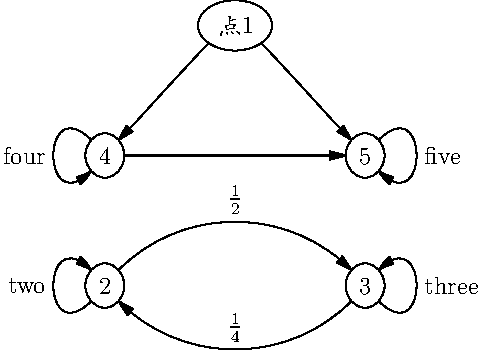
\includegraphics[angle=45,width=9cm]{test1.pdf}
\caption{`测试图片`} \label{test1}
\end{figure}
\end{lstlisting}

\begin{figure}[htbp]%位置选项
\centering
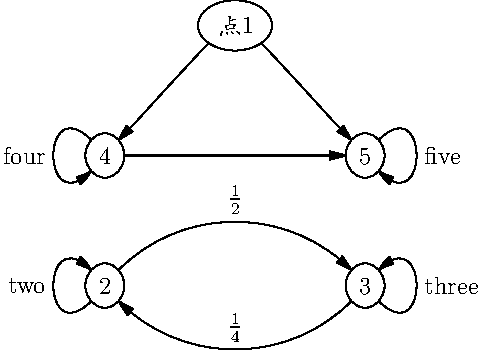
\includegraphics[angle=45,width=9cm]{test1.pdf}
\caption{测试图片} \label{test1}
\end{figure}


%%%%%%%%%%%%%%%%%%%%%%%%%%%%%%%%%%%%%%%%%%%%%%%%%%%%%%%%%%%%

\subsection{并排摆放,一个标题}
两幅图片中间不用换行符就会并排摆放了。
\begin{lstlisting}[language={[LaTeX]TeX}]
\begin{figure}[htbp]
\centering
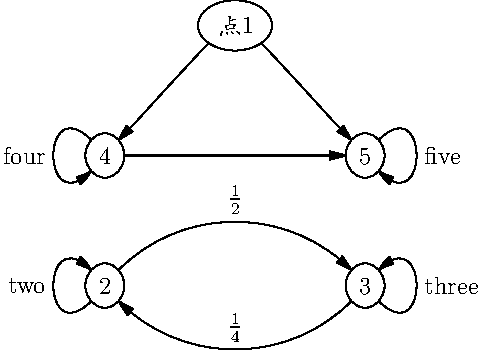
\includegraphics[width=5cm]{test1}
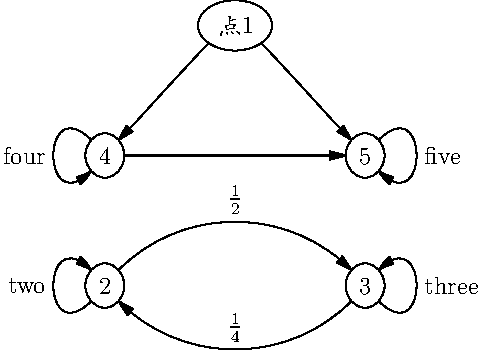
\includegraphics[width=5cm]{test1}
\caption{`并排一个标题`}
\end{figure}
\end{lstlisting}


\begin{figure}[htbp]
\centering
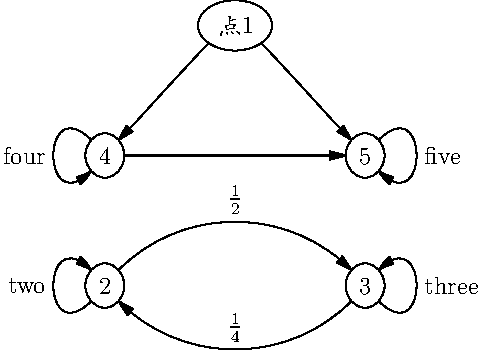
\includegraphics[width=5cm]{test1}
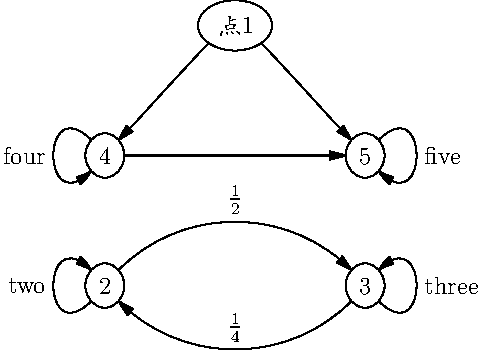
\includegraphics[width=5cm]{test1}
\caption{`并排一个标题`}
\end{figure}


%%%%%%%%%%%%%%%%%%%%%%%%%%%%%%%%%%%%%%%%%%%%%%%%%%%%%%%%%%%%

\subsection{并排摆放,各有标题}
主要是 minipage 环境的使用。
\begin{lstlisting}[language={[LaTeX]TeX}]
\begin{figure}[htbp]
\centering
\begin{minipage}[t]{0.3\textwidth}
\centering
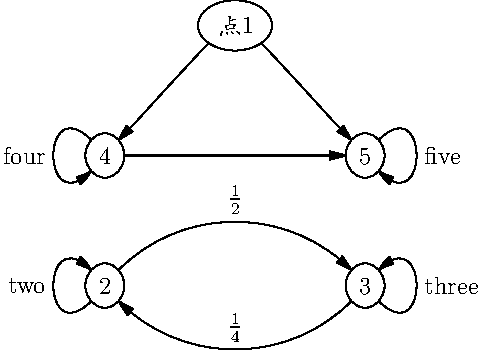
\includegraphics[width=5cm]{test1}
\caption{`左1`}
\end{minipage}
\begin{minipage}[t]{0.3\textwidth}
\centering
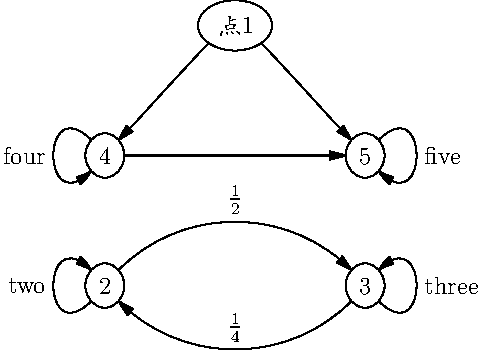
\includegraphics[width=5cm]{test1}
\caption{`左2`}
\end{minipage}
\end{figure}
\end{lstlisting}

\begin{figure}[htbp]
\centering
\begin{minipage}[t]{0.3\textwidth}
\centering
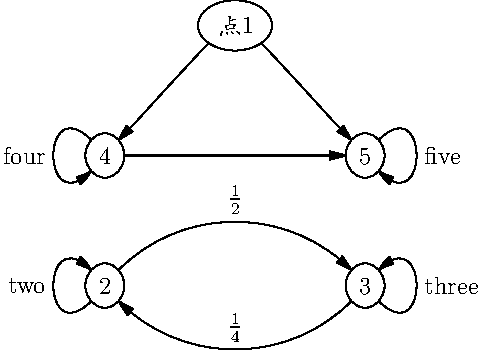
\includegraphics[width=5cm]{test1}
\caption{`左1`}
\end{minipage}
\begin{minipage}[t]{0.3\textwidth}
\centering
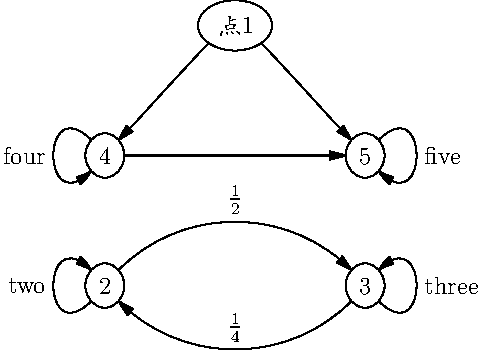
\includegraphics[width=5cm]{test1}
\caption{左2}
\end{minipage}
\end{figure}

\clearpage


%%%%%%%%%%%%%%%%%%%%%%%%%%%%%%%%%%%%%%%%%%%%%%%%%%%%%%%%%%%%

\subsection{图文绕排 picinpar宏包}
此宏包可将图形,表格,文字嵌入到文本中进行排版,提供三种环境 window,figwindow,tabwindow。

\index{命令!\verb$\begin{window}$}
\index{宏包!picinpar}

\begin{lstlisting}[language={[LaTeX]TeX}]

\begin{window}[`行数,列数,对象,`{`标题`}]
  `绕排文本`
\end{window}
\end{lstlisting}
\begin{description}
  \item[行数] 绕排对象上方的文字行数
  \item[列数] l,r,c对象在左,中,右的位置
  \item[对象] 可以为图形,表格,文本
  \item[标题] 对象的标题,如果是 figwindow 或 tabwindow 环境会加上图号和表号
\end{description}


\begin{figwindow}[2,r,{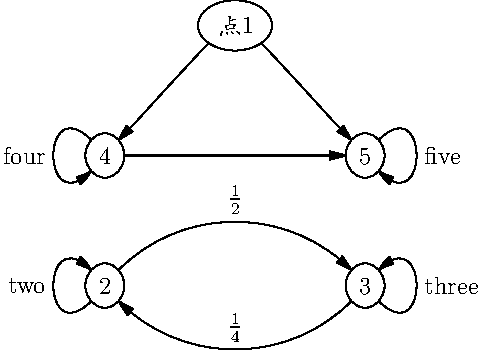
\includegraphics[width=8cm]{test1.pdf}},{绕排}]
平林漠漠烟如织,寒山一带伤心碧。暝色入高楼,有人楼上愁。
玉梯空伫立,宿鸟归飞急。何处是归程,长亭更短亭。泰戈尔
夏天的飞鸟,飞到我的窗前唱歌,又飞去了。秋天的黄叶,它
们没有什么可唱,只叹息一声,飞落在那里。时间可以摧毁世界上的一切,
可以把最坚固的城堡化作历史的残迹,可以把人类的偶像和权威化成灰烬,
可以把英雄的利剑化作孩子的玩物,可以把布满大森林的山脉变成布满珊瑚丛的无边的海洋。
然而,时间也可以造就一切,可以给猿人居住的洞穴变成金碧辉煌的高楼,可以给曾是残破的荒村变成繁华的城市,
也可以使无知的孩子变成百科全书式的学者,在自己的心中展开一个智慧的大星空。
\end{figwindow}


%%%%%%%%%%%%%%%%%%%%%%%%%%%%%%%%%%%%%%%%%%%%%%%%%%%%%%%%%%%%

\subsection{定制图形环境标题与间距 setlength}


%%%%%%%%%%%%%%%%%%%%%%%%%%%%%%%%%%%%%%%%%%%%%%%%%%%%%%%%%%%%


%\section{合并PDF}
\section{加入PDF,pdfpages宏包}
\index{命令!\verb$\includepdf$}
\index{命令!\verb$\includepdfmerge$}
\index{宏包!pdfpages}

\begin{shaded}
\begin{Verbatim}
\usepackage{pdfpages}
// 简略写法
\includepdfmerge{appendix/pcb.pdf,2-3}

// 插入多个PDF,同页显示
\includepdf
[pages={1,{},2-3},fitpaper=true,nup=2x2,landscape=true,
scale=0.8,delta=0mm 0mm, frame] {appendix/wangfan.pdf}


//连续的多个PDF
\includepdf[pages={1-3},fitpaper=false,nup=2x2,
landscape=false,delta=2mm 2mm,scale=0.8,
frame] {appendix/pcb.pdf}
\end{Verbatim}
\end{shaded}

\noindent
landscape 默认为 false,\\
frame 默认为 false,\\
fitpaper默认为false\\
scale默认为 1\\
nup 为 $n$ x $m$ ,n 为横向数目,m 为纵向数目。\\
加入目录和超链接\\
%addtotoc={(pagenumber),(section),(level),(heading),(label)}\\
加入图表目录\\
%addtolist={(pagenumber),(type),(heading),(label)}
lever : 1 为 section 2 为 subsection
pagenumber: 为 PDF 中要引用的页数\\
type= figure 或 table\\
heading 为目录中显示的标题\\
label 为引用标识\\


%%%%%%%%%%%%%%%%%%%%%%%%%%%%%%%%%%%%%%%%%%%%%%%%%%%%%%%%%%%%%%%%%%%%
%\section{环境}
\section{环境}
\subsection{自定义环境}

*号必须改为不同的名称以便设定不同的计数器。
\begin{Verbatim}[formatcom=\color{grass},frame=single]
\newcounter{buzhou_*} %不同环境计数器的名称也必需不同
\begin{list}
{\bfseries\sffamily 步骤\,\arabic{buzhou_*}:\hfill}
{\setlength{\parsep}{\parskip}
 \setlength{\itemsep}{0ex plus0.1ex}
 \setlength{\labelwidth}{4em}
 \setlength{\labelsep}{0.2em}
 \setlength{\leftmargin}{6.2em}
 \setlength{\rightmargin}{2em}
 \usecounter{buzhou_*} \setcounter{buzhou_*}{0}
 \upshape
}

\item 规则检查设置
\item 钻孔文件设置
\item ART
\item GERBE文件查看

\end{list}
\end{Verbatim}

\index{命令!\verb$\newcounter$}

结果如下所示\\
\newcounter{buzhou_test1}
\begin{list}
{\bfseries\sffamily 步骤\,\arabic{buzhou_test1}:\hfill}
{\setlength{\parsep}{\parskip}
 \setlength{\itemsep}{0ex plus0.1ex}
 \setlength{\labelwidth}{4em}
 \setlength{\labelsep}{0.2em}
 \setlength{\leftmargin}{6.2em}
 \setlength{\rightmargin}{2em}
 \usecounter{buzhou_test1} \setcounter{buzhou_test1}{0}
 \upshape
}



\item 规则检查设置
\item 钻孔文件设置
\item ART
\item GERBE文件查看

\end{list}

\subsection{默认环境}
有前面为阿拉拍数字和圆点的环境。

\index{环境!enumerate}
\index{环境!itemize}
\index{环境!description}

\begin{lstlisting}[language={[LATEX]TEX}]
`下面是阿拉伯数字列表`
\begin{enumerate}
  \item 
  \item 
  \item 
\end{enumerate}
`下面是圆点列表`
\begin{itemize}
  \item 
  \item 
  \item 
\end{itemize}
\begin{description}
  \item[`主题1名称`] 
  \item[`主题2名称`] 
  \item[`主题3名称`] 
\end{description}

\end{lstlisting}



\subsection{改变环境标号}


\index{命令!\verb$\labelitemi$}
\index{命令!\verb$\labelenumi$}
\index{环境!enumi}
\index{命令!\verb$\labelitemii$}
\index{命令!\verb$\labelenumii$}
\index{环境!enumii}
\index{命令!\verb$\labelitemiii$}
\index{命令!\verb$\labelenumiii$}
\index{环境!enumiii}
\index{命令!\verb$\labelitemiv$}
\index{命令!\verb$\labelenumiv$}
\index{环境!enumiv}



\subsubsection{使用 \LaTeX 命令}

itemize 的分层标号如下

\begin{itemize}
  \item
  \begin{itemize}
           \item
           \begin{itemize}
             \item
             \begin{itemize}
               \item
             \end{itemize}
           \end{itemize}
         \end{itemize}
\end{itemize}

enumerate 的各层标号如下

\begin{enumerate}
  \item
  \begin{enumerate}
    \item
    \begin{enumerate}
      \item
      \begin{enumerate}
        \item
      \end{enumerate}
    \end{enumerate}
  \end{enumerate}
\end{enumerate}

itemize 和 enumerate 的标签命令保存在以下命令中:

\begin{shaded}
  \begin{Verbatim}
    \labelitemi  \labelitemii \labelitemiii \labelitemiv
    \labelenumi  \labelenumii \labelenumiii \labelenumiiv
  \end{Verbatim}
\end{shaded}

其计数器没有倒斜线,为

\begin{framed}
  \begin{Verbatim}
    enumi  enumii enumiii enumiv
  \end{Verbatim}
\end{framed}

将 enumerate 的首标号改为 a),次层标号改为 1)代码如下:

\begin{shaded}
  \begin{Verbatim}
\renewcommand{\labelenumi}{\alph{enumi})}
\renewcommand{\labelenumii}{\arabic{enumii})}
  \end{Verbatim}
\end{shaded}


同理,将 itemize 的第二层标号 - 改为 + 代码如下:


\begin{shaded}
  \begin{Verbatim}
\renewcommand{\labelitemii}{+}
  \end{Verbatim}
\end{shaded}

以上命令放在导言区对所有命令起作用,放在当前环境则只对当前环境起作用。


\subsubsection{使用 enumerate 宏包}


enumerate 环境更换标号的快捷方式

\begin{cmd}[label=enuemerate 更换标号]
  \begin{enumerate}[A a I i 或 1 + 任意字符]
  \item
  \end{enumerate}
  注意:如果字符中包含了 A a I i 或 1 中一个,需用{}框起来
\end{cmd}

\begin{lstlisting}[language={[LaTeX]TeX}]
\begin{enumerate}[`例` i.]
\item one one one one one one one
one one one one\label{LA}
\item two
\begin{enumerate}[{example} a)]
\item one of two one of two
one of two\label{LB}
\item two of two
\end{enumerate}
\item two of two
\end{enumerate}
\end{enumerate}
\begin{enumerate}[{A}-1]
\item one\label{LC}
\item two
\end{enumerate}
\ref{LA}, \ref{LB},\ref{LC}
\end{lstlisting}

显示效果如下:

\begin{enumerate}[例 i.]
\item one one one one one one one
one one one one \label{LA}
\item two

\begin{enumerate}[{example} a)]
\item one of two one of two
one of two \label{LB}
\item two of two
\end{enumerate}

\item two of two
\end{enumerate}

\begin{enumerate}[{A}-1]
\item one \label{LC}
\item two
\end{enumerate}

引用效果如下:\ref{LA},\ref{LB},\ref{LC}

%\subsection{短列表环境 shortlst}
%
%\index{命令!\verb$\begin{shortitemize}$}
%\index{命令!\verb$\begin{shortenumerate}$}
%\index{宏包!shortlst}
%
%如下所示,将许多可以简短条目在一行内显示出来有 shortitemize 和 shortenumerate 两种形式。
%\begin{shaded}
%  \begin{Verbatim}
%  \usepackage{shortlst}
%    \begin{shortitemize}
%      \item ...
%    \end{shortitemize}
%
%    \begin{shortenumerate}
%      \item \laber{...}...
%    \end{shortenumerate}
%    我选择\ref{...}
%  \end{Verbatim}
%\end{shaded}
%
%\begin{shortenumerate}
%  \item 短列表1  \item 短列表2  \item 短列表3  \item 短列表4  \item 短列表短列表短列表5 \item 短列表6  \item 短列表7
%    \item 短列表8  \item 短列表9  \item 短列表短列表短列表短列表10  \item 短列表11  \item \label{short12}短列表12\
%\end{shortenumerate}
%我选择\ref{short12}。
%\begin{shortitemize}
%  \item 短列表1  \item 短列表2  \item 短列表3  \item 短列表4  \item 短列表短列表短列表5 \item 短列表6  \item 短列表7
%    \item 短列表8  \item 短列表9  \item 短列表短列表短列表短列表10  \item 短列表11  \item 短列表12
%\end{shortitemize}




%%%%%%%%%%%%%%%%%%%%%%%%%%%%%%%%%%%%%%%%%%%%%%%%%%%%%%%%%%%%%%%%%%%%

%\section{参考文献}
\section{参考文献}
\index{命令!\verb$\bibiographystyle{}$}
\index{命令!\verb$\bibitem$}
\index{命令!\verb$\bibliography{}$}
常见的引用格式 bibliographystyle\{格式\} 有下面4种\\


\begin{tabular}{ll}
  % after \\: \hline or \cline{col1-col2} \cline{col3-col4} ...
  plain & 文献按字母顺序列出 author year  title 这三种字母顺序比较 \\
  unsrt & 引用顺序列出\\
  abbrv & 同 plain 但 firstname,month,title,journal 变成缩写\\
  alpha & 引用处用作者年份代替数字 \\

\end{tabular}

\begin{lstlisting}[language={[LaTeX]TeX}]
\bibliographystyle{plain}
\bibliography{reference/REF}

\begin{thebibliography}{99} %`99为最多引用文献数目`
\setlength{\parskip}{0pt}  %`段落之间的竖直距离`

\bibitem[`指定标号`]{`引用标签`} 251289-001  Intel Low Pin Count~~[S]
\bibitem[]{} PCI Local Bus Specification Revision 3.0~~[S]

\end{thebibliography}
\thispagestyle{fancy} \fancyhead[R]{\song\wuhao `参考文献`}
\addcontentsline{toc}{chapter}{`参考文献`}        %`加入参考文献到目录`
\end{lstlisting}


%%%%%%%%%%%%%%%%%%%%%%%%%%%%%%%%%%%%%%%%%%%%%%%%%%%%%%%%%%%%%%%%%%%%

%\section{超链接 href}
\section{超链接}
\subsection{选项配置}
\textcolor[rgb]{0.50,0.00,0.50}{ 颜色的应用:} \newline 1.
红色(Red)用来作为内部的链接 \newline 2.
红紫色(Magenta)用来作为web或者email地址的链接。 \newline 3.
蓝色(有时候是绿色,还有少数是红色)用来标示强调的词或者说明性的词。
\newline
\textcolor[rgb]{0.50,0.00,0.50}{书签(Bookmarks) }\newline 1.
Options:选择hyperref的四个位置: \newline (a) 全局: $\backslash
$documentclass[. . . ] \newline (b) 用宏包: $\backslash
$usepackage[. . . ] \newline (c) 配置文件: 用$\backslash
$hypersetup配置hyperref.cfg \newline (d) 在宏包之后: $\backslash
$hypersetup{\{}. . . {\}} \newline 2. 影响书签的选项 \newline (a)
bookmarks:使得书签有效(缺省为true).如果宏包已经装载,那么这个选项不能应用。
\newline
(b) bookmarksnumbered: 把节的标号放入标签(缺省:false)。 \newline (c)
bookmarksopen: 打开书、签树(缺省: false). \newline (d)
bookmarksopenlevel:书签打开的层数(缺省: maxdimen). \newline

\textcolor[rgb]{0.50,0.00,0.50}{ hyperref的设置} \newline
1.应用如下设置超链接的颜色是相同的 \newline $\backslash
$documentclass[11pt]{\{}article{\}} \newline $\backslash
$usepackage{\{}color{\}} \newline $\backslash $ifx$\backslash
$pdfoutput$\backslash $undefined \newline $\backslash
$usepackage[dvips]{\{}graphicx{\}} \newline $\backslash
$usepackage[dvipdf, \newline pdfstartview=FitH, CJKbookmarks=true,
bookmarksnumbered=true, \newline bookmarksopen=true,
colorlinks=false, colorlinks=black, \newline pdfborder=100,
citecolor=black ]{\{}hyperref{\}} \newline $\backslash
$AtBeginDvi{\{}$\backslash $special{\{}pdf:tounicode
GBK-EUC-UCS2{\}}{\}} {\%} GBK -> Unicode \newline $\backslash $else
\newline $\backslash $usepackage[dvipdf, \newline pdfstartview=FitH,
CJKbookmarks=true, bookmarksnumbered=true, \newline
bookmarksopen=true, colorlinks=true, citecolor=black
]{\{}hyperref{\}}
\newline
$\backslash $usepackage[pdftex]{\{}graphicx{\}} \newline $\backslash
$fi \newline 2.应用如下设置超链接的颜色不同的 \newline $\backslash
$ifx$\backslash $pdfoutput$\backslash $undefined \newline
$\backslash $usepackage[CJKbookmarks=true,dvipdfm, \newline
pdfstartview=FitH,{\%}开始时候页面的大小,是正常的页面,即100{\%},注释掉的话页面大小为50{\%}
\newline
]{\{}hyperref{\}} $\backslash $else \newline $\backslash
$usepackage[CJKbookmarks=true,pdftex, \newline
pdfstartview=FitH,{\%}开始时候页面的大小,是正常的页面,即100{\%},注释掉的话页面大小为50{\%}
]{\{}hyperref{\}}

$\backslash $fi \newline
这里仅仅说明了hyperref的设置,可以照旧应用其他宏包(如CJK)。但是注意hyperref应该放在所有宏包的最后。
\newline

hyperref 的选项设置如\ref{hyperref_config}所示。

\begin{center}
\rowcolors{1}{lightgray}{}
\begin{longtable}[H]{p{3.2cm}p{3cm}p{3cm}p{3cm}}
\caption{hyperref 参数选项设置} \label{hyperref_config} \\
\toprule \multicolumn{1}{c}{\textbf{选项}} &
\multicolumn{1}{c}{\textbf{作用 }} &
\multicolumn{1}{l}{\textbf{参数 }}  &
\multicolumn{1}{c}{\textbf{说明 }}\\ \midrule
\endfirsthead

\multicolumn{4}{c}%
{{\centering \kai\thetable{}hyperref 参数选项设置-~- 接上页}} \\
\toprule \multicolumn{1}{c}{\textbf{选项}} &
\multicolumn{1}{c}{\textbf{作用 }} &
\multicolumn{1}{l}{\textbf{参数 }}  &
\multicolumn{1}{c}{\textbf{说明 }}\\ \midrule
\endhead
\multicolumn{3}{r}{{\kai 接下页}} \\ \bottomrule
\endfoot
\bottomrule
\endlastfoot

a4paper & 使用A4纸张 && \\
a5paper & 使用A5纸张 && \\
anchorcolor &链接锚文本颜色 & black &默认值\\
b5paper &使用B5纸张&& \\
backref &反向引用&false &默认值\\
baseurl &基本URL &empty &默认值\\
bookmarks &生成书签&true &默认值\\
bookmarksnumbered &书签中章节编号&true &默认值\\
bookmarksopen &书签目录展开&true &默认值\\
bookmarksopenlevel &书签目录层次&
\verb|\maxdimen| &默认值,最高1或2或3... 可选值\\

%%%%%%%%%%%%%%%%%%%%%%%%%%%
bookmarkstype
&
书签目录类型
&
toc\par
lof\par
lot
&
章节目录,默认\par
图形目录 \par
表格目录
\\
%%%%%%%%%%%%%%%%%%%%%%%%%%%
breaklinks  &允许链接断行 &false& 默认值\\
citebordercolor &引用标记边框颜色&{0 1 0}& 默认值\\
citecolor &引用标记颜色&green& 默认值\\
colorlinks &彩色链接&true &默认值\\
CJKbookmarks &中文书签&true &默认值\\
debug & log诊断信息打印&false& 默认值\\
draft & 超文本选项失效&false& 默认值\\
dvipdf &使用dvipdf驱动&&\\
dvipdfm &使用dvipdf驱动&&\\
dvips &使用dvips驱动&&\\
dvipsone &使用dvipsone驱动&&\\
dviwindo &使用dviwindo驱动&&\\
encap &设置超索引符号&&\\
executivepaper &7.25in×10.5in纸&&\\
extension &设置文件扩展名
&
dvi\par
ps、pdf
&
默认值\par
... 可选值
\\
filebordercolor &文件链接边框颜色&{0 .5 .5}& 默认值\\
filecolor &文件链接颜色&cyan &默认值\\
final& 超文本选项生效&true &默认值\\
frenchlinks &链接字体为小型大写&false& 默认值\\
hyperfigures &图形链接&false &默认值\\
hyperindex &索引链接&true &默认\\
hypertex &hypertex驱动&&\\
hypertexnames &用推测名称链接&true &默认值\\
implicit &内部定义&true &默认值\\

latex2html &latex2html驱动&&\\
legalpaper &8.5in×14in纸张&&\\
letterpaper &8.5in×11in纸张&&\\
linkbordercolor &内部链边框接颜色&{1 0 0} &默认值\\
linkcolor &内部链接颜色&red &默认值\\
linktocpage &目录页码链接&false& 默认值\\
menubordercolor &菜单链接框颜色&{1 0 0} &默认值\\
menucolor& 菜单链接颜色&red &默认值\\
naturalnames &使用编译名&false &默认值\\
nesting & 允许链接嵌套&false& 默认值\\
pageanchor &每页增设页锚&true& 默认值\\
pagebackref &反向引用页码&false &默认值\\
pagebordercolor &页链接框颜色&{1 1 0} &默认值\\
pagecolor &页链接颜色&red &默认值\\

pdfauthor &作者&&\\

%%%%%%%%%%%%%%%%%%%%%%%%%%%%%
pdfborder
&
链接边框
&
{0 0 0} \par
{0 0 1}
&
默认值,无框 \par
可选值,有框
\\
%%%%%%%%%%%%%%%%%%%%%%%%%%%%%%%%%%
pdfborderstyle
&
连接边框样式
&
{/S/U} \par
{/S/D/D[3 2]/W 1}
&
下划线\par
虚线框\\

pdfcenterwindow &在屏幕上居中窗口&true& 默认值\\
pdfcreator& 应用程序(需用命令\verb|\hypersetup|设置)&
LaTeX with hy-perref
package &默认值\\

pdfdirection &
方向设定
&
L2R\par
R2L
&
由左至右\par
由右至左\\
pdfdisplaydoctitle &显示文件标题&true &默认值\\

%%%%%%%%%%%%%%%%%%%%%%%%%%%%%%%%%%%%%%%%%%%%
pdfduplex &双面打印
&
Simplex \par
DuplexFlipShort-Edge \par
DuplexFlipLong-Edge
&
单面 \par
双面短边装订 \par
双面长边装订\\

%%%%%%%%%%%%%%%%%%%%%%%%%%%%%%%%%%%%
pdfescapeform &容错&false &默认值\\


pdffitwindow &调整窗口&false &默认值\\
pdfhighlight &点击链接时显示
&
/I \par
/N \par
/O \par
/P
&
翻转,默认值 \par
外观不变 \par
出现黑色边框 \par
出现黑色半框\\
%%%%%%%%%%%%%%%%%%%%%%%%%%%%%%%%%%%%

pdfkeywords &关键字&&\\
pdflang &PDF标识符&&\\
pdfmenubar &显示菜单栏&true &默认值\\
pdfnewwindow &生成新窗口&false &默认值\\
pdfnumcopies &打印份数 1 或 2 或 3...&&\\

%%%%%%%%%%%%%%%%%%%%%%%%%%%%%%%%%%%%%%%%%
pdfnonfullscreen-\par
pagemode
&
全屏显示样式
&
UseNone \par
UseOutlines \par
UseThumbs \par
FullScreen
&
无书签缩略图 \par
附书签 \par
附缩略图 \par
无书签缩略图
\\
%%%%%%%%%%%%%%%%%%%%%%%%%%%%%%%%%%%%%%%%%
pdfpagelayout
&
页面布局
&
TwoColumnLeft \par
SinglePage \par
OneColumn \par
TwoColumnRight
&
对开,默认值 \par
单页 \par
连续 \par
连续-对开
\\
%%%%%%%%%%%%%%%%%%%%%%%%%%%%%%%%%%%%%%%%%
pdfpagemode &
文件打开模式
&
UseNone 默认\par
UseThumbs\par
UseOutlines\par
FullScreen
&
无书签和缩略图\par
显示缩略图\par
显示书签\par
全屏显示
\\
pdfpagelabels &
底部页码样式:\par
“v(第 5/15 页)”\par
或“第 5/15 页”
&true& 默认值\\

pdfpagescrop & 设置裁切尺寸&例如:\{53 486 389 754\}&\\

pdfpagetransition &
页面过渡样式\par
参数后可加子参数:\par
/Dm、/Bi、/M、/H
/V、/I、/O\par
(需全屏显示模式)
&
Dissolve \par
Wipe \par
Split \par
Glitter \par
Blinds \par
Box
&
马赛克散开 \par
下拉帘幕 \par
上下拉帘幕 \par
溶化 \par
百叶窗翻转 \par
渐缩框
\\

pdfpicktraybypdfsize  & 纸张自动选择&true& 默认值\\
pdfprintarea & 打印范围&参数与pdfviewarea相同&\\
pdfprintclip & &参数与pdfviewarea相同&\\
pdfprintpagerange & 设置打印页码范围{n n}&&\\

pdfprintscaling &
打印放大率
&
AppDefault  \par
None
&
默认\par
无
\\

pdfproducer &PDF加工程序需用\verb|\hypersetup| 命令设置&&\\
pdfstartpage &打开到页码& 1 &默认值\\

%%%%%%%%%%%%%%%%%%%%%%%%%%%%%%%%%%%%%%%%%
pdfstartview &
PDF文件初始视图&
/Fit \par
FitH \par
FitV \par
FitR \par
FitB \par
FitBH \par
FitBV \par
XYZ \par
&
默认值 \par
页宽适合窗口 \par
页高适合窗口 \par
适合窗口对角线\par
版面适合窗口\par
版宽适合窗口\par
版高适合窗口\par
自定放大率\par
\\
%%%%%%%%%%%%%%%%%%%%%%%%%%%%%%%%%%%%%%%%%
pdfsubject &文件主题 &&\\
pdftex &pdflatex驱动 &&\\
pdftitle &文件标题 &&\\
pdftoolbar &显示工具栏&true& 默认值\\
pdfview &链接默认视图&参数与pdfstartview相同&\\

%%%%%%%%%%%%%%%%%%%%%%%%%%%%%%%%%%%%%%%%%
pdfviewarea &显示区域 &&\\
MediaBox & 媒体框 &&\\
CropBox &裁切框 &&\\
BleedBox &出血框 &&\\
TrimBox &修剪框 &&\\
ArtBox &作品框 &&\\

%%%%%%%%%%%%%%%%%%%%%%%%%%%%%%%%%%
pdfviewclip &剪贴区域&参数与pdfviewarea相同&\\
pdfwindowui &显示窗口控件 &true& 默认值\\
plainpages &页锚编号&true &默认值\\

ps2pdf &ps2pdf驱动&&\\
raiselinks &抬高链接&false &默认值\\
runbordercolor &run链接边框颜色&\{0 .7 .7\} &默认值\\
setpagesize &用命令设置页面尺寸&true &默认值\\

tex4ht& TeX4ht驱动&&\\
textures &Textures 驱动&&\\
unicode &Unicode 编码书签&false& 默认值\\
urlbordercolor &URL 链接边框颜色&\{0 1 1\} &默认值\\
urlcolor &网页与电邮链接颜色&magenta &默认值\\
verbose &附加信息&false &默认值\\
vtex &使用VTeX驱动&&\\
vtexpdfmark &vtexpdfmark驱动&&\\
xetex &使用XeTeX驱动&&\\
\end{longtable}
\end{center}
\subsection{文本超链接}

设置文本超链接,从文本的一处链接到另一处。 \newline 例如: \newline
$\backslash $hypertarget{\{}bilevel{\}}{\{}bilevel programming
problem{\}}设置锚点 \newline $\backslash
$hyperlink{\{}bilevel{\}}{\{}BLP{\}} 设置链接 \newline
\newline
\textcolor[rgb]{0.50,0.00,0.50}{效果为:} \newline bilevel
programming problem \newline BLP \newline 则点BLP可以链接到bilevel
programming problem \newline

\subsection{EMAIL 超链接}

链接到email \newline 例如: \newline $\backslash
$href{\{}mailto:username@whu.edu.cn{\}}{\{}username@whu.edu.cn{\}}
\newline \textcolor[rgb]{0.50,0.00,0.50}{效果为:} \newline
username@whu.edu.cn \newline
username@whu.edu.cn为显示的内容可以修改为你需要的内容。 \newline

\subsection{网址超链接}
网址的超链接(url,href等的应用) \newline 例如: \newline $\backslash
$url{\{}http://www.whu.edu.cn/{\}}链接到http://www.whu.edu.cn/
\newline
效果为: \newline http://www.whu.edu.cn/ \newline $\backslash
$nolinkurl{\{}http://www.whu.edu.cn/{\}}是无链接输入网址的形式。
\newline
$\backslash
$href{\{}http://www.whu.edu.cn/{\}}{\{}武汉大学{\}}链接到http://www.whu.edu.cn/
\newline
\textcolor[rgb]{0.50,0.00,0.50}{效果为:} \newline 武汉大学 \newline
用$\backslash $href也可以链接硬盘上的文件,例如: \newline
$\backslash $href{\{}C:/paper/example1.pdf{\}}{\{}example1.pdf{\}}
\newline 效果为: \newline example1.pdf \newline
在Dvi文件下可以正常打开文件example1.pdf,但是需要在acrobat中设置才能正常用acrobat来打开文件example1.pdf。而且该命令还支持相对路径,但是路径中不能用中文。
\newline
\subsection{直接打开链接文件}
只要超级链接的地址前加上run:就可以了。例如,用hyperref宏包的href命令创建一个链接打开一个文件some.file就可以用$\backslash$href\{run:path/to/some.file\}\{some
link\}。
这样的话,我们就可以直接在PDF中点击链接打开文件,而不必先切换界面再去点文件了。其实run跟http、ftp等一样,都是协议。

\subsection{图表超链接}
例如: \newline $\backslash $begin{\{}figure{\}} \newline
{\{}$\backslash
$includegraphics[width=2.53in,height=1.75in]{\{}figurename.eps{\}}{\}}
\newline
$\backslash $caption{\{}caption of figure{\}} $\backslash
$label{\{}label of figure{\}} \newline $\backslash
$end{\{}figure{\}} \newline $\backslash $begin{\{}table{\}} \newline
..... $\backslash $caption{\{}caption of table{\}} $\backslash
$label{\{}label of table{\}} \newline $\backslash $end{\{}table{\}}
\newline 然后用ref{\{}label of figure(table){\}}
就可以得到图或表引用的超链接,但这仅仅将编号的数字变成超链接,即图1,表2,如将相应的文字也超链接,即:图1,表2,则可以利用hyperref
包中的$\backslash $autoref功能。只要将引用图的$\backslash
$ref{\{}label{\}}换成$\backslash
$autoref{\{}label{\}}即可。但有个问题就是,这样处理的结果是英文的,即``Figure
1'',或是"Table
2"。要想超链接的文字变成``图1''或者"表2",可以预先做如下的重定义:
\newline $\backslash $renewcommand$\backslash
$figureautorefname{\{}图{\}}. $\backslash $renewcommand$\backslash
$tableautorefname{\{}表{\}}. \newline
对于公式、章节等要达到同等的效果可以类似考虑,不再一一说明。
\newline 注意:如果在图或者表格环境中没有caption或者它与$\backslash
$label分开那么引用时没有图表编 \newline 号。即当用$\backslash
$autoref{\{}label{\}}时仅有Table(Figure)。 \newline

\subsection{公式超链接}
例如: \newline $\backslash $begin{\{}equation{\}}$\backslash
$label{\{}equation{\}}
\newline
x+y=z \newline $\backslash $end{\{}equation{\}} \newline
用ref{\{}label of equation{\}}
可以将公式的引用作为超链接。对于能够产生公式编号的数学环境命令类似考虑,不再一一举例说明。
\newline

\subsection{文献目录超链接}
只要用了宏包hyperref就可以产生他们的超链接。对于文献的引用方法没有改变,但是hyperref宏包不能与cite宏包同时应用,
而且也不能使得文献压缩引用。 \newline

\subsection{定理引理推论中文环境超链接}
例如: \newline 在前面定义$\backslash
$newtheorem{\{}Theorem{\}}{\{}Theorem{\}}[section],由代码 \newline
$\backslash $begin{\{}Theorem{\}}$\backslash $label{\{}theorem1{\}}
\newline 这是一个定理的例子 \newline $\backslash $end{\{}Theorem{\}}
\newline 4 \newline 然后用$\backslash
$ref{\{}theorem1{\}}就可以得到该定理的超链接。其它的类似考虑。对于enumerate,itemize等环境也可以得到引用的超链接。
\newline
\subsection{章节的引用}
例如: \newline $\backslash $section{\{}section's
name{\}}$\backslash $label{\{}label of section's name{\}} \newline
用ref{\{}label of section's name{\}}
可以将节的引用作为超链接,对于部分、章以及子节等类似考虑。 \newline
\subsection{注释超链接}
把$\backslash $ref替换为$\backslash $ref*可以注释掉超链接的形式。
\newline

\subsection{PDF 属性设置}
以下命令放在文档中。
\begin{lstlisting}
  \hypersetup{
  pdfkeywords={latex,pgf,asy,beamer}, %`关键词`
  pdfsubject={latex}, %`主题`
  pdfauthor={`王凡`}, %`作者`
  pdftitle={xelatex `笔记`}, %`标题`
  pdfcreator={texlive2011}}
\end{lstlisting}



%%%%%%%%%%%%%%%%%%%%%%%%%%%%%%%%%%%%%%%%%%%%%%%%%%%%%%%%%%%%%%%%%%%%

%\section{下划线 ulem}
\section{下划线}
\subsection{ulem 宏包}
\index{命令!\verb$\uline$}
\index{命令!\verb$\uuline$}
\index{命令!\verb$\uwave$}
\index{命令!\verb$\sout$}
\index{命令!\verb$\xout$}
\index{宏包!ulem}

使用方式,因为 ulem 宏包重新定义了加粗 $\backslash$emph
命令,为避免加粗定义被取消,用[normalem]选项来加入宏包。
\begin{lstlisting}[language={[LaTeX]TeX}]
 \usepackage[normalem]{ulem}%`加入宏包`
 \uline{text} %`下划单线`
 \uuline{text}%`双横线`
 \uwave{text}%`波浪线`
 \sout{text}%`中间删除线`
 \xout{text}%`斜线阴影状`
\end{lstlisting}

\fbox{ \uline{text}  \uuline{text} \uwave{text} \sout{text}
\xout{text}}

%\subsection{CJKfntef 宏包}
%\index{命令!\verb$\CJKunderline$}
%\index{命令!\verb$\CJKunderdot$}
%\index{命令!\verb$\CJKunderwave$}
%\index{命令!\verb$\CJKunderdbline$}
%\index{命令!\verb$\CJKsout$}
%\index{命令!\verb$\CJKxout$}
%\index{宏包!CJKntef}
%
%下划线可换行,可与 color
%宏包嵌套,CJKunderline的一个用途是利用全角空格产生可自动分行的空下划线,可用于填空题。:
%\begin{enumerate}
%    \item 分散对齐
%    \item 加点
%    \item 下划线
%\end{enumerate}
%
%\begin{lstlisting}[language={[LaTeX]TeX}]
% \usepackage{CJKfntef}%`加入宏包`
% \CJKunderline{`文 本`} %`下划单线`
% \CJKunderline*{`文 本`}
% \CJKunderdot{`文 本`} %`下划点`
% \CJKunderwave*{`文 本`}
% \CJKunderwave*{`文 本`}
% \CJKunderdblline{`文 本`}
% \CJKunderdblline*{`文 本`}
% \CJKsout{`文 本`}
% \CJKsout*{`文 本`}
% \CJKxout{`文 本`}
% \CJKxout*{`文 本`}
% \begin{CJKfilltwosides}{40mm}
%`两端分散对齐`\\
%`分散对齐`\\
%`汉字加点`\\
%\end{CJKfilltwosides}
%\end{lstlisting}
%
%\index{命令!\verb$\begin{CJKfilltwosides}$}
%
%效果如下:\\
% \CJKunderline{文 本}
% \CJKunderline*{文 本}
% \CJKunderdot{文 本}
% \CJKunderwave*{文 本}
% \CJKunderwave*{文 本}
% \CJKunderdblline{文 本}
% \CJKunderdblline*{文 本}
% \CJKsout{文 本}
% \CJKsout*{文 本}
% \CJKxout{文 本}
% \CJKxout*{文 本}\\
%\begin{CJKfilltwosides}{40mm}
%两端分散对齐\\
%分散对齐\\
%汉字加点\\
%\end{CJKfilltwosides}


\subsection{扩展符号线段 makebox}

\index{命令!\verb$\makebox$}
\index{命令!\verb$\dotfill$}
\index{命令!\verb$\hrulefill$}
\index{命令!\verb$\downbracefill$}
\index{命令!\verb$\upbracefill$}
\index{命令!\verb$\leftarrowfill$}
\index{命令!\verb$\rightarrowfill$}
\index{命令!\verb$\fbox$}
\index{命令!\verb$\shortstack$}
\index{命令!\verb$\noindent$}

\begin{shaded}
  \begin{Verbatim}
  \noindent
    \makebox[6cm]{\dotfill}\\
    \makebox[6cm]{\hrulefill}\\
    \makebox[6cm]{\downbracefill}\\
    \makebox[6cm]{\upbracefill}\\
    \makebox[6cm]{\leftarrowfill}\\
    \fbox{\shortstack{左边\\文本}}
    \rightarrowfill
    \fbox{\shortstack{右边\\文本}}
  \end{Verbatim}
\end{shaded}

效果如下:

  \noindent
    \makebox[6cm]{\dotfill}\\
    \makebox[6cm]{\hrulefill}\\
    \makebox[6cm]{\downbracefill}\\
    \makebox[6cm]{\upbracefill}\\
    \makebox[6cm]{\leftarrowfill}\\
    \fbox{\shortstack{左边\\文本}}
    \rightarrowfill
    \fbox{\shortstack{右边\\文本}}


\subsection{线段盒子}

\index{命令!\verb$\hrule$}
\index{命令!\verb$\framebox$}

主要参数有一条粗线的长度,宽度及与当前行基线的位置\\

\begin{shaded}
  \begin{Verbatim}
  \rule[垂直位移]{宽度}{高度}
    粗线\rule{6mm}{3mm}水平\\
    粗线\rule[1mm]{6mm}{3mm}水平\\
    \parbox{30mm}{Did you know \par \rule[4mm]{37mm}{1.6pt}}\\
    \framebox{\rule{9cm}{1pt}\rule{1pt}{5mm}}\\
    \framebox{\rule{9cm}{0pt}\rule{0pt}{5mm}}
  \end{Verbatim}
\end{shaded}

\noindent
    粗线\rule{6mm}{3mm}水平\\
    粗线\rule[1mm]{6mm}{3mm}水平\\
    \parbox{30mm}{Did you know?\par \rule[4mm]{37mm}{1.6pt}}\\
    \framebox{\rule{9cm}{1pt}\rule{1pt}{5mm}}\\
    \framebox{\rule{9cm}{0pt}\rule{0pt}{5mm}} %起支撑作用


%%%%%%%%%%%%%%%%%%%%%%%%%%%%%%%%%%%%%%%%%%%%%%%%%%%%%%%%%%%%%%%%%%%%

%\section{脚注}
\section{脚注边注设计}
\index{命令!\verb$\footnote$}

\subsection{脚注编号 footnote}
\subsubsection{使用方法}
\begin{lstlisting}[language={[LaTeX]TeX}]
\footnote[`序号`]{`脚注内容`}
\end{lstlisting}

\subsubsection{调整脚注序号}
不带序号的脚注前加以下命令:
\begin{lstlisting}[language={[LaTeX]TeX}]
\renewcommand{\thefootnote}{}%`清除脚注序号`
\end{lstlisting}
序号改为字母形式:
\begin{lstlisting}[language={[LaTeX]TeX}]
\renewcommand{\thefootnote}{\alph{footnote}}
\end{lstlisting}
脚注序号是以每章第一个脚注为 1 开始排序,要以全文为单位排序可用
remmreset 宏包,并在后加入以下命令:
\begin{lstlisting}[language={[LaTeX]TeX}]
\makeatother
\@removefromreset{footnote}{chapter}
\makeatother
\end{lstlisting}
\subsubsection{调整脚注字体}
默认为中文宋体,英文罗马体,尺寸为 footnotesize。
可用下述命令修改:
\begin{lstlisting}[language={[LaTeX]TeX}]
\renewcommand{\footnotesize}{\small\sf\fangsong}
\end{lstlisting}

\subsubsection{小页环境 minipage 中的脚注}
\index{命令!\verb$\footnotemark$}
脚注在小页的底部,而不是页面底部。小页环境中脚注序号为小写英文字母,计数器为 mpfootnote。

如果要求小页脚注与普通脚注统一,可用 \verb|\footnotemark| 和  \verb|\footnotetext{}| 来插入脚注,
 \verb|\footnotemark| 插在要标注的地方, \verb|\footnotetext{}|放在小页环境后。括号内为脚注内容。

\subsubsection{表格中的脚注}
tabular 和 array 不支持脚注命令\verb|\footnote| ,longtable 和 tabularx 表格环境中可使用,脚注在页底,
如要在表格下实现脚注,可将 longtable 或 tabularx 嵌入 minipage 中。

但实现的表格脚注长度可能超过表格宽度,因此可使用宏包 threeparttable 来实现表格环境的脚注,可实现三种表格环境
tabluar、tabluarx、tabluar$*$ 三种环境的表格脚注。
使用要点:threeparttable 环境是不浮动的,如果要浮动,可再置于 table 或 table$*$ 环境中。
\index{命令!\verb$\begin{threeparttable}$}
\index{宏包!threeparttable}
\begin{lstlisting}[language={[LaTeX]TeX}]
\usepackage[]{threeparttable}
%`可选参数有:`
%para `所有脚注作为一段,默认每个脚注一段`
%flushleft  `脚注左侧对齐,默认缩进 1.5em`
%online  `标记与标注同尺寸,默认为上标形式`

\tnote{`标记序号`}
%`在表格后用以下代码`
\begin{center}
\begin{threeparttable}
\caption{`表格标注`}
\begin{tabular}{ll}
\toprule
`我是表格`\tnote{a} & `是什么表格` \\
`表` & `测试数据,加长表格` \tnote{b}\\
\bottomrule
\end{tabular}
\begin{tablenotes} \footnotesize
  \item[a] `我是表格标注1`
  \item[b] `我是表格标注2`
\end{tablenotes}
\end{threeparttable}
\end{center}
\end{lstlisting}

\begin{center}
\begin{threeparttable}
\caption{表格标注}
\begin{tabular}{ll}
\toprule
我是表格\tnote{a}&是什么表格\\
表&测试数据,加长表格\tnote{b}\\
\bottomrule
\end{tabular}
\begin{tablenotes} \footnotesize
  \item[a] 我是表格标注1
  \item[b] 我是表格标注2
\end{tablenotes}
\end{threeparttable}
\end{center}

\subsection{尾注 endnotes}
\index{命令!\verb$\endnote$}
\index{命令!\verb$\theendnotes$}
\index{宏包!endnotes}

尾注宏包 endnotes\endnote{尾注测试1} 将标记内容统一放在一个地方\endnote{尾注测试2} ,一章后或书最后:

注意:theendnotes 如放在一章的中间后会引起 PDF 书签的混乱,之后页眉章号会全变成 notesname。
\begin{lstlisting}[language={[LaTeX]TeX}]
\usepackage{endnotes}
\endnote{`尾注内容`}
\theendnotes
`常用方法`
\renewcommand{\notesname}{`本章注释`}
\theendnotes
\setcounter{endnote}{0}
\end{lstlisting}



\subsection{边注 marginpar}

\index{命令!\verb$\marginpar$}
\begin{shaded}
  \begin{Verbatim}
    \marginpar[左边注内容]{右边注内容}
  \end{Verbatim}
\end{shaded}
\begin{enumerate}
  \item 单页排版时写入右边注
  \item 双页排版写入左页左边,右页右边
  \item 边注不能自动分页
\end{enumerate}


%%%%%%%%%%%%%%%%%%%%%%%%%%%%%%%%%%%%%%%%%%%%%%%%%%%%%%%%%%%%%%%%%%%%

%\section{盒子}
\section{盒子设计}
\subsection{盒子命令集}

如表\ref{box_command}所示:\\

\begin{table}[htbp]
\centering
\caption{盒子对应命令} \label{box_command}
\rowcolors{2}{lightgray}{white}

\begin{tabularx}{14cm}{lXX}
  \toprule
  盒子种类 & 对应命令 & 参数含义 \\
  \midrule
  无框盒子 & \verb|\mbox{文本}| &   \\
  可调参数无框盒子 & \verb|\makebox[宽度][位置]{文本}| & 先宽度后位置, l,r,s,缺省(c) 左、中、右、撑满四种位置\\
  有框盒子 & \verb|\fbox{文本}| &   \\
  可调参数有框盒子 &\verb|\fbox[宽度][位置]{文本}| &  \\
  盒子复用 & \parbox{6cm}{\verb|\newsavebox{盒子名}|\\\verb|\sbox{盒子名}{文本}|\\\verb|\usebox{盒子名}|}
    & 新建盒子名,以新建盒子名保存盒子,复用盒子  \\
  多行文本盒子 & \verb|\parbox[位置]{宽度}{文本}| &   \\
% 可抄录多行文本盒子 &  &  \\
%   &  &  \\
%   &  &  \\
  \bottomrule
\end{tabularx}
\end{table}



\subsection{多行文本,parbox,minipage}
\index{命令!\verb$\begin{minipage}$}
\index{命令!\verb$\parbox$}

\begin{shaded}
  \begin{Verbatim}
    \parbox[位置]{宽度}{内容}
    位置有 b t 两种,盒子内文本基线与外面基线平齐
    \begin{minipage}[位置]{宽度}
        ...
    \end{minipage}
  \end{Verbatim}
\end{shaded}
minipage 盒子里可使用抄录环境 verbatim,parbox 不行。用法如下
\begin{enumerate}
  \item 盒子,表格里的多行内容添加,
  \item 图文混排,图形旁边多行文本的添加,两个子图,表格并排放置
\end{enumerate}

\subsection{外框,背景色,framed,shade}
\index{命令!\verb$\begin{shaded}$}
\index{命令!\verb$\begin{framed}$}
\index{宏包!framed}

\begin{lstlisting}[language={[LaTeX]TeX}]
\usepackage{framed}
\definecolor{shadecolor}{rgb}{0.92,0.92,0.92}
\begin{document}
\begin{shaded}
`文本背景色效果`
`支持跨页,多行。`
\begin{equation}
  \int_a^b f(x) dx
\end{equation}
\end{shaded}
\begin{framed}
`文本框效果`
\begin{equation}
  \int_a^b f(x) dx
\end{equation}
\end{framed}
\end{document}
\end{lstlisting}

对应效果如下\textcolor[rgb]{1.00,0.00,0.00}{\footnote{注意,framed 宏包与 fancybox 宏包冲突}}:\\
文本背景色效果
支持跨页,多行。
\begin{equation}
  \int_a^b f(x) dx
\end{equation}

\begin{shaded}
文本背景色效果\\
支持跨页,多行。
\begin{equation}
  \int_a^b f(x) dx
\end{equation}
\end{shaded}

\begin{framed}
文本框效果\\
支持跨页\\
多行文本公式\\
框线厚可调\\
\begin{equation}
  \int_a^b f(x) dx
\end{equation}
\end{framed}

%\subsection{圆角阴影盒子 fancybox}
%\index{命令!\verb$\ovalbox$}
%\index{命令!\verb$\Ovalbox$}
%\index{命令!\verb$\shadowbox$}
%\index{命令!\verb$\doublebox$}
%\index{宏包!fancybox}
%
%
%注意与 framed 宏包冲突,代码:
%\begin{shaded}
%  \begin{Verbatim}
%    \ovalbox{圆角盒子}
%    \Ovalbox{粗圆角盒子}
%    \shadowbox{阴影角盒子}
%    \doublebox{双边框盒子}
%  \end{Verbatim}
%\end{shaded}
%效果如下所示:\\
%    \ovalbox{圆角盒子}
%    \Ovalbox{粗圆角盒子}
%    \shadowbox{阴影角盒子}
%    \doublebox{双边框盒子}


\subsection{旋转任意对象}
\index{命令!\verb$\rotatebox$}
\begin{shaded}
  \begin{Verbatim}
    \rotatebox[origin=,x=,y=,units=]{角度}{对象}   
\begin{center}
\rotatebox{90}{
    \begin{tabular}{|l|l|}
      \hline
      % after \\: \hline or \cline{col1-col2} \cline{col3-col4} ...
      1 & 旋转表格 \\\hline
      表格 & 旋转 \\\hline
      \hline
    \end{tabular}}
\end{center}
  \end{Verbatim}
\end{shaded}

参数含义如下:\\
\begin{description}
  \item[origin :]旋转基准点;
  \item[x,y :]旋转点到基准点的位移;
  \item[units :] 旋转角度单位,units=-360 表示为顺时针,单位为度;units=6.283185,表示逆时针,单位为弧度。
\end{description}
\begin{center}
\rotatebox{90}{
    \begin{tabular}{|l|l|}
      \hline
      % after \\: \hline or \cline{col1-col2} \cline{col3-col4} ...
      1 & 旋转表格 \\\hline
      表格 & 旋转 \\\hline
        \end{tabular}}
\end{center}

\subsection{缩放任意对象}
\index{命令!\verb$\scalebox$}
\index{命令!\verb$\width$}
\index{命令!\verb$\height$}
\index{命令!\verb$\totalheight$}
\index{命令!\verb$\depth$}
\begin{itemize}
  \item 尺寸测量命令有\verb$\width$,\verb$\height$,\verb$\totalheight$,\verb$\depth$。
  \item 如果高度或宽度用 ! 号来表示,对象保持原高度不变进行缩放。
\end{itemize}


\begin{shaded}
  \begin{Verbatim}
    \scalebox{水平缩放系数}[垂直缩放系数]{对象}
    \resizebox{宽度}{高度}{对象}
    \resizebox*{宽度}{总高度}{对象}
\begin{center}
\scalebox{5}[1]{缩} \scalebox{2}[4]{放}\\
\resizebox{5\width}{\height}{缩}
\resizebox{2\width}{4\height}{放}
\end{center}
  \end{Verbatim}
\end{shaded}
效果如下:
\begin{shaded}
\begin{center}
 \scalebox{5}[1]{缩} \scalebox{2}[4]{放}\\
\resizebox{5\width}{\height}{缩}
\resizebox{2\width}{4\height}{放} 
\end{center}
\end{shaded}

\subsection{镜像任意对象}
\index{命令!\verb$\reflectbox$}

\begin{shaded}
  \begin{Verbatim}
    \reflectbox{对象}
    相当于
    \scalebox{-1}{1}{对象}
    \begin{center}
      镜像 \reflectbox{\color[gray]{0.6}{镜像}}
    \end{center}
  \end{Verbatim}
\end{shaded}

效果如下:
\begin{shaded}
    \begin{center}
      镜像 \reflectbox{\color[gray]{0.6}{镜像}}
    \end{center}
\end{shaded}





%%%%%%%%%%%%%%%%%%%%%%%%%%%%%%%%%%%%%%%%%%%%%%%%%%%%%%%%%%%%%%%%%%%

%\section{行号}
\section{行号}
示例:
\index{命令!\verb$\begin{linenumbers}$}
\index{宏包!lineno}
\begin{Verbatim}[formatcom=\color{grass},frame=single,numbers=left]
\usepackage[left]{lineno}
%swtich,pagewise,running,modulo,mathlines,displaymath
\linenumbers[起始行号] %默认为1
\nolinenumbers
\resetlinenumbers[行号]
\modulolinemumbers[间隔数] %默认为5
\internallinenumbers %可在段落盒子或小页环境中使用行号起始命令

%局部编号
\begin{linenumbers}[起始行号]
  文本
\end{linenumbers}
%带*号的每次从1开始,不带*的接上次的行号
\begin{linenumbers*}[起始行号]
  文本
\end{linenumbers*}

%公式加行号
\begin{linenomath}
  公式代码
\end{linenomath}
\end{Verbatim}

\begin{linenumbers}[10]
测试\\
行号开始\\
文本\\
\end{linenumbers}

经测试只有局部编号起作用,可能得更新lineno宏包。


%%%%%%%%%%%%%%%%%%%%%%%%%%%%%%%%%%%%%%%%%%%%%%%%%%%%%%%%%%%%%%%%%%%%
%\section{动画}
\section{swf,影音,附件宏包}
\subsection{animate 宏包}

\index{命令!\verb$\animategraphics$}
\index{宏包!animate}
\begin{lstlisting}
\usepackage[`可选项`]{animate}
\animategraphics{12}{frames}{}{} `默认全部播放`
\animategraphics[`可选项`]{`速率`}{`文档名`}{`起始页码`}{`结束页码`}
\end{lstlisting}

参数中主要的选项有:controls,loop, 实现显示控制按钮和自动循环。

\begin{figure}[htbp]%位置选项
\centering
\animategraphics[controls,loop]{10}{body/_fig0020}{}{}\\
\caption{动画图片} \label{mov}
\end{figure}


\subsection{MOV15 宏包}

\index{命令!\verb$\includemovie$}
\index{宏包!mov15}
\color{red}
注意:MOV15是直接嵌入 PDF 中观看,attachfile 是双击后在外部观看$\checkmark $。\\
\normalcolor
相关代码如下:
\begin{shaded}
\begin{Verbatim}
\usepackage[<package options>]{movie15}%可选项3D
\includemovie[<options>]{<width>}{<height>}{<media file>}
\includemovie[autostop,controls,
text={\textcolor{blue}{点击播放!}}]
{10cm}{10cm}{body/clock.avi}\\
\end{Verbatim}
\end{shaded}


可选项中选 autostop,controls,和 text={},会出现进度条和首次看的页面。
因为宏包不稳定,有时候和其他宏包冲突,故不在此演示,有需要的可将源代码的注释去掉编译查看效果。
建议都用 attachfile 加入视频。
%\begin{figure}[htbp]
%\centering
%\includemovie[text={\textcolor{blue}{点击播放!}},controls,autostop]%
%{10cm}{10cm}{body/clock.avi}\\
%~\\
%  \caption{movie15 影音播放}\label{movie}
%\end{figure}

支持的格式有如\ref{movie15}所示\\
\begin{table}[ht]
  \centering
   \caption{movie15 宏包支持格式}\label{movie15}
  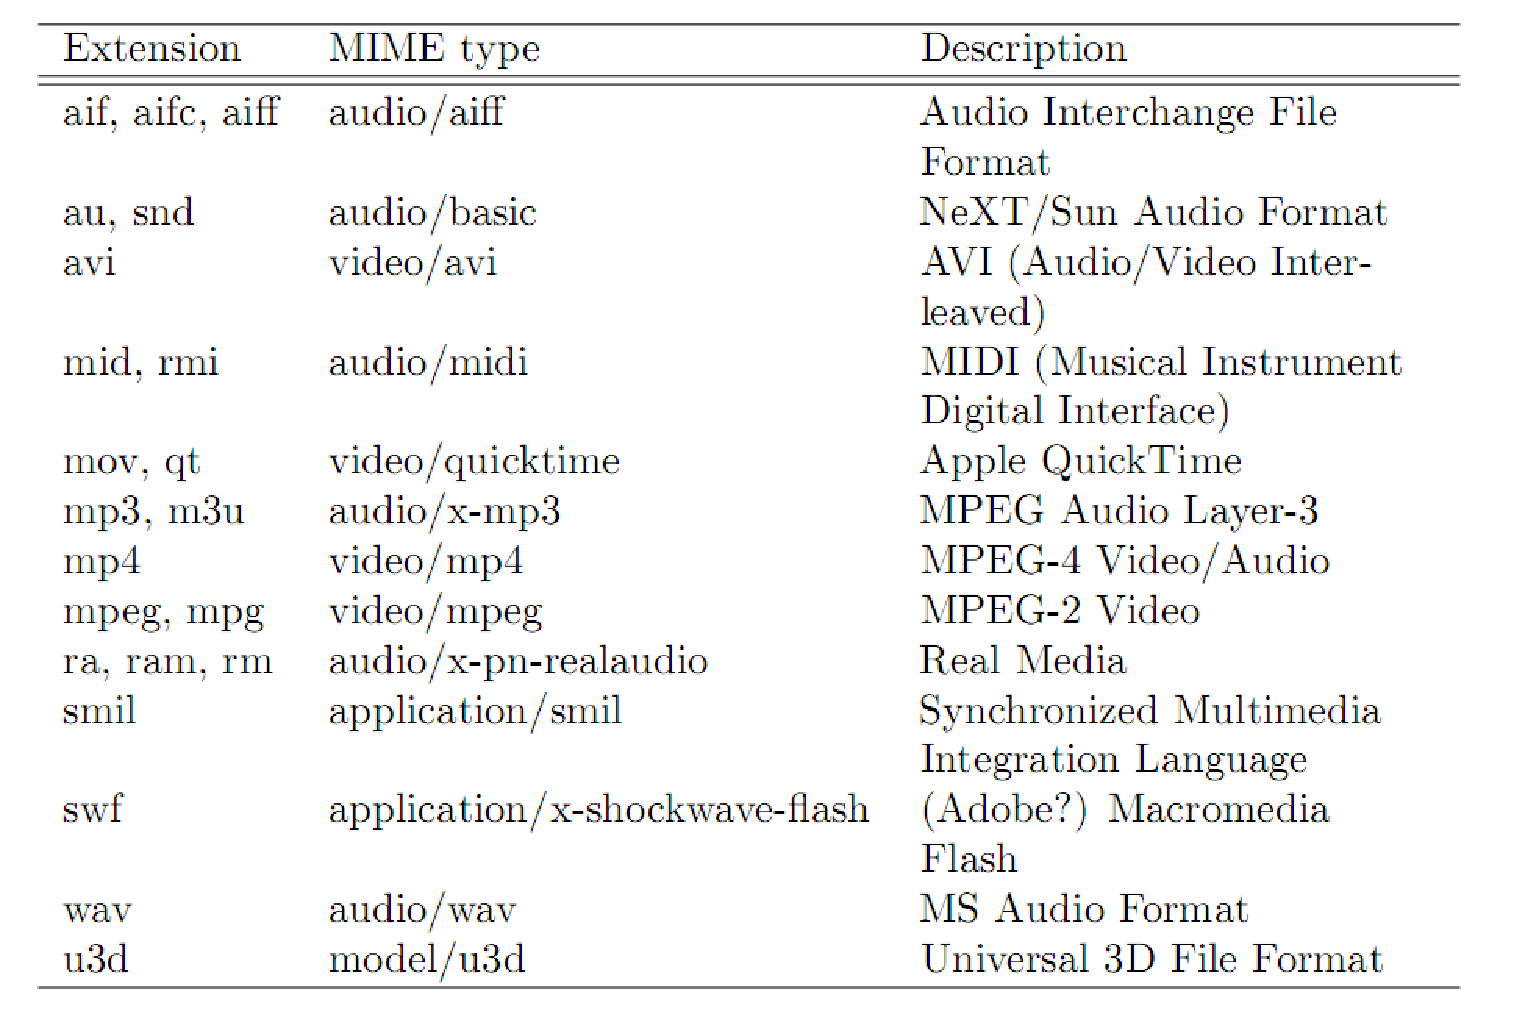
\includegraphics[width=14cm]{movie_format}\\

\end{table}

\subsection{attachfile2 宏包}

\index{命令!\verb$\textattachfile$}
\index{宏包!attachfile}
如\ref{movie_attach}所示双击在新文件中打开,注意如果在福昕阅读器中,
文件放在子文件夹内会读不出来反斜杠 \textcolor[rgb]{1.00,0.00,0.00}{/} 字符而不能播放,
AdobeReder 则没有问题,另外如果双击后无法打开 swf 文件,可能是播放器没有关联 swf 文件,可用 kmplayer 关联 swf 格式。
 \begin{shaded}
 \begin{Verbatim}
 \textattachfile{文件名}
 {\includegraphics[width=10cm]{封面}}
 \end{Verbatim}
 \end{shaded}

\begin{figure}[ht]
  \centering
\textattachfile{vim.swf}{
\includegraphics[width=10cm]{VIM.pdf}} \\
 \caption{attachfile 视频播放}\label{movie_attach}
\end{figure}
~\\


\begin{cmd}[label=attachfile2 使用样例代码]
\hyperlink{symbols}{\color{blue}\uline{\LaTeX 常用符号}}
\hypertarget{symbols}{\textcolor[rgb]
{0.00,0.00,1.00}{双击下面图标打开文档}}
\normalcolor
~\\[0.3cm]
\begin{center}
\fbox{
\textattachfile{appendix/symbols.pdf} %这里加入所添加的附件
{\parbox[b][4cm][c]{3cm}{ \color{blue} symbols \\\LaTeX 常用符号}}
}
\end{center}
\end{cmd}

效果见下一页:
\hyperlink{symbols}{\color{blue}\uline{\LaTeX 常用符号}}
\clearpage
\hypertarget{symbols}{\textcolor[rgb]
{0.00,0.00,1.00}{双击下面图标打开文档}}

\begin{center}
\fbox{
\textattachfile{symbols.pdf} %这里加入所添加的附件
{\parbox[b][4cm][c]{3cm}{ \color{blue} symbols \\\LaTeX 常用符号}}
}
\end{center}

\textcolor[rgb]{1.00,0.00,0.00}{注意:
attachfile2 支持 xelatex 模式,但不支持子文件夹,并与 hyperref 中选项有冲突,在导言区不能加入hyperref的 pdfauthor 等属性。}


%%%%%%%%%%%%%%%%%%%%%%%%%%%%%%%%%%%%%%%%%%%%%%%%%%%%%%%%%%%%%%%%%%%%
%\section{dir树}
\section{dirtree 结构图}
\subsection{dirtree 代码}
\index{宏包!dirtree}
\index{命令!\verb$\dirtree$}
使用 dirtree 宏包。如下图所示

\dirtree{%
.1 /.
.2 bin.
.2 home.
.3 jeancome.
.4 texmf.
.5 tex.
.6 latex.
.7 dirtree.
.3 jeancomeson.
.3 jeancomedaughter.
.2 usr.
.3 bin.
.3 games.
.4 fortunes.
.3 include.
.3 local.
.4 bin.
.4 share.
.5 texmf.
.6 fonts.
.6 metapost.
.6 tex.
.3 share.
}
对应代码如下:
\begin{lstlisting}
\dirtree{%
.1 /.
.2 bin.
.2 home.
.3 jeancome.
.4 texmf.
.5 tex.
.6 latex.
.7 dirtree.
.3 jeancomeson.
.3 jeancomedaughter.
.2 usr.
.3 bin.
.3 games.
.4 fortunes.
.3 include.
.3 local.
.4 bin.
.4 share.
.5 texmf.
.6 fonts.
.6 metapost.
.6 tex.
.3 share.
}
\end{lstlisting}




\subsection{dirtree 参数设计}
\begin{description}
  \item[DTstyle] 结点文字的属性
  \item[DTcomment] 右侧注释的内容
  \item[DTstylecomment] 右侧注释文字的属性
  \item[DTsetlength] 如下图所示
\begin{figure}[H]
  \centering
  % Requires \usepackage{graphicx}
  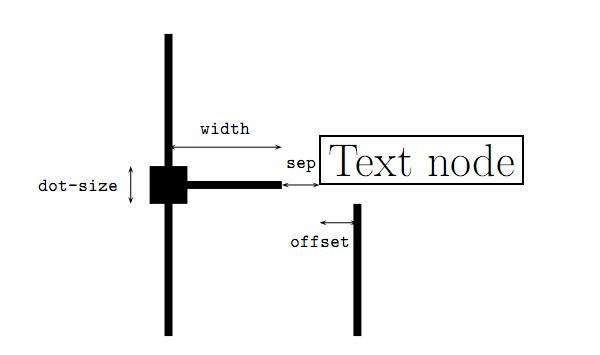
\includegraphics[width=10cm]{dirtree_length}\\
  \caption{dirtree 长度设置}\label{dirtree_length}
\end{figure}

\begin{cmd}[label= 长度设置命令]
    \DTsetlength{offset}{width}{sep}{rule-width}{dot-size}
默认值如下:
• offset=0.2em
• width=1em
• sep=0.2em
• rule-width=0.4pt
• dot-size=1.6pt
\end{cmd}
  \item[DTbaselineskip] 基线设置

\begin{cmd}[label= 基线设置命令]
\setlength{\DTbaselineskip}{20pt}
\DTsetlength{1em}{3em}{0.1em}{1pt}{4pt}
\end{cmd}
\end{description}

\renewcommand*\DTstylecomment{\rmfamily\color{green}\textsc}
\renewcommand*\DTstyle{\ttfamily\textcolor{red}}
\dirtree{%
.1 /.
.2 bin.
.2 home.
.3 jeancome.
.4 texmf.
.5 tex.
.3 jeancomeson\DTcomment{Guillaume}.
.3 jeancomedaughter\DTcomment{Mathilde}.
.2 usr.
.3 bin.
}


\lstset{language=[LaTeX]TeX}
\begin{lstlisting}
\dirtree{%
.1 /.
.2 bin.
.2 home.
.3 jeancome.
.4 texmf.
.5 tex.
.3 jeancomeson\DTcomment{Guillaume}.
.3 jeancomedaughter\DTcomment{Mathilde}.
.2 usr.
.3 bin.
}
\end{lstlisting}


\dirtree{%
.1 /.
.2 bin\ldots{}\begin{minipage}[t]{5cm}
This directory hold sexecutable files (binary
files or link on binary files){.}
\end{minipage}.
.2 home\ldots{}\begin{minipage}[t]{5cm}
jeancome\\
guillaume\\
mathilde\\
\end{minipage}.
.4 texmf.
}

\begin{lstlisting}

\dirtree{%
.1 /.
.2 bin\ldots{}\begin{minipage}[t]{5cm}
This directory hold sexecutable files (binary
files or link on binary files){.}
\end{minipage}.
.2 home\ldots{}\begin{minipage}[t]{5cm}
jeancome\\
guillaume\\
mathilde\\
\end{minipage}.
.4 texmf.
}
\end{lstlisting}


%%%%%%%%%%%%%%%%%%%%%%%%%%%%%%%%%%%%%%%%%%%%%%%%%%%%%%%%%%%%%%%%%%%%
%\section{bardiag树}
\section{bardiag 柱状图}
\index{宏包!bardiag}
\index{命令!\verb$\bardiag$}
\index{命令!\verb$\betweenticks$}
\subsection{bardiag 代码}
\renewcommand{\betweenticks}{50}
\bardiagrambegin{9.5}{200}{2cm}{1}{2}{1cm}{0.05cm}
\drawlevellines
\baritem{1998}{120}{green}
\baritem{1999}{123}{red}
\baritem{2000}{147}{yellow}
\baritem{2001}{176}{green}
\baritem{2002}{132}{red}
\bardiagramend{{\large Year}}{{\large Income}}

\lstset{language={[LaTeX]TeX}}
\begin{lstlisting}
\renewcommand{\betweenticks}{50}
\bardiagrambegin{9.5}{200}{2cm}{1}{2}{1cm}{0.05cm}
\drawlevellines
\baritem{1998}{120}{green}
\baritem{1999}{123}{red}
\baritem{2000}{147}{yellow}
\baritem{2001}{176}{green}
\baritem{2002}{132}{red}
\bardiagramend{{\large Year}}{{\large Income}}
\end{lstlisting}

\subsection{bardiag 参数设计}
\begin{figure}[H]
  \centering
  % Requires \usepackage{graphicx}
  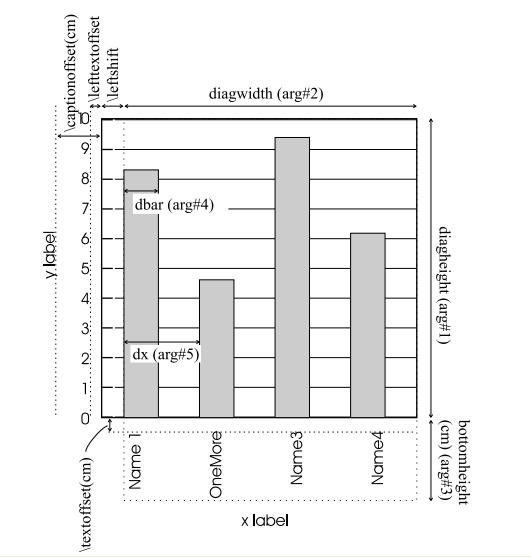
\includegraphics[width=14cm]{bardiag_set}\\
  \caption{bardiag 参数设计}\label{bardiag_set}
\end{figure}

%%%%%%%%%%%%%%%%%%%%%%%%%%%%%%%%%%%%%%%%%%%%%%%%%%%%%%%%%%%%%%%%%%%%
%\section{公式}
\section{公式}
常用 amsmath 宏包,用 texfriend 输入字符可自动加宏包。

\subsection{单行公式}
\index{命令!\verb$\($}
\index{命令!\verb$\[$}
\index{命令!\$}
\index{命令!\$\$}
\begin{Verbatim}[formatcom=\color{grass},frame=single,numbers=left]
$公式$:行内公式
\(公式\)
$$公式$$:行间公式
\end{Verbatim}

\subsection{多行公式}
\index{环境!equation}
\index{环境!gather}
单个公式编号可在 equation 环境内加入 split 环境,每个公式对应一编号用 gather 环境,默认居中对齐。
\textcolor[rgb]{1.00,0.00,0.00}{注意环境之间不要留空行。}
\begin{Verbatim}[formatcom=\color{grass},frame=single]
无标号
\[公式\]
equation 为单个公式
\begin{equation}
\begin{split}
  a^2 =c+4\\
  b^3 =e+6+b
\end{split}
\end{equation}
gather为多个公式,但在 split 环境里的公式只有一个编号
\begin{gather}
\begin{split}
  a^2 =c+4\\
  b^3 =e+6+b\\
c^2=3+c
\end{gather}
\end{Verbatim}

\begin{gather}
  a^2 =c+4\\
  b^3 =e+6+b\\
c^2=3+c
\end{gather}

\subsection{公式对齐}
\index{环境!align}
\index{环境!split}

单编号公式对齐可用 split 环境。\\
多编号公式对齐可用 align 环境。\\
align 环境还可以让多个公式同行显示对齐。
对齐符号为 \&,不写对齐符号默认右对齐,
用 split 后多行公式的公式编号居中,
在 gather 环境中用\verb$\notag$ 命令使本行公式不编号。
\begin{Verbatim}[formatcom=\color{grass},frame=single]
\begin{align}
  a^2 =c+4 \notag\\
  b^3 =e+6+b\\
  c^2=q+7+p+7
\end{align}
\end{Verbatim}

\begin{align}
  a^2 =c+4 \notag\\
  b^3 =e+6+b\\
  c^2=q+7+p+7
\end{align}

\subsection{大小自动调整括号}

\index{环境!matrix}
\index{环境!pmatrix}
\index{环境!bmatrix}	 
\index{环境!Bmatrix}	
\index{环境!vmatrix}	
\index{环境!Vmatrix}	
包括无框,小、中、大括号,单、双竖线。\\
\fbox{\parbox{12cm}{
\verbinput{body/fuhao.txt}}}
~\\
\par
\[\begin{matrix}
\begin{matrix} 1 & 2\\ 3 & 4 \end{matrix} &
\begin{pmatrix} 1 & 2\\ 3 & 4 \end{pmatrix} &
\begin{bmatrix} 1 & 2\\ 3 & 4 \end{bmatrix}\\[12pt]
\begin{Bmatrix} 1 & 2\\ 3 & 4 \end{Bmatrix} &
\begin{vmatrix} 1 & 2\\ 3 & 4 \end{vmatrix} &
\begin{Vmatrix} 1 & 2\\ 3 & 4 \end{Vmatrix}
\end{matrix}\]

\subsection{公式内加文本}
\index{命令!\verb$\text$}
\index{命令!\verb$\intertext$}
\begin{Verbatim}[formatcom=\color{grass},frame=single,numbers=left]
\text{文本}
行之间可用
\intertext{文本}
\end{Verbatim}

\subsection{公式自动编号}
\begin{Verbatim}[formatcom=\color{grass},frame=single,numbers=left]
\begin{equation}
可自动编号
\end{equation}
\begin{equation*}
不自动编号
\end{equation*}
\end{Verbatim}


%%%%%%%%%%%%%%%%%%%%%%%%%%%%%%%%%%%%%%%%%%%%%%%%%%%%%%%%%%%%%%%%%%%%
%\section{符号}
\section{符号}

\subsection{符号冲突}
多个符号宏包有冲突时,\LaTeX 以先引用的宏包为准。
有冲突的宏包如\ref{sym_clash}所示:

\begin{figure}[ht]
  \centering
  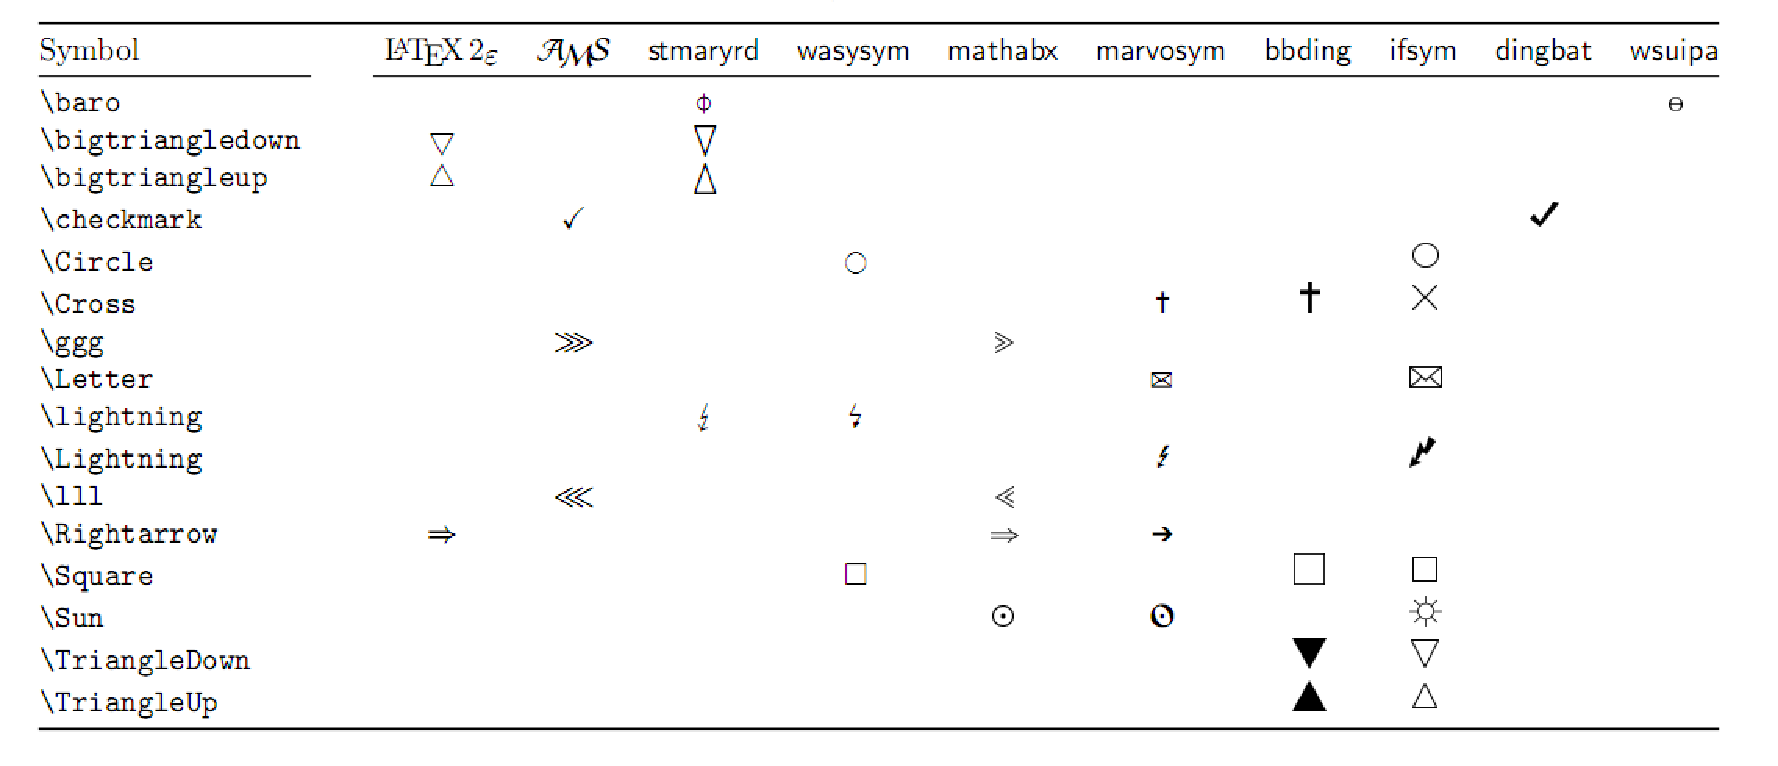
\includegraphics[width=14cm]{sym_clash}\\
   \caption{符号宏包冲突列表} \label{sym_clash}
\end{figure}

\index{宏包!amsmath}
\index{宏包!latexsym}
\index{宏包!dingbat}
\index{宏包!ifsym}
例如:本文档用以下宏包,其中 dingbat 宏包的 checkmark 与 AMS 有冲突,可直接按 Enter 键强行编译
或者找到宏包 dingbat.sty ,将其中 checkmark 的命令注释掉,再 texhash 一下即可
\begin{shaded}
\begin{verbatim}
\usepackage{amsmath,amsfonts,amssymb,gensymb} %
\usepackage{latexsym,bm,wasysym}        %公式符号
\usepackage[electronic]{ifsym} %电气符号
\usepackage{dingbat}
\end{verbatim}
\end{shaded}
到\verb| C:\ChinaTeX\texmf\tex\latex\dingbat| 打开 dingbat.sty 文件。注释掉以下命令。
\begin{shaded}
\begin{verbatim}
%\newcommand{\checkmark}{\dingbat@sym{'104}}
%wangfan注释,以免和 ams 冲突 2011.4.1
\end{verbatim}
\end{shaded}

\subsection{常用科技符号}
以下符号:
\begin{framed}
\Letter \quad \PulseHigh \quad \smallpencil \quad \largepencil \quad
\leftpointright\quad \Writinghand \quad \AC \quad \HF \quad \gluon \quad
\ohm \quad\degree \quad \celsius \quad \permil \quad

 $\mu \quad \alpha \quad\beta\quad\lambda\quad\nu\quad\omega \quad\xi\quad\rho\quad\tau\quad\phi\quad\eta\quad\theta$
\end{framed}
代码如下所示,可用 winedt 上的辅助公式输入栏,Greek 的数学符号要在数学模式下,在\verb|$...$|内,
可在winedt 内设置\verb|$...$|的快捷键,如设置 ALT+. 为 Insert$\Rightarrow$Latex中的\verb|$...$|快捷键,
可以选中一段文本按下 ALT+. 即可在文本周围加上\$:
\begin{shaded}
\begin{verbatim}
\Letter   \PulseHigh  \smallpencil  \largepencil
\leftpointright \Writinghand \AC   \HF  \gluon
 \ohm \degree  \celsius  \permil
 $\mu \alpha \beta \lambda \nu$
 $\omega \xi \rho \tau \phi \eta \theta$
\end{verbatim}
\end{shaded}

注意 ifsym 宏包在用到相关符号时,引用时需加对应 electronic,weather,misc 等选项
脉冲符号、数码管数字和符号拼接方法如\ref{ifsym}所示:\\

\begin{figure}[htbp]
  \centering
  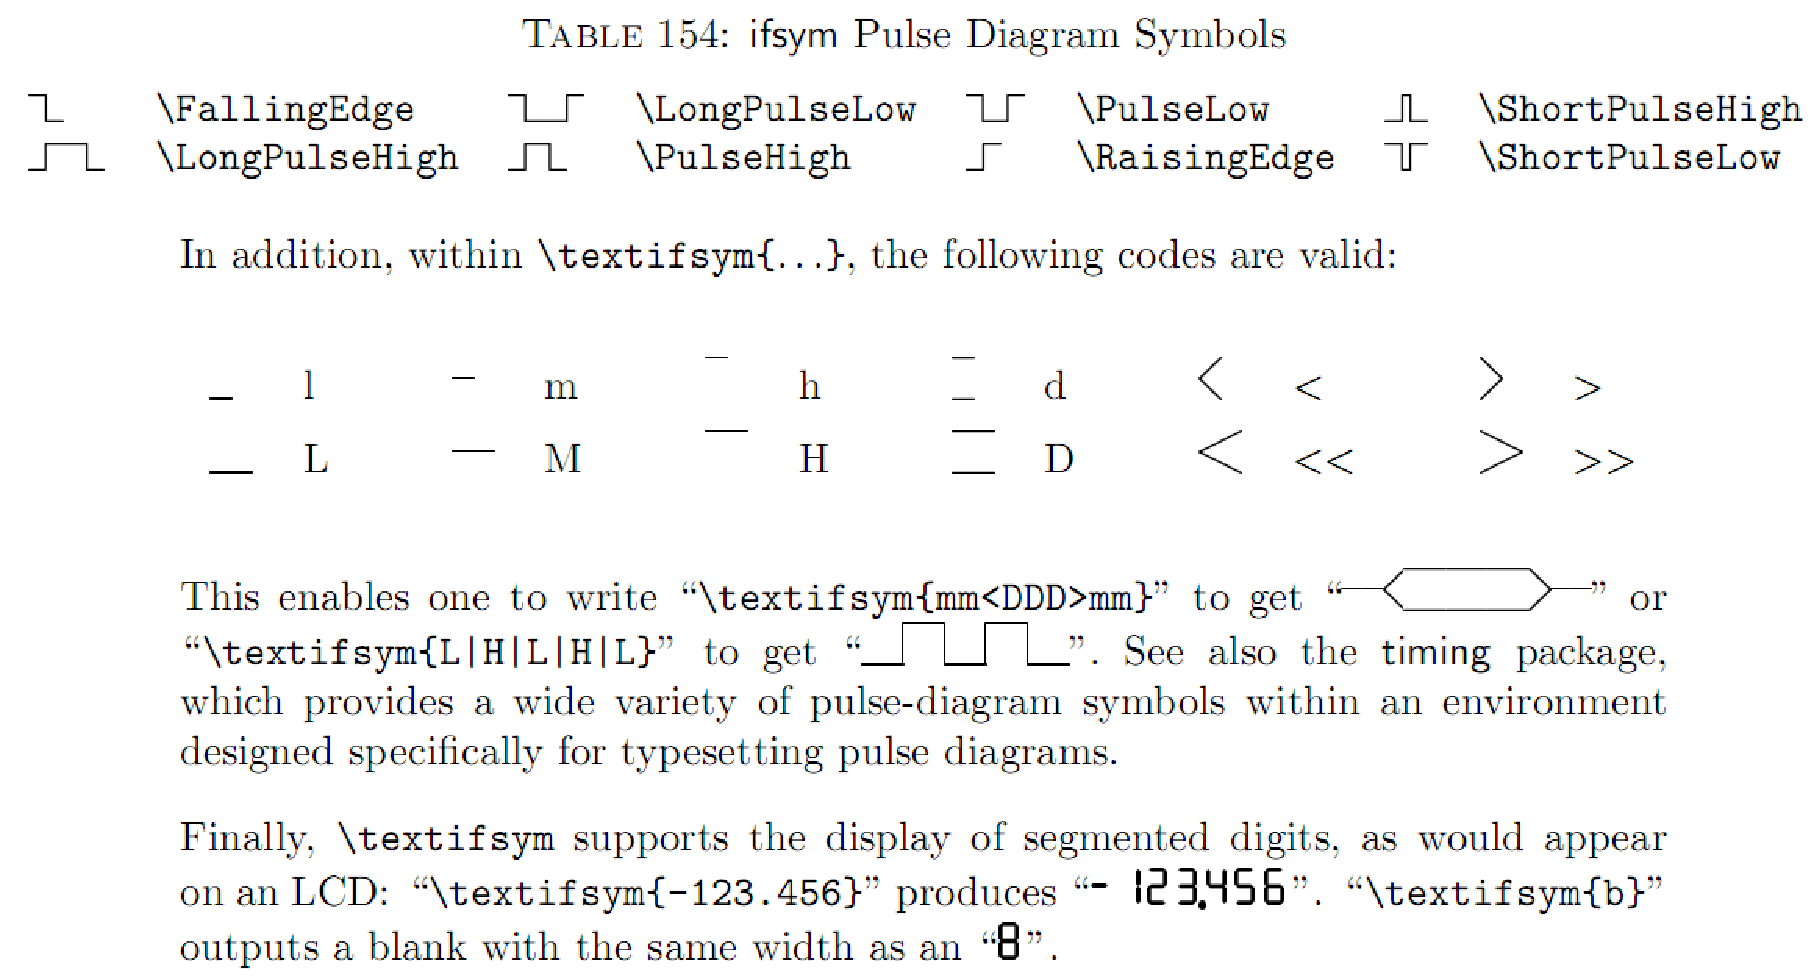
\includegraphics[width=14cm]{ifsym}\\
  \caption{脉冲符号及符号拼接}\label{ifsym}
\end{figure}



%%%%%%%%%%%%%%%%%%%%%%%%%%%%%%%%%%%%%%%%%%%%%%%%%%%%%%%%%%%%%%%%%%%%
%\section{索引}
\section{索引}
\index{命令!\verb$\makeindex$}
\index{命令!\verb$\printindex$}
\index{宏包!makeidx}

\subsection{默认宏包 makeidx}
用\textcolor[rgb]{1.00,0.00,0.00}{ makeindex 文件名 }处理 idx 后缀文件,可不写后缀。
\begin{shaded}
\begin{Verbatim}
\usepackage{makeidx}
\makeindex % 激活索引命令
\index{索引分类项!索引目标内容} % 放在对应的内容后
\printindex % 输出索引章节
\end{Verbatim}
\end{shaded}
注意:\\
\begin{enumerate}
  \item !、 \verb|@| 和 \verb$|$ 在 makeindex 里是命令字符。不能放在\verb|\index{...}|内
  \item \verb|\makeindex|注释掉则不产生索引。\index{命令!\verb$\makeinedex$}
  \item !为输入分类符,在后新建一条目,最多嵌套 3 层条目。
\end{enumerate}
效果如文末。


\subsection{xelatex 索引高级宏包 xeindex}

用法兼容makeidx宏包的命令。
\begin{lstlisting}[language={[LaTeX]TeX}]
\makeindex
\printindex
\index{entry}
`兼容以上命令`
`增加命令如下`
\IndexList*{}{list of entries}
\end{lstlisting}

%%%%%%%%%%%%%%%%%%%%%%%%%%%%%%%%%%%%%%%%%%%%%%%%%%%%%%%%%%%%%%%%%%%%
%\section{长度}
\section{长度设置}
\subsection{长度单位}
所有长度单位如下所示:\\
\begin{itemize}
  \item mm \item cm
  \item pt \item em \item ex
  \item sp \item bp \item pc
  \item cc \item dd \item in
  \item mu \item fil \item fill \item filll
\end{itemize}

最大长度不超过$2^{30}$sp=5758.3mm,主要用到长度如\ref{length}所示:\\
\begin{table}[htbp]
  \centering
  \caption{长度单位}\label{length}
\begin{tabular}{llllll}
  \toprule
  % after \\: \hline or \cline{col1-col2} \cline{col3-col4} ...
  单位 & 名称 & 说明 & 单位 & 名称 & 说明 \\
  \midrule
  mm & 毫米 & 1mm=2.845pt  & cm & 厘米 & 1mm=28.45pt \\
  pt & 点 & 1pt=0.351mm & em & em & 当前字体 M 的宽度 \\
  in & 英寸 & 1in=25.4mm=72.27pt & ex & ex & 当前字体 x 的高度 \\
  \bottomrule
\end{tabular}
\end{table}

\subsection{长度的设置}
可根据排版情况进行一定长度的伸长或缩短。弹性长度前不能相乘,否则长度变为 0 。\\

\index{命令!\verb$\fil$}
\index{命令!\verb$\hfil$}
\index{命令!\verb$\hfill$}
\index{命令!\verb$\vfil$}
\index{命令!\verb$\vfill$}
\index{命令!\verb$\quad$}
\index{命令!\verb$\qquad$}
\index{命令!\verb$\hspace$}
\index{命令!\verb$\vspace$}
\index{命令!\verb$\\[]$}
\index{命令!\verb$\newlength$}
\index{命令!\verb$\addvspace$}
\index{命令!plus }
\index{命令!minus}
\begin{table}[htbp]
  \centering
  \caption{长度设计}\label{length_design}
\rowcolors{1}{lightgray}{}
\begin{tabularx}{13cm}{p{5cm}X}
\toprule
2mm plus 0.2mm minus 0.3mm  &:表示长度根据排版需要在$2^{+0.2}_{-0.3}$mm内取值。\\
\verb|\fill \hfil \hfill \vfil \vfill| &: 从 0 到任意长\\
\verb|\hspace{长度}| &: 水平长度\\
\verb|\vspace{长度}| &: 竖直长度\\
\verb|\addvspce| &:  有条件的竖直长度\\
\verb|\\[长度]| &: 竖直长度\\
\verb|\quad \qquad| &: 1em,2em 长度\\
\verb|\newlength{..}| &: 新长度值\\
\verb|\phantom{字符串} \vphantom{字符串}| &: 生成字符串的总长(高)度\\
\bottomrule
\end{tabularx}
\end{table}


%%%%%%%%%%%%%%%%%%%%%%%%%%%%%%%%%%%%%%%%%%%%%%%%%%%%%%%%%%%%%%%%%%%%
%\section{页码 }
\section{页码、标号等计数器}
\subsection{计数器}
已有的计数器
\begin{itemize}
  \item part  \item section  \item subsection \item subsubsection
  \item chapter \item paragraph \item subparagraph \item page \item footnote
  \item equation
\end{itemize}
更改命令
\begin{latexcmd}
  \setcounter{计数器名称}{数字}  %给计数器赋值
  \addtocounter{计数器名称}{数字} %把指定值加入计数器
  \stepcounter{计数器名称} %指定计数器值加1,下属计数器清零
\end{latexcmd}

\subsection{最后页调用 LastPage}
lastpage 宏包使用,\verb|\pageref{LastPage}|命令即调用页码。

\subsection{指定页码调用 label}
本文档目录页下的页码调用代码如下:
\begin{latexcmd}
\label{page_menu} % 在目录页的最后一页后加入
\fancyfoot[C]{\textcolor[rgb]{0.00,0.59,0.00}{\thepage}/\pageref{LastPage}}

\end{latexcmd}
\subsection{页码重新设置格式}
\begin{latexcmd}
\pagenumbering{Roman}
\end{latexcmd}
\subsection{图号表号设置}
\begin{latexcmd}
\renewcommand*\figurename{}
\renewcommand*\tablename{}
\renewcommand\thefigure{图 \arabic{chapter}-\arabic{figure}~}
%将图号1.1改成1-1
\renewcommand\thetable{表 \arabic{chapter}-\arabic{table}~}
%将表号1.1改成1-1
\end{latexcmd}


%%%%%%%%%%%%%%%%%%%%%%%%%%%%%%%%%%%%%%%%%%%%%%%%%%%%%%%%%%%%%%%%%%%%
%\section{书签设置}
\section{书签设置}

\index{宏包!bookmark}
\index{命令!\verb$\bookmarksetup$}
可以对PDF书签的字体进行颜色等单独进行各种设置

\begin{lstlisting}[language={[LaTeX]TeX}]
  \usepackage[open,openlevel=1,atend]{bookmark}
  \bookmarksetup{italic,bold,color=blue}
  \bookmarksetup{bold=false,color={}}
\end{lstlisting}


%\section{PDF 注释}
%\section{PDF 注释}
%
%\index{宏包!pdfcomment}
%\index{命令!\verb$\pdffreetextcomment$}
%\index{命令!\verb$\pdftooltip$}
%可以对PDF中加入注释。但PDF的注释可以拖动,影响版式,推荐只使用pdftooltip这种不影响排版格式的注释。
%
%\begin{lstlisting}[language={[LaTeX]TeX}]
%  \usepackage{pdfcomment}
%  \pdftooltip[mathstyle]{ 原文 }{ 注释内容 } % mathstyle,disable 可选项
%\end{lstlisting}
%
%\pdftooltip{ 原文 }{ 注释内容 }


%%%%%%%%%%%%%%%%%%%%%%%%%%%%%%%%%%%%%%%%%%%%%%%%%%%%%%%%%%%%%%%%%%%%
%\section{自定义命令} % 与 listoftable 命令冲突
%\section{自定义命令}

\subsection{新建命令 newcommand def}
导言区加入:
\begin{lstlisting}[language={[LaTeX]TeX}]
\newcommand{\fengexian}[1]{
{\centering \makebox[\textwidth][s]{
\textcolor{red}{* * * * \mbox{#1} * * * *}}}}
\end{lstlisting}
定义中 [] 中数字表示变量的个数,在 \{\} 中 \#1 表示变量的位置
\begin{cmd}[label=用法]
\newcommand{\新函数}{新函数定义}
使用时:\新函数
如:\fengexian{我是分割线}
\end{cmd}
\fengexian{我是分割线}

\subsection{修改命令 renewcommand}


\subsection{自定义盒子 newsavebox}
\index{命令!\verb$\newsavebox$}
\index{命令!\verb$\savebox$}
\index{命令!\verb$\usebox$}
\index{命令!\verb$\sbox$}
\index{环境!lrbox}
其中 name 为自定义的名字,用以下代码可以直接用\verb|\usebox{\name}|来节省代码量。排版时 \TeX 只按盒子大小安排空间,若盒子里内容多出盒子空间,会导致与外部内容重叠,反之则出现大段空白。
\begin{lstlisting}
\newsavebox{\name} % 定义盒子名
\savebox( 宽度 , 高度 )[ 位置 ]{\name}{ 内容 } % 定义盒子内容
\sbox{\name}{ 内容 } % \savebox 的简略用法
\begin{lrbox}{\name} % 保存大段文本的盒子形式
    内容
\end{lrbox}
\usebox{\name}  % 引用盒子
\end{lstlisting}





%%%%%%%%%%%%%%%%%%%%%%%%%%%%%%%%%%%%%%%%%%%%%%%%%%%%%%%%%%%%%%%%%%%%%
%%\section{编译技巧}
\section{编译技巧}
节省时间
\subsection{注释一段文字}
在前加 \% 号,或在首尾加以下代码:
\begin{shaded}
\begin{Verbatim}
\iffalse
被注释的代码
\fi
\end{Verbatim}
\end{shaded}

\subsection{编译当前一小段}
这样还可以检查语法错误。
\begin{enumerate}
  \item 选中要编译的\TeX 代码
  \item 选择 Accessories$\rightarrow$Compile Selected,(快捷键 CTRL+SHIFT+C或SHIFT+F9)
  \item 会弹出 \LaTeX 编译后的效果
\end{enumerate}
\color{red}
当只想看新增部分的效果和查看新写的代码是否能编译通过时,这个命令十分好用,还可以在主界面选中几个章节如下所示:
\begin{shaded}
\begin{Verbatim}
%\bookmarksetup{bold,color=grass}
\chapter{\LaTeX 设计备忘}
\bookmarksetup{bold=false,color={}}
\thispagestyle{fancy}
\fancyhead[ER]{\song\wuhao\leftmark}\fancyhead[OL]{\song\wuhao\rightmark}
\fancyhead[EL]{\song\wuhao\rightmark}\fancyhead[OR]{\song\wuhao\leftmark}



~\\[9cm]
\begin{flushright}
\kai\xiaosi
\textcolor[rgb]{0.00,0.50,0.00}{
天下之事\\
其得之不难,则失之必易\\
其积之不久,则其发之必不宏\\
- - 王阳明}
\end{flushright}

%%%%%%%%%%%%%%%%%%%%%%%%%%%%%%%%%%%%%%%%%%%%%%%%%%%%%%%%%%%%%%%%%%%%

%\section{封面格式}
\include{body/title}


%\section{封面格式}
\include{body/multicol}

%%%%%%%%%%%%%%%%%%%%%%%%%%%%%%%%%%%%%%%%%%%%%%%%%%%%%%%%%%%%%%%%%%%%
%\section{版式设计}
\include{body/style}


%%%%%%%%%%%%%%%%%%%%%%%%%%%%%%%%%%%%%%%%%%%%%%%%%%%%%%%%%%%%%%%%%%%%

%\section{字体形式}
\include{body/char}


%%%%%%%%%%%%%%%%%%%%%%%%%%%%%%%%%%%%%%%%%%%%%%%%%%%%%%%%%%%%%%%%%%%%

%\section{代码}
\include{body/code}


%%%%%%%%%%%%%%%%%%%%%%%%%%%%%%%%%%%%%%%%%%%%%%%%%%%%%%%%%%%%%%%%%%%%

%\section{表格}
\include{body/table}



%%%%%%%%%%%%%%%%%%%%%%%%%%%%%%%%%%%%%%%%%%%%%%%%%%%%%%%%%%%%%%%%%%%%

%\section{图形}
\include{body/figure}

%%%%%%%%%%%%%%%%%%%%%%%%%%%%%%%%%%%%%%%%%%%%%%%%%%%%%%%%%%%%


%\section{合并PDF}
\include{body/pdf}

%%%%%%%%%%%%%%%%%%%%%%%%%%%%%%%%%%%%%%%%%%%%%%%%%%%%%%%%%%%%%%%%%%%%
%\section{环境}
\include{body/environment}



%%%%%%%%%%%%%%%%%%%%%%%%%%%%%%%%%%%%%%%%%%%%%%%%%%%%%%%%%%%%%%%%%%%%

%\section{参考文献}
\include{body/reference}

%%%%%%%%%%%%%%%%%%%%%%%%%%%%%%%%%%%%%%%%%%%%%%%%%%%%%%%%%%%%%%%%%%%%

%\section{超链接 href}
\include{body/hyperref}


%%%%%%%%%%%%%%%%%%%%%%%%%%%%%%%%%%%%%%%%%%%%%%%%%%%%%%%%%%%%%%%%%%%%

%\section{下划线 ulem}
\include{body/underline}

%%%%%%%%%%%%%%%%%%%%%%%%%%%%%%%%%%%%%%%%%%%%%%%%%%%%%%%%%%%%%%%%%%%%

%\section{脚注}
\include{body/footnote}

%%%%%%%%%%%%%%%%%%%%%%%%%%%%%%%%%%%%%%%%%%%%%%%%%%%%%%%%%%%%%%%%%%%%

%\section{盒子}
\include{body/box}


%%%%%%%%%%%%%%%%%%%%%%%%%%%%%%%%%%%%%%%%%%%%%%%%%%%%%%%%%%%%%%%%%%%

%\section{行号}
\include{body/lineno}

%%%%%%%%%%%%%%%%%%%%%%%%%%%%%%%%%%%%%%%%%%%%%%%%%%%%%%%%%%%%%%%%%%%%
%\section{动画}
\include{body/move}

%%%%%%%%%%%%%%%%%%%%%%%%%%%%%%%%%%%%%%%%%%%%%%%%%%%%%%%%%%%%%%%%%%%%
%\section{dir树}
\include{body/dirtree}

%%%%%%%%%%%%%%%%%%%%%%%%%%%%%%%%%%%%%%%%%%%%%%%%%%%%%%%%%%%%%%%%%%%%
%\section{bardiag树}
\include{body/bardiag}
%%%%%%%%%%%%%%%%%%%%%%%%%%%%%%%%%%%%%%%%%%%%%%%%%%%%%%%%%%%%%%%%%%%%
%\section{公式}
\include{body/math}

%%%%%%%%%%%%%%%%%%%%%%%%%%%%%%%%%%%%%%%%%%%%%%%%%%%%%%%%%%%%%%%%%%%%
%\section{符号}
\include{body/sym}

%%%%%%%%%%%%%%%%%%%%%%%%%%%%%%%%%%%%%%%%%%%%%%%%%%%%%%%%%%%%%%%%%%%%
%\section{索引}
\include{body/index}

%%%%%%%%%%%%%%%%%%%%%%%%%%%%%%%%%%%%%%%%%%%%%%%%%%%%%%%%%%%%%%%%%%%%
%\section{长度}
\include{body/length}

%%%%%%%%%%%%%%%%%%%%%%%%%%%%%%%%%%%%%%%%%%%%%%%%%%%%%%%%%%%%%%%%%%%%
%\section{页码 }
\include{body/page}

%%%%%%%%%%%%%%%%%%%%%%%%%%%%%%%%%%%%%%%%%%%%%%%%%%%%%%%%%%%%%%%%%%%%
%\section{书签设置}
\include{body/bookmark}

%\section{PDF 注释}
\include{body/pdfcomment}

%%%%%%%%%%%%%%%%%%%%%%%%%%%%%%%%%%%%%%%%%%%%%%%%%%%%%%%%%%%%%%%%%%%%
%\section{自定义命令} % 与 listoftable 命令冲突
%\include{body/newcommand}




%%%%%%%%%%%%%%%%%%%%%%%%%%%%%%%%%%%%%%%%%%%%%%%%%%%%%%%%%%%%%%%%%%%%%
%%\section{编译技巧}
\include{body/compile}


\renewcommand{\notesname}{本章注释}
\theendnotes
\setcounter{endnote}{0}
\clearpage
       %LATEX文档设计
%\bookmarksetup{bold,color=grass}
\chapter{绘图  Asymptote}
\bookmarksetup{bold=false,color={}}
\thispagestyle{fancy}

~\\[9cm]
\begin{flushright}
\kai\xiaosi
\textcolor[rgb]{0.00,0.50,0.00}{
所谓一流的才智\\
就是能够在心中怀有两种相互对立思维的同时\\
又能保持正常运作的能力\\
- - F.Z.Fitzgeraid\footnote{F.z.菲茨杰拉德:美国作家}}
\end{flushright}
\clearpage

优点:可画真 3D 图,在PDF中查看真 3D 是一种享受,\textcolor[rgb]{0.00,0.00,1.00}{可单独输出各种格式(png,eps)的文件\footnote{方便转换到 word 文档}};用 emacs 编辑可即时显示很爽。

%%%%%%%%%%%%%%%% 语法特点 %%%%%%%%%%%%%%%%%%%%%%
\section{Asymptote使用备注}

Asymptote 的编程命令与 C 和 C++ 一样,
以分号结束,中间的空白和换行不计。
注释符号为
//
和
/*
$\textellipsis$
*/

命令参数\\
\begin{Verbatim}[formatcom=\color{grass},frame=single,numbers=left]
//代码编译输出,默认输出eps格式,png 格式有的不是矢量图。
asy *.asy
asy -f pdf *.asy
asy -f png *.asy
asy -f eps *.asy
\end{Verbatim}

\begin{Verbatim}[formatcom=\color{grass},frame=single]
//可以在代码中加入选项设置代码,减少命令行命令
settings.outformat="pdf";
settings.tex="pdflatex";
setting.render=4;
//rend=4使生成的3D图形可被任意PDF阅读器查看封面
\end{Verbatim}

尽量不用中文,或只在注释中用中文,中文前后用逃逸字符框住,这样可以直接在 tex 文件中用 \verb|\lstinputlisting{文件路径}|来引用代码。

因为 PDFLATEX 编译后经常会出现将上面与下面截掉一小部分的情况,建议在绘制之前确定好高度,
在图的左侧开始处绘制出一条同底色的略大于原图高度的线条,防止截去正图中的部分。见\ref{code_automata}

\section{配置文件}
\begin{itemize}

  \item 使用 EMACS 编辑器,将 Asymptote 加入到.emacs 中,用 C-c C-c 就可以直接查看 EPS 编译后的文件了。
\scriptsize
\lstset{%extendedchars=false,% 解决中文跨页出错的问题;对 xetex 无用
basicstyle={\ttfamily},
numbersep=5pt}
\begin{lstlisting}[language={Lisp}]
;;asy`绘图设置`
(add-to-list 'load-path "C:/Program Files/Asymptote")
;;(add-to-list 'load-path "/usr/local/share/asymptote");;linux`路径设置`
(autoload 'asy-mode "asy-mode.el" "Asymptote major mode." t)
(autoload 'lasy-mode "asy-mode.el" "hybrid Asymptote/Latex major mode." t)
(autoload 'asy-insinuate-latex "asy-mode.el" "Asymptote insinuate LaTeX." t)
(add-to-list 'auto-mode-alist '("\\.asy$" . asy-mode))
\end{lstlisting}
\xiaosi

  \item 在 \verb$C:\Documents and Settings\Administrator\.asy$ 里新建 config.asy 文件,把应用到的软件路径加入进去:
\scriptsize
\begin{lstlisting}
import settings;
gs="D:\Program Files\gs\gs9.05\bin\gswin32c.exe";
psviewer="D:\Program Files\Ghostgum\gsview\gsview32.exe";
pdfviewer="D:\Program Files\Adobe\Acrobat 9.0\Acrobat\Acrobat.exe";
python="D:\python26\python.exe";
\end{lstlisting}
\xiaosi

  \item 把 \verb|c:\Program Files\Asymptote|里的 asycolors.sty ,asymptote.sty,ocg.sty 和下载的 animate.sty,animfp.sty,movie15.sty 放到 TEX 路径 \verb$c:\ChinaTeX\texmf\tex\latex$ 新建一个 Asymptote 的文件夹,然后进入 DOS 环境,用 texhash 命令更新一下 tex 的宏包。将自定义宏包simplenode.asy 放在  \verb|c:\Program Files\Asymptote|里面。

  \item 在代码前加入 settings.tex="pdflatex"; 这样 EMACS 就调用 pdflatex 进行编译,生成 PDF 文件,否则默认生成 EPS 文件。
\end{itemize}


%%%%%%%%%%%%%%%% 绘图命令 %%%%%%%%%%%%%%%%%%%%%%
\include{body/asy_command}

%%%%%%%%%%%%%%%% 绘图命令 %%%%%%%%%%%%%%%%%%%%%%
\include{body/asy_example}
       %ASY绘图设计
\end{Verbatim}
\end{shaded}

选中这几个\footnote{前面的\%号应该去掉},就可以对第一章,第二章进行编译查看效果了,不过里面的超链接编号会从头开始。PDF 图片和其他附件不会显示。
\color{black}

\subsection{只编译几个章节}
\index{命令!\verb$\includeonly$}

\begin{itemize}
  \item 在导言区加上\fcolorbox{white}{lightyellow}{$\backslash$includeonly\{文件名1,文件名2,...\}}。
  \item 需全文编译时,将命令注释掉即可
\end{itemize}

\subsection{删除辅助文件}
两种方法
\begin{enumerate}
  \item 点击 winedt 的回收站图标,可以选择把 \LaTeX 生成的辅助文件删除,方便快捷。
  \item 将以下文本另存为 clean.bat 文件,放在源文件夹中,双击即可。\textcolor[rgb]{1.00,0.00,0.00}{清除的文件还包括子文件夹。}
\begin{shaded}
  \begin{Verbatim}
del *.aux /s
del *.bak /s
del *.log /s
del *.bbl /s
del *.dvi /s
del *.blg /s
del *.thm /s
del *.toc /s
del *.out /s
  \end{Verbatim}
\end{shaded}
\end{enumerate}




\clearpage



\renewcommand{\notesname}{本章注释}
\theendnotes
\setcounter{endnote}{0}
\clearpage
       %LATEX文档设计
\clearpage
\bookmarksetup{bold,color=grass}
\chapter{绘图  pgf/tikz/pgfplot}
\bookmarksetup{bold=false,color={}}
\thispagestyle{fancy}
~\\[9cm]
\begin{flushright}
\kai\xiaosi
\textcolor[rgb]{0.00,0.50,0.00}{
毋意、毋必、毋固、毋我\\
- - 论语}
\end{flushright}
\clearpage

    pgf 最大的优点是可以直接放在源码 tex 文件中,即可以编译预览,帅气的中文支持,可直接用 PDFLaTeX 和 \XeLaTeX 和文档一起编译(比 mp 和 asy 方便),无须另外设置,在图形环境里还可以同样调用 \LaTeX 命令(如 listings 等宏包很有用)。而且 pgf 作者为 beamer 包的作者 Till Tantau 可以很好地兼容 beamer 文件。下面为其应用手册简介。

    由于本人是电子工程师,要画各种电路图,程序流程图,时序图。所以选择以下几个作重点介绍。


\begin{center}
\begin{minipage}[b]{10cm}
\textattachfile{pgfmanual.pdf}{\textcolor[rgb]{0.00,0.00,1.00}
{\fcolorbox{white}{lightblue}{\parbox{4cm}{\centering \kai \textcolor[rgb]{1.00,1.00,1.00}{~\\[0.5cm]pgf 2.1 \\ 英文手册\\[3cm]}}}}}\quad
\textattachfile{pgfmanual-ch.pdf}{\textcolor[rgb]{0.00,0.00,1.00}
{\fcolorbox{white}{lightblue}{\parbox{4cm}{\centering \kai \textcolor[rgb]{1.00,1.00,1.00}{~\\[0.5cm]pgf 2.1 \\ 中文手册\\[3cm]}}}}}
\end{minipage}
\end{center}
\begin{center}
\begin{minipage}[b]{10cm}
\textattachfile{pgfplots.pdf}{\textcolor[rgb]{0.00,0.00,1.00}
{\fcolorbox{white}{lightblue}{\parbox{4cm}{\centering \kai \textcolor[rgb]{1.00,1.00,1.00}{~\\[0.5cm]pgfplot \\ 英文手册\\[3cm]}}}}}\quad
\textattachfile{pgfplotstable.pdf}{\textcolor[rgb]{0.00,0.00,1.00}
{\fcolorbox{white}{lightblue}{\parbox{4cm}{\centering \kai \textcolor[rgb]{1.00,1.00,1.00}{~\\[0.5cm]pgfplotstable \\ 英文手册\\[3cm]}}}}}
\end{minipage}
\end{center}

\begin{center}
\begin{minipage}[b]{10cm}
\textattachfile{circuitikzmanual.pdf}{\textcolor[rgb]{0.00,0.00,1.00}
{\fcolorbox{white}{lightblue}{\parbox{4cm}{\centering \kai \textcolor[rgb]{1.00,1.00,1.00}{~\\[0.5cm]circuitikz \\ 英文手册\\[3cm]}}}}}\quad
\textattachfile{tikz-timing.pdf}{\textcolor[rgb]{0.00,0.00,1.00}
{\fcolorbox{white}{lightblue}{\parbox{4cm}{\centering \kai \textcolor[rgb]{1.00,1.00,1.00}{~\\[0.5cm]tikz-timing \\ 英文手册\\[3cm]}}}}}
\end{minipage}
\end{center}


看效果吧:

\begin{tikzpicture}
  [scale=3,line cap=round,
   % Styles
   axes/.style=,
   important line/.style={very thick},
   information text/.style={rounded corners,fill=red!10,inner sep=1ex}]

  % Local definitions
  \def\costhirty{0.8660256}

  % Colors
  \colorlet{anglecolor}{green!50!black}
  \colorlet{sincolor}{red}
  \colorlet{tancolor}{orange!80!black}
  \colorlet{coscolor}{blue}

  % The graphic
  \draw[help lines,step=0.5cm] (-1.4,-1.4) grid (1.4,1.4);

  \draw (0,0) circle (1cm);

  \begin{scope}[axes]
    \draw[->] (-1.5,0) -- (1.5,0) node[right] {$x$};
    \draw[->] (0,-1.5) -- (0,1.5) node[above] {$y$};

    \foreach \x/\xtext in {-1, -.5/-\frac{1}{2}, 1}
      \draw[xshift=\x cm] (0pt,1pt) -- (0pt,-1pt) node[below,fill=white] {$\xtext$};

    \foreach \y/\ytext in {-1, -.5/-\frac{1}{2}, .5/\frac{1}{2}, 1}
      \draw[yshift=\y cm] (1pt,0pt) -- (-1pt,0pt) node[left,fill=white] {$\ytext$};
  \end{scope}

  \filldraw[fill=green!20,draw=anglecolor] (0,0) -- (3mm,0pt) arc(0:30:3mm);
  \draw (15:2mm) node[anglecolor] {$\alpha$};

  \draw[important line,sincolor]
    (30:1cm) -- node[left=1pt,fill=white] {$\sin \alpha$} +(0,-.5);

  \draw[important line,coscolor]
    (0,0) -- node[below=2pt,fill=white] {$\cos \alpha$} (\costhirty,0);

  \draw[important line,tancolor] (1,0) --
    node [right=1pt,fill=white]
    {
      $\displaystyle \tan \alpha \color{black}=
      \frac{{\color{sincolor}\sin \alpha}}{\color{coscolor}\cos \alpha}$
    } (intersection of 0,0--30:1cm and 1,0--1,1) coordinate (t);

  \draw (0,0) -- (t);

  \draw[xshift=1.85cm] node [right,text width=6cm,information text]
    {
      The {\color{anglecolor} angle $\alpha$} is $30^\circ$ in the
      example ($\pi/6$ in radians). The {\color{sincolor}sine of
        $\alpha$}, which is the height of the red line, is
      \[
      {\color{sincolor} \sin \alpha} = 1/2.
      \]
      By the Theorem of Pythagoras we have ${\color{coscolor}\cos^2 \alpha} +
      {\color{sincolor}\sin^2\alpha} =1$. Thus the length of the blue
      line, which is the {\color{coscolor}cosine of $\alpha$}, must be
      \[
      {\color{coscolor}\cos\alpha} = \sqrt{1 - 1/4} = \textstyle
      \frac{1}{2} \sqrt 3.
      \]%
      This shows that {\color{tancolor}$\tan \alpha$}, which is the
      height of the orange line, is
      \[
      {\color{tancolor}\tan\alpha} = \frac{{\color{sincolor}\sin
          \alpha}}{\color{coscolor}\cos \alpha} = 1/\sqrt 3.
      \]%
    };
\end{tikzpicture}


%%%%%%%%%%%%%%%%  %%%%%%%%%%%%%%%%%%%%%%
\section{tikz 使用方法}
注: \XeLaTeX 下的 shading 和 spy 宏包有问题,不能产生效果。
\subsection{调用宏包}
\subsection{调用环境}
\subsection{tikzset 绘图预定义}
可提前设置好颜色等设置和调用以前的模板。
\begin{itemize}
  \item \verb|\tikzset{...}|:在导言区或绘图前加入
  \item \verb|\begin{tikzpicture}[...]|;在 [] 中加入
\end{itemize}
\section{tikz 基本绘图命令}
\begin{itemize}
  \item tikz 是基于坐标系的,原点在当前左下角
  \item 每条绘图命令以分号结束
  \item 默认长度为1cm,可加可不加,shift 等其他命令必须加.
\end{itemize}


\subsection{绘图环境和绘图命令}
绘图环境,tikz 绘图的基本单元是路径 path,路径有点和连接方式两种基本元素,可以被画、填充、裁剪...。
点可以通过坐标或其他方式给出,连接方式有直线、曲线、弧线。


\begin{minipage}[c]{9cm}
\begin{cmd}[label= Path 的绘制命令]
\path[draw](1,1)--(2,2)--(3,1);
\path[draw,yshift=-2cm]%
(1,1)--(2,2)--(3,1)--cycle;
\path[draw,fill=green!20,yshift=-4cm]%
(1,1)--(2,2)--(3,1)--cycle;
\path[fill=green,yshift=-6cm]%
(1,1)--(2,2)--(3,1)--cycle;
\path[clip,draw,yshift=-8cm]%
(1,1)--(2,2)--(3,1)--cycle;
\path[fill=blue!50](2,1.7-8)circle(.8);
\end{tikzpicture}
\end{cmd}
\end{minipage}
\quad\quad
\begin{minipage}{3cm}
\begin{tikzpicture}
\path[draw](1,1)--(2,2)--(3,1);
\path[draw,yshift=-2cm]%
(1,1)--(2,2)--(3,1)--cycle;
\path[draw,fill=green!20,yshift=-4cm]%
(1,1)--(2,2)--(3,1)--cycle;
\path[fill=green,yshift=-6cm]%
(1,1)--(2,2)--(3,1)--cycle;
\path[clip,draw,yshift=-8cm]%
(1,1)--(2,2)--(3,1)--cycle;
\path[fill=blue!50](2,1.7-8)circle(.8);
\end{tikzpicture}
\end{minipage}

\begin{cmd}[label= Path 的缩写命令]
\draw=\path[draw]
\fill=\path[fill]
\clip=\path[clip]
\filldraw=\path[fill,draw]
\shade=\path[shade]
\end{cmd}
\begin{itemize}
  \item \verb|\tikz|或\verb|\begin{tikzpicture}| 开始绘制环境
   \item \verb|\draw| 和\verb|\filldraw| 等直接绘制命令。
    \item \verb|\foreach|  等控制绘制命令。
\end{itemize}


\subsection{绘制路径}
\begin{minipage}{2.5cm}
\begin{tikzpicture}[thick]
\draw (0,3) -- (3,3);
\draw[decorate,decoration=zigzag] (0,2.5) -- (3,2.5);
\draw[decorate,decoration=brace] (0,2) -- (3,2);
\draw[decorate,decoration=triangles] (0,1.5) -- (3,1.5);
\draw[decorate,decoration={coil,segment length=4pt}] (0,1) -- (3,1);
\draw[decorate,decoration={coil,aspect=0}] (0,.5) -- (3,.5);
\draw[decorate,decoration={expanding waves,angle=7}] (0,0) -- (3,0);
\end{tikzpicture}
\end{minipage}
\begin{minipage}{10cm}
\begin{lstlisting}
\begin{tikzpicture}[thick]
\draw (0,3) -- (3,3);
\draw[decorate,decoration=zigzag] (0,2.5) -- (3,2.5);
\draw[decorate,decoration=brace] (0,2) -- (3,2);
\draw[decorate,decoration=triangles] (0,1.5) -- (3,1.5);
\draw[decorate,decoration={coil,segment length=4pt}] (0,1) -- (3,1);
\draw[decorate,decoration={coil,aspect=0}] (0,.5) -- (3,.5);
\draw[decorate,decoration={expanding waves,angle=7}] (0,0) -- (3,0);
\end{tikzpicture}
\end{lstlisting}
\end{minipage}

\subsection{绘制结点和标注 node coordinate}
\begin{cmd}[label= node 添加标注用法]
\draw (x1,y1)--(x2,y2) node[anchor=方向]{标注文字}
方向有 east,north,west,south
\node[选项]at(x,y)[选项]{text}
text 为显示的文字
\node(标记)[选项]at(x,y)[选项]{text}
\coordinate[label=角度:标注](标记)at(x,y)
\end{cmd}
\section{输出 pdf,png,eps单独格式图片}


\subsection{ pdf 图形全部预览 preview}
在导言区加入 preview 宏包,可实现全部 tikz 环境的图形预览,每个图形一页。包括 circuitikz 和 tikz-timing 宏包环境。可单独建立一个tex文件以实现单独的PDF文件输出,PreviewBorder 内的参数表示图形与周围空白的间距。
\begin{cmd}
\usepackage[active,tightpage]{preview}
\PreviewEnvironment{tikzpicture}
\setlength\PreviewBorder{15pt}
\end{cmd}

\subsection{xelatex 设置单独输出 pdf}
在 winedt 设置中将 options$\rightarrow$Execution Mode$\rightarrow$Console Applications$\rightarrow$\XeLaTeX$\rightarrow$Executable 的值变成如下所示,加入 -shell-escape 参数的作用是使 \XeLaTeX 能递归调用自己来产生图片。pdflatex 同上所示。
\begin{cmd}
  xelatex.exe -shell-escape
\end{cmd}
\subsection{调用宏包及设置}
需要tikz,tikzlibrary 的 extern 包。
\begin{lstlisting}[language={[LaTeX]TeX}]
\usepackage{tikz}
\usetikzlibrary{external}
\tikzexternalize %activate!
\tikzset{external/system call={xelatex \tikzexternalcheckshellescape
-halt-on-error-interaction=batchmode -jobname "\image" "\texsource"}}
\tikzsetexternalprefix{figures/}% 设置图片保存路径
\tikzsetnextfilename{trees} % 紧跟下一幅图名
\tikzsetfigurename{subset_} % 重设默认图名重设可用 {} 限定范围
\tikzexternaldisable % 暂时取消
\tikzexternalenable % 重新使能
\end{lstlisting}
\subsection{external 宏包兼容性设置}
如果 \XeLaTeX 调用了 \verb|\def\pgfsysdriver{pgfsys-dvipdfmx.def}| 命令,会导致出错不能使用 external,如果要用 pdfpage 等宏包,需在导言区做以下更改引用相关宏包。
\begin{lstlisting}[language={[LaTeX]TeX}]
\usetikzlibrary{external}
\tikzifexternalizing{%
%don'tincludepackageXYZhere
}{%
\usepackage{pdfpages}
\usepackage{vmargin}
...
}%
\end{lstlisting}

\section{插入外部图片}

\begin{enumerate}
  \item 声明 \verb|\pgfdeclareimage[options]{image name}{filename}|
  \item 插入 \verb|pgfuseimage{image name}|
  \item 或用以下命令替代上述两个命令 \verb|\pgfimage[options]{filename}|
\end{enumerate}

\section{tikz-timing 时序图}
\tikzexternaldisable

\noindent\verb|\texttiming{HLZDZLH}|: \texttiming{HLZDZLH}\\
\verb|\texttiming[green,timing/initchar=L]{HLZDZLH}|: \texttiming[green,timing/initchar=L]{HLZDZLH}
\begin{figure}[H]
  \centering
\begin{tikztimingtable}
Clock 128\,MHz 0\degr & H 2C N(A1) 8{2C} N(A5) 3{2C} G\\
Clock 128\,MHz 90\degr & [C] 2{2C} N(A2) 8{2C} N(A6) 2{2C} C\\
Clock 128\,MHz 180\degr & C 2{2C} N(A3) 8{2C} N(A7) 2{2C} G\\
Clock 128\,MHz 270\degr & 3{2C} N(A4) 8{2C} N(A8) 2C C\\
Coarse Pulse & 3L 16H 6L \\
Coarse Pulse - Delayed 1 & 4L N(B2) 16H N(B6) 5L \\
Coarse Pulse - Delayed 2 & 5L N(B3) 16H N(B7) 4L \\
Coarse Pulse - Delayed 3 & 6L 16H 3L \\
\\
Final Pulse Set & 3L 16H N(B5) 6L \\
Final Pulse $\overline{\mbox{Reset}}$ & 6L N(B4) 16H 3L \\
Final Pulse & 3L N(B1) 19H N(B8) 3L \\
\extracode
\tablerules
\begin{pgfonlayer}{background}
\foreach \n in {1,...,8}
\draw [help lines] (A\n) -- (B\n);
\end{pgfonlayer}
\end{tikztimingtable}
 \caption{时序图pgf}\label{pgf_timing}
\end{figure}
\begin{lstlisting}
\begin{figure}[H]
  \centering
\begin{tikztimingtable}
Clock 128\,MHz 0\degr & H 2C N(A1) 8{2C} N(A5) 3{2C} G\\
Clock 128\,MHz 90\degr & [C] 2{2C} N(A2) 8{2C} N(A6) 2{2C} C\\
Clock 128\,MHz 180\degr & C 2{2C} N(A3) 8{2C} N(A7) 2{2C} G\\
Clock 128\,MHz 270\degr & 3{2C} N(A4) 8{2C} N(A8) 2C C\\
Coarse Pulse & 3L 16H 6L \\
Coarse Pulse - Delayed 1 & 4L N(B2) 16H N(B6) 5L \\
Coarse Pulse - Delayed 2 & 5L N(B3) 16H N(B7) 4L \\
Coarse Pulse - Delayed 3 & 6L 16H 3L \\
\\
Final Pulse Set & 3L 16H N(B5) 6L \\
Final Pulse $\overline{\mbox{Reset}}$ & 6L N(B4) 16H 3L \\
Final Pulse & 3L N(B1) 19H N(B8) 3L \\
\extracode
\tablerules
\begin{pgfonlayer}{background}
\foreach \n in {1,...,8}
\draw [help lines] (A\n) -- (B\n);
\end{pgfonlayer}
\end{tikztimingtable}
 \caption{`时序图`pgf}\label{pgf_timing}
\end{figure}
\end{lstlisting}

\tikzexternalenable

\section{pgf 流程图}

\subsection{预定义形状和节点}
设置好结点和图形,放在导言区。
\begin{lstlisting}
\tikzset{
passprocess/.style={
rectangle,
draw=blue,
minimum width=50pt,
minimum height=20pt,
font=\ttfamily,
text centered
},
startstop/.style={
rectangle,%
rounded corners=5pt,%
minimum width=50pt,
minimum height=20pt,
text centered,
fill=orange,
font=\ttfamily,
draw=red
},
decision/.style={
diamond,%
shape aspect=2,%aspect value is the ratio of width and height for diamond
draw=green,%the color of line
fill=lime,%filled color
font=\ttfamily,%set font
text centered%surely you know what it means
},%here is a
line/.style = {
draw,
->,
%shorten>=2pt,
thick
}}
\end{lstlisting}

\subsection{流程图的绘制}

\begin{cmd}[label=流程图命令]
\matrix [row sep=行距,column sep=列距]{节点定义代码} %节点行列分布
\node (节点序号) [节点类型] {节点内容} %节点内容设置
\begin{scope}[every path/.style=line] %节点连线设置
\path () -- () %竖线相连
\path () |- () %先竖再折
\path () -| () %先折再竖
\end{scope}
\end{cmd}

\begin{tikzpicture}
\matrix[row sep=5mm,column sep=5mm]
{
%First row:
\node (p1) [startstop] {开始};&\\
%Second row;
\node (p2) [passprocess] {问问题咯};&\\
%Third row:
\node (p31) [decision] {a你是大牛么:?};&
\node (p32) [passprocess] {b你才是大牛:};\\
%Fourth row:
&
\node (p4) [passprocess] {b你全家都是大牛:};\\
%Fifth row:
&
\node (p42) [passprocess] {b你家小狗都是大牛:};\\
%Sixth row:
\node (p5) [passprocess] {a当我什么也没说:};&\\
%Seventh row:
\node (p6) [startstop] {结束};&\\
};

\begin{scope}[every path/.style=line]
\path (p1) -- (p2);
\path (p2) -- (p31);
\path (p31) -- node [near start,above] {yes} (p32);
\path (p32) -- (p4);
\path (p4) -- (p42);
\path (p5) -- (p6);
\path (p42) |-(p5);%表示先竖后折, -|表示先折后竖
\path (p31) -- node [midway,left] {no} (p5);
\end{scope};
\draw[xshift=4.35cm] node [right,text width=7cm,information text]
    {\tiny
    \begin{lstlisting}[backgroundcolor={\color{red!10}}]
\begin{tikzpicture}
[information text/.style={rounded corners,
fill=red!10,inner sep=0ex}]
\matrix[row sep=5mm,column sep=5mm]
{
%First row:
\node (p1) [startstop] {`开始`};&\\
%Second row;
\node (p2) [passprocess] {`问问题咯`};&\\
%Third row:
\node (p31) [decision] {a`你是大牛么`:?};&
\node (p32) [passprocess] {b`你才是大牛`:};\\
%Fourth row:
&
\node (p4) [passprocess] {b`你全家都是大牛`:};\\
%Fifth row:
&
\node (p42) [passprocess] {b`你家小狗都是大牛`:};\\
%Sixth row:
\node (p5) [passprocess] {a`当我什么也没说`:};&\\
%Seventh row:
\node (p6) [startstop] {`结束`};&\\
};

\begin{scope}[every path/.style=line]
\path (p1) -- (p2);
\path (p2) -- (p31);
\path (p31) -- node [near start,above] {yes} (p32);
\path (p32) -- (p4);
\path (p4) -- (p42);
\path (p5) -- (p6);
\path (p42) |-(p5);%`表示先竖后折, -|表示先折后竖`
\path (p31) -- node [midway,left] {no} (p5);
\end{scope};
};
\end{tikzpicture}
    \end{lstlisting}
      };
\end{tikzpicture}


\section{pgf 状态机}

\begin{minipage}{5cm}
\begin{tikzpicture}[shorten >=1pt,node distance=2cm,on grid,auto]
\draw[help lines] (0,0) grid (3,2);
\node[state,initial] (q_0) {$q_0$};
\node[state] (q_1) [above right=of q_0] {$q_1$};
\node[state] (q_2) [below right=of q_0] {$q_2$};
\node[state,accepting](q_3) [below right=of q_1] {$q_3$};
\path[->] (q_0) edge node {0} (q_1)
edge node [swap] {1} (q_2)
(q_1) edge node {1} (q_3)
edge [loop above] node {0} ()
(q_2) edge node [swap] {0} (q_3)
edge [loop below] node {1} ();
\end{tikzpicture}
\end{minipage}
\begin{minipage}{10cm}
\begin{lstlisting}
\begin{tikzpicture}
[shorten >=1pt,node distance=2cm,on grid,auto]
\draw[help lines] (0,0) grid (3,2);
\node[state,initial] (q_0) {$q_0$};
\node[state] (q_1) [above right=of q_0] {$q_1$};
\node[state] (q_2) [below right=of q_0] {$q_2$};
\node[state,accepting](q_3) [below right=of q_1] {$q_3$};
\path[->] (q_0) edge node {0} (q_1)
edge node [swap] {1} (q_2)
(q_1) edge node {1} (q_3)
edge [loop above] node {0} ()
(q_2) edge node [swap] {0} (q_3)
edge [loop below] node {1} ();
\end{tikzpicture}
\end{lstlisting}
\end{minipage}

\begin{tikzpicture}[->,>=stealth',shorten >=1pt,auto,node distance=2.8cm,on grid,semithick,
                    every state/.style={fill=red,draw=none,circular drop shadow,text=white}]

  \node[initial,state] (A)                    {$q_a$};
  \node[state]         (B) [above right=of A] {$q_b$};
  \node[state]         (D) [below right=of A] {$q_d$};
  \node[state]         (C) [below right=of B] {$q_c$};
  \node[state]         (E) [below=of D]       {$q_e$};

  \path (A) edge              node {0,1,L} (B)
            edge              node {1,1,R} (C)
        (B) edge [loop above] node {1,1,L} (B)
            edge              node {0,1,L} (C)
        (C) edge              node {0,1,L} (D)
            edge [bend left]  node {1,0,R} (E)
        (D) edge [loop below] node {1,1,R} (D)
            edge              node {0,1,R} (A)
        (E) edge [bend left]  node {1,0,R} (A);

   \node [right=0.2cm,text width=8cm] at (C)
   {\scriptsize
\begin{lstlisting}[language={verilog},backgroundcolor={\color{red!10}}]
\begin{tikzpicture}
[->,>=stealth',shorten >=1pt,auto,
node distance=2.8cm,on grid,semithick,
every state/.style={fill=red,draw=none,
circular drop shadow,text=white}]
  \node[initial,state] (A)                    {$q_a$};
  \node[state]         (B) [above right=of A] {$q_b$};
  \node[state]         (D) [below right=of A] {$q_d$};
  \node[state]         (C) [below right=of B] {$q_c$};
  \node[state]         (E) [below=of D]       {$q_e$};

  \path (A) edge              node {0,1,L} (B)
            edge              node {1,1,R} (C)
        (B) edge [loop above] node {1,1,L} (B)
            edge              node {0,1,L} (C)
        (C) edge              node {0,1,L} (D)
            edge [bend left]  node {1,0,R} (E)
        (D) edge [loop below] node {1,1,R} (D)
            edge              node {0,1,R} (A)
        (E) edge [bend left]  node {1,0,R} (A);
\end{tikzpicture}
\end{lstlisting}
   };
\end{tikzpicture}


\section{pgfplot 坐标图}

\begin{tikzpicture}
[every entity/.style={draw=blue!50,fill=blue!20,thick}]
\node[entity] (sheep) {Sheep};
\node[entity] (genome) [right=of sheep] {Genome};
\end{tikzpicture}

\begin{tikzpicture}
\begin{axis}[
xlabel=Cost,
ylabel=Error]
\addplot[color=red,mark=x] coordinates {
(2,-2.8559703)
(3,-3.5301677)
(4,-4.3050655)
(5,-5.1413136)
(6,-6.0322865)
(7,-6.9675052)
(8,-7.9377747)
};
\end{axis}
\end{tikzpicture}


\section{pgf 矩阵图}

\begin{minipage}{3cm}
\begin{tikzpicture}
\matrix (magic) [matrix of nodes]
{
8 & 1 & 6 \\
3 & 5 & 7 \\
4 & 9 & 2 \\
};
\draw[thick,red,->] (magic-1-1) |- (magic-2-3);
\end{tikzpicture}

\begin{tikzpicture}
\matrix [matrix of nodes]
{
8 &[1cm] 1 &[3mm] |[red]| 6 \\
3 & 5 & |[red]| 7 \\
4 & 9 & 2 \\
};
\end{tikzpicture}

\begin{tikzpicture}
\matrix [matrix of math nodes,nodes={circle,draw},nodes in empty cells]
{
a_8 & & a_6 \\
a_3 & & a_7 \\
a_4 & a_9 & \\
};
\end{tikzpicture}
\end{minipage}
%%%%%%%%%%%%%%%%%%%%%%%%%%%%%%%%%%%
\begin{minipage}{10cm}
\scriptsize
\begin{lstlisting}
\begin{tikzpicture}
\matrix (magic) [matrix of nodes]
{
8 & 1 & 6 \\
3 & 5 & 7 \\
4 & 9 & 2 \\
};
\draw[thick,red,->] (magic-1-1) |- (magic-2-3);
\end{tikzpicture}

\begin{tikzpicture}
\matrix [matrix of nodes]
{
8 &[1cm] 1 &[3mm] |[red]| 6 \\
3 & 5 & |[red]| 7 \\
4 & 9 & 2 \\
};
\end{tikzpicture}

\begin{tikzpicture}
\matrix
[matrix of math nodes,nodes={circle,draw},nodes in empty cells]
{
a_8 & & a_6 \\
a_3 & & a_7 \\
a_4 & a_9 & \\
};
\end{tikzpicture}
\end{lstlisting}
\end{minipage}


\section{pgf 日历图}


\begin{minipage}{4.5cm}
\tikz [every day/.style={anchor=mid}]
\calendar
[dates=2000-01-01 to 2000-01-31,week list]
if (Sunday) [red]
if (equals=2000-01-20) {\draw (0,0) circle (8pt);};
\end{minipage}
\begin{minipage}[b]{10cm}
\begin{lstlisting}
\tikz [every day/.style={anchor=mid}]
\calendar
[dates=2000-01-01 to 2000-01-31,week list]
if (Sunday) [red]
if (equals=2000-01-20) {\draw (0,0) circle (8pt);};
\end{lstlisting}
\end{minipage}


\begin{minipage}{4.5cm}
\begin{tikzpicture}
\calendar
[
dates=\year-\month-\day+-25 to \year-\month-\day+25,
week list,inner sep=2pt,month label above centered,
month text=\textit{\%mt \%y0}
]
if (at least=\year-\month-\day) {}
else [nodes={strike out,draw}]
if (at most=\year-\month-\day+7)
[green!50!black]
if (between=\year-\month-\day+8 and \year-\month-\day+10)
[red]
if (Sunday)
[gray,nodes={draw=none}]
;
\end{tikzpicture}
\end{minipage}
\begin{minipage}[c]{10cm}
\footnotesize
\begin{lstlisting}
\begin{tikzpicture}
\calendar
[
dates=\year-\month-\day+-25 to \year-\month-\day+25,
week list,inner sep=2pt,month label above centered,
month text=\textit{\%mt \%y0}
]
if (at least=\year-\month-\day) {}
else [nodes={strike out,draw}]
if (at most=\year-\month-\day+7)
[green!50!black]
if (between=\year-\month-\day+8 and \year-\month-\day+10)
[red]
if (Sunday)
[gray,nodes={draw=none}]
;
\end{tikzpicture}
\end{lstlisting}
\end{minipage}


\begin{minipage}{4.5cm}
\tikz
\calendar [dates=2000-01-20 to 2000-02-10,
week list,month label above right];
\end{minipage}
\begin{minipage}[b]{10cm}
\begin{lstlisting}
\tikz
\calendar [dates=2000-01-20 to 2000-02-10,
week list,month label above right];
\end{lstlisting}
\end{minipage}


\begin{minipage}{4.5cm}
\begin{tikzpicture}
\small\sffamily
\colorlet{darkgreen}{green!50!black}
\calendar[dates=\year-01-01 to \year-3-31,week list,
month label left,month yshift=0pt,
month text=\textcolor{darkgreen}{\%m0}]
if (Sunday) [black!50];
\end{tikzpicture}
\end{minipage}
\begin{minipage}[b]{10cm}
\begin{lstlisting}
\begin{tikzpicture}
\small\sffamily
\colorlet{darkgreen}{green!50!black}
\calendar[dates=\year-01-01 to \year-3-31,week list,
month label left,month yshift=0pt,
month text=\textcolor{darkgreen}{\%m0}]
if (Sunday) [black!50];
\end{tikzpicture}
\end{lstlisting}
\end{minipage}

\begin{cal}
\sffamily
\colorlet{winter}{blue}
\colorlet{spring}{green!60!black}
\colorlet{summer}{orange}
\colorlet{fall}{red}
% A counter, since TikZ is not clever enough (yet) to handle
% arbitrary angle systems.
\newcount\mycount
\begin{tikzpicture}
[transform shape,
every day/.style={anchor=mid,font=\fontsize{6}{6}\selectfont}]
\node{\normalsize\the\year};
\foreach \month/\monthcolor in
{1/winter,2/winter,3/spring,4/spring,5/spring,6/summer,
7/summer,8/summer,9/fall,10/fall,11/fall,12/winter}
{
% Computer angle:
\mycount=\month
\advance\mycount by -1
\multiply\mycount by 30
\advance\mycount by -90
% The actual calendar
\calendar at (\the\mycount:6.4cm)
[
dates=\the\year-\month-01 to \the\year-\month-last,
]
if (day of month=1) {\color{\monthcolor}\tikzmonthcode}
if (Sunday) [red]
if (all)
{
% Again, compute angle
\mycount=1
\advance\mycount by -\pgfcalendarcurrentday
\multiply\mycount by 11
\advance\mycount by 90
\pgftransformshift{\pgfpointpolar{\mycount}{1.4cm}}
};
}
\end{tikzpicture}
\begin{lstlisting}
\sffamily
\colorlet{winter}{blue}
\colorlet{spring}{green!60!black}
\colorlet{summer}{orange}
\colorlet{fall}{red}
% A counter, since TikZ is not clever enough (yet) to handle
% arbitrary angle systems.
\newcount\mycount
\begin{tikzpicture}
[transform shape,
every day/.style={anchor=mid,font=\fontsize{6}{6}\selectfont}]
\node{\normalsize\the\year};
\foreach \month/\monthcolor in
{1/winter,2/winter,3/spring,4/spring,5/spring,6/summer,
7/summer,8/summer,9/fall,10/fall,11/fall,12/winter}
{
% Computer angle:
\mycount=\month
\advance\mycount by -1
\multiply\mycount by 30
\advance\mycount by -90
% The actual calendar
\calendar at (\the\mycount:6.4cm)
[
dates=\the\year-\month-01 to \the\year-\month-last,
]
if (day of month=1) {\color{\monthcolor}\tikzmonthcode}
if (Sunday) [red]
if (all)
{
% Again, compute angle
\mycount=1
\advance\mycount by -\pgfcalendarcurrentday
\multiply\mycount by 11
\advance\mycount by 90
\pgftransformshift{\pgfpointpolar{\mycount}{1.4cm}}
};
}
\end{tikzpicture}
\end{lstlisting}

\end{cal}

\section{pgf 分支图,node tree 的绘制}

\begin{minipage}{3cm}

%\tikzsetnextfilename{trees}
\begin{tikzpicture}
[edge from parent fork down,
every node/.style={fill=red!30,rounded corners},
edge from parent/.style={red,-o,thick,draw}]
\node {root}
child {node {left}}
child {node {right}
child {node {child}}
child {node {child}}
};
\end{tikzpicture}
\end{minipage}
\begin{minipage}{11cm}
\begin{lstlisting}
\begin{tikzpicture}
[edge from parent fork down,
every node/.style={fill=red!30,rounded corners},
edge from parent/.style={red,-o,thick,draw}]
\node {root}
child {node {left}}
child {node {right}
child {node {child}}
child {node {child}}
};
\end{tikzpicture}
\end{lstlisting}
\end{minipage}

\subsection{树参数设置}
\begin{description}
  \item[node] 结点形状
  \item[edge from parent] 结点连线
  \item[edge from parent fork down] down 可改为 left,right,up
  \item[grow] 结点增长方向
  \item[anchor] 结点连接处
  \item[level distance] node 和 child 间距
  \item[sibling distance] child 和 child 间距
  \item[sibling angle] 在 grow cyclic 方式下的角度
  \item[clockwise from] 第一个 child 的方向
  \item[grow via three points] 设定 edge 的增长方向角度 = one child at(x)and two children at(y) and (z)
\end{description}



\section{shapes 形状}
基本的有圆和长方形 circle,rectangle。
\subsection{扩展形状 geometric,symbol,arrow,multipart,callout,misc}
shapes.geometric 有 diamond,ellipse,trapezium,semicircle,regular polygon,star,isosceles triangle,kite,dart,circular sector,cylinder。
\begin{tikzpicture}


\end{tikzpicture}


\section{pgf spy 局部放大}

\begin{minipage}{3cm}
\begin{tikzpicture}
[spy using outlines={circle, magnification=4, size=2cm, connect spies}]
\draw [help lines] (0,0) grid (3,2);
\draw [decoration=Koch curve type 1]
decorate { decorate{ decorate{ decorate{ (0,0) -- (2,0) }}}};
\spy [red] on (1.6,0.3)
in node [left] at (3.5,-1.25);
\spy [blue, size=1cm] on (1,1)
in node [right] at (0,-1.25);
\end{tikzpicture}
\end{minipage}
\begin{minipage}{12cm}
\begin{lstlisting}
\begin{tikzpicture}
[spy using outlines=
{circle, magnification=4, size=2cm, connect spies}]
\draw [help lines] (0,0) grid (3,2);
\draw [decoration=Koch curve type 1]
decorate { decorate{ decorate
{ decorate{ (0,0) -- (2,0) }}}};
\spy [red] on (1.6,0.3)
in node [left] at (3.5,-1.25);
\spy [blue, size=1cm] on (1,1)
in node [right] at (0,-1.25);
\end{tikzpicture}
\end{lstlisting}
\end{minipage}


\section{动画设计}

  \newcommand{\mainaxis}{
        % Main axis
        \draw (-2, 0) -- (2, 0) (0, 0) -- (0, 1.15);

        % Small tickmarks on the x axis
        \foreach \x in {-2,-1.9,...,2} {
            \draw (\x, 0) -- (\x, -0.8pt);
        }

        % Labels on the $x$ axis; the llap makes the label center on the
        % number without the minus.
        \foreach \x/\label in {-2/\llap{$-$}2,-1/\llap{$-$}1,0/0,1/1,2/2} {
            \node[x tick label] at (\x, 0) {$\label$};
            \draw[major tick] (\x, 0) -- (\x, -1.25pt);
        }

        % Y tick mark.
        \draw[major tick] (-1.25pt,.5) -- (0,.5);

        % Y labels.
        \node[y tick label] at (0,.5) {$\frac{1}{2}$};
        \node[y tick label] at (0,1) {$1$};
    }

    \def\yshift{-2cm} % Shift of the lower axis
    \newcommand{\drawaxes}{
        \mainaxis
        \node[axis label] at (2,0) {$\scriptstyle \tau$};

        % Second axis, where the convultion will be drawn.
        \begin{scope}[yshift=\yshift]
            \foreach \y in {0.1,0.2,...,1.0}
                \draw[black!20] (-2,\y) -- (2,\y);
            \mainaxis
            \node[axis label] at (2,0) {$\scriptstyle t$};
        \end{scope}

        \begin{pgfonlayer}{foreground}
            \node at (0,1.25) {$f$};
            \node[anchor=base] at (0,-.55)
                {$f*g =\!\!\displaystyle\int\limits_{-\infty}^{\infty}
                    \!\!f(\tau)g(t-\tau)\,d\tau$};
        \end{pgfonlayer}

        \draw[major tick] (-1.25pt,.5) -- (0,.5) (-1.25pt,1) -- (0,1);

        % f(\tau) is basically fixed.
        \draw[function f] (-0.5, 0) -- +(0,1) -- +(1,1) -- +(1,0);
        \clip (-2,-2) rectangle (2, 1.75);
    }

    \newcommand{\drawg}[1]{
        \draw[function g] (#1,0) ++(-0.5, 0) -- +(0,1) -- +(1,1) -- +(1,0);
        \draw[function g position] (#1,1.4) -- (#1,\yshift);
        \node[fill=white] at (#1, 1.25) {$g$};

        % We now slightly abuse \ifdim to determine whether
        % there is an overlap.
        \ifdim#1pt>-1pt\ifdim#1pt<1.01pt
            % Draw legend.
            \fill[overlap] (-2,1.51) rectangle +(0.15,0.15);
            % The right side of f overlaps with the left side of g:
            % 'entering'
            \ifdim#1pt<0pt
                \node[anchor=west] at (-1.85, 1.575)
                    {$f(\tau)g(\pgfmathprintnumber{#1} - \tau$)};
                \begin{pgfonlayer}{background}
                    \fill[overlap] (-.5,0) rectangle (#1+.5,1);
                \end{pgfonlayer}
                \draw[convolution] (-1,\yshift) -- (#1, \yshift+1cm+#1 cm);
            \else
                % The left side of f overlaps with the right side of g:
                % 'leaving'
                \node[anchor=west] at (-1.85, 1.575)
                    {$f(\tau)g(\pgfmathprintnumber{#1} - \tau$)};
                \begin{pgfonlayer}{background}
                    \fill[overlap] (#1-.5,0) rectangle (.5,1);
                \end{pgfonlayer}
                \draw[convolution] (-1,\yshift) -- +(1, 1) --
                    (#1,\yshift+1cm-#1 cm);
            \fi
        \else
            % 'g' is completely past 'f', draw the result.
            \draw[convolution] (-1,\yshift) -- +(1,1) -- +(2,0);
        \fi\fi
    }

    \begin{animateinline}[controls,
        autoplay,buttonsize=1.2em,
        buttonbg=0.6:0.6:1,buttonfg=0.2:0.2:1,
        begin={\begin{tikzpicture}[scale=2]\drawaxes},
        end={\end{tikzpicture}}]{8}

        % Generate frames for -2 ... 2
        \xdef\pos{-2}
        \whiledo{\lengthtest{\pos pt < 2.1 pt}}{
            \drawg{\pos}\newframe
            \pgfmathsetmacro{\pos}{\pos + 0.1}
            \xdef\pos{\pos}
        }

        \drawg{\pos}
    \end{animateinline}

\scriptsize
\begin{lstlisting}
    \newcommand{\mainaxis}{
        % Main axis
        \draw (-2, 0) -- (2, 0) (0, 0) -- (0, 1.15);

        % Small tickmarks on the x axis
        \foreach \x in {-2,-1.9,...,2} {
            \draw (\x, 0) -- (\x, -0.8pt);
        }

        % Labels on the $x$ axis; the llap makes the label center on the
        % number without the minus.
        \foreach \x/\label in {-2/\llap{$-$}2,-1/\llap{$-$}1,0/0,1/1,2/2} {
            \node[x tick label] at (\x, 0) {$\label$};
            \draw[major tick] (\x, 0) -- (\x, -1.25pt);
        }

        % Y tick mark.
        \draw[major tick] (-1.25pt,.5) -- (0,.5);

        % Y labels.
        \node[y tick label] at (0,.5) {$\frac{1}{2}$};
        \node[y tick label] at (0,1) {$1$};
    }

    \def\yshift{-2cm} % Shift of the lower axis
    \newcommand{\drawaxes}{
        \mainaxis
        \node[axis label] at (2,0) {$\scriptstyle \tau$};

        % Second axis, where the convultion will be drawn.
        \begin{scope}[yshift=\yshift]
            \foreach \y in {0.1,0.2,...,1.0}
                \draw[black!20] (-2,\y) -- (2,\y);
            \mainaxis
            \node[axis label] at (2,0) {$\scriptstyle t$};
        \end{scope}

        \begin{pgfonlayer}{foreground}
            \node at (0,1.25) {$f$};
            \node[anchor=base] at (0,-.55)
                {$f*g =\!\!\displaystyle\int\limits_{-\infty}^{\infty}
                    \!\!f(\tau)g(t-\tau)\,d\tau$};
        \end{pgfonlayer}

        \draw[major tick] (-1.25pt,.5) -- (0,.5) (-1.25pt,1) -- (0,1);

        % f(\tau) is basically fixed.
        \draw[function f] (-0.5, 0) -- +(0,1) -- +(1,1) -- +(1,0);
        \clip (-2,-2) rectangle (2, 1.75);
    }

    \newcommand{\drawg}[1]{
        \draw[function g] (#1,0) ++(-0.5, 0) -- +(0,1) -- +(1,1) -- +(1,0);
        \draw[function g position] (#1,1.4) -- (#1,\yshift);
        \node[fill=white] at (#1, 1.25) {$g$};

        % We now slightly abuse \ifdim to determine whether
        % there is an overlap.
        \ifdim#1pt>-1pt\ifdim#1pt<1.01pt
            % Draw legend.
            \fill[overlap] (-2,1.51) rectangle +(0.15,0.15);
            % The right side of f overlaps with the left side of g:
            % 'entering'
            \ifdim#1pt<0pt
                \node[anchor=west] at (-1.85, 1.575)
                    {$f(\tau)g(\pgfmathprintnumber{#1} - \tau$)};
                \begin{pgfonlayer}{background}
                    \fill[overlap] (-.5,0) rectangle (#1+.5,1);
                \end{pgfonlayer}
                \draw[convolution] (-1,\yshift) -- (#1, \yshift+1cm+#1 cm);
            \else
                % The left side of f overlaps with the right side of g:
                % 'leaving'
                \node[anchor=west] at (-1.85, 1.575)
                    {$f(\tau)g(\pgfmathprintnumber{#1} - \tau$)};
                \begin{pgfonlayer}{background}
                    \fill[overlap] (#1-.5,0) rectangle (.5,1);
                \end{pgfonlayer}
                \draw[convolution] (-1,\yshift) -- +(1, 1) --
                    (#1,\yshift+1cm-#1 cm);
            \fi
        \else
            % 'g' is completely past 'f', draw the result.
            \draw[convolution] (-1,\yshift) -- +(1,1) -- +(2,0);
        \fi\fi
    }

    \begin{animateinline}[controls,
        autoplay,buttonsize=1.2em,
        buttonbg=0.6:0.6:1,buttonfg=0.2:0.2:1,
        begin={\begin{tikzpicture}[scale=2]\drawaxes},
        end={\end{tikzpicture}}]{8}

        % Generate frames for -2 ... 2
        \xdef\pos{-2}
        \whiledo{\lengthtest{\pos pt < 2.1 pt}}{
            \drawg{\pos}\newframe
            \pgfmathsetmacro{\pos}{\pos + 0.1}
            \xdef\pos{\pos}
        }

        \drawg{\pos}
    \end{animateinline}
\end{lstlisting}
\normalsize

\section{边注便笺}
给边注加一个便笺框。
\yellownote{设计备注:默认大小在导言设置}
\resizeyellownote{2}{1}{更改框大小使用命令}
\begin{cmd}[label=使用方法]
\yellownote{设计备注:默认大小在导言设置}
\resizeyellownote{2}{1}{设计备注:更改框大小使用命令}
\end{cmd}
在导言区得加入以下设置:
\footnotesize
\begin{lstlisting}
\newlength{\yellownotewidth}
\setlength{\yellownotewidth}{2cm}
\newlength{\yellownoteheight}
\setlength{\yellownoteheight}{2cm}
\newcommand{\yellownote}[1]{
\marginpar{
    \vspace{-0.5\yellownoteheight}
        \begin{center}
        \begin{tikzpicture}
            \draw[white,fill=gray!25,opacity=0.75,shift={(-0.125,-0.125)}]
                (0,0) rectangle (\yellownotewidth,\yellownoteheight);
            \draw[fill=yellow!35] (0,0) rectangle (\yellownotewidth,\yellownoteheight);
            \draw[opacity=0.45,fill=gray!50] (0.7\yellownotewidth,0) --
                (0.9\yellownotewidth,0.45) -- (\yellownotewidth,0.4) -- cycle;
            \node[blue,below] at (0.5\yellownotewidth,\yellownoteheight) {
                \begin{minipage}{\yellownotewidth-1em}
                    \scriptsize\sf#1
                \end{minipage}
            };
        \end{tikzpicture}
        \end{center}
        \vspace{0.5\yellownoteheight}
    }
}

%   -   -   -   -   -   -   -   -   -   -   -   -
% Resizeable - Yellow note...
%   -   -   -   -   -   -   -   -   -   -   -   -
\newcommand{\resizeableyellownote}[3]{
\setlength{\yellownotewidth}{#1cm}
\setlength{\yellownoteheight}{#2cm}
\marginpar{
    \vspace{-0.5\yellownoteheight}
        \begin{center}
        \begin{tikzpicture}
            \draw[white,fill=gray!25,opacity=0.75,shift={(-0.125,-0.125)}]
                (0,0) rectangle (\yellownotewidth,\yellownoteheight);
            \draw[fill=yellow!35] (0,0) rectangle (\yellownotewidth,\yellownoteheight);
            \draw[opacity=0.45,fill=gray!50] (0.7\yellownotewidth,0) --
                (0.9\yellownotewidth,0.45) -- (\yellownotewidth,0.4) -- cycle;
            \node[blue,below] at (0.5\yellownotewidth,\yellownoteheight) {
                \begin{minipage}{\yellownotewidth-1em}
                    \scriptsize\sf#3
                \end{minipage}
            };
        \end{tikzpicture}
        \end{center}
        \vspace{0.5\yellownoteheight}
    }
}
\end{lstlisting}
\normalsize



\section{circuitikz 电路图}
\tikzexternaldisable
\subsection{绘制命令参数}
\begin{cmd}[label= circuitikz绘制命令参数]
\begin{circuitikz}[scale=比例因子]
\draw (起始点坐标) [R,参数赋值] (结束点坐标)
参数有l=(label,显示出R的标号),
i^>=;i_>=;i^<=;i<^=;电流
[american voltages] 可选项显示为正负
[european voltages] 可选项显示为弧形箭头
v^>=;v_>=;v_<=;v^<=;电压
o-*;o-o;*-*;*-o;*-;o-;显示两端黑白结点
anchor=north,south,west,east 其中之一或组合,指定文本排放的相对位置
\end{cmd}

调用 circuitikz 宏包和 tikzlibaray 中的以下自带宏包。
\begin{itemize}
  \item shapes.gates.logic.US,
  \item shapes.gates.logic.IEC,
  \item circuits.logic.US,
  \item circuits.logic.IEC,
  \item circuits.logic.CDH,
  \item circuits.ee.IEC,
\end{itemize}


\subsection{逻辑门绘制}
有 IEC,US,CDH 三种标准,如\ref{logic_table}所示
\newcommand{\gateexamples}[1]{%
  %\texttt{#1}
  %\indexkey{#1}&
  #1 &
  \tikz[baseline,circuit logic IEC] \node[#1,label=] {}; &
  \tikz[baseline,circuit logic US]  \node[#1] {}; &
  \tikz[baseline,circuit logic CDH] \node[#1] {};
}

\begin{table}[H]
  \centering
  \caption{逻辑门三种表示方式}\label{logic_table}
\rowcolors{1}{lightgray}{}
\begin{tabular}{lccc}
\toprule
  \emph{Key} & \emph{Appearance inside} & \emph{Appearance inside} & \emph{Appearance inside} \\
      & |circuit logic IEC| & |circuit logic US| & |circuit logic CDH| \\
\midrule
  \gateexamples{/tikz/and gate}\\
  \gateexamples{/tikz/nand gate}\\
  \gateexamples{/tikz/or gate}\\
  \gateexamples{/tikz/nor gate}\\
  \gateexamples{/tikz/xor gate}\\
  \gateexamples{/tikz/xnor gate}\\
  \gateexamples{/tikz/not gate}\\
  \gateexamples{/tikz/buffer gate}\\
\bottomrule
\end{tabular}
\end{table}

\subsection{元器件:电阻、电感、电容、电池、变压器}
绘制代码:
\begin{cmd}
\draw(x坐标,y坐标) node[元器件代码,元器件属性赋值] (元器件代号) {显示名称}
\end{cmd}

\begin{minipage}[c]{2.5cm}
\begin{circuitikz} \draw
  (0,0) node[pnp, color=blue] (pnp2) {}
  (pnp2.B) node[pnp, xscale=-1, anchor=B, color=brown] (pnp1) {}
  (pnp1.C) node[npn, anchor=C, color=green] (npn1) {}
  (pnp2.C) node[npn, xscale=-1, anchor=C, color=magenta] (npn2) {}
  (pnp1.E) -- (pnp2.E)  (npn1.E) -- (npn2.E)
  (pnp1.B) node[circ] {} |- (pnp2.C) node[circ] {}
;\end{circuitikz}
\end{minipage}
\begin{minipage}[c]{9.5cm}
 \begin{lstlisting}
\begin{circuitikz} \draw
  (0,0) node[pnp, color=blue] (pnp2) {}
  (pnp2.B) node[pnp, xscale=-1, anchor=B, color=brown] (pnp1) {}
  (pnp1.C) node[npn, anchor=C, color=green] (npn1) {}
  (pnp2.C) node[npn, xscale=-1, anchor=C, color=magenta] (npn2) {}
  (pnp1.E) -- (pnp2.E)
  (npn1.E) -- (npn2.E)
  (pnp1.B) node[circ] {} |- (pnp2.C) node[circ] {}
;\end{circuitikz}
\end{lstlisting}
\end{minipage}




\begin{minipage}[c]{1.5cm}

\begin{circuitikz}
   \draw (0,0) to[R, l=$R_1$] (2,0);
\end{circuitikz}

\end{minipage}
\begin{minipage}[c]{13cm}
 \begin{lstlisting}

\begin{circuitikz}
   \draw (0,0) to[R, l=$R_1$] (2,0);
\end{circuitikz}

\end{lstlisting}
\end{minipage}





\begin{minipage}[c]{1.5cm}
\begin{circuitikz}
   \draw (0,0) to[R=$R_1$] (2,0);
\end{circuitikz}

\end{minipage}
\begin{minipage}[c]{13cm}
 \begin{lstlisting}
\begin{circuitikz}
   \draw (0,0) to[R=$R_1$] (2,0);
\end{circuitikz}

\end{lstlisting}
\end{minipage}





\begin{minipage}[c]{1.5cm}
\begin{circuitikz}
   \draw (0,0) to[R, i=$i_1$] (2,0);
\end{circuitikz}

\end{minipage}
\begin{minipage}[c]{13cm}
 \begin{lstlisting}
\begin{circuitikz}
   \draw (0,0) to[R, i=$i_1$] (2,0);
\end{circuitikz}

\end{lstlisting}
\end{minipage}



\begin{minipage}[c]{1.5cm}
\begin{circuitikz}
   \draw (0,0) to[R, v=$v_1$] (2,0);
\end{circuitikz}

\end{minipage}
\begin{minipage}[c]{13cm}
 \begin{lstlisting}
\begin{circuitikz}
   \draw (0,0) to[R, v=$v_1$] (2,0);
\end{circuitikz}

\end{lstlisting}
\end{minipage}





\begin{minipage}[c]{1.5cm}
\begin{circuitikz}
   \draw (0,0) to[R=$R_1$, i=$i_1$, v=$v_1$] (2,0);
\end{circuitikz}

\end{minipage}
\begin{minipage}[c]{13cm}
 \begin{lstlisting}
\begin{circuitikz}
   \draw (0,0) to[R=$R_1$, i=$i_1$, v=$v_1$] (2,0);
\end{circuitikz}

\end{lstlisting}
\end{minipage}



\begin{minipage}[c]{1.5cm}
\begin{circuitikz}
   \draw (0,0) to[R=$R_1$, i=$i_1$, v=$v_1$] (2,0);
\end{circuitikz}

\end{minipage}
\begin{minipage}[c]{13cm}
 \begin{lstlisting}
\begin{circuitikz}
   \draw (0,0) to[R=$R_1$, i=$i_1$, v=$v_1$] (2,0);
\end{circuitikz}

\end{lstlisting}
\end{minipage}



\subsection{标注}


\begin{minipage}[c]{3.5cm}

\begin{circuitikz}
   \draw (0,0) to[R, l^=$R_1$] (2,0);
\end{circuitikz}

\end{minipage}
\begin{minipage}[c]{10cm}
 \begin{lstlisting}

\begin{circuitikz}
   \draw (0,0) to[R, l^=$R_1$] (2,0);
\end{circuitikz}

\end{lstlisting}
\end{minipage}




\begin{minipage}[c]{1.5cm}

\begin{circuitikz}
   \draw (0,0) to[R, l_=$R_1$] (2,0);
\end{circuitikz}

\end{minipage}
\begin{minipage}[c]{13cm}
 \begin{lstlisting}

\begin{circuitikz}
   \draw (0,0) to[R, l_=$R_1$] (2,0);
\end{circuitikz}

\end{lstlisting}
\end{minipage}



\noindent The default orientation of labels is controlled by the options \texttt{smartlabels}, \texttt{rotatelabels} and \texttt{straightlabels} (or the corresponding \texttt{label/align} keys). Here are examples to see the differences:


\begin{minipage}[c]{4.5cm}
\begin{circuitikz}
\ctikzset{label/align = straight}
\def\DIR{0,45,90,135,180,-90,-45,-135}
\foreach \i in \DIR {
  \draw (0,0) to[R=\i, *-o] (\i:2.5);
}
\end{circuitikz}
\end{minipage}
\begin{minipage}[c]{11cm}
 \begin{lstlisting}
\begin{circuitikz}
\ctikzset{label/align = straight}
\def\DIR{0,45,90,135,180,-90,-45,-135}
\foreach \i in \DIR {
  \draw (0,0) to[R=\i, *-o] (\i:2.5);
}
\end{circuitikz}
\end{lstlisting}
\end{minipage}




\begin{minipage}[c]{4.5cm}
\begin{circuitikz}
\ctikzset{label/align = rotate}
\def\DIR{0,45,90,135,180,-90,-45,-135}
\foreach \i in \DIR {
  \draw (0,0) to[R=\i, *-o] (\i:2.5);
}
\end{circuitikz}
\end{minipage}
\begin{minipage}[c]{11cm}
 \begin{lstlisting}
\begin{circuitikz}
\ctikzset{label/align = rotate}
\def\DIR{0,45,90,135,180,-90,-45,-135}
\foreach \i in \DIR {
  \draw (0,0) to[R=\i, *-o] (\i:2.5);
}
\end{circuitikz}
\end{lstlisting}
\end{minipage}


\begin{minipage}[c]{4.5cm}
\begin{circuitikz}
\ctikzset{label/align = smart}
\def\DIR{0,45,90,135,180,-90,-45,-135}
\foreach \i in \DIR {
  \draw (0,0) to[R=\i, *-o] (\i:2.5);
}
\end{circuitikz}
\end{minipage}
\begin{minipage}[c]{11cm}
 \begin{lstlisting}
\begin{circuitikz}
\ctikzset{label/align = smart}
\def\DIR{0,45,90,135,180,-90,-45,-135}
\foreach \i in \DIR {
  \draw (0,0) to[R=\i, *-o] (\i:2.5);
}
\end{circuitikz}
\end{lstlisting}
\end{minipage}



\subsection{电流}


\begin{minipage}[c]{1.5cm}

\begin{circuitikz}
   \draw (0,0) to[R, i^>=$i_1$] (2,0);
\end{circuitikz}
\end{minipage}
\begin{minipage}[c]{13cm}
 \begin{lstlisting}

\begin{circuitikz}
   \draw (0,0) to[R, i^>=$i_1$] (2,0);
\end{circuitikz}
\end{lstlisting}
\end{minipage}




\begin{minipage}[c]{1.5cm}
\begin{circuitikz}
   \draw (0,0) to[R, i_>=$i_1$] (2,0);
\end{circuitikz}
\end{minipage}
\begin{minipage}[c]{13cm}
 \begin{lstlisting}
\begin{circuitikz}
   \draw (0,0) to[R, i_>=$i_1$] (2,0);
\end{circuitikz}
\end{lstlisting}
\end{minipage}





\begin{minipage}[c]{1.5cm}
\begin{circuitikz}
   \draw (0,0) to[R, i^<=$i_1$] (2,0);
\end{circuitikz}
\end{minipage}
\begin{minipage}[c]{13cm}
 \begin{lstlisting}
\begin{circuitikz}
   \draw (0,0) to[R, i^<=$i_1$] (2,0);
\end{circuitikz}
\end{lstlisting}
\end{minipage}





\begin{minipage}[c]{1.5cm}
\begin{circuitikz}
   \draw (0,0) to[R, i_<=$i_1$] (2,0);
\end{circuitikz}
\end{minipage}
\begin{minipage}[c]{13cm}
 \begin{lstlisting}
\begin{circuitikz}
   \draw (0,0) to[R, i_<=$i_1$] (2,0);
\end{circuitikz}
\end{lstlisting}
\end{minipage}





\begin{minipage}[c]{1.5cm}
\begin{circuitikz}
   \draw (0,0) to[R, i>^=$i_1$] (2,0);
\end{circuitikz}
\end{minipage}
\begin{minipage}[c]{13cm}
 \begin{lstlisting}
\begin{circuitikz}
   \draw (0,0) to[R, i>^=$i_1$] (2,0);
\end{circuitikz}
\end{lstlisting}
\end{minipage}





\begin{minipage}[c]{1.5cm}
\begin{circuitikz}
   \draw (0,0) to[R, i>_=$i_1$] (2,0);
\end{circuitikz}
\end{minipage}
\begin{minipage}[c]{13cm}
 \begin{lstlisting}
\begin{circuitikz}
   \draw (0,0) to[R, i>_=$i_1$] (2,0);
\end{circuitikz}
\end{lstlisting}
\end{minipage}





\begin{minipage}[c]{1.5cm}
\begin{circuitikz}
   \draw (0,0) to[R, i<^=$i_1$] (2,0);
\end{circuitikz}
\end{minipage}
\begin{minipage}[c]{13cm}
 \begin{lstlisting}
\begin{circuitikz}
   \draw (0,0) to[R, i<^=$i_1$] (2,0);
\end{circuitikz}
\end{lstlisting}
\end{minipage}





\begin{minipage}[c]{1.5cm}
\begin{circuitikz}
   \draw (0,0) to[R, i<_=$i_1$] (2,0);
\end{circuitikz}
\end{minipage}
\begin{minipage}[c]{13cm}
 \begin{lstlisting}
\begin{circuitikz}
   \draw (0,0) to[R, i<_=$i_1$] (2,0);
\end{circuitikz}
\end{lstlisting}
\end{minipage}





Also

\begin{minipage}[c]{1.5cm}
\begin{circuitikz}
   \draw (0,0) to[R, i<=$i_1$] (2,0);
\end{circuitikz}
\end{minipage}
\begin{minipage}[c]{13cm}
 \begin{lstlisting}
\begin{circuitikz}
   \draw (0,0) to[R, i<=$i_1$] (2,0);
\end{circuitikz}
\end{lstlisting}
\end{minipage}





\begin{minipage}[c]{1.5cm}
\begin{circuitikz}
   \draw (0,0) to[R, i>=$i_1$] (2,0);
\end{circuitikz}
\end{minipage}
\begin{minipage}[c]{13cm}
 \begin{lstlisting}
\begin{circuitikz}
   \draw (0,0) to[R, i>=$i_1$] (2,0);
\end{circuitikz}
\end{lstlisting}
\end{minipage}





\begin{minipage}[c]{1.5cm}
\begin{circuitikz}
   \draw (0,0) to[R, i^=$i_1$] (2,0);
\end{circuitikz}
\end{minipage}
\begin{minipage}[c]{13cm}
 \begin{lstlisting}
\begin{circuitikz}
   \draw (0,0) to[R, i^=$i_1$] (2,0);
\end{circuitikz}
\end{lstlisting}
\end{minipage}





\begin{minipage}[c]{1.5cm}
\begin{circuitikz}
   \draw (0,0) to[R, i_=$i_1$] (2,0);
\end{circuitikz}

\end{minipage}
\begin{minipage}[c]{13cm}
 \begin{lstlisting}
\begin{circuitikz}
   \draw (0,0) to[R, i_=$i_1$] (2,0);
\end{circuitikz}

\end{lstlisting}
\end{minipage}






\subsection{电压}

\subsubsection{European style} The default, with arrows. Use option \texttt{europeanvoltage} or style \verb![european voltages]!.


\begin{minipage}[c]{1.5cm}
\begin{circuitikz}[european voltages]
   \draw (0,0) to[R, v^>=$v_1$] (2,0);
\end{circuitikz}
\end{minipage}
\begin{minipage}[c]{13cm}
 \begin{lstlisting}
\begin{circuitikz}[european voltages]
   \draw (0,0) to[R, v^>=$v_1$] (2,0);
\end{circuitikz}
\end{lstlisting}
\end{minipage}




\begin{minipage}[c]{1.5cm}
\begin{circuitikz}[european voltages]
   \draw (0,0) to[R, v^<=$v_1$] (2,0);
\end{circuitikz}
\end{minipage}
\begin{minipage}[c]{13cm}
 \begin{lstlisting}
\begin{circuitikz}[european voltages]
   \draw (0,0) to[R, v^<=$v_1$] (2,0);
\end{circuitikz}
\end{lstlisting}
\end{minipage}





\begin{minipage}[c]{1.5cm}
\begin{circuitikz}[european voltages]
   \draw (0,0) to[R, v_>=$v_1$] (2,0);
\end{circuitikz}
\end{minipage}
\begin{minipage}[c]{13cm}
 \begin{lstlisting}
\begin{circuitikz}[european voltages]
   \draw (0,0) to[R, v_>=$v_1$] (2,0);
\end{circuitikz}
\end{lstlisting}
\end{minipage}





\begin{minipage}[c]{1.5cm}
\begin{circuitikz}[european voltages]
   \draw (0,0) to[R, v_<=$v_1$] (2,0);
\end{circuitikz}
\end{minipage}
\begin{minipage}[c]{13cm}
 \begin{lstlisting}
\begin{circuitikz}[european voltages]
   \draw (0,0) to[R, v_<=$v_1$] (2,0);
\end{circuitikz}
\end{lstlisting}
\end{minipage}





\subsubsection{American style} For those who like it (not me). Use option \texttt{americanvoltage} or set \verb![american voltages]!.

\begin{minipage}[c]{1.5cm}
\begin{circuitikz}[american voltages]
   \draw (0,0) to[R, v^>=$v_1$] (2,0);
\end{circuitikz}
\end{minipage}
\begin{minipage}[c]{13cm}
 \begin{lstlisting}
\begin{circuitikz}[american voltages]
   \draw (0,0) to[R, v^>=$v_1$] (2,0);
\end{circuitikz}
\end{lstlisting}
\end{minipage}





\begin{minipage}[c]{1.5cm}
\begin{circuitikz}[american voltages]
   \draw (0,0) to[R, v^<=$v_1$] (2,0);
\end{circuitikz}
\end{minipage}
\begin{minipage}[c]{13cm}
 \begin{lstlisting}
\begin{circuitikz}[american voltages]
   \draw (0,0) to[R, v^<=$v_1$] (2,0);
\end{circuitikz}
\end{lstlisting}
\end{minipage}





\begin{minipage}[c]{1.5cm}
\begin{circuitikz}[american voltages]
   \draw (0,0) to[R, v_>=$v_1$] (2,0);
\end{circuitikz}
\end{minipage}
\begin{minipage}[c]{13cm}
 \begin{lstlisting}
\begin{circuitikz}[american voltages]
   \draw (0,0) to[R, v_>=$v_1$] (2,0);
\end{circuitikz}
\end{lstlisting}
\end{minipage}





\begin{minipage}[c]{1.5cm}
\begin{circuitikz}[american voltages]
   \draw (0,0) to[R, v_<=$v_1$] (2,0);
\end{circuitikz}
\end{minipage}
\begin{minipage}[c]{13cm}
 \begin{lstlisting}
\begin{circuitikz}[american voltages]
   \draw (0,0) to[R, v_<=$v_1$] (2,0);
\end{circuitikz}
\end{lstlisting}
\end{minipage}







\subsection{结点}


\begin{minipage}[c]{1.5cm}
\begin{circuitikz}
   \draw (0,0) to[R, o-o] (2,0);
\end{circuitikz}
\end{minipage}
\begin{minipage}[c]{13cm}
 \begin{lstlisting}
\begin{circuitikz}
   \draw (0,0) to[R, o-o] (2,0);
\end{circuitikz}
\end{lstlisting}
\end{minipage}




\begin{minipage}[c]{1.5cm}
\begin{circuitikz}
   \draw (0,0) to[R, -o] (2,0);
\end{circuitikz}
\end{minipage}
\begin{minipage}[c]{13cm}
 \begin{lstlisting}
\begin{circuitikz}
   \draw (0,0) to[R, -o] (2,0);
\end{circuitikz}
\end{lstlisting}
\end{minipage}





\begin{minipage}[c]{1.5cm}
\begin{circuitikz}
   \draw (0,0) to[R, o-] (2,0);
\end{circuitikz}
\end{minipage}
\begin{minipage}[c]{13cm}
 \begin{lstlisting}
\begin{circuitikz}
   \draw (0,0) to[R, o-] (2,0);
\end{circuitikz}
\end{lstlisting}
\end{minipage}





\begin{minipage}[c]{1.5cm}
\begin{circuitikz}
   \draw (0,0) to[R, *-*] (2,0);
\end{circuitikz}
\end{minipage}
\begin{minipage}[c]{13cm}
 \begin{lstlisting}
\begin{circuitikz}
   \draw (0,0) to[R, *-*] (2,0);
\end{circuitikz}
\end{lstlisting}
\end{minipage}






\begin{minipage}[c]{1.5cm}
\begin{circuitikz}
   \draw (0,0) to[R, -*] (2,0);
\end{circuitikz}

\end{minipage}
\begin{minipage}[c]{13cm}
 \begin{lstlisting}
\begin{circuitikz}
   \draw (0,0) to[R, -*] (2,0);
\end{circuitikz}

\end{lstlisting}
\end{minipage}



\begin{minipage}[c]{1.5cm}
\begin{circuitikz}
   \draw (0,0) to[R, *-] (2,0);
\end{circuitikz}
\end{minipage}
\begin{minipage}[c]{13cm}
 \begin{lstlisting}
\begin{circuitikz}
   \draw (0,0) to[R, *-] (2,0);
\end{circuitikz}
\end{lstlisting}
\end{minipage}





\begin{minipage}[c]{1.5cm}
\begin{circuitikz}
   \draw (0,0) to[R, o-*] (2,0);
\end{circuitikz}
\end{minipage}
\begin{minipage}[c]{13cm}
 \begin{lstlisting}
\begin{circuitikz}
   \draw (0,0) to[R, o-*] (2,0);
\end{circuitikz}
\end{lstlisting}
\end{minipage}





\begin{minipage}[c]{1.5cm}
\begin{circuitikz}
   \draw (0,0) to[R, *-o] (2,0);
\end{circuitikz}
\end{minipage}
\begin{minipage}[c]{13cm}
 \begin{lstlisting}
\begin{circuitikz}
   \draw (0,0) to[R, *-o] (2,0);
\end{circuitikz}
\end{lstlisting}
\end{minipage}






\subsection{特殊器件}

For some components label, current and voltage behave as one would expect:


\begin{minipage}[c]{1.5cm}
\begin{circuitikz}
   \draw (0,0) to[I=$a_1$] (2,0);
\end{circuitikz}
\end{minipage}
\begin{minipage}[c]{13cm}
 \begin{lstlisting}
\begin{circuitikz}
   \draw (0,0) to[I=$a_1$] (2,0);
\end{circuitikz}
\end{lstlisting}
\end{minipage}





\begin{minipage}[c]{1.5cm}
\begin{circuitikz}
   \draw (0,0) to[I, i=$a_1$] (2,0);
\end{circuitikz}
\end{minipage}
\begin{minipage}[c]{13cm}
 \begin{lstlisting}
\begin{circuitikz}
   \draw (0,0) to[I, i=$a_1$] (2,0);
\end{circuitikz}
\end{lstlisting}
\end{minipage}





\begin{minipage}[c]{1.5cm}
\begin{circuitikz}
   \draw (0,0) to[cI=$k\cdot a_1$] (2,0);
\end{circuitikz}

\end{minipage}
\begin{minipage}[c]{13cm}
 \begin{lstlisting}
\begin{circuitikz}
   \draw (0,0) to[cI=$k\cdot a_1$] (2,0);
\end{circuitikz}

\end{lstlisting}
\end{minipage}





\begin{minipage}[c]{1.5cm}
\begin{circuitikz}
   \draw (0,0) to[sI=$a_1$] (2,0);
\end{circuitikz}
\end{minipage}
\begin{minipage}[c]{13cm}
 \begin{lstlisting}
\begin{circuitikz}
   \draw (0,0) to[sI=$a_1$] (2,0);
\end{circuitikz}
\end{lstlisting}
\end{minipage}





\begin{minipage}[c]{1.5cm}
\begin{circuitikz}
   \draw (0,0) to[csI=$k\cdot a_1$] (2,0);
\end{circuitikz}

\end{minipage}
\begin{minipage}[c]{13cm}
 \begin{lstlisting}
\begin{circuitikz}
   \draw (0,0) to[csI=$k\cdot a_1$] (2,0);
\end{circuitikz}

\end{lstlisting}
\end{minipage}




The following results from using the option \texttt{americancurrent} or using the style \verb![american currents]!.

\begin{minipage}[c]{1.5cm}
\begin{circuitikz}[american currents]
   \draw (0,0) to[I=$a_1$] (2,0);
\end{circuitikz}
\end{minipage}
\begin{minipage}[c]{13cm}
 \begin{lstlisting}
\begin{circuitikz}[american currents]
   \draw (0,0) to[I=$a_1$] (2,0);
\end{circuitikz}
\end{lstlisting}
\end{minipage}





\begin{minipage}[c]{1.5cm}
\begin{circuitikz}[american currents]
   \draw (0,0) to[I, i=$a_1$] (2,0);
\end{circuitikz}
\end{minipage}
\begin{minipage}[c]{13cm}
 \begin{lstlisting}
\begin{circuitikz}[american currents]
   \draw (0,0) to[I, i=$a_1$] (2,0);
\end{circuitikz}
\end{lstlisting}
\end{minipage}






\begin{minipage}[c]{1.5cm}
\begin{circuitikz}[american currents]
   \draw (0,0) to[cI=$k\cdot a_1$] (2,0);
\end{circuitikz}
\end{minipage}
\begin{minipage}[c]{13cm}
 \begin{lstlisting}
\begin{circuitikz}[american currents]
   \draw (0,0) to[cI=$k\cdot a_1$] (2,0);
\end{circuitikz}
\end{lstlisting}
\end{minipage}







\begin{minipage}[c]{1.5cm}
\begin{circuitikz}[american currents]
   \draw (0,0) to[sI=$a_1$] (2,0);
\end{circuitikz}
\end{minipage}
\begin{minipage}[c]{13cm}
 \begin{lstlisting}
  \draw (0,0) to[sI=$a_1$] (2,0);
\end{lstlisting}
\end{minipage}



\begin{minipage}[c]{1.5cm}
\begin{circuitikz}[american currents]
   \draw (0,0) to[csI=$k\cdot a_1$] (2,0);
\end{circuitikz}
\end{minipage}
\begin{minipage}[c]{13cm}
 \begin{lstlisting}
\begin{circuitikz}[american currents]
   \draw (0,0) to[csI=$k\cdot a_1$] (2,0);
\end{circuitikz}
\end{lstlisting}
\end{minipage}





The same holds for voltage sources:


\begin{minipage}[c]{1.5cm}
\begin{circuitikz}
   \draw (0,0) to[V=$a_1$] (2,0);
\end{circuitikz}
\end{minipage}
\begin{minipage}[c]{13cm}
 \begin{lstlisting}
\begin{circuitikz}
   \draw (0,0) to[V=$a_1$] (2,0);
\end{circuitikz}

\end{lstlisting}
\end{minipage}



\begin{minipage}[c]{1.5cm}
\begin{circuitikz}
   \draw (0,0) to[V, v=$a_1$] (2,0);
\end{circuitikz}
\end{minipage}
\begin{minipage}[c]{13cm}
 \begin{lstlisting}
\begin{circuitikz}
   \draw (0,0) to[V, v=$a_1$] (2,0);
\end{circuitikz}
\end{lstlisting}
\end{minipage}






\begin{minipage}[c]{1.5cm}
\begin{circuitikz}
   \draw (0,0) to[cV=$k\cdot a_1$] (2,0);
\end{circuitikz}
\end{minipage}
\begin{minipage}[c]{13cm}
 \begin{lstlisting}
\begin{circuitikz}
   \draw (0,0) to[cV=$k\cdot a_1$] (2,0);
\end{circuitikz}
\end{lstlisting}
\end{minipage}





\begin{minipage}[c]{1.5cm}
\begin{circuitikz}
   \draw (0,0) to[sV=$a_1$] (2,0);
\end{circuitikz}
\end{minipage}
\begin{minipage}[c]{13cm}
 \begin{lstlisting}
\begin{circuitikz}
   \draw (0,0) to[sV=$a_1$] (2,0);
\end{circuitikz}
\end{lstlisting}
\end{minipage}






\begin{minipage}[c]{1.5cm}
\begin{circuitikz}
   \draw (0,0) to[csV=$k\cdot a_1$] (2,0);
\end{circuitikz}
\end{minipage}
\begin{minipage}[c]{13cm}
 \begin{lstlisting}
\begin{circuitikz}
   \draw (0,0) to[csV=$k\cdot a_1$] (2,0);
\end{circuitikz}
\end{lstlisting}
\end{minipage}





The following results from using the option \texttt{americanvoltage} or the style \verb![american voltages]!.

\begin{minipage}[c]{1.5cm}
\begin{circuitikz}[american voltages]
   \draw (0,0) to[V=$a_1$] (2,0);
\end{circuitikz}
\end{minipage}
\begin{minipage}[c]{13cm}
 \begin{lstlisting}
\begin{circuitikz}[american voltages]
   \draw (0,0) to[V=$a_1$] (2,0);
\end{circuitikz}
\end{lstlisting}
\end{minipage}





\begin{minipage}[c]{1.5cm}
\begin{circuitikz}[american voltages]
   \draw (0,0) to[V, v=$a_1$] (2,0);
\end{circuitikz}
\end{minipage}
\begin{minipage}[c]{13cm}
 \begin{lstlisting}
\begin{circuitikz}[american voltages]
   \draw (0,0) to[V, v=$a_1$] (2,0);
\end{circuitikz}
\end{lstlisting}
\end{minipage}






\begin{minipage}[c]{1.5cm}
\begin{circuitikz}[american voltages]
   \draw (0,0) to[cV=$k\cdot a_1$] (2,0);
\end{circuitikz}
\end{minipage}
\begin{minipage}[c]{11cm}
 \begin{lstlisting}
\begin{circuitikz}[american voltages]
   \draw (0,0) to[cV=$k\cdot a_1$] (2,0);
\end{circuitikz}
\end{lstlisting}
\end{minipage}






\begin{minipage}[c]{1.5cm}
\begin{circuitikz}[american voltages]
   \draw (0,0) to[sV=$a_1$] (2,0);
\end{circuitikz}
\end{minipage}
\begin{minipage}[c]{11cm}
 \begin{lstlisting}
\begin{circuitikz}[american voltages]
   \draw (0,0) to[sV=$a_1$] (2,0);
\end{circuitikz}
\end{lstlisting}
\end{minipage}





\begin{minipage}[c]{1.5cm}
\begin{circuitikz}[american voltages]
   \draw (0,0) to[csV=$k\cdot a_1$] (2,0);
\end{circuitikz}

\end{minipage}
\begin{minipage}[c]{13cm}
 \begin{lstlisting}
\begin{circuitikz}[american voltages]
   \draw (0,0) to[csV=$k\cdot a_1$] (2,0);
\end{circuitikz}
\end{lstlisting}
\end{minipage}





\subsection{集成 }




\begin{minipage}[c]{1.5cm}
\begin{circuitikz}
   \draw (0,0) to[R, l=1 k\ohm] (2,0);
\end{circuitikz}
\end{minipage}
\begin{minipage}[c]{13cm}
 \begin{lstlisting}
\begin{circuitikz}
   \draw (0,0) to[R, l=1 k\ohm] (2,0);
\end{circuitikz}
\end{lstlisting}
\end{minipage}






\begin{minipage}[c]{1.5cm}
\begin{circuitikz}
   \draw (0,0) to[R, i=1 mA] (2,0);
\end{circuitikz}

\end{minipage}
\begin{minipage}[c]{13cm}
 \begin{lstlisting}
\begin{circuitikz}
   \draw (0,0) to[R, i=1 mA] (2,0);
\end{circuitikz}

\end{lstlisting}
\end{minipage}




\begin{minipage}[c]{1.5cm}
\begin{circuitikz}
   \draw (0,0) to[R, v=1 V ] (2,0);
\end{circuitikz}

\end{minipage}
\begin{minipage}[c]{13cm}
 \begin{lstlisting}
\begin{circuitikz}
   \draw (0,0) to[R, v=1 V] (2,0);
\end{circuitikz}

\end{lstlisting}
\end{minipage}





\subsection{镜像}


\begin{minipage}[c]{1.5cm}
\begin{circuitikz}
   \draw (0,0) to[pD] (2,0);
\end{circuitikz}

\end{minipage}
\begin{minipage}[c]{13cm}
 \begin{lstlisting}
\begin{circuitikz}
   \draw (0,0) to[pD] (2,0);
\end{circuitikz}

\end{lstlisting}
\end{minipage}




\begin{minipage}[c]{1.5cm}
\begin{circuitikz}
   \draw (0,0) to[pD, mirror] (2,0);
\end{circuitikz}

\end{minipage}
\begin{minipage}[c]{13cm}
 \begin{lstlisting}
\begin{circuitikz}
   \draw (0,0) to[pD, mirror] (2,0);
\end{circuitikz}

\end{lstlisting}
\end{minipage}



At the moment, placing labels and currents on mirrored bipoles works:

\begin{minipage}[c]{1.5cm}
\begin{circuitikz}
   \draw (0,0) to[ospst=T] (2,0);
\end{circuitikz}

\end{minipage}
\begin{minipage}[c]{13cm}
 \begin{lstlisting}
\begin{circuitikz}
   \draw (0,0) to[ospst=T] (2,0);
\end{circuitikz}

\end{lstlisting}
\end{minipage}



\begin{minipage}[c]{1.5cm}

\begin{circuitikz}
   \draw (0,0) to[ospst=T, mirror, i=$i_1$] (2,0);
\end{circuitikz}
\end{minipage}
\begin{minipage}[c]{13cm}
 \begin{lstlisting}

\begin{circuitikz}
   \draw (0,0) to[ospst=T, mirror, i=$i_1$] (2,0);
\end{circuitikz}
\end{lstlisting}
\end{minipage}




But voltages don't:

\begin{minipage}[c]{1.5cm}

\begin{circuitikz}
   \draw (0,0) to[ospst=T, mirror, v=v] (2,0);
\end{circuitikz}

\end{minipage}
\begin{minipage}[c]{13cm}
 \begin{lstlisting}

\begin{circuitikz}
   \draw (0,0) to[ospst=T, mirror, v=v] (2,0);
\end{circuitikz}

\end{lstlisting}
\end{minipage}




\subsection{电路组合图}


\begin{minipage}[c]{2.5cm}
\begin{circuitikz}
   \draw (0,0) to[R=1 m\ohm,
      i>_=1 mA, o-] (3,0);
\end{circuitikz}

\end{minipage}
\begin{minipage}[c]{13cm}
 \begin{lstlisting}
\begin{circuitikz}
   \draw (0,0) to[R=1< k\ohm>,
      i>_=1 mA, o-] (3,0);
\end{circuitikz}
\end{lstlisting}
\end{minipage}

\begin{minipage}[c]{4cm}
\begin{circuitikz} \draw[yscale=1.1, xscale=.8]
  (2,4.5) -- (0,4.5) to[Tpmos, n=p1] (0,3)
     to[Tnmos, n=n1] (0,1.5)
     to[Tnmos, n=n2] (0,0) node[ground] {}
  (2,4.5) to[Tpmos,n=p2] (2,3) to[short, -*] (0,3)
  (p1.G) -- (n1.G) to[short, *-o] ($(n1.G)+(3,0)$)
  (n2.G) ++(2,0) node[circ] {} -| (p2.G)
  (n2.G) to[short, -o] ($(n2.G)+(3,0)$)
  (0,3) to[short, -o] (-1,3)
;\end{circuitikz}
\end{minipage}
\begin{minipage}[c]{9cm}
\scriptsize
\begin{lstlisting}
\begin{circuitikz} \draw[yscale=1.1, xscale=.8]
  (2,4.5) -- (0,4.5) to[Tpmos, n=p1] (0,3)
     to[Tnmos, n=n1] (0,1.5)
     to[Tnmos, n=n2] (0,0) node[ground] {}
  (2,4.5) to[Tpmos,n=p2] (2,3) to[short, -*] (0,3)
  (p1.G) -- (n1.G) to[short, *-o] ($(n1.G)+(3,0)$)
  (n2.G) ++(2,0) node[circ] {} -| (p2.G)
  (n2.G) to[short, -o] ($(n2.G)+(3,0)$)
  (0,3) to[short, -o] (-1,3)
;\end{circuitikz}
\end{lstlisting}
\normalsize
\end{minipage}



\begin{minipage}[c]{2.5cm}
\begin{circuitikz}
   \draw (0,0) to[D, v=$v_D$,
      i=1 mA, o-*] (3,0);
\end{circuitikz}
\end{minipage}
\begin{minipage}[c]{13cm}
 \begin{lstlisting}
\begin{circuitikz}
   \draw (0,0) to[D, v=$v_D$,
      i=1 mA, o-*] (3,0);
\end{circuitikz}

\end{lstlisting}
\end{minipage}





\begin{minipage}[c]{2.5cm}
\begin{circuitikz}
   \draw (0,0) to[D*, v=$v_D$,
      i=1A, o-*] (3,0);
\end{circuitikz}

\end{minipage}
\begin{minipage}[c]{13cm}
 \begin{lstlisting}
\begin{circuitikz}
   \draw (0,0) to[D*, v=$v_D$,
      i=1A, o-*] (3,0);
\end{circuitikz}

\end{lstlisting}
\end{minipage}


\subsection{元器件连接点}

\begin{minipage}[c]{7cm}
\begin{circuitikz}[scale=1.2]\draw
(0,0)to[C,l=10\micro F](0,2)--(0,3)
to[R,l=2.2 k\ohm](4,3)--(4,2)
to[L,l=12mH,i=$i_1$](4,0)--(0,0)
(4,2){to[D*,*-*,color=red](2,0)}
(0,2)to[R,l=1k\ohm,*-](2,2)
to[cV,v=${0.3}{k\ohm}i_1$](4,2)
(2,0)to[I,i=1mA,-*](2,2)
;\end{circuitikz}
\end{minipage}
\begin{minipage}[c]{8.5cm}
 \begin{lstlisting}
\begin{circuitikz}[scale=1.2]\draw
(0,0)to[C,l=10\micro F](0,2)--(0,3)
to[R,l=2.2 k\ohm](4,3)--(4,2)
to[L,l=12mH,i=$i_1$](4,0)--(0,0)
(4,2){to[D*,*-*,color=red](2,0)}
(0,2)to[R,l=1k\ohm,*-](2,2)
to[cV,v=${0.3}{k\ohm}i_1$](4,2)
(2,0)to[I,i=1mA,-*](2,2)
;\end{circuitikz}
\end{lstlisting}
\end{minipage}

       %pgf绘图设计
\clearpage
\bookmarksetup{bold,color=grass}
\chapter{绘图  Asymptote}
\bookmarksetup{bold=false,color={}}
\thispagestyle{fancy}

~\\[9cm]
\begin{flushright}
\kai\xiaosi
\textcolor[rgb]{0.00,0.50,0.00}{
所谓一流的才智\\
就是能够在心中怀有两种相互对立思维的同时\\
又能保持正常运作的能力\\
- - F.Z.Fitzgeraid\footnote{F.z.菲茨杰拉德:美国作家}}
\end{flushright}
\clearpage

优点:可画真 3D 图,在PDF中查看真 3D 是一种享受,\textcolor[rgb]{0.00,0.00,1.00}{可单独输出各种格式(png,eps)的文件\footnote{方便转换到 word 文档}};用 emacs 编辑可即时显示很爽。

%%%%%%%%%%%%%%%% 语法特点 %%%%%%%%%%%%%%%%%%%%%%
\section{Asymptote使用备注}

Asymptote 的编程命令与 C 和 C++ 一样,
以分号结束,中间的空白和换行不计。
注释符号为
//
和
/*
$\textellipsis$
*/

命令参数\\
\begin{Verbatim}[formatcom=\color{grass},frame=single,numbers=left]
//代码编译输出,默认输出eps格式,png 格式有的不是矢量图。
asy *.asy
asy -f pdf *.asy
asy -f png *.asy
asy -f eps *.asy
\end{Verbatim}

\begin{Verbatim}[formatcom=\color{grass},frame=single]
//可以在代码中加入选项设置代码,减少命令行命令
settings.outformat="pdf";
settings.tex="pdflatex";
setting.render=4;
//rend=4使生成的3D图形可被任意PDF阅读器查看封面
\end{Verbatim}

尽量不用中文,或只在注释中用中文,中文前后用逃逸字符框住,这样可以直接在 tex 文件中用 \verb|\lstinputlisting{文件路径}|来引用代码。

因为 PDFLATEX 编译后经常会出现将上面与下面截掉一小部分的情况,建议在绘制之前确定好高度,
在图的左侧开始处绘制出一条同底色的略大于原图高度的线条,防止截去正图中的部分。见\ref{code_automata}

\section{配置文件}
\begin{itemize}

  \item 使用 EMACS 编辑器,将 Asymptote 加入到.emacs 中,用 C-c C-c 就可以直接查看 EPS 编译后的文件了。
\scriptsize
\lstset{%extendedchars=false,% 解决中文跨页出错的问题;对 xetex 无用
basicstyle={\ttfamily},
numbersep=5pt}
\begin{lstlisting}[language={Lisp}]
;;asy`绘图设置`
(add-to-list 'load-path "C:/Program Files/Asymptote")
;;(add-to-list 'load-path "/usr/local/share/asymptote");;linux`路径设置`
(autoload 'asy-mode "asy-mode.el" "Asymptote major mode." t)
(autoload 'lasy-mode "asy-mode.el" "hybrid Asymptote/Latex major mode." t)
(autoload 'asy-insinuate-latex "asy-mode.el" "Asymptote insinuate LaTeX." t)
(add-to-list 'auto-mode-alist '("\\.asy$" . asy-mode))
\end{lstlisting}
\xiaosi

  \item 在 \verb$C:\Documents and Settings\Administrator\.asy$ 里新建 config.asy 文件,把应用到的软件路径加入进去:
\scriptsize
\begin{lstlisting}
import settings;
gs="D:\Program Files\gs\gs9.05\bin\gswin32c.exe";
psviewer="D:\Program Files\Ghostgum\gsview\gsview32.exe";
pdfviewer="D:\Program Files\Adobe\Acrobat 9.0\Acrobat\Acrobat.exe";
python="D:\python26\python.exe";
\end{lstlisting}
\xiaosi

  \item 把 \verb|c:\Program Files\Asymptote|里的 asycolors.sty ,asymptote.sty,ocg.sty 和下载的 animate.sty,animfp.sty,movie15.sty 放到 TEX 路径 \verb$c:\ChinaTeX\texmf\tex\latex$ 新建一个 Asymptote 的文件夹,然后进入 DOS 环境,用 texhash 命令更新一下 tex 的宏包。将自定义宏包simplenode.asy 放在  \verb|c:\Program Files\Asymptote|里面。

  \item 在代码前加入 settings.tex="pdflatex"; 这样 EMACS 就调用 pdflatex 进行编译,生成 PDF 文件,否则默认生成 EPS 文件。
\end{itemize}


%%%%%%%%%%%%%%%% 绘图命令 %%%%%%%%%%%%%%%%%%%%%%
\section{绘图代码参考}



   注意:在图中的标签一个字母约为 1cm$\times$ 1cm
大小,要注意标签和图形尺寸大小的配合.

如果用在 tex 文件中,直接在工程图片目录下,asy 源文件上加 settings.tex="pdflatex"; \textcolor[rgb]{1.00,0.00,0.00}{文件中的中文用逃逸字符框住\footnote{否则 tex 文件编译报错}},用 
emacs 编译,在 tex 文件中直接加 \verb|\lstinputlisting{源文件名.asy}|,和 \verb$\includegraphics{源文件名}$,即可在修改源代码的同时不改动 TEX 文件。
\clearpage

%%%%%%%%%%%%%%%%%%%%%%%%%%%%%%%%%%%%%%
\subsection{基本命令}

画图时用到的主要有:\textcolor[rgb]{0.00,0.50,0.25}{draw,fill,label,clip,add,shift,rotate }及其扩展命令。
\begin{table}[H]
  \caption{ASY 基本命令}\label{basic_command}
  \begin{tabularx}{14cm}{llp{3cm}}
    \toprule
    % after \\: \hline or \cline{col1-col2} \cline{col3-col4} ...
    功能 & 代码 & 注释 \\
    \midrule
    画笔 & defaultpen(fontsize(100)+linewidth(1pt)+gray(0.5)); & 可自定义 pen 字体大小,线粗大小,绘制颜色 \\
    \rowcolor{lightgray}
    点 & pair x=(1cm,1cm) & 点的坐标 pair(对型) \\
    %线 &  &  \\
    路径 & ((2cm),(1cm))- -((1cm),(1cm)) & - -直线,.. 曲线 \\
     \rowcolor{lightgray}
    绘制 & draw((x,0)--(x,8cm), helpline); & draw(路径,画笔类型) \\
    宏包 & import math & 引入绘制特殊图画的函数包 \\
     \rowcolor{lightgray}
    旋转 & rotate(90,d)*b & 点 b 绕 d 逆时针旋转 90 度得到的点\\
    交点 & extension(a,b,c,d) &  ab 线段与 cd 线段的交点\\
    \rowcolor{lightgray}
    距离 & abs(o - a) &  o 点到 a 点的距离\\
    圆的路径 & circle(o,10cm) &  o 点为圆心,10 cm为半径的圆\\
    \rowcolor{lightgray}
    标签 & label(“字符串”,点,方向) &  字符串如为中文程序前面须加 CJK 的调用命令\\
    \bottomrule
  \end{tabularx}
\end{table}


%%%%%%%%% 画笔设置 %%%%%%%%%%%%%%%%%%%
\subsection{画笔设置}
pen 类型函数:
绘制过程中用的是 currentpen,defaultpen。
过程 defaultpen() 返回当前默认画笔属性。
调用过程 resetdefaultpen() 可重设所有画笔默认属性为初始值。
主要属性包括:字体,线宽,颜色,透明度。
默认颜色名如\ref{colors_name}所示:\\
\begin{description}
  \item[颜色:] 默认的颜色有:\\
\begin{figure}[htbp]
\centering
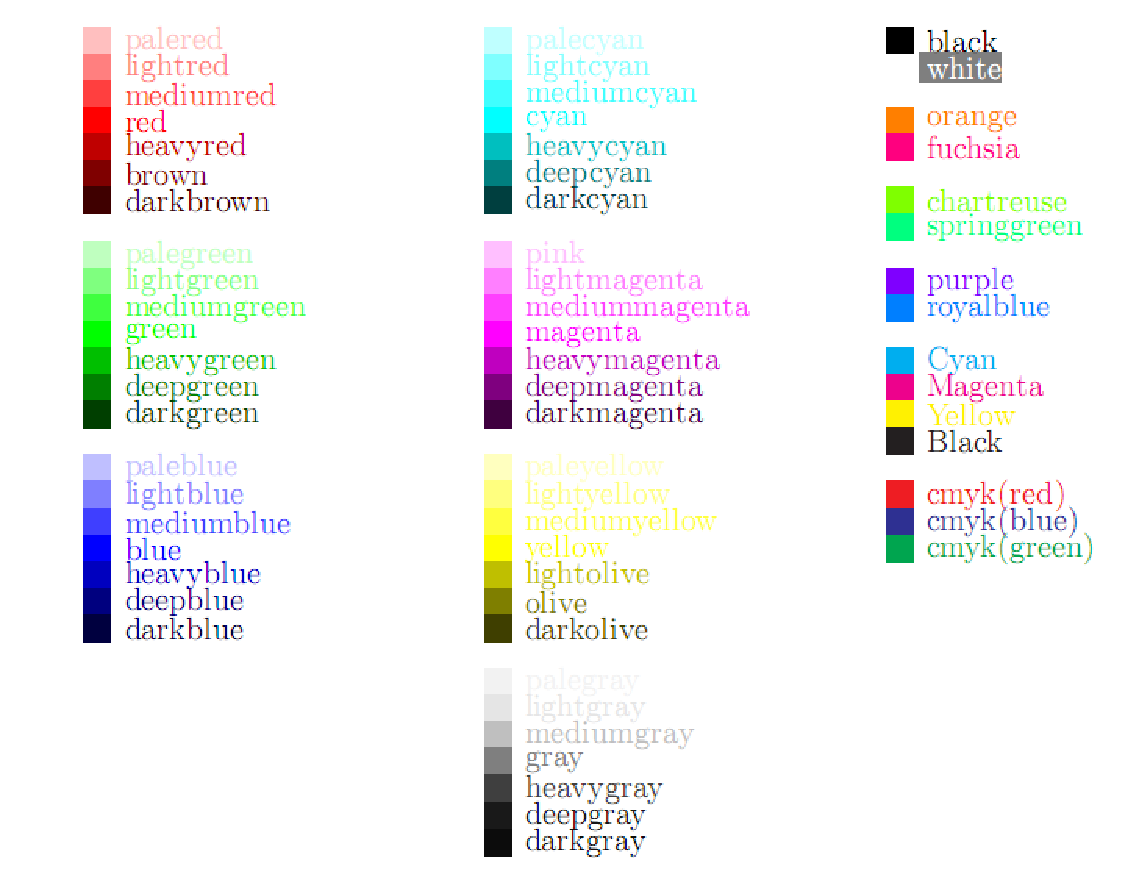
\includegraphics[width=12cm]{colors_name}\\
\caption{asy 各种颜色名称} \label{colors_name}
\end{figure}
  \item[字体:] 默认的字体大小为 12 pt,可以用 defaultpen(pen) 改变。\\
  \fcolorbox{white}{lightgreen}{pen fontsize(real size, real lineskip=1.2*size)}
  \item[线宽:] 默认为 soild 实线类型,0.5dp
  \item[透明度:] opacity 从 0(透明)到 1(不透明)之间先值。
\end{description}
画笔的设置可用如下语句:\\
\fcolorbox{white}{lightgreen}{\parbox{12cm}{
defaultpen(linewidth(0.8)+fontsize(4)+red+opacity(0.5));\\
//设置默认画笔类型\\
pen graypen=linewidth(0.2bp)+gray(0.5);\\
//增加画笔类型
  }}
\clearpage


%%%%%%%%% 点的绘制 %%%%%%%%%%%%%%%%%%%%
\subsection{点的绘制}
%
\subsubsection{空心点,实心点}
dot(参数)表示画实心点;
dot(参数,UnFill)表示画空心点;
参数一般为 pair 二元组的数据类型,表示平面坐标。\\

\lstinputlisting{body/asycode/dots.asy}

\subsubsection{网络格点}
1.自己绘制

\begin{lstlisting}
//`背景网格`
for (int i = 0; i <= 8; ++i) {
  real x = i * cm;
  //`横线`
  draw((0,x)--(8cm,x));
  //`竖线`
  draw((x,0)--(x,8cm));
}
\end{lstlisting}

2.调用 math 模块的 grid 函数\\
\begin{lstlisting}
import math;
add(grid(10,10,gray));
\end{lstlisting}
grid函数使用方法:\\
\begin{lstlisting}
 picture grid(int Nx, int Ny, pen p=currentpen)
\end{lstlisting}


以上为绘制一个 Nx X Ny ,间距为 1 的图形,为 pic 格式。\\
\begin{lstlisting}
add(grid(10,10,gray));
\end{lstlisting}

要使用 grid 函数画的图形,要使用 add(图) 命令,把这个图形加在当前的图上:



\subsubsection{比例分点,中点}
可用这种形式:\textcolor[rgb]{0.00,0.50,0.00}{interp(A,B,t)}
来表示比例分点,其中 t 为比例因子为 real 类型;A,B 为点坐档,pair类型。\\
用 midpoint 函数它们的中点。调用格式是:\textcolor[rgb]{1.00,0.00,0.00}{midpoint(path)},代码如下所示:\\
\begin{lstlisting}
pair X=interp(A,B,t);
pair D=midpoint(A- -B)
\end{lstlisting}


\subsubsection{交点}
调用函数 extension:\\
\begin{lstlisting}
 pair extension(pair P, pair Q, pair p, pair q);
\end{lstlisting}
%
返回线段P\,-\,-\,Q与p\,-\,-\,q延长线的交点,否则,如果两直线平行,返回(infinity,infinity)。

\clearpage

%
%%%%%%%%% 线的绘制 %%%%%%%%%%%%%%%%%%%%
%\subsection{线的绘制}
%
%\subsubsection{实线,虚线}
%代码如下:\\
%
%  \lstinputlisting{body/asycode/lines.asy}
%
%  \begin{description}
%    \item[solid] 可以省略, 表示画实线;
%    \item[dashed ]  画虚线
%    \item[dashdotted] 画点划线
%    \item[dotted ]  画实心点线
%  \end{description}

%\subsubsection{箭头线}
%代码如下:\\
%
%  \lstinputlisting{body/asycode/arrows.asy}
%
%
% \begin{description}
%    \item[Arrow,EndArrow] 效果一样, 都是在路径的末端添加箭头;
%    \item[BeginArrow] 在路径的开头加箭头
%    \item[Arrows] 在路径的头尾都加上箭头
%    \item[MidArrow]  在路径的中间添加箭头
%  \end{description}
%
%\subsubsection{曲线,函数曲线}
%调用 graph 函数,返回类型为 path(guide) 的路径,调用代码格式为:\\
%\begin{center}
%\fcolorbox{white}{lightgreen}{\parbox{12cm}{
%real f(real x)\{return y=x\^{}2;\};\\
%//real x 声明函数自变量 x 是实数型,\\
%//f 前面的 real 声明函数 f 也是一个实数型.\\
%guide graph(real f(real), real a, real b,interpolate join=operator - -);\\
%//描述函数曲线
%  }}
%\end{center}
%
%
%其中:\begin{description}
%        \item[曲线的函数] real f(real x){return y=x}
%        \item[变量范围] a,b
%        \item[画笔线型] 折线:operator - - ;曲线:operator ..
%      \end{description}
%
%  \lstinputlisting{body/asycode/graph_line.asy}\\
%
%\clearpage


%%%%%%%%% 标注 %%%%%%%%%%%%%%%%%%%%
\subsection{标注}
\subsubsection{string 类型}
可包括各种符号,用双引号 " 或单引号 ' 包括起来。空格和换行都会保持不变。
当遇到引号或其他特殊符号时,用\ref{markcode}所示格式进行转义变换。
\begin{table}[htb]
\rowcolors{1}{white}{whiteblue}
\centering
 \caption{ string 类型对应的特殊字符}\label{markcode}
 \begin{tabular}{cc|cc}
  \toprule
    \textbf{换码序列} & \textbf{对应的字符} & \textbf{换码序列} &
    \textbf{对应的字符}\\\midrule
    \verb|\'| & 单引号~\verb|'| & \verb|\"| & 双引号~\verb|"| \\
    \verb|\?| & \verb|?| & \verb|\\| & \verb|\| \\
    \verb|\a| & 报警 & \verb|b| & 退格 \\
    \verb|\f| & 进纸 & \verb|\n| & 换行 \\
    \verb|\r| & 回车 & \verb|\t| & 水平制表符 \\
    \verb|\v| & 竖直制表符 & & \\
    \verb|\0|--\verb|\377| & 八进制编码相应的字符 &
    \verb|\x0|--\verb|\xFF| & 十六进制编码相应的字符 \\
  \bottomrule
 \end{tabular}

\end{table}

\subsubsection{点上的标注}
调用代码如下:

\begin{asycmd}
label(Label,position,align);\\
label("字符串", 点);\\
label("字符串", 点, 方向);\\
Label("字符串",字符旋转方向);\\
label(Label("字符串",字符旋转方向),点,相对点方向);
\end{asycmd}
label 的相对点方向方向有东南西北左中右\textcolor[rgb]{0.00,0.50,0.25}{ LeftSide,RightSide,Center 和 Relative(E或(S,N,W))}\\
Label 的字符旋转方向有东南西北任意角度 \textcolor[rgb]{0.00,0.50,0.25}{Rotate(E或(S,N,W))或 Rotate(x,y)}\\

  \lstinputlisting{body/asycode/label.asy}

\begin{figure}[htbp]
  % Requires \usepackage{graphicx}
  \centering
  
\includegraphics[width=14cm]{body/asycode/label}\\
  \caption{标注方向}\label{label}
\end{figure}


\subsubsection{坐标轴标注}

\begin{lstlisting}
xaxis("$x$",Arrow); //`X 轴下方`
yaxis("$y$",Arrow);//`Y 轴左方` 
\end{lstlisting}



\subsubsection{箭头标注}
\color{red}
\verb|arrow("$t=\frac{1}{3}$",Z,SE);|
\normalcolor

Z 为 pair 类型的点,SE 为相对方向,引号内为标注文字

\subsubsection{中文标注}

在含有中文字符时,前面须加上以下命令:
\begin{lstlisting}
texpreamble("\usepackage{CJK}
 \AtBeginDocument{\begin{CJK*}{GBK}{kai}
   \AtEndDocument{\clearpage\end{CJK*}}");}
\end{lstlisting}

\clearpage


%%%%%%%%% 图形面的绘制 %%%%%%%%%%%%%%%%%%%%
\subsection{面图形的绘制}

\subsubsection{单位圆,单位矩形}
Asymptote 预先定义了很多画基本图形的函数,经常调用的有:\\
\begin{description}
  \item[box] (矩形的左下角, 矩形的右上角);
  \item[ellipse] (椭圆的中心, 水平方向的轴长, 竖直方向的轴长);
  \item[drawline] (直线的第一个点, 直线上的第二个点);
  \item[unitcircle,unitcircle3] 单位圆
  \item[unitsquare,unitsquare3] 单位正方形
  \item[unitsphere] 单位球 - - 3D
  \item[unitbox,unitcube] 正方体 - - 3D
  \item[旋转体函数] 如unitsphere, unitcone, unitcylinder, unitsolidcone,%
  unithemisphere, unitfrustum(real t1, real t2) 等等。
  \item[polygon(n)] 正多边形

\end{description}

  \lstinputlisting{body/asycode/surface.asy}


\begin{figure}[htbp]
  % Requires \usepackage{graphicx}
  \centering
  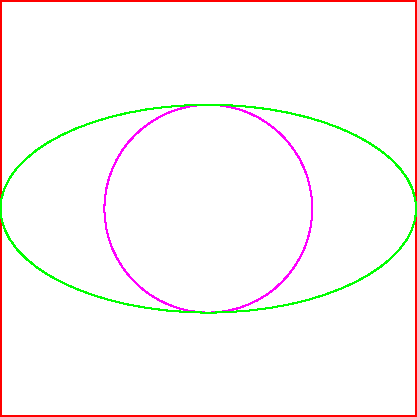
\includegraphics[width=8cm]{body/asycode/surface.pdf}\\
  \caption{对应曲线}\label{surface}
\end{figure}

\subsubsection{封闭曲面}
\clearpage


%%%%%%%%% 图形变换 %%%%%%%%%%%%%%%%%%%%
\subsection{图形变换}
shift,scale,rotate,fill,clip,
\subsubsection{平移,放缩,旋转}
\begin{description}
  \item[平移] shift(x,y)$*$图像
  \item[放缩] xscale(放大倍数)$*$图像: xscale(real x),yscale(real y),scale(real s),scale(real x,real y)
  \item[旋转] rotate(旋转角度, 点坐标),绕点逆时针旋转
  \item[反射] reflect(点a,点b):以 a - - b 为对称轴反射
\end{description}

\subsubsection{填充,裁剪}
\begin{itemize}
  \item add(图像,原点)
  \item add(图像,above=false)
  \item fill(封闭区域,颜色)
  \item filldraw(封闭区域,fillpen=填充颜色,drawpen=路径颜色)
  \item clip(裁剪对象(pic),裁剪路径):裁剪命令处理完后 pic 只剩下裁剪出的部分,可用 add 函数再次加入。
\end{itemize}
\textcolor[rgb]{1.00,0.00,0.50}{picture 类型是一个独立的图,用 draw,filldraw 绘制后不会显示,要显示必须用 add 命令。}


\textcolor[rgb]{0.25,0.50,0.50}{填充阴影}使用 pattern 宏包\\

\begin{minipage}{12cm}
\lstinputlisting{body/asycode/pattern.asy}
\end{minipage}


hatch(NW) 是一种西北走向的阴影斜线的图形; 用\verb$ add("name",hatch(NW))$; 命名为 name。
接下去用 \verb$pattern("name")$ 的方式把它做成一个类似与颜色的画笔。
hatch() 函数还有其他参数, 比如线的粗细, 线的间隔等.



\clearpage


%%%%%%%%% 导入数据 %%%%%%%%%%%%%%%%%%%%
\subsection{导入外部文件}


\subsubsection{导入自定义宏包}
自己做好一些图形后可以将他们保存为模板,方便以后调用,可以将其做成宏包形式,以方便在以后的绘图中导入。

可以将自定义宏包放在和 .asy 代码文件同一文件夹下,或 Asymptote 的安装路径下 \verb$C:\Program Files\Asymptote$

\subsubsection{导入外部数据} 


\subsubsection{导入外部图片} 


%%%%%%%%%%%%%%%% 绘图命令 %%%%%%%%%%%%%%%%%%%%%%
\section{一些图形模板}

\subsection{流程图}
流程图如\ref{do_asy}:
\begin{figure}[H]%位置选项
\centering
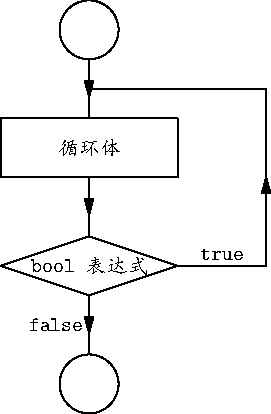
\includegraphics[width=6cm]{do}
\caption{流程图} \label{do_asy}
\end{figure}

代码如下所示:

  \lstinputlisting{figures/do.asy}






\subsection{状态机}
首先将 simplenode.asy 放至 Asymptote 的安装文件夹,再执行 automata 的 asy 文件。
\begin{figure}[H]%位置选项
\centering
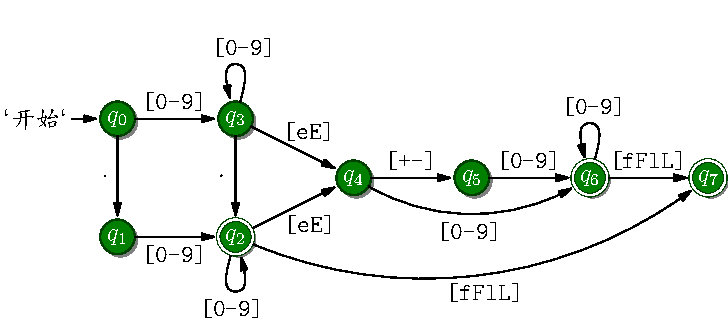
\includegraphics[width=14cm]{body/asycode/automata}
\caption{状态机} \label{automata}
\end{figure}

\subsubsection{源代码}


代码如下所示。\label{code_automata}
  \lstinputlisting{body/asycode/automata.asy}

\subsection{时序图}
\begin{figure}[H]%位置选项
\centering
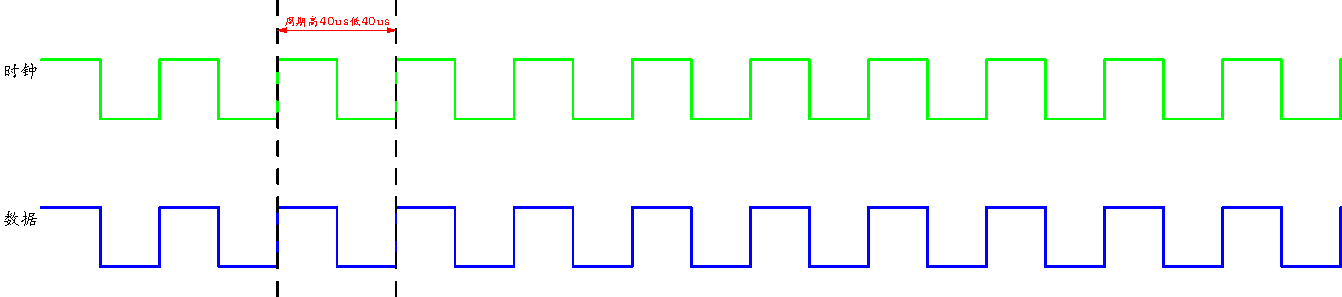
\includegraphics[width=14cm]{body/asycode/wave}
\caption{时序图} \label{wave}
\end{figure}
代码如下所示
\tiny
  \lstinputlisting{body/asycode/wave.asy}
  \normalsize 
       %ASY绘图设计
\clearpage
\bookmarksetup{bold,color=grass}
\chapter{幻灯片制作}
\bookmarksetup{bold=false,color={}}
\thispagestyle{fancy}

~\\[9cm]
\begin{flushright}
\kai\xiaosi
\textcolor[rgb]{0.00,0.50,0.00}{
学不博无以通其变,\\
思不精无以酌其微。\\\footnote{\textcolor[rgb]{0.00,0.50,0.00}{从星际译王作者胡正网页上看到的,感觉很有道理。此人还曾发现 linux 内核的好几处 bug,后看破红尘,研究佛法去了}}\\
}
\end{flushright}



%\section{BEAMER  模板}
\section{BEAMER 模板}
\lstset{language={[LaTeX]TeX}}

\subsection{目录显示}
\index{命令!\verb$\tableofcontents$}

命令为:\\
\fbox{$\backslash$tableofcontents[用逗号分隔的选项]}

其中的主要选项有:\\

\begin{table}[htbp]
  \centering
  \caption{BEAMER 目录可选项}\label{contents}
\begin{tabularx}{14cm}{rX}
\toprule
  currentsection(或 currentsubsection) & 仅正常显示当前节(小节)目录,其他部分半透明 \\
  hideallsubsections & 不显示所有小节目录 \\
  hideothersubsections & 不显示当前节以外所有小节目录 \\
pausesections& 目录逐节显示,相当于每节目录后加上 $\backslash$pause 命令 \\
\bottomrule
\end{tabularx}
\end{table}

\subsection{创建帧}
\index{命令!\verb$\frame$}

\subsubsection{创建与结束}
\begin{lstlisting}[language={[LaTeX]TeX}]
\begin{frame}
\frametitle{...}
...
\end{frame}
`或`
\frame{...}
\end{lstlisting}

\subsubsection{颜色设置}
\index{命令!\verb$\beamersetaveragebackground$}

\begin{lstlisting}[language={[LaTeX]TeX}]
\beamersetaveragebackground{`颜色`}
\end{lstlisting}
用于设置帧背景的颜色\\
\verb$\alert{}$:将字体改为红色,强调用\\
\subsubsection{主题设置}

\index{命令!\verb$\useoutertheme$}
\index{命令!\verb$\useinnertheme$}
\index{命令!\verb$\usecolortheme$}
\index{命令!\verb$\usefonttheme$}
\index{命令!\verb$\usetheme$}


一共有五类主题,外部、内部、颜色、字体、演示。
\begin{lstlisting}[language={[LaTeX]TeX}]
\useoutertheme[`参数`]{`主题名`}
\useinnertheme[`参数`]{`主题名`}
\usecolortheme[`参数`]{`主题名`}
\usefonttheme[`参数`]{`主题名`}
\usetheme[`参数`]{`主题名`}
\end{lstlisting}

\begin{description}
  \item[外部主题] 设定上下边,导航条以及过渡样式

%%%%%%%%%%%%%%%%% 内部主题 %%%%%%%%%%%%%%%%%%%%%%%%%%%%%%%%
  \item[内部主题] 设定内部文本的常规列表(itemize)和排序列表(enumerate)格式及形状
  \begin{enumerate}
    \item default: 标记为小三角
    \item circles: (itemize)的标记改为小圆盘,(enumerate)添加背景圆盘,目录前加小圆盘
    \item rectangles: 跟上面一样,把标记变成方块
    \item rounded:同上,把标记变成圆球,模块背景框直角变圆弧,可选参数[shadow],可给 block 添加阴影。
  \end{enumerate}
%%%%%%%%%%%%%%%%%%%%%%%%%%%%%%%%%%%%%%%%%%%%%%%%%%%%%%%%%%%%%%%

  \item[颜色主题] 设定幻灯片颜色布局
  \item[字体主题] 设定标题,公式,文本,导航条的字体属性

%%%%%%%%%%%%%%%%% 演示主题 %%%%%%%%%%%%%%%%%%%%%%%%%%%%%%%
  \item[演示主题] 以上四种主题的组合排列主题名有下列 5 类:
\begin{enumerate}
  \item 无导航条:default
  \item 侧导航条:从上到下为题名简称,作者姓名,节标题和小节标题

  \begin{tabular}{ll}
    % after \\: \hline or \cline{col1-col2} \cline{col3-col4} ...
    Berkeley: & 左侧+符号条,蓝底白字 \\
    Goettingen: & 右侧+符号条,浅蓝底黑字 \\
    Hannover: & 左侧+符号条,浅蓝底黑字 \\
    Marburg: &  右侧+符号条,深蓝底白字\\
    PaloAlto: & 左侧+符号条,蓝底白字 \\
  \end{tabular}

  \item 顶边导航条
  \item 底边导航条
  \item 顶边+底边导航条
  \begin{itemize}
    \item AnnArbor: 顶边左段青底红字:节标题;右段黄底黑字,小节标题。
    底左蓝底红字,姓名院校;中黄底青字:题名简称;右日期帧码:黄底黑字。
    \item CambridgeUS: 同上,不同的是顶左褐底白字,右为灰底褐字。底左褐底白字,中灰底褐字,右灰底褐字
    \item Copenhagen:同上,底部只分两段,去除了日期和帧码,顶左黑底白字,右为蓝底白字。底左黑底白字,右蓝底白字
    \item Warsaw: 同 Copenhagen,在 block 外加了阴影,增加立体感
  \end{itemize}
\end{enumerate}
%%%%%%%%%%%%%%%%%%%%%%%%%%%%%%%%%%%%%%%%%%%%%%%%%%%%%%%%%%%%%%%

\end{description}


\subsubsection{加入时钟}

\index{命令!\verb$\initclock$}
\index{宏包!tdclock}

使用 tdclock 时钟宏包,\verb$\initclock$的时钟命令,如下所示
\begin{lstlisting}[language={[LaTeX]TeX}]
\usepackage[timeinterval=1]{tdclock}
\date[\initclock\tdtime]{\today}
\end{lstlisting}

\subsection{block 文本模块}
block 模块可以创建一个矩形区域,分标题和文本两块,用不同的颜色加以区别
\subsubsection{定理类}

包括定义、定理、证明、示例等环境(theorem、 definition、 lemma、 proof、 corollary、 problem)
显示的是带标题和文本两框的形式。用以下代码中文化,和引用。
\begin{lstlisting}[language={[LaTeX]TeX}]
\setbeamertemplate{theorems}[numbered]
`在定理后加数字,默认不加`
\begin{document}
\newtheorem{THeorem}{`定理`}
\newtheorem{DEfinition}{`定义`}
\newtheorem{PRoof}{`证明`}
\begin{theorem}
`文本框文字`
\end{theorem}
\begin{THeorem}
`文本框文字`
\end{THeorem}
\end{document}
\end{lstlisting}

\subsubsection{文本框}

\index{命令!\verb$\begin{block}$}
\index{命令!\verb$\begin{exampleblock}$}
\index{命令!\verb$\begin{alertblock}$}

有 block、exampleblock 和 alertblock 三种,用法如下:\\
\begin{lstlisting}[language={[LaTeX]TeX}]
\begin{block}{`标题栏文字`}
`文本框文字`
\end{block}
\end{lstlisting}

\subsubsection{文本盒子}

\index{beamer 环境!\verb$beamercolorbox$}
\index{beamer 环境!\verb$beamerboxesrounded$}

修饰文本的盒子环境,有彩色盒子环境 beamercolorbox 和圆角盒子环境 beamerboxesrounded 两种。
\begin{itemize}
  \item 彩色盒子:单独区域

\color{grass}
\begin{minipage}{12cm}
\verb$\begin{beamercolorbox}[参数]{beamer颜色}$\\
内容\\
\verb$\end{beamercolorbox}$
\end{minipage}
\normalcolor

其中参数的设置有:

\begin{tabular}{ll}
  wd=宽度 & 盒子宽度,默认为\verb$\textwidth$,文本行宽度 \\
  rounded=true & 盒子改为圆角 \\
  shadow=true & 增加阴影,当 rounded=true 时才有效 \\
  colsep=宽度 & 文本与盒子四边的距离 \\
  colsep$*$= & 文本与盒子上下边的距离 \\
  center & 文本与盒子水平居中对齐,默认为左对齐 \\
\end{tabular}

  \item 圆角盒子:包括标题区域和文本区域


\color{grass}
\begin{minipage}{12cm}
\verb$\begin{beamerboxesrounded}[参数]{标题}$\\
内容\\
\verb$\end{beamerboxesrounded}$
\end{minipage}
\normalcolor

\begin{tabular}{ll}
   width=宽度 & 盒子宽度 \\
  shadow=true & 增加阴影,当 rounded=true 时才有效 \\
  upper=beamer 颜色 & 标题区域的前景色与背景色 \\
  lower=beamer 颜色 & 文本区域的前景色与背景色 \\
\end{tabular}
\end{itemize}

\subsubsection{列表}

\index{beamer 命令!\verb$\setbeamercovered$}

主要两个命令进行控制逐幅显示
\begin{lstlisting}[language={[LaTeX]TeX}]
\setbeamercovered{transparent}%`逐幅显示的内容为半透明`
\begin{enumerate}
  \item `文本1`
  \pause
  \item `文本2`
\end{enumerate}
\end{lstlisting}


\subsection{分栏显示}
\subsubsection{minipage 环境实现多栏}
\index{环境!minipage}

可将幻灯片分为多栏,通常为 2 栏,如下所示:
\begin{lstlisting}[language={[LaTeX]TeX}]
\begin{minipage}[]{`宽度`}
\end{minipage}
\begin{minipage}[]{`宽度`}
\end{minipage}
\end{lstlisting}

对齐参数有:\\
\begin{tabular}{ll}

  b & 底行对齐 \\
  c & 中心对齐 \\
  t & 第一行对齐(基线) \\
  T & 第一行对齐(顶部) \\

\end{tabular}
\subsubsection{columns 环境实现多栏}
\index{beamer 命令!\verb$\column$}
可根据内部的 column 环境自动分栏。如下所示:
\begin{lstlisting}
\begin{columns}
\begin{column}[t]{5cm}
Two\\lines.
\end{column}
\begin{column}[t]{5cm}
Oneline(butaligned).
\end{column}
\end{columns}
% 或者
\begin{columns}
\column[t]{5cm}
Two\\lines.
\column[t]{5cm}
One line(but aligned).
\end{columns}
\end{lstlisting}

可选择项内参数有
\begin{itemize}
  \item b:底部对齐
  \item c:中心对齐
  \item t:顶部基线对齐
  \item T:顶部对齐
  \item onlytextwidth:相当于 totalwidth=\verb|\textwidth|
  \item totalwidth=\verb|{width}| :columns 默认是整幅帧宽度,可自定义宽度
\end{itemize}

\subsection{导航板设置}

\subsubsection{sidebar 参数设置}
\index{beamer 命令!\verb$\useoutertheme$}
共6个可选参数
\scriptsize
\begin{lstlisting}[language={[LaTeX]TeX}]
\useoutertheme[height=0.1\textwidth,width=0.15\textwidth,hideothersubsections,right]{sidebar} \end{lstlisting}
\normalsize
\begin{description}
  \item[height] 标题的高度
  \item[hideothersubsections]  显示所有的 subsection
  \item[hideallsubsections] 不显示subsections
  \item[left] 放在左边
  \item[right] 放在右边
  \item[width] sidebar 导航栏的宽度
\end{description}

\subsubsection{对应的目录导航有颜色显示}
\index{beamer 命令!\verb$\usecolortheme$}
使用如下主题
\begin{lstlisting}[language={[LaTeX]TeX}]
\usecolortheme{sidebartab}
\end{lstlisting}
\subsubsection{导航板logo设置}
\index{beamer 命令!\verb$\logo$}
\begin{lstlisting}[language={[LaTeX]TeX}]
\logo{\includegraphics[height=0.09\textwidth]{wuda.pdf}}
\end{lstlisting}

\subsection{时间设置}

\index{命令!\verb$\initclock$}
\index{宏包!tdclock}



下载 tdclock 宏包,用法如下:
\begin{lstlisting}[language={[LaTeX]TeX}]
\usepackage[`参数`]{tdclock}
\usepackage[timeduration=60,timewarningfirst=90,
timewarningsecond=95,colorwarningfirst=blue,
fillcolorwarningfirst=white!60!yellow,
fillcolorwarningsecond=white!10!yellow,timedeath=1]{tdclock}
\end{lstlisting}
\begin{tabular}{ll}
  timeinterval=n & n 秒更新一次 \\
  timeduration=n & n 分钟完成时间 \\
  timewarningfirst=n & 剩 n 秒后颜色变化默认90 (1-100)\\
  timewarningsecond=n & 剩 n 秒后颜色变化默认95 (1-100)\\
  colorwarningsecond=color  & 字体颜色 \\
  fillcolorwarningsecond=color & 背景颜色 \\
  timedeath=0or1 & 1为超过 110\%时间后关闭,0不关闭 \\
\end{tabular}



在之前须有\verb|\initclock|来进行时钟初始化,引用时间代码如下所示:\\
\begin{table}[ht]
\caption{引用时间对应代码} \centering
\rowcolors{2}{lightblue}{whiteblue}
\begin{tabular}{clcl}
\toprule
 % after \\: \hline or \cline{col1-col2} \cline{col3-col4} ...
时钟代码 & 对应时间 & 秒表代码 & 对应显示时间\\
  \verb|\tdclock| & 日期+时间 & \verb|\crono| & 时:分:秒 \\
  \verb|\tdtime| & 时间 & \verb|\cronohours| & 时 \\
  \verb|\tddate| & 日期 & \verb|\cronominutes| & 分 \\
  \verb|\tdday| & 日 &  \verb|\cronoseconds| & 秒  \\
  \verb|\tdmonth| & 月 & \verb|\resetcrono{"button"}| & 复位秒表 \\
  \verb|\tdyear| & 年 & \verb|\toggleclock{"button"}|& 秒表、时钟切换\\
  \verb|\tdhours| & 时 && \\
  \verb|\tdminutes| & 分 && \\
  \verb|\tdseconds| & 秒 && \\
  \bottomrule
\end{tabular}
\end{table}
~\\
PDF 样例\\
\begin{center}
\textattachfile{tdclock.pdf}{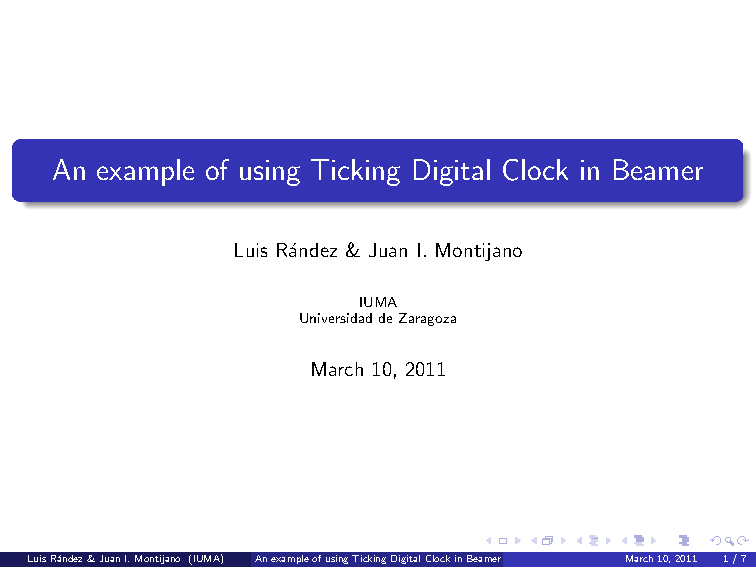
\includegraphics[width=10cm]{body/tdclock_face.pdf}}\\
\end{center}

\subsection{加入附件}

\index{命令!\verb$\textattachfile$}
\index{命令!\verb$\attachfile$}
\index{命令!\verb$\notextattachfile$}
\index{命令!\verb$\noattachfile$}

使用 attachfile2 宏包,可加入真 3d pdf,MS 的 word,excel等,可双击直接打开。
但压缩文件 rar 类型不能从附件中下载,可将 RAR 的压缩文件后缀改成 ar ,
从 pdf 的附件下载后再将后缀改为 rar 类型即可。

引用代码:
\begin{lstlisting}[language={[LaTeX]TeX}]
\usepackage{attachfile2}
`四种引用方式`
\textattachfile{`附件名称`}{`显示图片或文字`}
\attachfile[icon=`图标名称`]{`附件名称`}
`以下两种只显示名称,不加入附件`
\notextattachfile{`附件名称`}{`显示图片或文字`}
\noattachfile[icon=`图标名称`]{`附件名称`}
\end{lstlisting}

icon= 有四种参数,如下图所示:

\begin{figure}[htbp]%位置选项
\centering
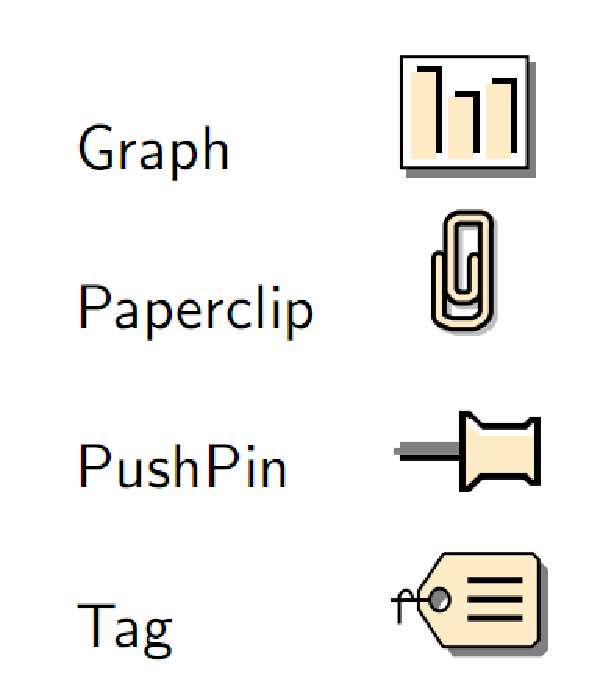
\includegraphics[width=4cm]{icon.pdf}
\caption{附件显示图标} \label{icon}
\end{figure}


\subsection{遮盖,逐步显示}

\subsubsection{遮盖命令}
\index{命令!\verb$\pause$}
\index{命令!\verb$\uncover$}
\index{命令!\verb$\only$}
\index{命令!\verb$\alt$}
\index{命令!\verb$\visible$}
用以下命令可以实现遮盖的效果。
\begin{itemize}
  \item \verb|\pause|:
  \item \verb|\uncover|:
  \item \verb|\only<n->|:只在第 n 张中显示
  \item \verb|\alt|:变换命令
\end{itemize}
对应命令 \verb|\only,\alt,\visible,\uncover,\invisible|有相应的环境 onlyenv, altenv, visibleenv, uncoverenv, invisibleenv,在环境中的元素相当于加入了命令。

\index{环境!overylayarea}
在前后两张 slide 中的同一位置实现内容的改变可用 overlayarea 环境。这样后一张 slide 的内容出现位置会在前一张设定的区域内
\begin{cmd}
\begin{overlayarea}{area width}{area height}
environment contents
\end{overlayarea}
 example:
\begin{frame}
\begin{overlayarea}{\textwidth}{3cm}
\only<1>{Some text for the first slide.\\Possibly several lines long.}
\only<2>{Replacement on the second slide.}
\end{overlayarea}
\end{frame}
\end{cmd}

\subsubsection{表格逐列显示}

\index{命令!\verb$\onslide<n->stuff$}

\verb|\onslide<n->stuff|命令,代码如下表所示:
\begin{shaded}
\begin{Verbatim}
\begin{tabular}{l!{\vrule}c<{\onslide<2->}c<{\onslide<3->}%
c<{\onslide<4->}c<{\onslide}c}
Class & A & B & C & D\\
X & 1 & 2 & 3 & 4\\
Y & 3 & 4 & 5 & 6\\
Z & 5 & 6 & 7 & 8
\end{tabular}
\end{Verbatim}
\end{shaded}
\subsubsection{列表逐项显示}

\index{命令!\verb$\item<n->$}
\index{命令!\verb$\item<+->$}

\begin{shaded}
\begin{Verbatim}
\item<n->  : n 表示从第 n 张开始显示
<+->    : 自动逐项显示
\item<n1-n2>    : 手动控制显示顺序
\end{Verbatim}
\end{shaded}

效果如下,双击显示\footnote{建议用 Adobe Reader 9 以上阅读器}:\\
\begin{enumerate}
  \item  \textcolor[rgb]{1.00,0.00,0.00}{手动控制逐步显示 }\\~\\
\textattachfile{stepview1.pdf}{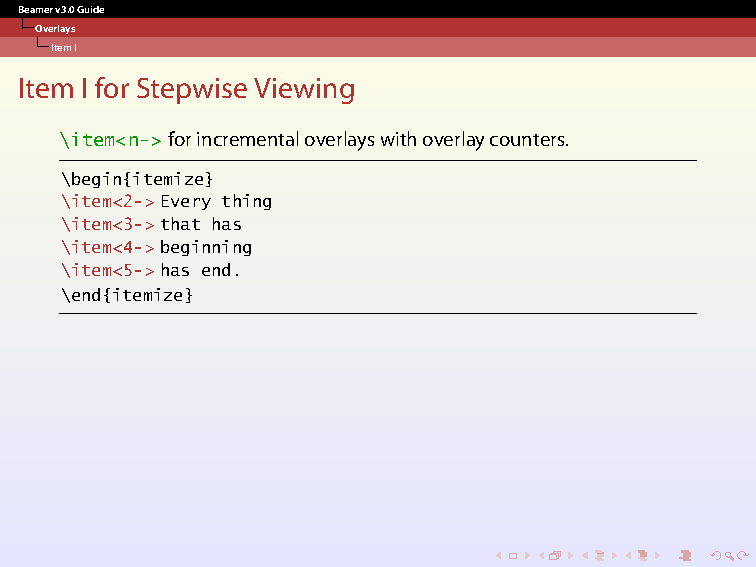
\includegraphics[width=10cm]{body/stepview1_face.pdf}}\\
  \item \textcolor[rgb]{1.00,0.00,0.00}{自动控制逐步显示}\\~\\
\textattachfile{stepview2.pdf}{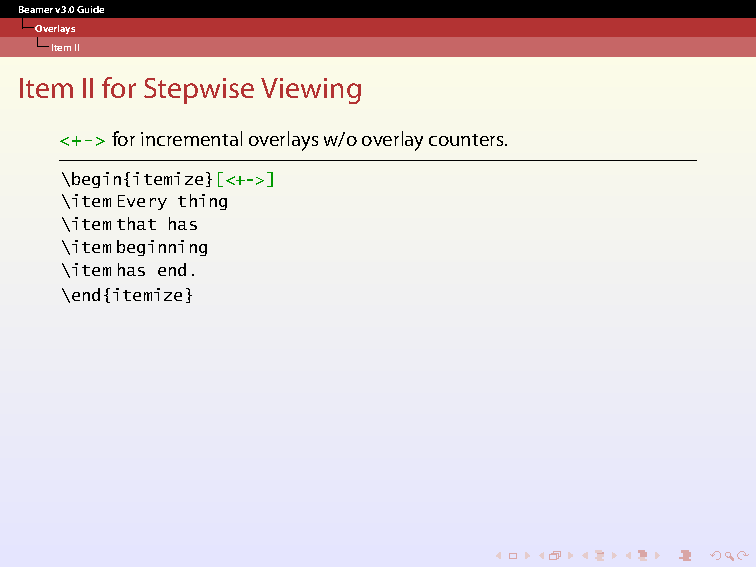
\includegraphics[width=10cm]{body/stepview2_face.pdf}}\\
  \item \textcolor[rgb]{1.00,0.00,0.00}{手动控制跳跃显示}\\~\\
\textattachfile{stepview3.pdf}{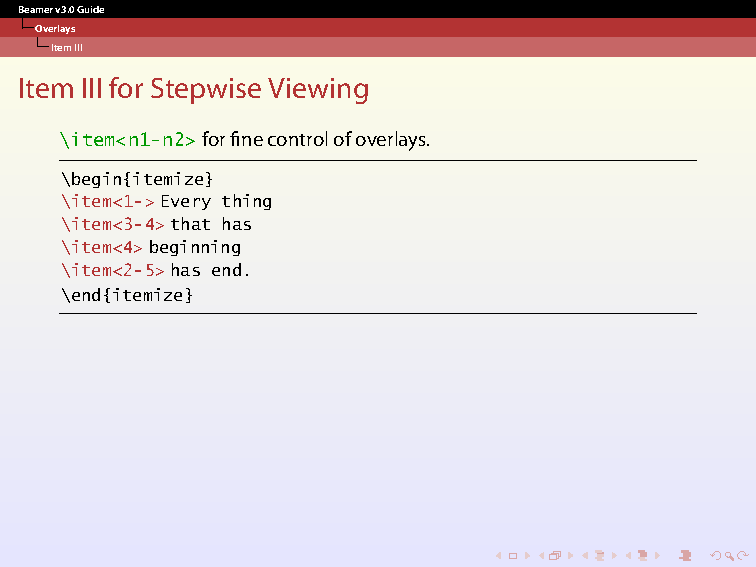
\includegraphics[width=10cm]{body/stepview3_face.pdf}}\\
\end{enumerate}

\subsubsection{内容逐项变化}

\index{命令!\verb$\only<n>$}
\index{命令!\verb$\uncover<n>$}
\index{命令!\verb$\invisible<n>$}
\index{命令!\verb$\alt<n>$}
\index{命令!\verb$\temporal<n>$}

\begin{shaded}
\begin{Verbatim}
\only<n>{..}
在第n张显示括号内的内容,连续性显示。
\uncover<n>{..}
只在第n张显示括号内的内容
\invisible<n>{..}
只在第n张内隐藏括号内的内容
\alt<n>{内容1}{内容2}
在第n张显示内容1,其它张显示内容2
\temporal<n>{内容1}{内容2}{内容3}
第n张前显示内容1,第n张显示内容2,第n张后显示内容3
\end{Verbatim}
\end{shaded}
\textcolor[rgb]{1.00,0.00,0.00}{效果如下所示}\\~\\
\textattachfile{replace1.pdf}{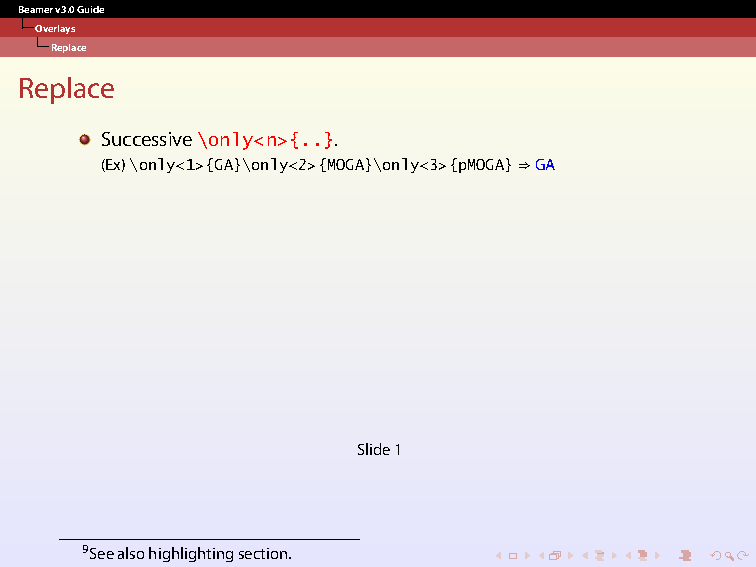
\includegraphics[width=10cm]{body/replace1_face.pdf}}\\
\subsubsection{列表逐项高亮变色}
有四种方案:\\

\index{命令!\verb$\item <+-| alert@+>$}

\begin{enumerate}
  \item \textcolor[rgb]{1.00,0.00,0.00}{从无到有的高亮}\\~\\
\textattachfile{highlight1.pdf}{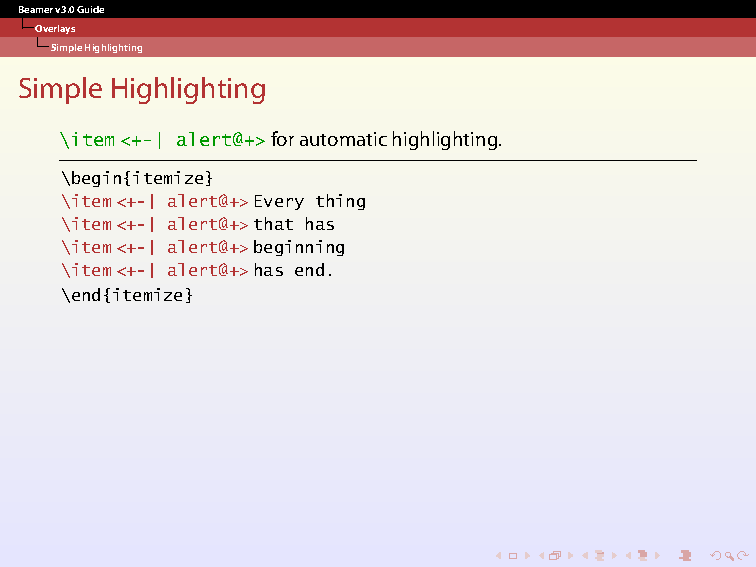
\includegraphics[width=10cm]{body/highlight1_face.pdf}}\\
\begin{shaded}
\begin{Verbatim}
\begin{itemize}[<+-|alert@+>]
以上为自动逐项高亮
\item <+-| alert@+>
以上为手动为每项加高亮
\end{Verbatim}
\end{shaded}


  \item \textcolor[rgb]{1.00,0.00,0.00}{全显示逐步高亮}\\~\\


\index{命令!\verb$\item<2-| alert@2>$}

  \textattachfile{highlight2.pdf}{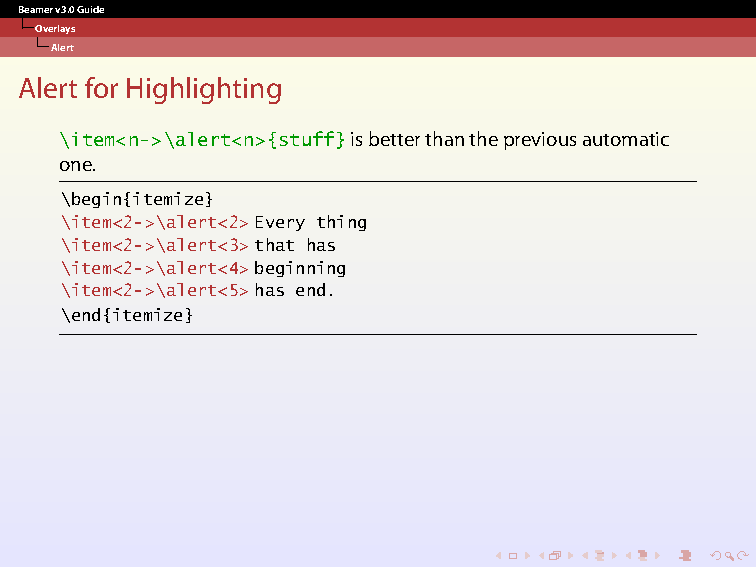
\includegraphics[width=10cm]{body/highlight2_face.pdf}}\\
\begin{shaded}
\begin{Verbatim}
\item<n->\alert<n>{stuff}
第n张显示高亮
\item<2->\alert<2>
\item<2-| alert@2>
以上两种效果相同
\end{Verbatim}
\end{shaded}

  \item \textcolor[rgb]{1.00,0.00,0.00}{可配置底色高亮}\\~\\

\index{命令!\verb$\alt<n>$}

  \textattachfile{highlight3.pdf}{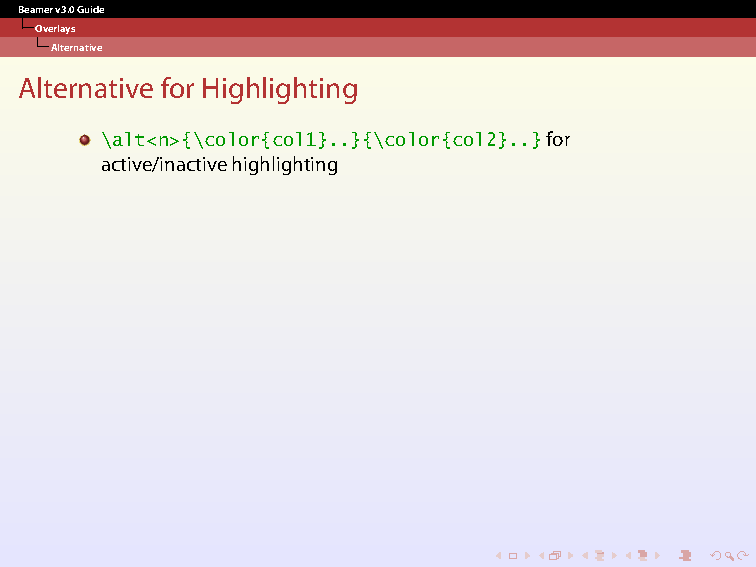
\includegraphics[width=10cm]{body/highlight3_face.pdf}}\\
\begin{shaded}
\begin{Verbatim}
\alt<n>{\color{col1}..}{\color{col2}..}
前面的括号是高亮时的颜色和内容,后面是不高亮时的颜色和内容
\end{Verbatim}
\end{shaded}

  \item \textcolor[rgb]{1.00,0.00,0.00}{高亮后底色变化}\\~\\

\index{命令!\verb$\temporal<n>$}

  \textattachfile{highlight4.pdf}{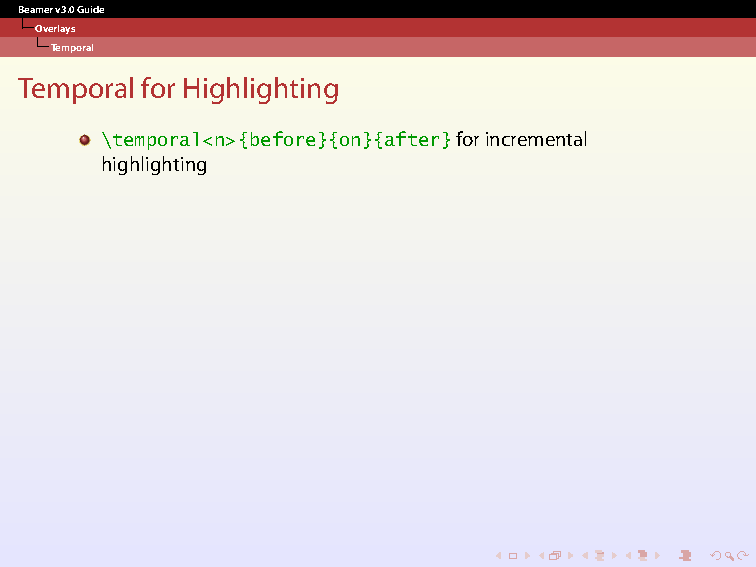
\includegraphics[width=10cm]{body/highlight4_face.pdf}}\\
\begin{shaded}
\begin{Verbatim}
\def\hilite<#1>{%
\temporal<#1>{\color{gray}}{\color{blue}}%
{\color{blue!25}}}
...
\temporal<n>{before}{on}{after}
before 为高亮前颜色,on 为高亮颜色,after 为高亮后颜色。

\end{Verbatim}
\end{shaded}
\end{enumerate}



%%%%%%%%%%%%%%%%%%%%%%%%%%%%%%%%%%%%%%%%%%%%%%%%%%%%%%%%%%%%
\subsection{代码抄录 semiverbatim lstlisting}
可用 verbatim 和 lstlisting 环境,semiverbatim 环境类似于 verbatim ,但里面的 \verb|\,{,}| 符号保持原意,在 semiverbatim 环境中可用 \verb|\\,\{,\}| 来表示原符号。使用以上环境时必须在\verb|\begin{frame}|后加上可选项 fragile。\verb|\begin{frame}[fragile]|。

%%%%%%%%%%%%%%%%%%%%%%%%%%%%%%%%%%%%%%%%%%%%%%%%%%%%%%%%%%%%
\subsection{切换颜色}


beamer 颜色由三类构成:
\begin{itemize}
  \item Navigational bars
  \item Background
  \item Structure
\end{itemize}
\subsubsection{定义新颜色}
\begin{shaded}
\begin{Verbatim}
颜色1!百分比1!颜色2
%颜色2占有剩下的百分比
green!80!gray
%表示80%green加20%gray
-green
%表示从以前的颜色移除green
\end{Verbatim}
\end{shaded}
\subsubsection{改变 alert 颜色}
如\ref{alert change}所示

\begin{figure}[H]
  \centering
  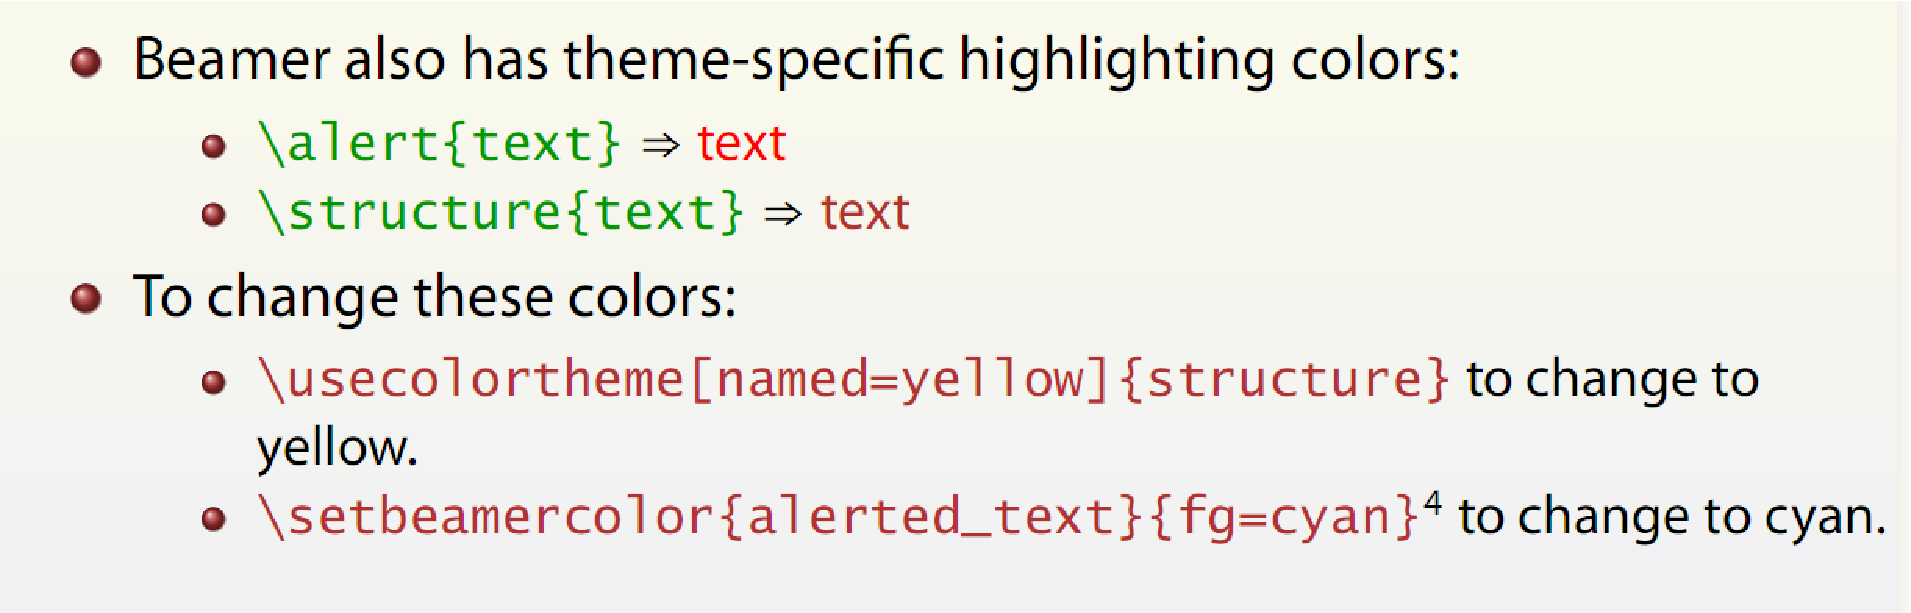
\includegraphics[width=12cm]{coloralertstructure}\\
  \caption{改变 alert 颜色}\label{alert change}
\end{figure}
\subsubsection{改变 background 颜色}

\index{命令!\verb$\beamersetaveragebackground$}
\index{命令!\verb$\beamertemplatesolidbackgroundcolor$}
\index{命令!\verb$\beamertemplateshadingbackground$}
\index{命令!\verb$\beamertemplategridbackground$}

有实体、倾斜、格点三种颜色模式。
\begin{shaded}
\begin{Verbatim}
%soild颜色
\beamersetaveragebackground{color} or
\beamertemplatesolidbackgroundcolor{color}
%gradient颜色
\beamertemplateshadingbackground{color1}{color2}.
% The colors in this slide is {blue!5}{yellow!10}.
%grid颜色
\beamertemplategridbackground[grid_space].
\end{Verbatim}
\end{shaded}
\subsubsection{改变 structure 颜色}


\index{命令!\verb$\colorlet$}
\index{命令!\verb$\usestructuretemplate$}
\index{命令!\verb$\beamertemplateshadingbackground$}

\begin{shaded}
\begin{Verbatim}
\colorlet{mystruct}{structure}%Save current structure
\colorlet{structure}{magenta}%New structure
\usestructuretemplate{\color{structure}}{}%\structure{..}
\beamertemplateshadingbackground{yellow!50}{magenta!50}
%New background
\frame{%
...
}%
%Back to the original "structure" and bgcolor schemes
\colorlet{structure}{mystruct}
\beamertemplateshadingbackground{blue!10}{yellow!10}
\end{Verbatim}
\end{shaded}


\subsection{带进度条的幻灯片}
如下图所示:
\begin{figure}[H]
  % Requires \usepackage{graphicx}
\centering
  
\includegraphics[width=12cm]{nav_beamer}\\
  \caption{带进度条的 BEAMER 幻灯片}\label{nav_beamer}
\end{figure}

需把 beamerouterthemeprogressbar.sty 文件放在同一文件夹下,在 BEAMER 的  tex 文件中加入:
\begin{cmd}
  \useoutertheme{progressbar}
\end{cmd}
注意原网络上下载的宏包有错误,须将其代码进行更正后方能编译成功。附件中为已更正的宏包。原宏包更改方式为:
把宏包中的代码:
\begin{lstlisting}
\draw (\progressbar@leftbar, 0.11cm)
[draw=bg!70!fg, rounded corners=0.1cm]
rectangle ++(\progressbar@barlength mm, 0.2cm);
\end{lstlisting}
替换成下面的代码:
\begin{lstlisting}
\draw (\progressbar@leftbar, 0.11cm)
[draw=bg!70!fg, rounded corners=0.1cm]
rectangle ++(\progressbar@barlength*.1cm, 0.2cm);
\end{lstlisting}
即可。

\subsection{note 添加笔记}

可以用来给 beamer 增加讲义,可将讲义单独输出,或混合输出各种方式。
\begin{cmd}
\note{text} % 使用方式
\setbeameroption{show notes} % include notes and normal text
\setbeameroption{hide notes} % default, hide notes page
\setbeameroption{show only notes} % output only notes page
\setbeameroption{show notes on second screen={location} % left,bottom,top
\end{cmd}





%\section{pdfscreen 模板}
\section{pdfscreen 模板}
使用游道德之平林模板改写
\subsection{模板选项}
导言区读入宏包命令为:\\
\fbox{$\backslash$usepackage[screen,panelleft]{pdfscreen}}

其中的主要选项有:\\
\begin{table}[htbp]
  \centering
  \caption{pdfscreen 模板可选项}\label{panel_pdfscreen}
\begin{tabularx}{14cm}{rX}
\toprule
  screen(或 print) & 屏幕输出(打印输出)版本 \\
  panelleft(或 panelright) & 导航板居左(右) \\
  nopanel & 无导航板 \\
paneltoc & 目录放在面板上,但在正文中有 tableofcontents 命令,本命令失效 \\
sectionbreak & 在每一节前面分页 \\
\bottomrule
\end{tabularx}
\end{table}

\subsection{导言中必需出现的命令}
其中的主要选项有:\\
\begin{table}[htbp]
  \centering
  \caption{pdfscreen 导言中命令}\label{command_pdfscreen}
\begin{tabularx}{14cm}{lX}
\toprule
  $\backslash$screensize\{高度\}\{宽度\} & 屏幕尺寸,必须出现 \\
  $\backslash$margins\{左边\}\{右边\}\{顶部\}\{底部\} & 页边宽度,必须出现 \\
  $\backslash$overlay\{图形文件\} & 选取背景图形 \\
  $\backslash$overlayempty & 无背景图形 \\
  $\backslash$paneloverlay\{图形文件\} & 选取导航板背景图形 \\
  $\backslash$paneloverlayempty & 导航板无背景图形 \\
 $\backslash$changeoverlay & 出现此命令,每一新节自动更改背景图形,从 overlay0.pdf 到 overlay10.pdf ,循环使用\\
 $\backslash$urlid\{URL 地址\} & 导航板‘HOME PAGE’指向的地址\\
\bottomrule
\end{tabularx}
\end{table}

       %幻灯片设计
\clearpage
\bookmarksetup{bold,color=grass}
\chapter{一些问题}
\bookmarksetup{bold=false,color={}}
\thispagestyle{fancy}


~\\[9cm]
\begin{flushright}
\kai\xiaosi
\textcolor[rgb]{0.00,0.50,0.00}{
书不记,熟读可记\\ 义不精,细思可精\\
惟有志不立,直是无著力处\\
- - 朱熹
}
\end{flushright}


%%%%%%%%%%%%%%%%%%%%%%%%%%%%%%%%%%%%%%%%%%%%%%%%%%%%%%%%%%%%%%%%%%%%

%\section{文档问题}

\section{文档问题}
\newcounter{buzhou_latex} %不同环境计数器的名称也必需不同
\begin{list}
{\bfseries\sffamily 问题\,\arabic{buzhou_latex}:\hfill}
{\setlength{\parsep}{\parskip}
 \setlength{\itemsep}{0ex plus0.1ex}
 \setlength{\labelwidth}{4em}
 \setlength{\labelsep}{0.2em}
 \setlength{\leftmargin}{6.2em}
 \setlength{\rightmargin}{2em}
 \usecounter{buzhou_latex} \setcounter{buzhou_latex}{0}
 \upshape
}

%\addcontentsline{toc}{subsection}{\qquad$\bigstar$ 问题列表}

\addcontentsline{toc}{subsection}{$\bullet$~合并图表目录}
\item
\color{red}
图表目录合并\\
\normalcolor

用宏包 tocloft




%%%%%%%%%%%%%%%%%%%%%%%%%%%%%%%%%%%%%%%%%%%%%%%%%%%%%%%%%%%%%%

\addcontentsline{toc}{subsection}{$\bullet$~目录链接不正确}

\item
\color{red}
标签页链接不正确\\
\normalcolor

\begin{lstlisting}[language={[LaTeX]TeX}]
\clearpage
\phantomsection
\tableofcontents

\clearpage
\phantomsection
\listoffigures
\listoftables
\end{lstlisting}

%%%%%%%%%%%%%%%%%%%%%%%%%%%%%%%%%%%%%%%%%%%%%%%%%%%%%%%%%%%%%%

\addcontentsline{toc}{subsection}{$\bullet$~表格内换行}
\item
\color{red}
表格内换行,box 内换行\\
\normalcolor

$\backslash$par 命令或\verb|\makecell|命令(需 makecell 宏包)或
\textcolor[rgb]{0.00,0.00,0.63}{使用$\backslash$parbox[t(bsc)默认是 c]\{长度\}\{可使用换行符\}}\\
t(bsc)默认是 c ,可缺省。



%%%%%%%%%%%%%%%%%%%%%%%%%%%%%%%%%%%%%%%%%%%%%%%%%%%%%%%%%%%%%%

\addcontentsline{toc}{subsection}{$\bullet$~PDF 标签乱码}
\item
\color{red}
PDF 标签乱码\\
\normalcolor

重新点 set main file 的图标,重新编译两次\footnote{仅对《 LATEX 入门与提高 第二版》光盘中附赠的 winedt 软件有效,
其他版本的 winedt 在执行完 2 遍 pdflatex 后,再执行 gbk2uni 不带后缀的文件名,再执行一遍 paflatex。}。



%%%%%%%%%%%%%%%%%%%%%%%%%%%%%%%%%%%%%%%%%%%%%%%%%%%%%%%%%%%%%%
\addcontentsline{toc}{subsection}{$\bullet$~图片一直放在文字后}
\item
\color{red}
图片不放在文字前面\\
\normalcolor

 在宏包里使用 flafter 宏包即可


%%%%%%%%%%%%%%%%%%%%%%%%%%%%%%%%%%%%%%%%%%%%%%%%%%%%%%%%%%%%%%

\addcontentsline{toc}{subsection}{$\bullet$~图片强制就地放置}
\item
\color{red}
图片就地放置\\
\normalcolor


        加载 float 宏包,使用\verb$\begin{figure}[H]$命令,\verb$\begin{figure}[h]$中 h 为建议就地放置,H 为命令就地放置。
        H 只能单独使用,不能和其他参数 htbp 混合,否则失去作用。


%%%%%%%%%%%%%%%%%%%%%%%%%%%%%%%%%%%%%%%%%%%%%%%%%%%%%%%%%%%%%%

\addcontentsline{toc}{subsection}{$\bullet$~latex 公式到 word}
\item
\color{red}
公式复制到 word 中\\
\normalcolor


        可先直接复制到 mathtype6.0 ,自动转换成 word 格式


%%%%%%%%%%%%%%%%%%%%%%%%%%%%%%%%%%%%%%%%%%%%%%%%%%%%%%%%%%%%%%

\addcontentsline{toc}{subsection}{字体颜色不均}
\item
\color{red}
用pdflatex生成的字体粗细不一\\
\normalcolor

 字体支持不太好,改用 \LaTeX + dvitopdf 或改用 XeLaTeX (须改设置,utf-8格式,Xecjk 宏包等),


%%%%%%%%%%%%%%%%%%%%%%%%%%%%%%%%%%%%%%%%%%%%%%%%%%%%%%%%%%%%%%


\addcontentsline{toc}{subsection}{$\bullet$~box 环境内的抄录环境}
\item
\color{red}
box 环境内不用用摘录环境\\
\normalcolor

        用 minipage 环境,verbinput 导入外部文件。


%%%%%%%%%%%%%%%%%%%%%%%%%%%%%%%%%%%%%%%%%%%%%%%%%%%%%%%%%%%%%%

\addcontentsline{toc}{subsection}{$\bullet$~PDF 属性中加入作者和文章信息}

\item
\color{red}
在 pdf 属性中加入作者和标题信息。\\
\normalcolor

        使用 hyperref 宏包,在可选项中加入(放在document文档中可以有中文,若在导言区有中文\XeLaTeX 下可能有问题):\\
        \fcolorbox{white}{lightgreen}{
        \parbox{10cm}{
          pdfauthor=\{\},\%作者\\
          pdfkeywords=\{latex\},\%关键词\\
          pdfsubject=\{late beamer asymptote\},\%主题\\
          pdftitle=\{handbook of latex\},\%标题\\
        }}


%%%%%%%%%%%%%%%%%%%%%%%%%%%%%%%%%%%%%%%%%%%%%%%%%%%%%%%%%%%%%%


\addcontentsline{toc}{subsection}{$\bullet$~总页码计数器}
\item
\color{red}
页码后标上总页码对比\\
\normalcolor

使用 lastpage 宏包,用\verb|\pageref{LastPage}|显示总页码
\textcolor[rgb]{1.00,0.00,0.00}{注意此宏包与 movie15 animate 动画影音宏包有冲突。会导致动画和视频不能正常显示}
\begin{shaded}
\begin{Verbatim}
\usepackage{lastpage}
\pageref{LastPage}
\fancyfoot{\thepage/\pageref{LastPage}}
\end{Verbatim}
\end{shaded}
%%%%%%%%%%%%%%%%%%%%%%%%%%%%%%%%%%%%%%%%%%%%%%%%%%%%%%%%%%%%%%

\addcontentsline{toc}{subsection}{$\bullet$~章节页加页眉}
\item
\color{red}
章节页加页眉\\
\normalcolor


在此页加入命令
\begin{lstlisting}[language={[LaTeX]TeX}]
\thispagestyle{fancy}
\fancyhead[R]{\song\wuhao `右页眉内容`}
\fancyhead[L]{\song\wuhao `左页眉内容`}
\end{lstlisting}




%%%%%%%%%%%%%%%%%%%%%%%%%%%%%%%%%%%%%%%%%%%%%%%%%%%%%%%%%%%%%%

\addcontentsline{toc}{subsection}{$\bullet$~目录页加页眉 tocloft}
\item
\color{red}
目录上加页眉 tocloft 宏包,和 titletoc 并用会导致图表目录不能分页\\
\normalcolor

        tocloft 宏包的 在\verb$\tableofcontents$前面加\verb$\tocloftpagestyle{fancy}$,%
        后面加\verb$\thispagestyle{fancy}$默认是 plain,在目录的第一页加上页眉,%
        后\verb$\thispagestyle{fancy}$是在最后一页加页眉。在前面加下述命令,可使目录第一页至最后一页前都加上页眉

\begin{shaded}
\begin{Verbatim}
\makeatletter
\renewcommand{\tocloftpagestyle}[1]
{\def\@cftpagestyle{\pagestyle{#1}}}
\makeatother
\end{Verbatim}
\end{shaded}


%%%%%%%%%%%%%%%%%%%%%%%%%%%%%%%%%%%%%%%%%%%%%%%%%%%%%%%%%%%%%%

\addcontentsline{toc}{subsection}{$\bullet$~目录章节首页加页眉 titletoc}

\item
\color{red}
用 titletoc 宏包,在目录页、章节页加上页眉,可重定义 fancypagestyle\{plain\} 的格式\\
\normalcolor
\begin{shaded}
\begin{Verbatim}
\fancypagestyle{plain}{\pagestyle{fancy}
\end{Verbatim}
\end{shaded}

%%%%%%%%%%%%%%%%%%%%%%%%%%%%%%%%%%%%%%%%%%%%%%%%%%%%%%%%%%%%%%

\addcontentsline{toc}{subsection}{$\bullet$~将文献引用改为上标格式}

\item
\color{red}
引用文献是\verb|\cite{...}|命令,要实现上标有三种方法\\
\normalcolor
\begin{shaded}
\begin{Verbatim}
一、
\newcommand{\upcite}[1]
{\texsuperscript{\textsuperscript{\cite{#1}}}}
二、
\newcommand{\upcite}[1]%
{$^{\mbox{\scriptsize\cite{#1}}}$}
三、
\makeatletter
\def\@cite#1#2%
{\textsuperscript{'{#1\if@tempswa,#2\fi}]}}
\makeatother
\end{Verbatim}
\end{shaded}


%%%%%%%%%%%%%%%%%%%%%%%%%%%%%%%%%%%%%%%%%%%%%%%%%%%%%%%%%%%%%%
\addcontentsline{toc}{subsection}{$\bullet$~附录的节号 section 不对}
\item
\color{red}
附录的 section 节号不对\\
\normalcolor
\begin{shaded}
\begin{Verbatim}
\setcounter{section}{1}
\end{Verbatim}
\end{shaded}

\addcontentsline{toc}{subsection}{$\bullet$~表格编译 label 出错}
\item
\color{red}
编译时表格的 label 后出错\\
\normalcolor

table 表格的 label 后不能加\verb|\\|,longtable 表格和图形环境的
label 可以加。

\addcontentsline{toc}{subsection}{$\bullet$~hyperref 没有超链接}
\item
\color{red}
以前模板的目录没有超链接属性\\
\normalcolor

注意超链接的参数选项设置,有的选项没有设成宏包规定的值则会出错。 pdfborder=\{0 0 0\} 为无边框。 不能写成 no 或 false 。



\addcontentsline{toc}{subsection}{$\bullet$~命令作用范围到了后面的表格}
\item
\color{red}
\verb|\rowcolors| 命令作用范围到了后面的表格\\
\normalcolor

\verb|\rowcolors|必须放在环境中限制其范围,如果外没有表格环境可以在其作用范围前后加上 \{ 和 \} 来实现范围设定。


\addcontentsline{toc}{subsection}{$\bullet$~抄录环境中代码过长}
\item
\color{red}
代码过长,超出了页边范围\\
\normalcolor

1.手动换行

2.用\verb|\footnotesize|等这种原有的 LATEX 字体大小写定义将字体改小,用自定义的 WUHAO 等字体命令会不起作用。
%%%%%%%%%%%%%%%%%%%%%%%%%%%%%%%%%%%%%%%%%%%%%%%%%%%%%%%%%%%%%%


%%%%%%%%%%%%%%%%%%%%%%%%%%%%%%%%%%%%%%%%%%%%%%%%%%%%%%%%%%%%%%
\addcontentsline{toc}{subsection}{$\bullet$~新加宏包后出现no room for ... 的错误}
\item
\color{red}
宏包冲突,出现 no room for ... \\
\normalcolor

 使用 etex 宏包 \verb|\usepackage{etex}|


%%%%%%%%%%%%%%%%%%%%%%%%%%%%%%%%%%%%%%%%%%%%%%%%%%%%%%%%%%%%%%
\addcontentsline{toc}{subsection}{$\bullet$~winedt 局部编译后不自动弹出PDF,且乱码}
\item
\color{red}
winedt7 局部编译后不自动弹出PDF,且乱码,因为编码方式为GBK所致,调用的是zhmCJK的GBK编译宏包,或用 winedt6\\
\normalcolor

 局部编译一整个 xx.tex 的源文件,或者转换文件为 UTF8 的编码方式。


%%%%%%%%%%%%%%%%%%%%%%%%%%%%%%%%%%%%%%%%%%%%%%%%%%%%%%%%%%%%%%
\addcontentsline{toc}{subsection}{$\bullet$~xelatex 编译utf-8格式出错}
\item
\color{red}
原GBK格式另存为UTF-8格式后用xelatex还是会有错误\\
\normalcolor

 新建一个文件,再保存为UTF-8格式就可以了,我也不知道为什么。


%%%%%%%%%%%%%%%%%%%%%%%%%%%%%%%%%%%%%%%%%%%%%%%%%%%%%%%%%%%%%%

\end{list}


%%%%%%%%%%%%%%%%%%%%%%%%%%%%%%%%%%%%%%%%%%%%%%%%%%%%%%%%%%%%%%%%%%%%

%\section{PPT问题}
\section{幻灯片问题}

\newcounter{buzhou_ppt} %不同环境计数器的名称也必需不同
\begin{list}
{\bfseries\sffamily 问题\,\arabic{buzhou_ppt}:\hfill}
{\setlength{\parsep}{\parskip}
 \setlength{\itemsep}{0ex plus0.1ex}
 \setlength{\labelwidth}{4em}
 \setlength{\labelsep}{0.2em}
 \setlength{\leftmargin}{6.2em}
 \setlength{\rightmargin}{2em}
 \usecounter{buzhou_ppt} \setcounter{buzhou_ppt}{0}
 \upshape
}
\item
\end{list}



%%%%%%%%%%%%%%%%%%%%%%%%%%%%%%%%%%%%%%%%%%%%%%%%%%%%%%%%%%%%%%%%%%%%


%\section{绘图问题}
\section{ASY pgf绘图问题}

\newcounter{buzhou_asy} %不同环境计数器的名称也必需不同
\begin{list}
{\bfseries\sffamily 问题\,\arabic{buzhou_asy}:\hfill}
{\setlength{\parsep}{\parskip}
 \setlength{\itemsep}{0ex plus0.1ex}
 \setlength{\labelwidth}{4em}
 \setlength{\labelsep}{0.2em}
 \setlength{\leftmargin}{6.2em}
 \setlength{\rightmargin}{2em}
 \usecounter{buzhou_asy} \setcounter{buzhou_asy}{0}
 \upshape
}

\addcontentsline{toc}{subsection}{$\bullet$~asy 中文标签不好用}
\item \color{red} asy 标签不显示中文 \\ \normalcolor
用 pdflatex 代替 \XeLaTeX 编译 有的 texpath 中文命令用 xelatex 不行,用 pdflatex 好使



\addcontentsline{toc}{subsection}{$\bullet$~xelatex 绘图不能显示效果,pdflatex可以}
\item
\color{red}
xelatex 绘图不能显示效果,因为xdvipdfmx 驱动程序不太好,调用dvipdfmx即可\\
\normalcolor
在\verb|\usepackage{pgf}|前加上这句
\begin{lstlisting}[language={[LaTeX]TeX}]
\def\pgfsysdriver{pgfsys-dvipdfmx.def}
%使用 dvipdfmx 的引擎,原 xdvipdfmx 生成图形有的有错误。
\end{lstlisting}
或者用以下代码调用dvipdfmx,不如上面的好用,会有些问题
\begin{lstlisting}[language={[LaTeX]TeX}]
\documentclass[dvipdfmx]{article}
\end{lstlisting}

\addcontentsline{toc}{subsection}{$\bullet$~pgf 导出单独PDF出错}

\item \color{red} pgf 导出单独PDF出错 \\ \normalcolor
可能是用 xelatex 但调用了 dvipdfmx 的引擎,删除\verb|\def\pgfsysdriver{pgfsys-dvipdfmx.def}|

\end{list}



%%%%%%%%%%%%%%%%%%%%%%%%%%%%%%%%%%%%%%%%%%%%%%%%%%%%%%%%%%%%%%%%%%%%
       %问题
\clearpage

%%%%%%%%%%%%%%%%%%%%%%%%%%%%%%% 参考文献 %%%%%%%%%%%%%%%%%%%%%%%%%%%%%%%%%



\backmatter
%%%%%%%%%%%%%%%  正文后附录的格式  %%%%%%%%%%%%%%%%%%%%%%%%%%%%%%


\addtocounter{chapter}{1}   %防止书签中超链接的图表错误
\setcounter{table}{0}
\setcounter{figure}{0}        %图表计数器清0
\renewcommand*{\thesection}{\arabic{section}}
\renewcommand*{\thesubsection}{\thesection.\arabic{subsection}} %节计数器清除章号
\renewcommand\thefigure{图 \arabic{figure}~~~}      %将图号1.1改成1
\renewcommand\thetable{表 \arabic{table}~~~}
\titleformat{\chapter}[hang]{\centering\LARGE\bfseries}{\chaptername}{1em}{}


\bookmarksetup{bold,color=grass}
\include{reference/REF}                         %参考文献
\bookmarksetup{bold=false,color={}}

\setcounter{section}{0}
\bookmarksetup{bold,color=grass}
\chapter{附\qquad 录}
\bookmarksetup{bold=false,color={}}
\thispagestyle{fancy}   \fancyhead[R]{\song\wuhao 附录}

\section{常见参数}

\subsection{位置参数}
\begin{lstlisting}[language={[LaTeX]TeX}]
\parbox`[位置参数]`{`长度`}{`内容`}
\begin{figure(table)}[`位置参数`]
\end{lstlisting}

\fcolorbox{white}{lightgray}{parbox 位置参数有 t b s c 四种}

\begin{tabular}{ll}

  % after \\: \hline or \cline{col1-col2} \cline{col3-col4} ...
  t & top 文本放置盒子顶部 \\
  b & bottom 文本放置盒子底部 \\
  s & spread 伸展行间距充满盒子 \\
  c & center 盒子中间 \textcolor[rgb]{0.00,0.00,1.00}{默认属性} \\

\end{tabular}

\fcolorbox{white}{lightgray}{\parbox{12cm}{figure table 位置参数有 h
t b p 四种,可同时写 4 种在括号内,确定优先顺序。}}

\begin{tabular}{ll}

  % after \\: \hline or \cline{col1-col2} \cline{col3-col4} ...
  h & here 固定位置 \\
  t & top 页顶 \\
  b & bottom 页尾 \\
  p & floatpage 单独的浮动页 \\
\end{tabular}

\subsection{表格参数}
\fcolorbox{white}{lightgray}{tabularx 环境中可自定义表格宽度}
\begin{lstlisting}[language={[LaTeX]TeX}]
\begin{tabularx}{14cm}{lrcxp{2cm}}
%`分别是左右中等各种对齐方式,14cm为总长度`
\end{lstlisting}
\begin{tabular}{ll}

  % after \\: \hline or \cline{col1-col2} \cline{col3-col4} ...

  l & left 左对齐\\
  c & center 中对齐 \\
  r & right 右对齐 \\
  x & 根据总长度自动换行\\
  p\{宽度\} & 指定表格宽度,超出可自动换行 \\

\end{tabular}

\subsection{居中环境}

\rowcolors{1}{lightgray}{}
\begin{tabularx}{14cm}{lp{4cm}X}
  行居中 & \verb|\centerline{}| & 将一行文本居中并与上下文空出一行行距,常用于表格,图形 \\
  所有对象居中 &  \verb|{\centering object}| & 将 centering 之后的对象全部居中\\
  居中环境 & \verb|\begin{center}|\verb|\end{center}| &如在换行后加大行距,可使用\verb|\\[4mm]|换行符后的距离为可选参数。\\
\end{tabularx}

\section{$*$的区别}

\begin{table}[H]
  \centering
  \caption{$*$的用法区别}\label{star_use}
\rowcolors{1}{lightgray}{}
\begin{tabularx}{14cm}{lp{6cm}X}
  \toprule
  文档属性 & \verb|\begin{CJK*}{}{}| & 带$*$会自动忽略汉字后的空格及换行,用 \~{} 来加入空隙\\
抄录环境 & \verb|\begin{verbatim*}|、\verb|\verb*| &  带$*$ 会将空格以\verb*| |显示 \\
公式环境 & \verb|\begin{equation*}| & 带$*$的不参加自动编号 \\
表格环境 &\verb|\begin{longtable*}| & 表格计数器不加 1\\
&\verb|\begin{tabluar*}| & 增加宽度参数,同 tabluarx ,但不能使用脚注\\
系统命令 & \verb|\newcommand*|、\verb|\renewcommand*| & 带星号后命令不能含换行等参数\\
超链接 & \verb|\ref*| & 带星号会注释掉超链接\\
长度填充 & \verb|\hspace*{} \vspace*{}| & hspace 带星号的若在一行开始或结尾则系统删除空白,vspace 带星号若在新一页的开始或结尾则删除此空白\\
缩放对象 & \verb|\resizebox*{}{}{}| & 不带星号第 2 个括号为高度,带星号为总高度\\
  \bottomrule
\end{tabularx}
\end{table}



\section{listing 宏包可高亮关键字的程序语言}
\includepdfmerge{body/language_list}

\section{常用符号}
\begin{description}
  \item[省略号] cdots  ldots : $\cdots  \ldots$
  \item[波浪号] nbs: \~{}
  \item[引号] \`{},$'"$:` ' ``\,"
\end{description}

三个上下标后面都带括号。\\
\begin{table}[!h]
  \centering
  \caption{特殊字符}\label{sym}
  \begin{tabular}{ccccccccc}
    \toprule
    % after \\: \hline or \cline{col1-col2} \cline{col3-col4} ...
    \# & \$ & \% & \{ & \} & \~{} & \^{} &\_ & $\backslash$ \\
    $\backslash$\# & $\backslash$ \$ & $\backslash$ \% & $\backslash$\{ & $\backslash$\{
    & $\backslash$\~{}\{\}  &  $\backslash$\^{}\{\} &  $\backslash$\_ & \$$\backslash$backslash\$ \\
    \bottomrule
  \end{tabular}
\end{table}



\section{beamer 常用设置命令}

\subsection{设置样式、颜色、字体}

\begin{lstlisting}
`样式设置`
\setbeamertemplate{beamer`元素`}{`定义`}
\setbeamertemplate{beamer`元素`}[`参数`]

`颜色设置`
\setbeamercolor{beamer`元素`}{fg=`字体颜色`,bg=`背景颜色`}

`字体设置`
\setbeamerfont{beamer `元素`}{`定义`}
`定义有:`
size=	 \small,\large `等字体尺寸`
series=	 `默认`\mdseries,`可选`\mdseries
shape=	 `默认`\upshape,`可选`\itshape,\scshape
family=	 `默认`\sffamily,`可选`\rmfamily,\tffamily
\end{lstlisting}

\clearpage
%附录

\chapter{一些 \LaTeX 参考手册}
\thispagestyle{fancy}   \fancyhead[R]{\song\wuhao 一些 \LaTeX 参考手册}

最后感谢 ChinaTex 的热情邀请,在 ChinaTex 的网站上下了不少好资料。下面几本 latex 的书,用 adobe 阅读器\textcolor[rgb]{1.00,0.00,0.00}{\footnote{\textcolor[rgb]{1.00,0.00,0.00}{福昕阅读器识别不出路径中的斜杠}}}双击可打开。

因为不喜欢到处找资料,把用到要查询的手册都放在本教程中以方便查询。asy 的教程太大,10多M,暂不收录,主要收录了 pgf 的相关手册,Beamer 的相关手册。\LaTeX 的命令我已尽量直接收录在本教程中,
若需要其他参考手册可去\href{http://www.chinatex.org}{\textcolor[rgb]{0.00,0.50,0.00}{ChinaTeX 网站}}下载相关资料。


%
%\textattachfile{graphics.pdf}{\textcolor[rgb]{0.00,0.00,1.00}
%{\fcolorbox{white}{lightblue}{\parbox{4cm}{\centering \kai \textcolor[rgb]{1.00,1.00,1.00}{~\\[0.5cm]\LaTeX2e \\ 插图指南\\[3cm]}}}}}
%
%\begin{center}
%\begin{minipage}[b]{10cm}
%\textattachfile{pgfmanual.pdf}{\textcolor[rgb]{0.00,0.00,1.00}
%{\fcolorbox{white}{lightblue}{\parbox{4cm}{\centering \kai \textcolor[rgb]{1.00,1.00,1.00}{~\\[0.5cm]pgf 2.1 \\ 英文手册\\[3cm]}}}}}\quad
%\textattachfile{pgfmanual-ch.pdf}{\textcolor[rgb]{0.00,0.00,1.00}
%{\fcolorbox{white}{lightblue}{\parbox{4cm}{\centering \kai \textcolor[rgb]{1.00,1.00,1.00}{~\\[0.5cm]pgf 2.1 \\ 中文手册\\[3cm]}}}}}
%\end{minipage}
%\end{center}
%\begin{center}
%\begin{minipage}[b]{10cm}
%\textattachfile{pgfplots.pdf}{\textcolor[rgb]{0.00,0.00,1.00}
%{\fcolorbox{white}{lightblue}{\parbox{4cm}{\centering \kai \textcolor[rgb]{1.00,1.00,1.00}{~\\[0.5cm]pgfplot \\ 英文手册\\[3cm]}}}}}\quad
%\textattachfile{pgfplotstable.pdf}{\textcolor[rgb]{0.00,0.00,1.00}
%{\fcolorbox{white}{lightblue}{\parbox{4cm}{\centering \kai \textcolor[rgb]{1.00,1.00,1.00}{~\\[0.5cm]pgfplotstable \\ 英文手册\\[3cm]}}}}}
%\end{minipage}
%\end{center}
%
%\begin{center}
%\begin{minipage}[b]{10cm}
%\textattachfile{circuitikzmanual.pdf}{\textcolor[rgb]{0.00,0.00,1.00}
%{\fcolorbox{white}{lightblue}{\parbox{4cm}{\centering \kai \textcolor[rgb]{1.00,1.00,1.00}{~\\[0.5cm]circuitikz \\ 英文手册\\[3cm]}}}}}\quad
%\textattachfile{tikz-timing.pdf}{\textcolor[rgb]{0.00,0.00,1.00}
%{\fcolorbox{white}{lightblue}{\parbox{4cm}{\centering \kai \textcolor[rgb]{1.00,1.00,1.00}{~\\[0.5cm]tikz-timing \\ 英文手册\\[3cm]}}}}}
%\end{minipage}
%\end{center}




%%%%%%%%%%%%%%%%%%%%%%%%%%%%%%% 索引 %%%%%%%%%%%%%%%%%%%%%%%%%%%%%%%%%%%

\fancyhead[R]{\song\wuhao 索引}
\clearpage
\phantomsection
\addcontentsline{toc}{chapter}{\textcolor{blue}{索引}}
\printindex  %生成索引

%%%%%%%%%%%%%%%%%%%%%%%%%%%%%%%%%%%%%%%%%%%%%%%%%%%%%%%%%%%%%%%%%%%%%%%%%%%%%

\end{document}
